% Options for packages loaded elsewhere
\PassOptionsToPackage{unicode}{hyperref}
\PassOptionsToPackage{hyphens}{url}
%
\documentclass[
]{book}
\usepackage{lmodern}
\usepackage{amssymb,amsmath}
\usepackage{ifxetex,ifluatex}
\ifnum 0\ifxetex 1\fi\ifluatex 1\fi=0 % if pdftex
  \usepackage[T1]{fontenc}
  \usepackage[utf8]{inputenc}
  \usepackage{textcomp} % provide euro and other symbols
\else % if luatex or xetex
  \usepackage{unicode-math}
  \defaultfontfeatures{Scale=MatchLowercase}
  \defaultfontfeatures[\rmfamily]{Ligatures=TeX,Scale=1}
\fi
% Use upquote if available, for straight quotes in verbatim environments
\IfFileExists{upquote.sty}{\usepackage{upquote}}{}
\IfFileExists{microtype.sty}{% use microtype if available
  \usepackage[]{microtype}
  \UseMicrotypeSet[protrusion]{basicmath} % disable protrusion for tt fonts
}{}
\makeatletter
\@ifundefined{KOMAClassName}{% if non-KOMA class
  \IfFileExists{parskip.sty}{%
    \usepackage{parskip}
  }{% else
    \setlength{\parindent}{0pt}
    \setlength{\parskip}{6pt plus 2pt minus 1pt}}
}{% if KOMA class
  \KOMAoptions{parskip=half}}
\makeatother
\usepackage{xcolor}
\IfFileExists{xurl.sty}{\usepackage{xurl}}{} % add URL line breaks if available
\IfFileExists{bookmark.sty}{\usepackage{bookmark}}{\usepackage{hyperref}}
\hypersetup{
  pdftitle={STAT 545},
  pdfauthor={Jenny Bryan; The STAT 545 TAs},
  hidelinks,
  pdfcreator={LaTeX via pandoc}}
\urlstyle{same} % disable monospaced font for URLs
\usepackage{color}
\usepackage{fancyvrb}
\newcommand{\VerbBar}{|}
\newcommand{\VERB}{\Verb[commandchars=\\\{\}]}
\DefineVerbatimEnvironment{Highlighting}{Verbatim}{commandchars=\\\{\}}
% Add ',fontsize=\small' for more characters per line
\usepackage{framed}
\definecolor{shadecolor}{RGB}{248,248,248}
\newenvironment{Shaded}{\begin{snugshade}}{\end{snugshade}}
\newcommand{\AlertTok}[1]{\textcolor[rgb]{0.94,0.16,0.16}{#1}}
\newcommand{\AnnotationTok}[1]{\textcolor[rgb]{0.56,0.35,0.01}{\textbf{\textit{#1}}}}
\newcommand{\AttributeTok}[1]{\textcolor[rgb]{0.77,0.63,0.00}{#1}}
\newcommand{\BaseNTok}[1]{\textcolor[rgb]{0.00,0.00,0.81}{#1}}
\newcommand{\BuiltInTok}[1]{#1}
\newcommand{\CharTok}[1]{\textcolor[rgb]{0.31,0.60,0.02}{#1}}
\newcommand{\CommentTok}[1]{\textcolor[rgb]{0.56,0.35,0.01}{\textit{#1}}}
\newcommand{\CommentVarTok}[1]{\textcolor[rgb]{0.56,0.35,0.01}{\textbf{\textit{#1}}}}
\newcommand{\ConstantTok}[1]{\textcolor[rgb]{0.00,0.00,0.00}{#1}}
\newcommand{\ControlFlowTok}[1]{\textcolor[rgb]{0.13,0.29,0.53}{\textbf{#1}}}
\newcommand{\DataTypeTok}[1]{\textcolor[rgb]{0.13,0.29,0.53}{#1}}
\newcommand{\DecValTok}[1]{\textcolor[rgb]{0.00,0.00,0.81}{#1}}
\newcommand{\DocumentationTok}[1]{\textcolor[rgb]{0.56,0.35,0.01}{\textbf{\textit{#1}}}}
\newcommand{\ErrorTok}[1]{\textcolor[rgb]{0.64,0.00,0.00}{\textbf{#1}}}
\newcommand{\ExtensionTok}[1]{#1}
\newcommand{\FloatTok}[1]{\textcolor[rgb]{0.00,0.00,0.81}{#1}}
\newcommand{\FunctionTok}[1]{\textcolor[rgb]{0.00,0.00,0.00}{#1}}
\newcommand{\ImportTok}[1]{#1}
\newcommand{\InformationTok}[1]{\textcolor[rgb]{0.56,0.35,0.01}{\textbf{\textit{#1}}}}
\newcommand{\KeywordTok}[1]{\textcolor[rgb]{0.13,0.29,0.53}{\textbf{#1}}}
\newcommand{\NormalTok}[1]{#1}
\newcommand{\OperatorTok}[1]{\textcolor[rgb]{0.81,0.36,0.00}{\textbf{#1}}}
\newcommand{\OtherTok}[1]{\textcolor[rgb]{0.56,0.35,0.01}{#1}}
\newcommand{\PreprocessorTok}[1]{\textcolor[rgb]{0.56,0.35,0.01}{\textit{#1}}}
\newcommand{\RegionMarkerTok}[1]{#1}
\newcommand{\SpecialCharTok}[1]{\textcolor[rgb]{0.00,0.00,0.00}{#1}}
\newcommand{\SpecialStringTok}[1]{\textcolor[rgb]{0.31,0.60,0.02}{#1}}
\newcommand{\StringTok}[1]{\textcolor[rgb]{0.31,0.60,0.02}{#1}}
\newcommand{\VariableTok}[1]{\textcolor[rgb]{0.00,0.00,0.00}{#1}}
\newcommand{\VerbatimStringTok}[1]{\textcolor[rgb]{0.31,0.60,0.02}{#1}}
\newcommand{\WarningTok}[1]{\textcolor[rgb]{0.56,0.35,0.01}{\textbf{\textit{#1}}}}
\usepackage{longtable,booktabs}
% Correct order of tables after \paragraph or \subparagraph
\usepackage{etoolbox}
\makeatletter
\patchcmd\longtable{\par}{\if@noskipsec\mbox{}\fi\par}{}{}
\makeatother
% Allow footnotes in longtable head/foot
\IfFileExists{footnotehyper.sty}{\usepackage{footnotehyper}}{\usepackage{footnote}}
\makesavenoteenv{longtable}
\usepackage{graphicx,grffile}
\makeatletter
\def\maxwidth{\ifdim\Gin@nat@width>\linewidth\linewidth\else\Gin@nat@width\fi}
\def\maxheight{\ifdim\Gin@nat@height>\textheight\textheight\else\Gin@nat@height\fi}
\makeatother
% Scale images if necessary, so that they will not overflow the page
% margins by default, and it is still possible to overwrite the defaults
% using explicit options in \includegraphics[width, height, ...]{}
\setkeys{Gin}{width=\maxwidth,height=\maxheight,keepaspectratio}
% Set default figure placement to htbp
\makeatletter
\def\fps@figure{htbp}
\makeatother
\usepackage[normalem]{ulem}
% Avoid problems with \sout in headers with hyperref
\pdfstringdefDisableCommands{\renewcommand{\sout}{}}
\setlength{\emergencystretch}{3em} % prevent overfull lines
\providecommand{\tightlist}{%
  \setlength{\itemsep}{0pt}\setlength{\parskip}{0pt}}
\setcounter{secnumdepth}{5}
\usepackage{booktabs}
\usepackage[]{natbib}
\bibliographystyle{apalike}

\title{STAT 545}
\usepackage{etoolbox}
\makeatletter
\providecommand{\subtitle}[1]{% add subtitle to \maketitle
  \apptocmd{\@title}{\par {\large #1 \par}}{}{}
}
\makeatother
\subtitle{Data wrangling, exploration, and analysis with R}
\author{Jenny Bryan \and The STAT 545 TAs}
\date{}

\begin{document}
\maketitle

{
\setcounter{tocdepth}{1}
\tableofcontents
}
\hypertarget{welcome-to-stat-545}{%
\chapter*{Welcome to STAT 545}\label{welcome-to-stat-545}}
\addcontentsline{toc}{chapter}{Welcome to STAT 545}

Learn how to:

\begin{itemize}
\tightlist
\item
  explore, groom, visualize, and analyze data,
\item
  make all of that reproducible, reusable, and shareable,
\item
  using R.
\end{itemize}

This site is about everything that comes up during data analysis \textbf{except for statistical modelling and inference}. This might strike you as strange, given R's statistical roots. First, let me assure you we believe that modelling and inference are important. But the world already offers a lot of great resources for doing statistics with R.

The design of STAT 545 was motivated by the need to provide more balance in applied statistical training. Data analysts spend a considerable amount of time on project organization, data cleaning and preparation, and communication. These activities can have a profound effect on the quality and credibility of an analysis. Yet these skills are rarely taught, despite how important and necessary they are. STAT 545 aims to address this gap.

\hypertarget{history-and-future}{%
\section*{History and future}\label{history-and-future}}
\addcontentsline{toc}{section}{History and future}

These materials originated in the STAT 545 course at the University of British Columbia:

\begin{quote}
``The STAT 545 course became notable as an early example of a data science course taught in a statistics program. It is also notable for its focus on teaching using modern R packages, Git and GitHub, its extensive sharing of teaching materials openly online, and its strong emphasis on practical data cleaning, exploration, and visualization skills, rather than algorithms and theory.''

--- \href{https://en.wikipedia.org/wiki/Jenny_Bryan}{Wikipedia}
\end{quote}

The main author, Jenny Bryan (\href{https://jennybryan.org}{jennybryan.org}), developed this version of STAT 545 as a professor at UBC. She has since joined \href{https://www.rstudio.com/}{RStudio} as a Software Engineer, on the \href{https://www.tidyverse.org/}{tidyverse} and \href{https://github.com/r-lib/}{r-lib} teams and is an adjunct professor at UBC. In September 2019, we (amicably) created separate spaces for the ongoing maintenance of this content and the continued offerings of STAT 545 at UBC (\url{https://stat545.stat.ubc.ca}), which is alive and well.

We plan to continue maintaining these resources, as they are still used in \href{https://stat545.stat.ubc.ca}{STAT 545 at UBC} and by people teaching themselves R. Some topics have since been developed more fully elsewhere and we may link out to those resources. For example, the Git and GitHub content of STAT 545 eventually grew into its own website: \href{https://happygitwithr.com}{happygitwithr.com}. Some material has been retired, but is archived in the \href{https://github.com/STAT545-UBC/STAT545-UBC-original-website}{repository of the old website}. Finally, the new website has URLs that are more human-friendly; we believe we created the necessary redirects, so we don't break other people's links. If you think we've missed one, please let us know \href{https://github.com/rstudio-education/stat545/issues}{in an issue}.

\hypertarget{other-contributors}{%
\section*{Other contributors}\label{other-contributors}}
\addcontentsline{toc}{section}{Other contributors}

Several STAT 545 TAs were instrumental in the development of these materials and members of the RStudio Education Team ported the \href{https://github.com/STAT545-UBC/STAT545-UBC-original-website}{original website} into the modern and more maintainable framework we enjoy today:

\begin{itemize}
\tightlist
\item
  TAs who contributed content: \href{http://deanattali.com/}{Dean Attali} (web applications with Shiny), \href{https://www.juliagustavsen.com}{Julia Gustavsen} (Shiny), \href{http://sjackman.ca}{Shaun Jackman} (automating workflows), \href{https://twitter.com/BernhardKonrad}{Bernhard Konrad} (system setup, package development, the shell), \href{https://twitter.com/LuolanLi}{Gloria Li} (regular expressions), \href{https://twitter.com/polesasunder}{Andrew MacDonald} (getting data from the web), \href{https://ksamuk.github.io}{Kieran Samuk} (regular expressions)
\item
  RStudio: Alison Hill (\url{https://alison.rbind.io}) and intern Grace Lawley (\url{https://grace.rbind.io}) lead the heroic effort to port a vintage R Markdown website into bookdown. Intern Desirée De Leon (\url{https://desiree.rbind.io}) contributed design expertise.
\end{itemize}

\hypertarget{colophon}{%
\section*{Colophon}\label{colophon}}
\addcontentsline{toc}{section}{Colophon}

This book was written in \href{http://bookdown.org/}{bookdown} inside \href{http://www.rstudio.com/ide/}{RStudio}. The website \href{https://stat545.com}{stat545.com} is hosted with \href{https://www.netlify.com}{Netlify}, and automatically updated after every commit by \href{https://travis-ci.org}{Travis-CI}. The complete source is available from \href{https://github.com/rstudio-education/stat545}{GitHub}.

The \href{assets/stat545-logo.png}{STAT 545 logo} and the book style was designed by \href{https://desiree.rbind.io/}{Desirée De Leon}.

This version of the book was built with:

\begin{verbatim}
#> Finding R package dependencies ... Done!
#>  setting  value                       
#>  version  R version 4.0.2 (2020-06-22)
#>  os       macOS Catalina 10.15.7      
#>  system   x86_64, darwin17.0          
#>  ui       X11                         
#>  language (EN)                        
#>  collate  en_US.UTF-8                 
#>  ctype    en_US.UTF-8                 
#>  tz       Europe/Berlin               
#>  date     2020-10-27
\end{verbatim}

Along with these packages:

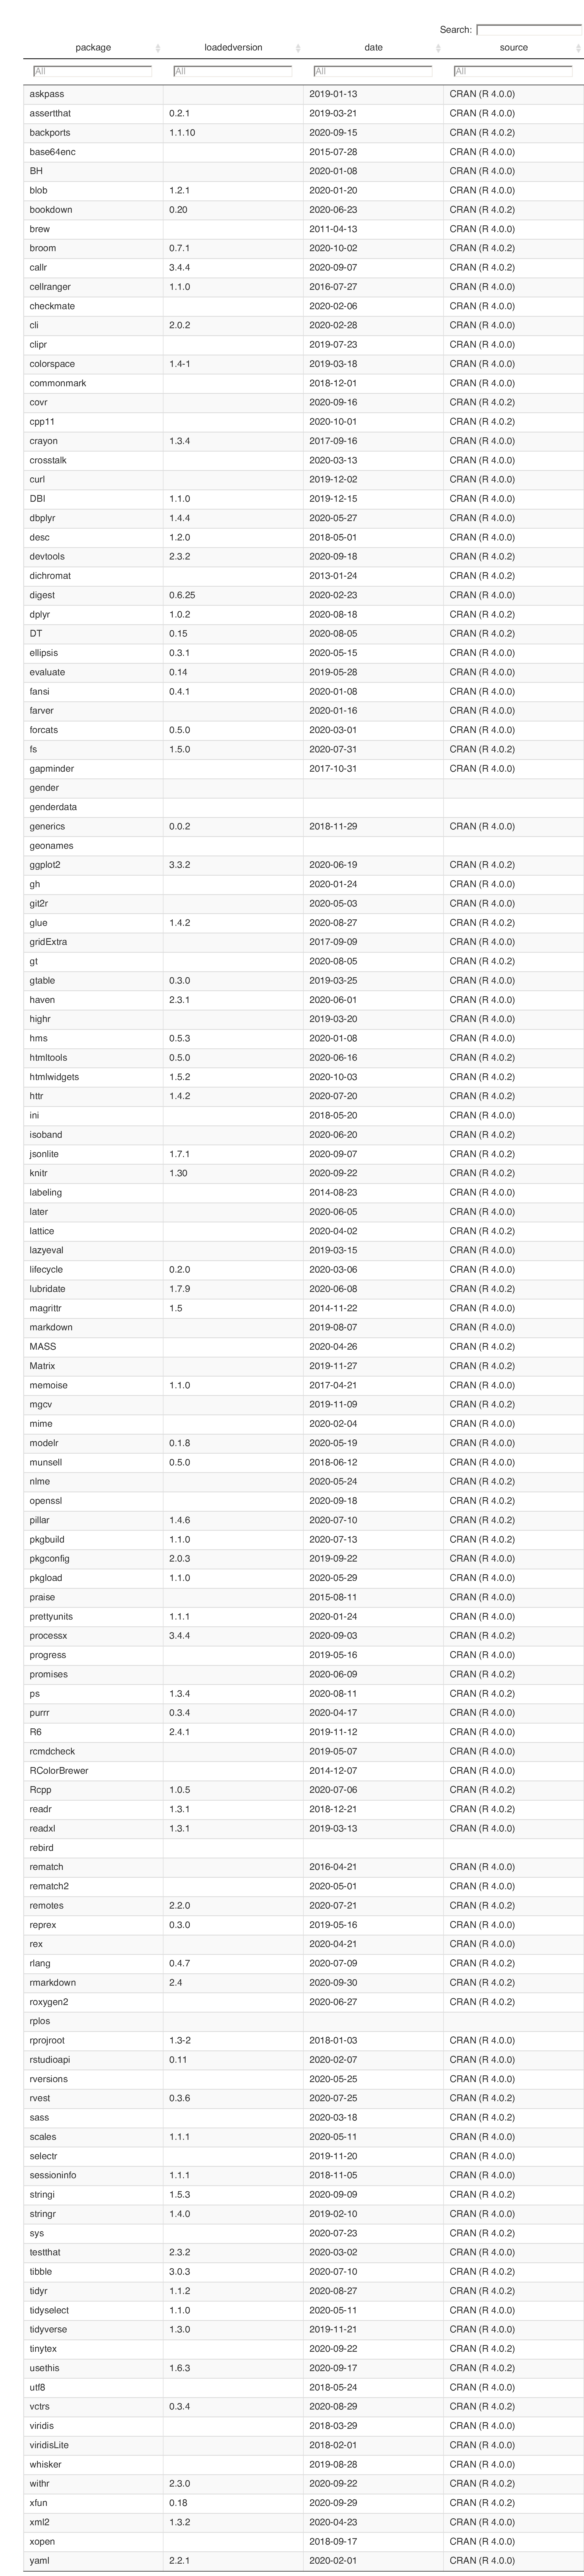
\includegraphics{index_files/figure-latex/unnamed-chunk-3-1.pdf}

\hypertarget{license}{%
\section*{License}\label{license}}
\addcontentsline{toc}{section}{License}

This work is licensed under a \href{https://creativecommons.org/licenses/by-sa/4.0/}{Creative Commons Attribution-ShareAlike 4.0 International License}.

\emph{This is a human-readable summary of (and not a substitute for) the license.
Please see \url{https://creativecommons.org/licenses/by-sa/4.0/legalcode} for the full legal text.}

\textbf{You are free to:}

\begin{itemize}
\item
  \textbf{Share}---copy and redistribute the material in any medium or
  format
\item
  \textbf{Remix}---remix, transform, and build upon the material for any
  purpose, even commercially.
\end{itemize}

The licensor cannot revoke these freedoms as long as you follow the
license terms.

\textbf{Under the following terms:}

\begin{itemize}
\item
  \textbf{Attribution}---You must give appropriate credit, provide a link
  to the license, and indicate if changes were made. You may do so in
  any reasonable manner, but not in any way that suggests the licensor
  endorses you or your use.
\item
  \textbf{ShareAlike}---If you remix, transform, or build upon the material, you must distribute your contributions under the same license as the original.
\item
  \textbf{No additional restrictions}---You may not apply legal terms or
  technological measures that legally restrict others from doing
  anything the license permits.
\end{itemize}

\textbf{Notices:}

You do not have to comply with the license for elements of the
material in the public domain or where your use is permitted by an
applicable exception or limitation.

No warranties are given. The license may not give you all of the
permissions necessary for your intended use. For example, other rights
such as publicity, privacy, or moral rights may limit how you use the
material.

\hypertarget{part-get-your-r-act-together}{%
\part{Get your R act together}\label{part-get-your-r-act-together}}

\hypertarget{install}{%
\chapter{Install R and RStudio}\label{install}}

\hypertarget{r-and-rstudio}{%
\section{R and RStudio}\label{r-and-rstudio}}

\begin{itemize}
\item
  Install \href{https://www.r-project.org}{R, a free software environment for statistical computing and graphics} from \href{https://cloud.r-project.org}{CRAN}, the Comprehensive R Archive Network. I \textbf{highly recommend} you install a precompiled binary distribution for your operating system -- use the links up at the top of the CRAN page linked above!
\item
  Install RStudio's IDE (stands for \emph{integrated development environment}), a powerful user interface for R. Get the Open Source Edition of RStudio Desktop.

  \begin{itemize}
  \tightlist
  \item
    I \textbf{highly recommend} you run the \href{https://www.rstudio.com/products/rstudio/download/preview/}{Preview version}. I find these quite stable and you'll get the cool new features! Update to new Preview versions often.
  \item
    Of course, there are also official releases available \href{https://www.rstudio.com/products/rstudio/\#Desktop}{here}.
  \item
    RStudio comes with a \textbf{text editor}, so there is no immediate need to install a separate stand-alone editor.
  \item
    RStudio can \textbf{interface with Git(Hub)}. However, you must do all the Git(Hub) set up described elsewhere (see \href{https://happygitwithr.com}{Happy Git and GitHub for the useR}) before you can take advantage of this.
  \end{itemize}
\end{itemize}

If you have a pre-existing installation of R and/or RStudio, we \textbf{highly recommend} that you reinstall both and get as current as possible. It can be considerably harder to run old software than new.

\begin{itemize}
\item
  If you upgrade R, you will need to update any packages you have installed. The command below should get you started, though you may need to specify more arguments if, e.g., you have been using a non-default library for your packages.

\begin{Shaded}
\begin{Highlighting}[]
\KeywordTok{update.packages}\NormalTok{(}\DataTypeTok{ask =} \OtherTok{FALSE}\NormalTok{, }\DataTypeTok{checkBuilt =} \OtherTok{TRUE}\NormalTok{)}
\end{Highlighting}
\end{Shaded}

  \textbf{Note:} this will only look for updates on CRAN. So if you use a package that lives \emph{only} on GitHub or if you want a development version from GitHub, you will need to update manually, e.g.~via \texttt{devtools::install\_github()}.
\end{itemize}

\hypertarget{testing-testing}{%
\section{Testing testing}\label{testing-testing}}

\begin{itemize}
\item
  Do whatever is appropriate for your OS to launch RStudio. You should get a window similar to the screenshot you see \href{https://www.rstudio.com/wp-content/uploads/2014/04/rstudio-workbench.png}{here}, but yours will be more boring because you haven't written any code or made any figures yet!
\item
  Put your cursor in the pane labelled Console, which is where you interact with the live R process. Create a simple object with code like \texttt{x\ \textless{}-\ 2\ *\ 4} (followed by enter or return). Then inspect the \texttt{x} object by typing \texttt{x} followed by enter or return. You should see the value 8 print to screen. If yes, you've succeeded in installing R and RStudio.
\end{itemize}

\hypertarget{add-on-packages}{%
\section{Add-on packages}\label{add-on-packages}}

R is an extensible system and many people share useful code they have developed as a \emph{package} via CRAN and GitHub. To install a package from CRAN, for example the \href{https://dplyr.tidyverse.org}{dplyr} package for data manipulation, here is one way to do it in the R console (there are others).

\begin{Shaded}
\begin{Highlighting}[]
\KeywordTok{install.packages}\NormalTok{(}\StringTok{"dplyr"}\NormalTok{, }\DataTypeTok{dependencies =} \OtherTok{TRUE}\NormalTok{)}
\end{Highlighting}
\end{Shaded}

By including \texttt{dependencies\ =\ TRUE}, we are being explicit and extra-careful to install any additional packages the target package, dplyr in the example above, needs to have around.

You could use the above method to install the following packages, all of which we will use:

\begin{itemize}
\tightlist
\item
  \href{https://tidyr.tidyverse.org}{tidyr}
\item
  \href{https://ggplot2.tidyverse.org}{ggplot2}
\end{itemize}

\hypertarget{further-resources}{%
\section{Further resources}\label{further-resources}}

The above will get your basic setup ready but here are some links if you are interested in reading a bit further.

\begin{itemize}
\tightlist
\item
  \href{https://support.rstudio.com/hc/en-us}{How to Use RStudio}
\item
  \href{https://support.rstudio.com/hc/en-us/articles/200552336-Getting-Help-with-R}{RStudio's leads for learning R}
\item
  \href{https://cloud.r-project.org/faqs.html}{R FAQ}
\item
  \href{http://cloud.r-project.org/doc/manuals/R-admin.html}{R Installation and Administration}
\item
  \href{https://cloud.r-project.org/doc/manuals/R-admin.html\#Add_002don-packages}{More about add-on packages in the R Installation and Administration Manual}
\end{itemize}

\hypertarget{r-basics}{%
\chapter{R basics and workflows}\label{r-basics}}

\hypertarget{basics-of-working-with-r-at-the-command-line-and-rstudio-goodies}{%
\section{Basics of working with R at the command line and RStudio goodies}\label{basics-of-working-with-r-at-the-command-line-and-rstudio-goodies}}

Launch RStudio/R.

Notice the default panes:

\begin{itemize}
\tightlist
\item
  Console (entire left)
\item
  Environment / History (tabbed in upper right)
\item
  Files / Plots / Packages / Help (tabbed in lower right)
\end{itemize}

\textbf{FYI:} you can change the default location of the panes, among many other things: \href{https://support.rstudio.com/hc/en-us/articles/200549016-Customizing-RStudio}{Customizing RStudio}.

Go into the Console, where we interact with the live R process.

Make an assignment and then inspect the object you just created:

\begin{Shaded}
\begin{Highlighting}[]
\NormalTok{x <-}\StringTok{ }\DecValTok{3} \OperatorTok{*}\StringTok{ }\DecValTok{4}
\NormalTok{x}
\CommentTok{#> [1] 12}
\end{Highlighting}
\end{Shaded}

All R statements where you create objects -- ``assignments'' -- have this form:

\begin{Shaded}
\begin{Highlighting}[]
\NormalTok{objectName <-}\StringTok{ }\NormalTok{value}
\end{Highlighting}
\end{Shaded}

and in my head I hear, e.g., ``x gets 12''.

You will make lots of assignments and the operator \texttt{\textless{}-} is a pain to type. Don't be lazy and use \texttt{=}, although it would work, because it will just sow confusion later. Instead, utilize RStudio's keyboard shortcut: Alt + - (the minus sign).

Notice that RStudio automagically surrounds \texttt{\textless{}-} with spaces, which demonstrates a useful code formatting practice. Code is miserable to read on a good day. Give your eyes a break and use spaces.

RStudio offers many handy \href{https://support.rstudio.com/hc/en-us/articles/200711853-Keyboard-Shortcuts}{keyboard shortcuts}. Also, Alt+Shift+K brings up a keyboard shortcut reference card.

Object names cannot start with a digit and cannot contain certain other characters such as a comma or a space. You will be wise to adopt a \href{https://en.wikipedia.org/wiki/Snake_case}{convention for demarcating words} in names.

\begin{verbatim}
i_use_snake_case
other.people.use.periods
evenOthersUseCamelCase
\end{verbatim}

Make another assignment:

\begin{Shaded}
\begin{Highlighting}[]
\NormalTok{this_is_a_really_long_name <-}\StringTok{ }\FloatTok{2.5}
\end{Highlighting}
\end{Shaded}

To inspect this, try out RStudio's completion facility: type the first few characters, press TAB, add characters until you disambiguate, then press return.

Make another assignment:

\begin{Shaded}
\begin{Highlighting}[]
\NormalTok{jenny_rocks <-}\StringTok{ }\DecValTok{2} \OperatorTok{^}\StringTok{ }\DecValTok{3}
\end{Highlighting}
\end{Shaded}

Let's try to inspect:

\begin{Shaded}
\begin{Highlighting}[]
\NormalTok{jennyrocks}
\CommentTok{#> Error in eval(expr, envir, enclos): object 'jennyrocks' not found}
\NormalTok{jeny_rocks}
\CommentTok{#> Error in eval(expr, envir, enclos): object 'jeny_rocks' not found}
\end{Highlighting}
\end{Shaded}

Implicit contract with the computer / scripting language: Computer will do tedious computation for you. In return, you will be completely precise in your instructions. Typos matter. Case matters. Get better at typing.

R has a mind-blowing collection of built-in functions that are accessed like so:

\begin{Shaded}
\begin{Highlighting}[]
\KeywordTok{functionName}\NormalTok{(}\DataTypeTok{arg1 =}\NormalTok{ val1, }\DataTypeTok{arg2 =}\NormalTok{ val2, and so on)}
\end{Highlighting}
\end{Shaded}

Let's try using \texttt{seq()} which makes regular sequences of numbers and, while we're at it, demo more helpful features of RStudio.

Type \texttt{se} and hit TAB. A pop up shows you possible completions. Specify \texttt{seq()} by typing more to disambiguate or using the up/down arrows to select. Notice the floating tool-tip-type help that pops up, reminding you of a function's arguments. If you want even more help, press F1 as directed to get the full documentation in the help tab of the lower right pane. Now open the parentheses and notice the automatic addition of the closing parenthesis and the placement of cursor in the middle. Type the arguments \texttt{1,\ 10} and hit return. RStudio also exits the parenthetical expression for you. IDEs are great.

\begin{Shaded}
\begin{Highlighting}[]
\KeywordTok{seq}\NormalTok{(}\DecValTok{1}\NormalTok{, }\DecValTok{10}\NormalTok{)}
\CommentTok{#>  [1]  1  2  3  4  5  6  7  8  9 10}
\end{Highlighting}
\end{Shaded}

The above also demonstrates something about how R resolves function arguments. You can always specify in \texttt{name\ =\ value} form. But if you do not, R attempts to resolve by position. So above, it is assumed that we want a sequence \texttt{from\ =\ 1} that goes \texttt{to\ =\ 10}. Since we didn't specify step size, the default value of \texttt{by} in the function definition is used, which ends up being 1 in this case. For functions I call often, I might use this resolve by position for the first
argument or maybe the first two. After that, I always use \texttt{name\ =\ value}.

Make this assignment and notice similar help with quotation marks.

\begin{Shaded}
\begin{Highlighting}[]
\NormalTok{yo <-}\StringTok{ "hello world"}
\end{Highlighting}
\end{Shaded}

If you just make an assignment, you don't get to see the value, so then you're tempted to immediately inspect.

\begin{Shaded}
\begin{Highlighting}[]
\NormalTok{y <-}\StringTok{ }\KeywordTok{seq}\NormalTok{(}\DecValTok{1}\NormalTok{, }\DecValTok{10}\NormalTok{)}
\NormalTok{y}
\CommentTok{#>  [1]  1  2  3  4  5  6  7  8  9 10}
\end{Highlighting}
\end{Shaded}

This common action can be shortened by surrounding the assignment with parentheses, which causes assignment and ``print to screen'' to happen.

\begin{Shaded}
\begin{Highlighting}[]
\NormalTok{(y <-}\StringTok{ }\KeywordTok{seq}\NormalTok{(}\DecValTok{1}\NormalTok{, }\DecValTok{10}\NormalTok{))}
\CommentTok{#>  [1]  1  2  3  4  5  6  7  8  9 10}
\end{Highlighting}
\end{Shaded}

Not all functions have (or require) arguments:

\begin{Shaded}
\begin{Highlighting}[]
\KeywordTok{date}\NormalTok{()}
\CommentTok{#> [1] "Tue Oct 27 17:42:05 2020"}
\end{Highlighting}
\end{Shaded}

Now look at your workspace -- in the upper right pane. The workspace is where user-defined objects accumulate. You can also get a listing of these objects with commands:

\begin{Shaded}
\begin{Highlighting}[]
\KeywordTok{objects}\NormalTok{()}
\CommentTok{#> [1] "check_quietly"              "install_quietly"           }
\CommentTok{#> [3] "jenny_rocks"                "pretty_install"            }
\CommentTok{#> [5] "shhh_check"                 "this_is_a_really_long_name"}
\CommentTok{#> [7] "x"                          "y"                         }
\CommentTok{#> [9] "yo"}
\KeywordTok{ls}\NormalTok{()}
\CommentTok{#> [1] "check_quietly"              "install_quietly"           }
\CommentTok{#> [3] "jenny_rocks"                "pretty_install"            }
\CommentTok{#> [5] "shhh_check"                 "this_is_a_really_long_name"}
\CommentTok{#> [7] "x"                          "y"                         }
\CommentTok{#> [9] "yo"}
\end{Highlighting}
\end{Shaded}

If you want to remove the object named \texttt{y}, you can do this:

\begin{Shaded}
\begin{Highlighting}[]
\KeywordTok{rm}\NormalTok{(y)}
\end{Highlighting}
\end{Shaded}

To remove everything:

\begin{Shaded}
\begin{Highlighting}[]
\KeywordTok{rm}\NormalTok{(}\DataTypeTok{list =} \KeywordTok{ls}\NormalTok{())}
\end{Highlighting}
\end{Shaded}

or click the broom in RStudio's Environment pane.

\hypertarget{workspace-and-working-directory}{%
\section{Workspace and working directory}\label{workspace-and-working-directory}}

One day you will need to quit R, go do something else and return to your analysis later.

One day you will have multiple analyses going that use R and you want to keep them separate.

One day you will need to bring data from the outside world into R and send numerical results and figures from R back out into the world.

To handle these real life situations, you need to make two decisions:

\begin{itemize}
\tightlist
\item
  What about your analysis is ``real'', i.e.~will you save it as your lasting record of what happened?
\item
  Where does your analysis ``live''?
\end{itemize}

\hypertarget{workspace-.rdata}{%
\subsection{\texorpdfstring{Workspace, \texttt{.RData}}{Workspace, .RData}}\label{workspace-.rdata}}

As a beginning R user, it's OK to consider your workspace ``real''. \emph{Very soon}, I urge you to evolve to the next level, where you consider your saved R scripts as ``real''. (In either case, of course the input data is very much real and requires preservation!) With the input data and the R code you used, you can reproduce
\emph{everything}. You can make your analysis fancier. You can get to the bottom of puzzling results and discover and fix bugs in your code. You can reuse the code to conduct similar analyses in new projects. You can remake a figure with different aspect ratio or save is as TIFF instead of PDF. You are ready to take questions. You are ready for the future.

If you regard your workspace as ``real'' (saving and reloading all the time), if you need to redo analysis \ldots{} you're going to either redo a lot of typing (making mistakes all the way) or will have to mine your R history for the commands you used. Rather than \href{https://support.rstudio.com/hc/en-us/articles/200526217-Command-History}{becoming an expert on managing the R history}, a better use of your time and psychic energy is to keep your ``good'' R code in a script for future reuse.

Because it can be useful sometimes, note the commands you've recently run appear in the History pane.

But you don't have to choose right now and the two strategies are not incompatible. Let's demo the save / reload the workspace approach.

Upon quitting R, you have to decide if you want to save your workspace, for potential restoration the next time you launch R. Depending on your set up, R or your IDE, e.g.~RStudio, will probably prompt you to make this decision.

Quit R/RStudio, either from the menu, using a keyboard shortcut, or by typing \texttt{q()} in the Console. You'll get a prompt like this:

\begin{quote}
Save workspace image to \textasciitilde/.Rdata?
\end{quote}

\emph{Note where the workspace image is to be saved} and then click ``Save''.

Using your favorite method, visit the directory where image was saved and verify there is a file named \texttt{.RData}. You will also see a file \texttt{.Rhistory}, holding the commands submitted in your recent session.

Restart RStudio. In the Console you will see a line like this:

\begin{verbatim}
[Workspace loaded from ~/.RData]
\end{verbatim}

indicating that your workspace has been restored. Look in the Workspace pane and you'll see the same objects as before. In the History tab of the same pane, you should also see your command history. You're back in business. This way of starting and stopping analytical work will not serve you well for long but it's a start.

\hypertarget{working-directory}{%
\subsection{Working directory}\label{working-directory}}

Any process running on your computer has a notion of its ``working directory''. In R, this is where R will look, by default, for files you ask it to load. It also where, by default, any files you write to disk will go. Chances are your current working directory is the directory we inspected above, i.e.~the one where RStudio wanted to save the workspace.

You can explicitly check your working directory with:

\begin{Shaded}
\begin{Highlighting}[]
\KeywordTok{getwd}\NormalTok{()}
\end{Highlighting}
\end{Shaded}

It is also displayed at the top of the RStudio console.

As a beginning R user, it's OK let your home directory or any other weird directory on your computer be R's working directory. \emph{Very soon}, I urge you to evolve to the next level, where you organize your analytical projects into directories and, when working on project A, set R's working directory to the associated directory.

\textbf{Although I do not recommend it}, in case you're curious, you can set R's working directory at the command line like so:

\begin{Shaded}
\begin{Highlighting}[]
\KeywordTok{setwd}\NormalTok{(}\StringTok{"~/myCoolProject"}\NormalTok{)}
\end{Highlighting}
\end{Shaded}

\textbf{Although I do not recommend it}, you can also use RStudio's Files pane to navigate to a directory and then set it as working directory from the menu: \emph{Session \textgreater{} Set Working Directory \textgreater{} To Files Pane Location}. (You'll see even more options there). Or within the Files pane, choose ``More'' and ``Set As Working Directory''.

But there's a better way. A way that also puts you on the path to managing your R work like an expert.

\hypertarget{rprojs}{%
\section{RStudio projects}\label{rprojs}}

Keeping all the files associated with a project organized together -- input data, R scripts, analytical results, figures -- is such a wise and common practice that RStudio has built-in support for this via its \href{https://support.rstudio.com/hc/en-us/articles/200526207-Using-Projects}{\emph{projects}}.

Let's make one to use for the rest of this workshop/class. Do this: \emph{File \textgreater{} New Project\ldots{}}. The directory name you choose here will be the project name. Call it whatever you want (or follow me for convenience).

I created a directory and, therefore RStudio project, called \texttt{swc} in my \texttt{tmp} directory, FYI.

\begin{Shaded}
\begin{Highlighting}[]
\KeywordTok{setwd}\NormalTok{(}\StringTok{"~/tmp/swc"}\NormalTok{)}
\end{Highlighting}
\end{Shaded}

Now check that the ``home'' directory for your project is the working directory of our current R process:

\begin{Shaded}
\begin{Highlighting}[]
\KeywordTok{getwd}\NormalTok{()}
\end{Highlighting}
\end{Shaded}

\emph{I can't print my output here because this document itself does not reside in the RStudio Project we just created.}

Let's enter a few commands in the Console, as if we are just beginning a project:

\begin{Shaded}
\begin{Highlighting}[]
\NormalTok{a <-}\StringTok{ }\DecValTok{2}
\NormalTok{b <-}\StringTok{ }\DecValTok{-3}
\NormalTok{sig_sq <-}\StringTok{ }\FloatTok{0.5}
\NormalTok{x <-}\StringTok{ }\KeywordTok{runif}\NormalTok{(}\DecValTok{40}\NormalTok{)}
\NormalTok{y <-}\StringTok{ }\NormalTok{a }\OperatorTok{+}\StringTok{ }\NormalTok{b }\OperatorTok{*}\StringTok{ }\NormalTok{x }\OperatorTok{+}\StringTok{ }\KeywordTok{rnorm}\NormalTok{(}\DecValTok{40}\NormalTok{, }\DataTypeTok{sd =} \KeywordTok{sqrt}\NormalTok{(sig_sq))}
\NormalTok{(avg_x <-}\StringTok{ }\KeywordTok{mean}\NormalTok{(x))}
\CommentTok{#> [1] 0.52}
\KeywordTok{write}\NormalTok{(avg_x, }\StringTok{"avg_x.txt"}\NormalTok{)}
\KeywordTok{plot}\NormalTok{(x, y)}
\KeywordTok{abline}\NormalTok{(a, b, }\DataTypeTok{col =} \StringTok{"purple"}\NormalTok{)}
\end{Highlighting}
\end{Shaded}

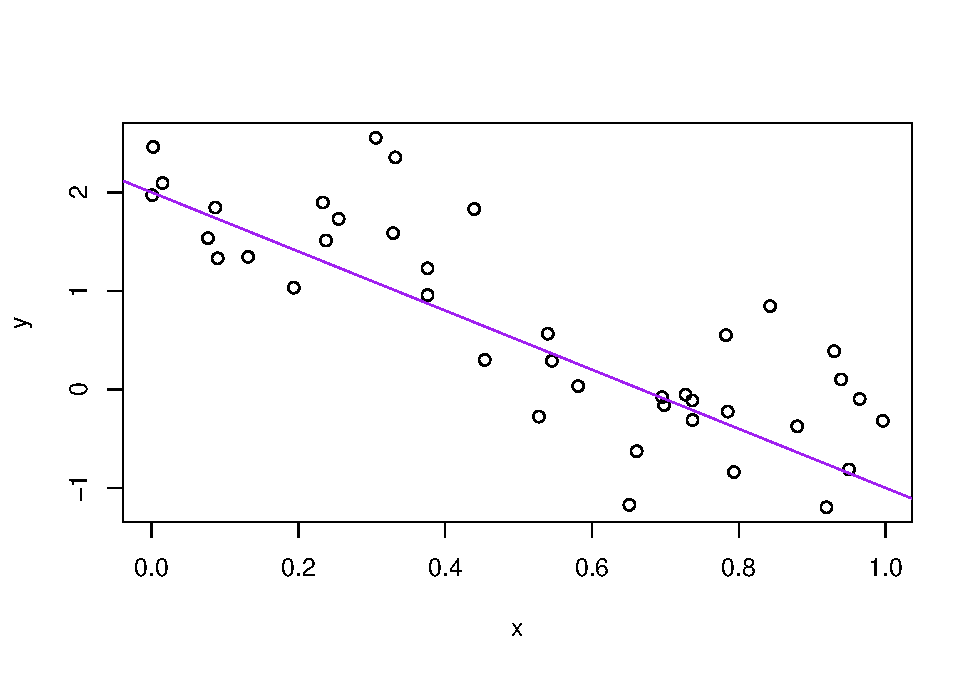
\includegraphics{02_r-basics_files/figure-latex/toy-line-1.pdf}

\begin{Shaded}
\begin{Highlighting}[]
\KeywordTok{dev.print}\NormalTok{(pdf, }\StringTok{"toy_line_plot.pdf"}\NormalTok{)}
\CommentTok{#> pdf }
\CommentTok{#>   2}
\end{Highlighting}
\end{Shaded}

Let's say this is a good start of an analysis and your ready to start preserving the logic and code. Visit the History tab of the upper right pane. Select these commands. Click ``To Source''. Now you have a new pane containing a nascent R script. Click on the floppy disk to save. Give it a name ending in \texttt{.R} or \texttt{.r}, I used \texttt{toy-line.r} and note that, by default, it will go in the directory associated with your project.

Quit RStudio. Inspect the folder associated with your project if you wish. Maybe view the PDF in an external viewer.

Restart RStudio. Notice that things, by default, restore to where we were earlier, e.g.~objects in the workspace, the command history, which files are open for editing, where we are in the file system browser, the working directory for the R process, etc. These are all Good Things.

Change some things about your code. Top priority would be to set a sample size \texttt{n} at the top, e.g.~\texttt{n\ \textless{}-\ 40}, and then replace all the hard-wired 40's with \texttt{n}. Change some other minor-but-detectable stuff, e.g.~alter the sample size \texttt{n}, the slope of the line \texttt{b},the color of the line \ldots{} whatever. Practice the different ways to re-run the code:

\begin{itemize}
\item
  Walk through line by line by keyboard shortcut (Command+Enter) or mouse (click ``Run'' in the upper right corner of editor pane).
\item
  Source the entire document -- equivalent to entering \texttt{source(\textquotesingle{}toy-line.r\textquotesingle{})} in the Console -- by keyboard shortcut (Shift+Command+S) or mouse (click ``Source'' in the upper right corner of editor pane or select from the mini-menu accessible from the associated down triangle).
\item
  Source with echo from the Source mini-menu.
\end{itemize}

Visit your figure in an external viewer to verify that the PDF is changing as you expect.

In your favorite OS-specific way, search your files for \texttt{toy\_line\_plot.pdf} and presumably you will find the PDF itself (no surprise) but \emph{also the script that created it (\texttt{toy-line.r})}. This latter phenomenon is a huge win. One day you will want to remake a figure or just simply understand where it came from. If you rigorously save figures to file \textbf{with R code and not ever ever ever the mouse or the clipboard}, you will sing my praises one day. Trust me.

\hypertarget{stuff}{%
\section{Stuff}\label{stuff}}

It is traditional to save R scripts with a \texttt{.R} or \texttt{.r} suffix. Follow this convention unless you have some extraordinary reason not to.

Comments start with one or more \texttt{\#} symbols. Use them. RStudio helps you (de)comment selected lines with Ctrl+Shift+C (Windows and Linux) or Command+Shift+C (Mac).

Clean out the workspace, i.e.~pretend like you've just revisited this project after a long absence. The broom icon or \texttt{rm(list\ =\ ls())}. Good idea to do this, restart R (available from the Session menu), re-run your analysis to truly check that the code you're saving is complete and correct (or at least rule out obvious problems!).

This workflow will serve you well in the future:

\begin{itemize}
\tightlist
\item
  Create an RStudio project for an analytical project
\item
  Keep inputs there (we'll soon talk about importing)
\item
  Keep scripts there; edit them, run them in bits or as a whole from there
\item
  Keep outputs there (like the PDF written above)
\end{itemize}

Avoid using the mouse for pieces of your analytical workflow, such as loading a dataset or saving a figure. Terribly important for reproducibility and for making it possible to retrospectively determine how a numerical table or PDF was actually produced (searching on local disk on filename, among \texttt{.R} files, will lead to the relevant script).

Many long-time users never save the workspace, never save \texttt{.RData} files (I'm one of them), never save or consult the history. Once/if you get to that point, there are options available in RStudio to disable the loading of \texttt{.RData} and permanently suppress the prompt on exit to save the workspace (go to \emph{Tools \textgreater{} Options \textgreater{} General}).

For the record, when loading data into R and/or writing outputs to file, you can always specify the absolute path and thereby insulate yourself from the current working directory. This is rarely necessary when using RStudio projects properly.

\hypertarget{part-version-control-and-r-markdown}{%
\part{Version control and R Markdown}\label{part-version-control-and-r-markdown}}

\hypertarget{overview}{%
\chapter*{Overview}\label{overview}}
\addcontentsline{toc}{chapter}{Overview}

Although this part now links out to external resources, if you're working through this material on your own, let this be a nudge to pause around here and think about your workflow. I give you permission to spend some time and energy sorting this out! It can be as or more important than learning a new R function or package. The experts don't talk about this much, because they've already got a workflow and it's something they do almost without thinking.

Working through subsequent material in R Markdown documents, possibly using Git and GitHub to track and share your progress, is a great idea and will leave you more prepared for your future data analysis projects. Typing individual lines of R code is but a small part of data analysis and it pays off to think holistically about your workflow.

\hypertarget{version-control}{%
\chapter{Git, GitHub, and RStudio}\label{version-control}}

At this point in STAT 545, all students receive their own STAT 545 GitHub repository that they will use to develop their course work throughout the rest of the course.

This has two purposes:

\begin{itemize}
\tightlist
\item
  It is helpful for course mechanics, e.g.~homework submission and grading,
  peer review.
\item
  Learning to use Git and GitHub, with R and RStudio, is a legitimate
  pedagogical goal.
\end{itemize}

Our instructions around installation, setup, and early Git usage eventually grew so extensive that we created a dedicated website. This content can now be found here:

\url{https://happygitwithr.com}

\hypertarget{r-markdown}{%
\chapter{R Markdown}\label{r-markdown}}

STAT 545 course work is generally submitted in the form of R Markdown documents. Students submit an \texttt{.Rmd} file, which they have executed or rendered to a \texttt{.md} markdown file. R Markdown is a very accessible way to create computational documents that combine prose and tables and figures produced by R code.

An introductory R Markdown workflow, including how it intersects with Git, GitHub, and RStudio, is now maintained within the Happy Git site:

\href{https://happygitwithr.com/rmd-test-drive.html}{Test drive R Markdown}

\hypertarget{part-data-analysis-1}{%
\part{Data analysis 1}\label{part-data-analysis-1}}

\hypertarget{basic-data-care}{%
\chapter{Basic care and feeding of data in R}\label{basic-data-care}}

\hypertarget{buckle-your-seatbelt}{%
\section{Buckle your seatbelt}\label{buckle-your-seatbelt}}

\emph{Ignore if you don't need this bit of support.}

Now is the time to make sure you are working in an appropriate directory on your computer, probably through the use of an \protect\hyperlink{rprojs}{RStudio project}. Enter \texttt{getwd()} in the Console to see current working directory or, in RStudio, this is displayed in the bar at the top of Console.

You should clean out your workspace. In RStudio, click on the ``Clear'' broom icon from the Environment tab or use \emph{Session \textgreater{} Clear Workspace}. You can also enter \texttt{rm(list\ =\ ls())} in the Console to accomplish same.

Now restart R. This will ensure you don't have any packages loaded from previous calls to \texttt{library()}. In RStudio, use \emph{Session \textgreater{} Restart R}. Otherwise, quit R with \texttt{q()} and re-launch it.

Why do we do this? So that the code you write is complete and re-runnable. If you return to a clean slate often, you will root out hidden dependencies where one snippet of code only works because it relies on objects created by code saved elsewhere or, much worse, never saved at all. Similarly, an aggressive clean slate approach will expose any usage of packages that have not been explicitly loaded.

Finally, open a new R script and develop and run your code from there. In RStudio, use \emph{File \textgreater{} New File \textgreater{} R Script}. Save this script with a name ending in \texttt{.r} or \texttt{.R}, containing no spaces or other funny stuff, and that evokes whatever it is we're doing today. Example: \texttt{cm004\_data-care-feeding.r}.

Another great idea is to do this in an R Markdown document. See \protect\hyperlink{r-markdown}{Test drive R Markdown} for a refresher.

\hypertarget{data-frames-are-awesome}{%
\section{Data frames are awesome}\label{data-frames-are-awesome}}

Whenever you have rectangular, spreadsheet-y data, your default data receptacle in R is a data frame. Do not depart from this without good reason. Data frames are awesome because\ldots{}

\begin{itemize}
\tightlist
\item
  Data frames package related variables neatly together,

  \begin{itemize}
  \tightlist
  \item
    keeping them in sync vis-a-vis row order
  \item
    applying any filtering of observations uniformly
  \end{itemize}
\item
  Most functions for inference, modelling, and graphing are happy to be passed a data frame via a \texttt{data\ =} argument. This has been true in base R for a long time.
\item
  The set of packages known as the \href{https://tidyverse.tidyverse.org}{tidyverse} takes this one step further and explicitly prioritizes the processing of data frames. This includes popular packages like \href{https://dplyr.tidyverse.org}{dplyr} and \href{https://ggplot2.tidyverse.org}{ggplot2}. In fact the tidyverse prioritizes a special flavor of data frame, called a ``tibble''.
\end{itemize}

Data frames -- unlike general arrays or, specifically, matrices in R -- can hold variables of different flavors, such as character data (subject ID or name), quantitative data (white blood cell count), and categorical information (treated vs.~untreated). If you use homogeneous structures, like matrices, for data analysis, you are likely to make the terrible mistake of spreading a dataset out over multiple, unlinked objects. Why? Because you can't put character data, such as subject name, into the numeric matrix that holds white blood cell count. This fragmentation is a Bad Idea.

\hypertarget{get-the-gapminder-data}{%
\section{Get the Gapminder data}\label{get-the-gapminder-data}}

We will work with some of the data from the \href{https://www.gapminder.org}{Gapminder project}. I've released this as an R package called \href{https://github.com/jennybc/gapminder}{gapminder}, so we can install it from CRAN like so:

\begin{Shaded}
\begin{Highlighting}[]
\KeywordTok{install.packages}\NormalTok{(}\StringTok{"gapminder"}\NormalTok{)}
\end{Highlighting}
\end{Shaded}

Now load the package:

\begin{Shaded}
\begin{Highlighting}[]
\KeywordTok{library}\NormalTok{(gapminder)}
\end{Highlighting}
\end{Shaded}

\hypertarget{meet-the-gapminder-data-frame-or-tibble}{%
\section{\texorpdfstring{Meet the \texttt{gapminder} data frame or ``tibble''}{Meet the gapminder data frame or ``tibble''}}\label{meet-the-gapminder-data-frame-or-tibble}}

By loading the gapminder package, we now have access to a data frame by the same name. Get an overview of this with \texttt{str()}, which displays the structure of an object.

\begin{Shaded}
\begin{Highlighting}[]
\KeywordTok{str}\NormalTok{(gapminder)}
\CommentTok{#> tibble [1,704 × 6] (S3: tbl_df/tbl/data.frame)}
\CommentTok{#>  $ country  : Factor w/ 142 levels "Afghanistan",..: 1 1 1 1 1 1 1 ..}
\CommentTok{#>  $ continent: Factor w/ 5 levels "Africa","Americas",..: 3 3 3 3 3 ..}
\CommentTok{#>  $ year     : int [1:1704] 1952 1957 1962 1967 1972 1977 1982 1987 ..}
\CommentTok{#>  $ lifeExp  : num [1:1704] 28.8 30.3 32 34 36.1 ...}
\CommentTok{#>  $ pop      : int [1:1704] 8425333 9240934 10267083 11537966 130794..}
\CommentTok{#>  $ gdpPercap: num [1:1704] 779 821 853 836 740 ...}
\end{Highlighting}
\end{Shaded}

\texttt{str()} will provide a sensible description of almost anything and, worst case, nothing bad can actually happen. When in doubt, just \texttt{str()} some of the recently created objects to get some ideas about what to do next.

We could print the \texttt{gapminder} object itself to screen. However, if you've used R before, you might be reluctant to do this, because large datasets just fill up your Console and provide very little insight.

This is the first big win for \textbf{tibbles}. The tidyverse offers a special case of R's default data frame: the ``tibble'', which is a nod to the actual class of these objects, \texttt{tbl\_df}.

If you have not already done so, install the tidyverse meta-package now:

\begin{Shaded}
\begin{Highlighting}[]
\KeywordTok{install.packages}\NormalTok{(}\StringTok{"tidyverse"}\NormalTok{)}
\end{Highlighting}
\end{Shaded}

Now load it:

\begin{Shaded}
\begin{Highlighting}[]
\KeywordTok{library}\NormalTok{(tidyverse)}
\CommentTok{#> ── Attaching packages ──────────────────────────── tidyverse 1.3.0 ──}
\CommentTok{#> ✓ ggplot2 3.3.2     ✓ purrr   0.3.4}
\CommentTok{#> ✓ tibble  3.0.3     ✓ dplyr   1.0.2}
\CommentTok{#> ✓ tidyr   1.1.2     ✓ stringr 1.4.0}
\CommentTok{#> ✓ readr   1.3.1     ✓ forcats 0.5.0}
\CommentTok{#> ── Conflicts ─────────────────────────────── tidyverse_conflicts() ──}
\CommentTok{#> x dplyr::filter() masks stats::filter()}
\CommentTok{#> x dplyr::lag()    masks stats::lag()}
\end{Highlighting}
\end{Shaded}

Now we can boldly print \texttt{gapminder} to screen! It is a tibble (and also a regular data frame) and the tidyverse provides a nice print method that shows the most important stuff and doesn't fill up your Console.

\begin{Shaded}
\begin{Highlighting}[]
\CommentTok{## see? it's still a regular data frame, but also a tibble}
\KeywordTok{class}\NormalTok{(gapminder)}
\CommentTok{#> [1] "tbl_df"     "tbl"        "data.frame"}
\NormalTok{gapminder}
\CommentTok{#> # A tibble: 1,704 x 6}
\CommentTok{#>    country     continent  year lifeExp      pop gdpPercap}
\CommentTok{#>    <fct>       <fct>     <int>   <dbl>    <int>     <dbl>}
\CommentTok{#>  1 Afghanistan Asia       1952    28.8  8425333      779.}
\CommentTok{#>  2 Afghanistan Asia       1957    30.3  9240934      821.}
\CommentTok{#>  3 Afghanistan Asia       1962    32.0 10267083      853.}
\CommentTok{#>  4 Afghanistan Asia       1967    34.0 11537966      836.}
\CommentTok{#>  5 Afghanistan Asia       1972    36.1 13079460      740.}
\CommentTok{#>  6 Afghanistan Asia       1977    38.4 14880372      786.}
\CommentTok{#>  7 Afghanistan Asia       1982    39.9 12881816      978.}
\CommentTok{#>  8 Afghanistan Asia       1987    40.8 13867957      852.}
\CommentTok{#>  9 Afghanistan Asia       1992    41.7 16317921      649.}
\CommentTok{#> 10 Afghanistan Asia       1997    41.8 22227415      635.}
\CommentTok{#> # … with 1,694 more rows}
\end{Highlighting}
\end{Shaded}

If you are dealing with plain vanilla data frames, you can rein in data frame printing explicitly with \texttt{head()} and \texttt{tail()}. Or turn it into a tibble with \texttt{as\_tibble()}!

\begin{Shaded}
\begin{Highlighting}[]
\KeywordTok{head}\NormalTok{(gapminder)}
\CommentTok{#> # A tibble: 6 x 6}
\CommentTok{#>   country     continent  year lifeExp      pop gdpPercap}
\CommentTok{#>   <fct>       <fct>     <int>   <dbl>    <int>     <dbl>}
\CommentTok{#> 1 Afghanistan Asia       1952    28.8  8425333      779.}
\CommentTok{#> 2 Afghanistan Asia       1957    30.3  9240934      821.}
\CommentTok{#> 3 Afghanistan Asia       1962    32.0 10267083      853.}
\CommentTok{#> 4 Afghanistan Asia       1967    34.0 11537966      836.}
\CommentTok{#> 5 Afghanistan Asia       1972    36.1 13079460      740.}
\CommentTok{#> 6 Afghanistan Asia       1977    38.4 14880372      786.}
\KeywordTok{tail}\NormalTok{(gapminder)}
\CommentTok{#> # A tibble: 6 x 6}
\CommentTok{#>   country  continent  year lifeExp      pop gdpPercap}
\CommentTok{#>   <fct>    <fct>     <int>   <dbl>    <int>     <dbl>}
\CommentTok{#> 1 Zimbabwe Africa     1982    60.4  7636524      789.}
\CommentTok{#> 2 Zimbabwe Africa     1987    62.4  9216418      706.}
\CommentTok{#> 3 Zimbabwe Africa     1992    60.4 10704340      693.}
\CommentTok{#> 4 Zimbabwe Africa     1997    46.8 11404948      792.}
\CommentTok{#> 5 Zimbabwe Africa     2002    40.0 11926563      672.}
\CommentTok{#> 6 Zimbabwe Africa     2007    43.5 12311143      470.}
\KeywordTok{as_tibble}\NormalTok{(iris)}
\CommentTok{#> # A tibble: 150 x 5}
\CommentTok{#>    Sepal.Length Sepal.Width Petal.Length Petal.Width Species}
\CommentTok{#>           <dbl>       <dbl>        <dbl>       <dbl> <fct>  }
\CommentTok{#>  1          5.1         3.5          1.4         0.2 setosa }
\CommentTok{#>  2          4.9         3            1.4         0.2 setosa }
\CommentTok{#>  3          4.7         3.2          1.3         0.2 setosa }
\CommentTok{#>  4          4.6         3.1          1.5         0.2 setosa }
\CommentTok{#>  5          5           3.6          1.4         0.2 setosa }
\CommentTok{#>  6          5.4         3.9          1.7         0.4 setosa }
\CommentTok{#>  7          4.6         3.4          1.4         0.3 setosa }
\CommentTok{#>  8          5           3.4          1.5         0.2 setosa }
\CommentTok{#>  9          4.4         2.9          1.4         0.2 setosa }
\CommentTok{#> 10          4.9         3.1          1.5         0.1 setosa }
\CommentTok{#> # … with 140 more rows}
\end{Highlighting}
\end{Shaded}

More ways to query basic info on a data frame:

\begin{Shaded}
\begin{Highlighting}[]
\KeywordTok{names}\NormalTok{(gapminder)}
\CommentTok{#> [1] "country"   "continent" "year"      "lifeExp"   "pop"      }
\CommentTok{#> [6] "gdpPercap"}
\KeywordTok{ncol}\NormalTok{(gapminder)}
\CommentTok{#> [1] 6}
\KeywordTok{length}\NormalTok{(gapminder)}
\CommentTok{#> [1] 6}
\KeywordTok{dim}\NormalTok{(gapminder)}
\CommentTok{#> [1] 1704    6}
\KeywordTok{nrow}\NormalTok{(gapminder)}
\CommentTok{#> [1] 1704}
\end{Highlighting}
\end{Shaded}

A statistical overview can be obtained with \texttt{summary()}:

\begin{Shaded}
\begin{Highlighting}[]
\KeywordTok{summary}\NormalTok{(gapminder)}
\CommentTok{#>         country        continent        year         lifeExp    }
\CommentTok{#>  Afghanistan:  12   Africa  :624   Min.   :1952   Min.   :23.6  }
\CommentTok{#>  Albania    :  12   Americas:300   1st Qu.:1966   1st Qu.:48.2  }
\CommentTok{#>  Algeria    :  12   Asia    :396   Median :1980   Median :60.7  }
\CommentTok{#>  Angola     :  12   Europe  :360   Mean   :1980   Mean   :59.5  }
\CommentTok{#>  Argentina  :  12   Oceania : 24   3rd Qu.:1993   3rd Qu.:70.8  }
\CommentTok{#>  Australia  :  12                  Max.   :2007   Max.   :82.6  }
\CommentTok{#>  (Other)    :1632                                               }
\CommentTok{#>       pop             gdpPercap     }
\CommentTok{#>  Min.   :6.00e+04   Min.   :   241  }
\CommentTok{#>  1st Qu.:2.79e+06   1st Qu.:  1202  }
\CommentTok{#>  Median :7.02e+06   Median :  3532  }
\CommentTok{#>  Mean   :2.96e+07   Mean   :  7215  }
\CommentTok{#>  3rd Qu.:1.96e+07   3rd Qu.:  9325  }
\CommentTok{#>  Max.   :1.32e+09   Max.   :113523  }
\CommentTok{#> }
\end{Highlighting}
\end{Shaded}

Although we haven't begun our formal coverage of visualization yet, it's so important for smell-testing dataset that we will make a few figures anyway. Here we use only base R graphics, which are very basic.

\begin{Shaded}
\begin{Highlighting}[]
\KeywordTok{plot}\NormalTok{(lifeExp }\OperatorTok{~}\StringTok{ }\NormalTok{year, gapminder)}
\end{Highlighting}
\end{Shaded}

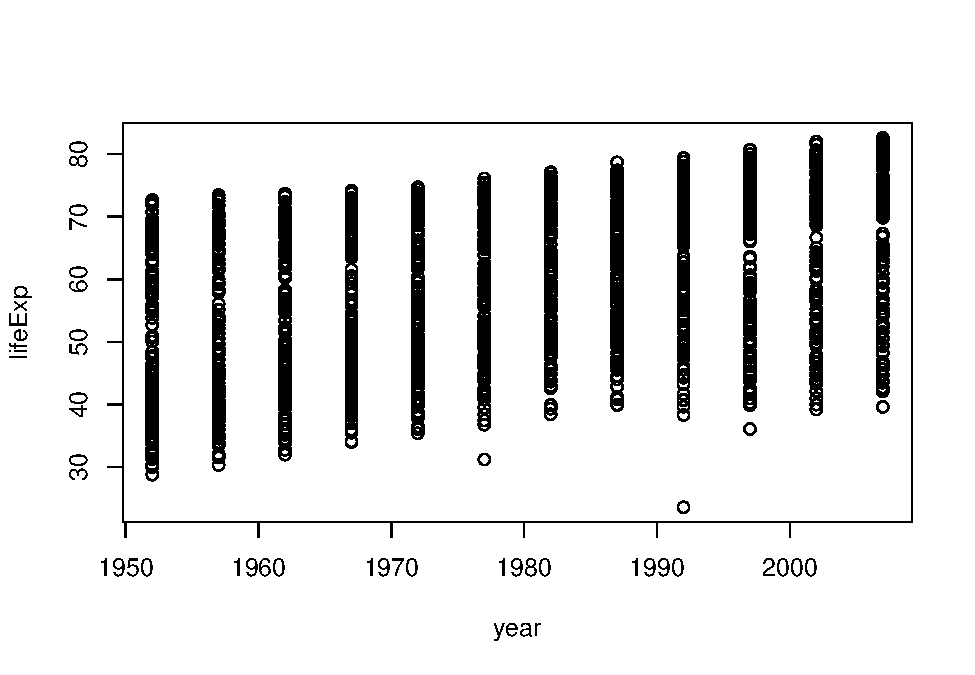
\includegraphics{05_data-care-feeding_files/figure-latex/first-plots-base-R-1.pdf}

\begin{Shaded}
\begin{Highlighting}[]
\KeywordTok{plot}\NormalTok{(lifeExp }\OperatorTok{~}\StringTok{ }\NormalTok{gdpPercap, gapminder)}
\end{Highlighting}
\end{Shaded}

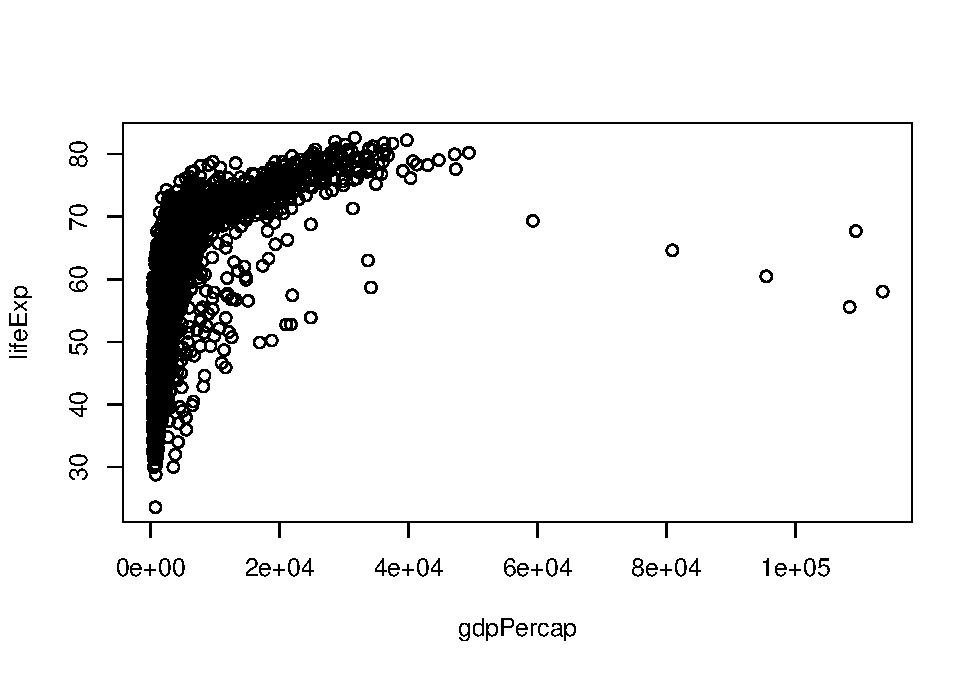
\includegraphics{05_data-care-feeding_files/figure-latex/first-plots-base-R-2.pdf}

\begin{Shaded}
\begin{Highlighting}[]
\KeywordTok{plot}\NormalTok{(lifeExp }\OperatorTok{~}\StringTok{ }\KeywordTok{log}\NormalTok{(gdpPercap), gapminder)}
\end{Highlighting}
\end{Shaded}

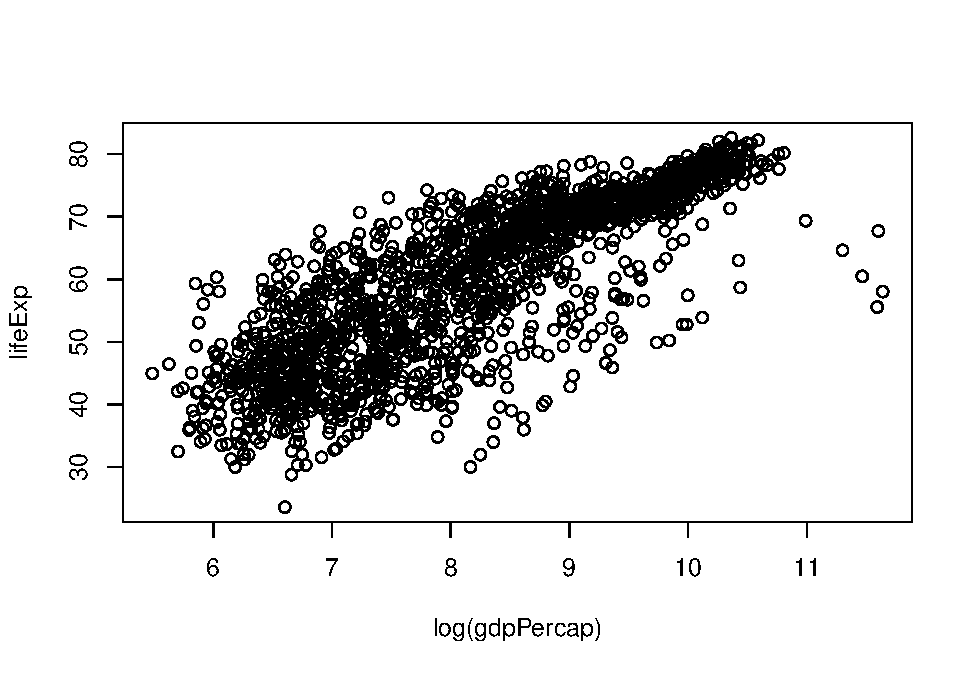
\includegraphics{05_data-care-feeding_files/figure-latex/first-plots-base-R-3.pdf}

Let's go back to the result of \texttt{str()} to talk about what a data frame is.

\begin{Shaded}
\begin{Highlighting}[]
\KeywordTok{str}\NormalTok{(gapminder)}
\CommentTok{#> tibble [1,704 × 6] (S3: tbl_df/tbl/data.frame)}
\CommentTok{#>  $ country  : Factor w/ 142 levels "Afghanistan",..: 1 1 1 1 1 1 1 ..}
\CommentTok{#>  $ continent: Factor w/ 5 levels "Africa","Americas",..: 3 3 3 3 3 ..}
\CommentTok{#>  $ year     : int [1:1704] 1952 1957 1962 1967 1972 1977 1982 1987 ..}
\CommentTok{#>  $ lifeExp  : num [1:1704] 28.8 30.3 32 34 36.1 ...}
\CommentTok{#>  $ pop      : int [1:1704] 8425333 9240934 10267083 11537966 130794..}
\CommentTok{#>  $ gdpPercap: num [1:1704] 779 821 853 836 740 ...}
\end{Highlighting}
\end{Shaded}

A data frame is a special case of a \emph{list}, which is used in R to hold just about anything. Data frames are a special case where the length of each list component is the same. Data frames are superior to matrices in R because they can hold vectors of different flavors, e.g.~numeric, character, and categorical data can be stored together. This comes up a lot!

\hypertarget{look-at-the-variables-inside-a-data-frame}{%
\section{Look at the variables inside a data frame}\label{look-at-the-variables-inside-a-data-frame}}

To specify a single variable from a data frame, use the dollar sign \texttt{\$}. Let's explore the numeric variable for life expectancy.

\begin{Shaded}
\begin{Highlighting}[]
\KeywordTok{head}\NormalTok{(gapminder}\OperatorTok{$}\NormalTok{lifeExp)}
\CommentTok{#> [1] 28.8 30.3 32.0 34.0 36.1 38.4}
\KeywordTok{summary}\NormalTok{(gapminder}\OperatorTok{$}\NormalTok{lifeExp)}
\CommentTok{#>    Min. 1st Qu.  Median    Mean 3rd Qu.    Max. }
\CommentTok{#>    23.6    48.2    60.7    59.5    70.8    82.6}
\KeywordTok{hist}\NormalTok{(gapminder}\OperatorTok{$}\NormalTok{lifeExp)}
\end{Highlighting}
\end{Shaded}

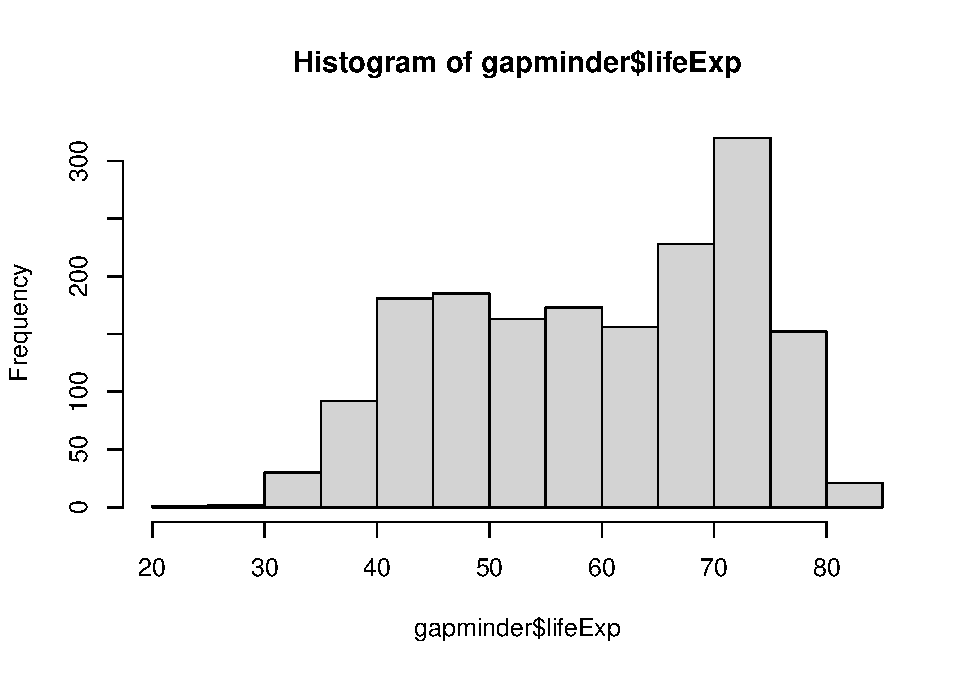
\includegraphics{05_data-care-feeding_files/figure-latex/histogram-lifeExp-1.pdf}

The year variable is an integer variable, but since there are so few unique values it also functions a bit like a categorical variable.

\begin{Shaded}
\begin{Highlighting}[]
\KeywordTok{summary}\NormalTok{(gapminder}\OperatorTok{$}\NormalTok{year)}
\CommentTok{#>    Min. 1st Qu.  Median    Mean 3rd Qu.    Max. }
\CommentTok{#>    1952    1966    1980    1980    1993    2007}
\KeywordTok{table}\NormalTok{(gapminder}\OperatorTok{$}\NormalTok{year)}
\CommentTok{#> }
\CommentTok{#> 1952 1957 1962 1967 1972 1977 1982 1987 1992 1997 2002 2007 }
\CommentTok{#>  142  142  142  142  142  142  142  142  142  142  142  142}
\end{Highlighting}
\end{Shaded}

The variables for country and continent hold truly categorical information, which is stored as a \emph{factor} in R.

\begin{Shaded}
\begin{Highlighting}[]
\KeywordTok{class}\NormalTok{(gapminder}\OperatorTok{$}\NormalTok{continent)}
\CommentTok{#> [1] "factor"}
\KeywordTok{summary}\NormalTok{(gapminder}\OperatorTok{$}\NormalTok{continent)}
\CommentTok{#>   Africa Americas     Asia   Europe  Oceania }
\CommentTok{#>      624      300      396      360       24}
\KeywordTok{levels}\NormalTok{(gapminder}\OperatorTok{$}\NormalTok{continent)}
\CommentTok{#> [1] "Africa"   "Americas" "Asia"     "Europe"   "Oceania"}
\KeywordTok{nlevels}\NormalTok{(gapminder}\OperatorTok{$}\NormalTok{continent)}
\CommentTok{#> [1] 5}
\end{Highlighting}
\end{Shaded}

The \textbf{levels} of the factor \texttt{continent} are ``Africa'', ``Americas'', etc. and this is what's usually presented to your eyeballs by R. In general, the levels are friendly human-readable character strings, like ``male/female'' and ``control/treated''. But \emph{never ever ever} forget that, under the hood, R is really storing integer codes 1, 2, 3, etc. Look at the result from \texttt{str(gapminder\$continent)} if you are skeptical.

\begin{Shaded}
\begin{Highlighting}[]
\KeywordTok{str}\NormalTok{(gapminder}\OperatorTok{$}\NormalTok{continent)}
\CommentTok{#>  Factor w/ 5 levels "Africa","Americas",..: 3 3 3 3 3 3 3 3 3 3 ...}
\end{Highlighting}
\end{Shaded}

This \href{https://en.wikipedia.org/wiki/Janus}{Janus}-like nature of factors means they are rich with booby traps for the unsuspecting but they are a necessary evil. I recommend you resolve to learn how to \protect\hyperlink{factors-boss}{properly care and feed for factors}. The pros far outweigh the cons. Specifically in modelling and figure-making, factors are anticipated and accommodated by the functions and packages you will want to exploit.

Here we count how many observations are associated with each continent and, as usual, try to portray that info visually. This makes it much easier to quickly see that African countries are well represented in this dataset.

\begin{Shaded}
\begin{Highlighting}[]
\KeywordTok{table}\NormalTok{(gapminder}\OperatorTok{$}\NormalTok{continent)}
\CommentTok{#> }
\CommentTok{#>   Africa Americas     Asia   Europe  Oceania }
\CommentTok{#>      624      300      396      360       24}
\KeywordTok{barplot}\NormalTok{(}\KeywordTok{table}\NormalTok{(gapminder}\OperatorTok{$}\NormalTok{continent))}
\end{Highlighting}
\end{Shaded}

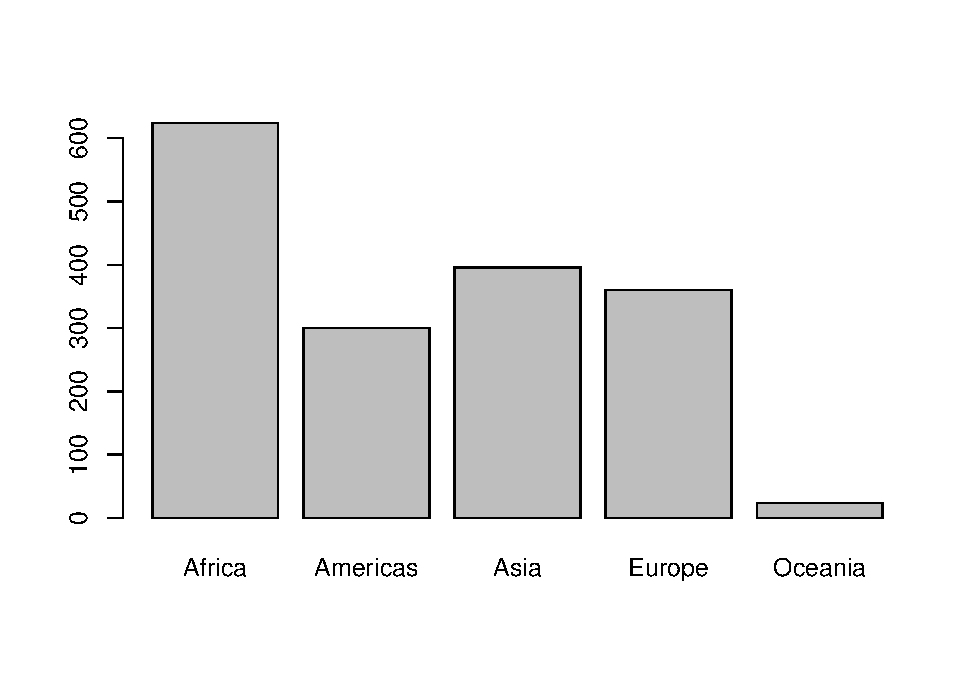
\includegraphics{05_data-care-feeding_files/figure-latex/tabulate-continent-1.pdf}

In the figures below, we see how factors can be put to work in figures. The \texttt{continent} factor is easily mapped into ``facets'' or colors and a legend by the \href{https://ggplot2.tidyverse.org}{ggplot2} package. \emph{Making figures with ggplot2 is covered in Chapter \ref{ggplot2-tutorial} so feel free to just sit back and enjoy these plots or blindly copy/paste.}

\begin{Shaded}
\begin{Highlighting}[]
\CommentTok{## we exploit the fact that ggplot2 was installed and loaded via the tidyverse}
\NormalTok{p <-}\StringTok{ }\KeywordTok{ggplot}\NormalTok{(}\KeywordTok{filter}\NormalTok{(gapminder, continent }\OperatorTok{!=}\StringTok{ "Oceania"}\NormalTok{),}
            \KeywordTok{aes}\NormalTok{(}\DataTypeTok{x =}\NormalTok{ gdpPercap, }\DataTypeTok{y =}\NormalTok{ lifeExp)) }\CommentTok{# just initializes}
\NormalTok{p <-}\StringTok{ }\NormalTok{p }\OperatorTok{+}\StringTok{ }\KeywordTok{scale_x_log10}\NormalTok{() }\CommentTok{# log the x axis the right way}
\NormalTok{p }\OperatorTok{+}\StringTok{ }\KeywordTok{geom_point}\NormalTok{() }\CommentTok{# scatterplot}
\NormalTok{p }\OperatorTok{+}\StringTok{ }\KeywordTok{geom_point}\NormalTok{(}\KeywordTok{aes}\NormalTok{(}\DataTypeTok{color =}\NormalTok{ continent)) }\CommentTok{# map continent to color}
\NormalTok{p }\OperatorTok{+}\StringTok{ }\KeywordTok{geom_point}\NormalTok{(}\DataTypeTok{alpha =}\NormalTok{ (}\DecValTok{1}\OperatorTok{/}\DecValTok{3}\NormalTok{), }\DataTypeTok{size =} \DecValTok{3}\NormalTok{) }\OperatorTok{+}\StringTok{ }\KeywordTok{geom_smooth}\NormalTok{(}\DataTypeTok{lwd =} \DecValTok{3}\NormalTok{, }\DataTypeTok{se =} \OtherTok{FALSE}\NormalTok{)}
\CommentTok{#> `geom_smooth()` using method = 'gam' and formula 'y ~ s(x, bs = "cs")'}
\NormalTok{p }\OperatorTok{+}\StringTok{ }\KeywordTok{geom_point}\NormalTok{(}\DataTypeTok{alpha =}\NormalTok{ (}\DecValTok{1}\OperatorTok{/}\DecValTok{3}\NormalTok{), }\DataTypeTok{size =} \DecValTok{3}\NormalTok{) }\OperatorTok{+}\StringTok{ }\KeywordTok{facet_wrap}\NormalTok{(}\OperatorTok{~}\StringTok{ }\NormalTok{continent) }\OperatorTok{+}
\StringTok{  }\KeywordTok{geom_smooth}\NormalTok{(}\DataTypeTok{lwd =} \FloatTok{1.5}\NormalTok{, }\DataTypeTok{se =} \OtherTok{FALSE}\NormalTok{)}
\CommentTok{#> `geom_smooth()` using method = 'loess' and formula 'y ~ x'}
\end{Highlighting}
\end{Shaded}

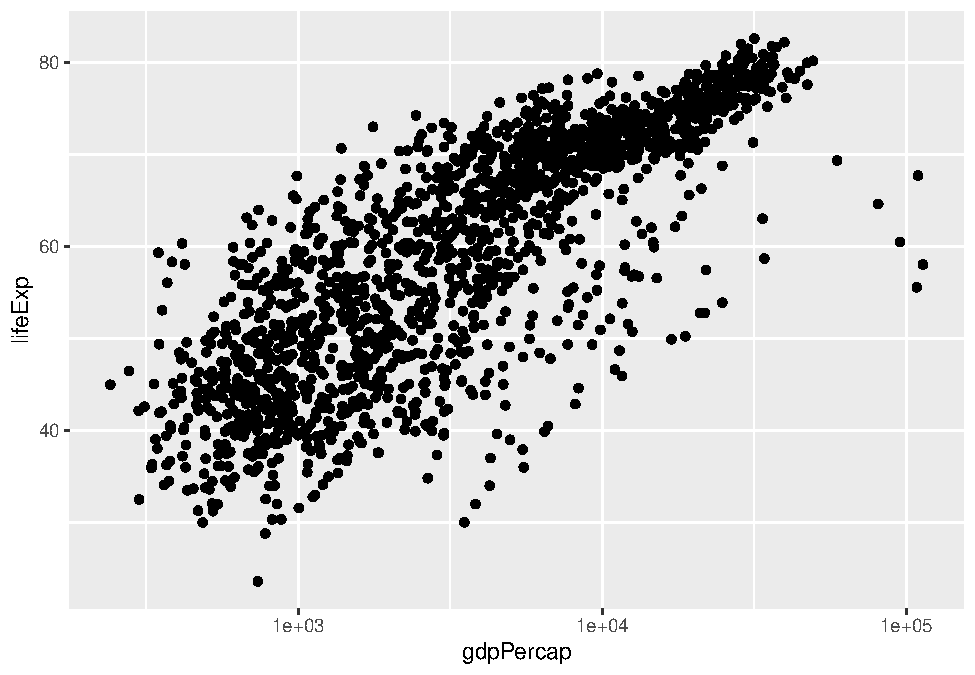
\includegraphics[width=0.49\linewidth]{05_data-care-feeding_files/figure-latex/factors-nice-for-plots-1} 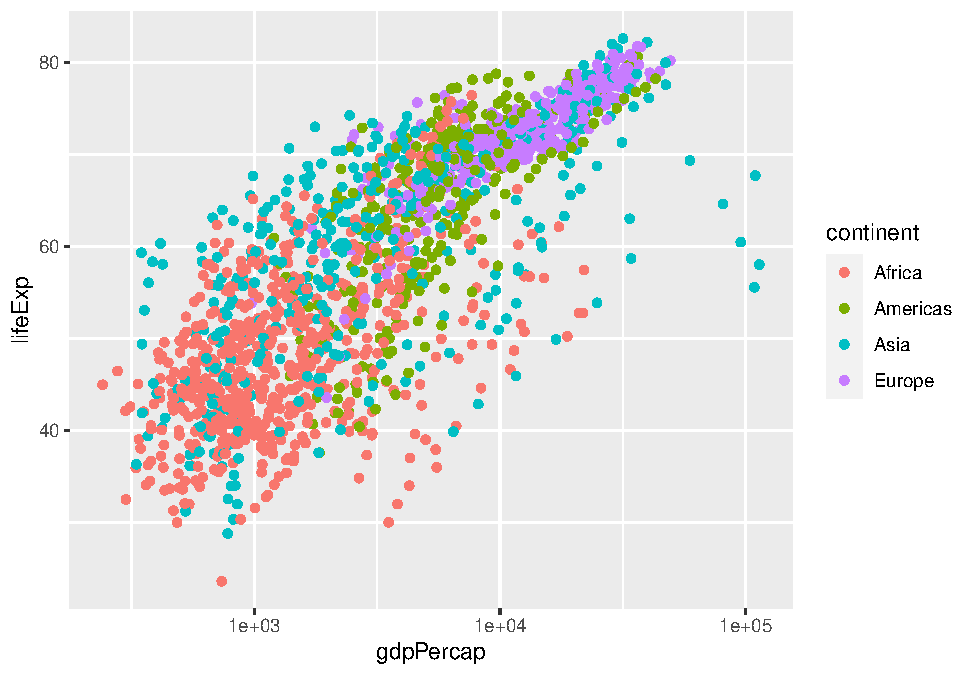
\includegraphics[width=0.49\linewidth]{05_data-care-feeding_files/figure-latex/factors-nice-for-plots-2} 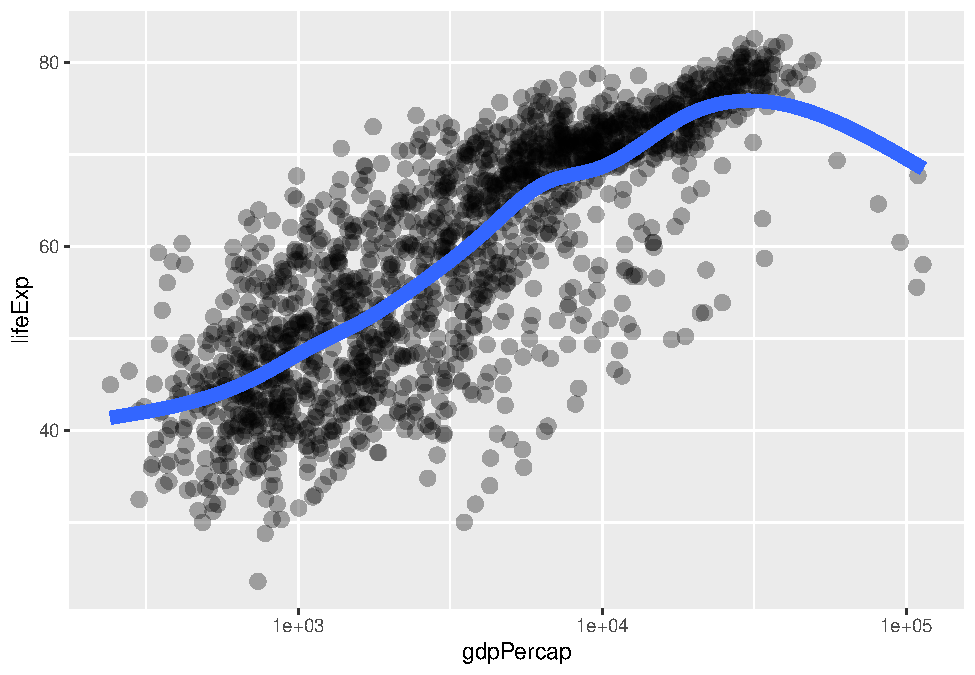
\includegraphics[width=0.49\linewidth]{05_data-care-feeding_files/figure-latex/factors-nice-for-plots-3} 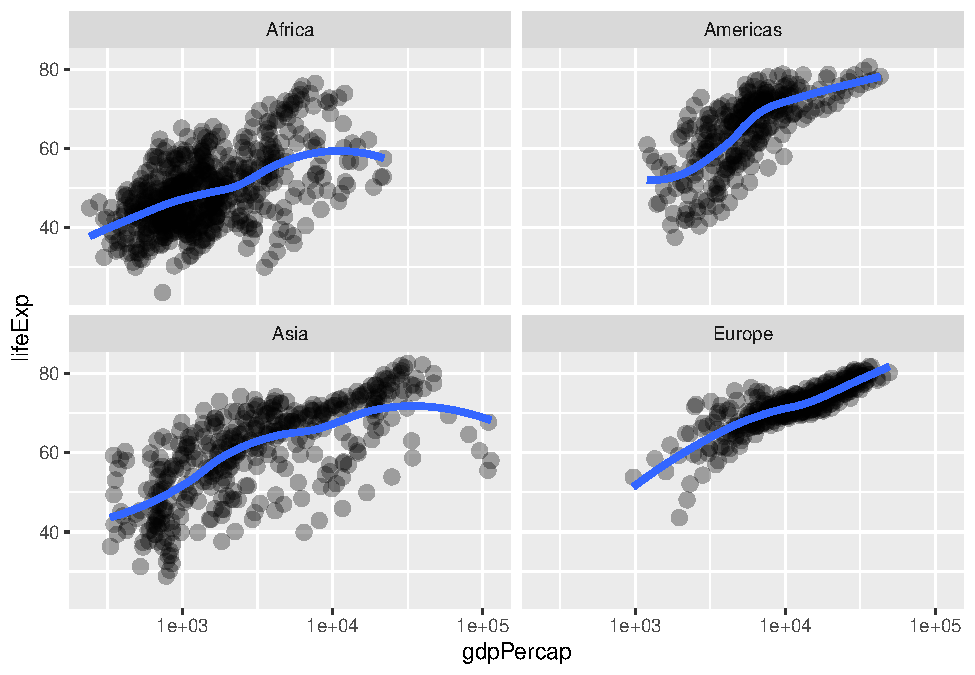
\includegraphics[width=0.49\linewidth]{05_data-care-feeding_files/figure-latex/factors-nice-for-plots-4}

\hypertarget{recap}{%
\section{Recap}\label{recap}}

\begin{itemize}
\item
  Use data frames!!!
\item
  Use the \href{https://tidyverse.tidyverse.org}{tidyverse}!!! This will provide a special type of data frame called a ``tibble'' that has nice default printing behavior, among other benefits.
\item
  When in doubt, \texttt{str()} something or print something.
\item
  Always understand the basic extent of your data frames: number of rows and columns.
\item
  Understand what flavor the variables are.
\item
  Use factors!!! But with intention and care.
\item
  Do basic statistical and visual sanity checking of each variable.
\item
  Refer to variables by name, e.g., \texttt{gapminder\$lifeExp}, not by column number. Your code will be more robust and readable.
\end{itemize}

\hypertarget{dplyr-intro}{%
\chapter{Introduction to dplyr}\label{dplyr-intro}}

\hypertarget{intro}{%
\section{Intro}\label{intro}}

\href{https://dplyr.tidyverse.org}{dplyr} is a package for data manipulation, developed by Hadley Wickham and Romain Francois. It is built to be fast, highly expressive, and open-minded about how your data is stored. It is installed as part of the \href{https://tidyverse.tidyverse.org}{tidyverse} meta-package and, as a core package, it is among those loaded via \texttt{library(tidyverse)}.

dplyr's roots are in an earlier package called \href{http://plyr.had.co.nz}{plyr}, which implements the \href{https://www.jstatsoft.org/article/view/v040i01}{``split-apply-combine'' strategy for data analysis} \citep{wickham2011a}. Where plyr covers a diverse set of inputs and outputs (e.g., arrays, data frames, lists), dplyr has a laser-like focus on data frames or, in the tidyverse, ``tibbles''. dplyr is a package-level treatment of the \texttt{ddply()} function from plyr, because ``data frame in, data frame out'' proved to be so incredibly important.

Have no idea what I'm talking about? Not sure if you care? If you use these base R functions: \texttt{subset()}, \texttt{apply()}, \texttt{{[}sl{]}apply()}, \texttt{tapply()}, \texttt{aggregate()}, \texttt{split()}, \texttt{do.call()}, \texttt{with()}, \texttt{within()}, then you should keep reading. Also, if you use \texttt{for()} loops a lot, you might enjoy learning other ways to iterate over rows or groups of rows or variables in a data frame.

\hypertarget{load-dplyr-and-gapminder}{%
\subsection{Load dplyr and gapminder}\label{load-dplyr-and-gapminder}}

I choose to load the tidyverse, which will load dplyr, among other packages we use incidentally below.

\begin{Shaded}
\begin{Highlighting}[]
\KeywordTok{library}\NormalTok{(tidyverse)}
\CommentTok{#> ── Attaching packages ──────────────────────────── tidyverse 1.3.0 ──}
\CommentTok{#> ✓ ggplot2 3.3.2     ✓ purrr   0.3.4}
\CommentTok{#> ✓ tibble  3.0.3     ✓ dplyr   1.0.2}
\CommentTok{#> ✓ tidyr   1.1.2     ✓ stringr 1.4.0}
\CommentTok{#> ✓ readr   1.3.1     ✓ forcats 0.5.0}
\CommentTok{#> ── Conflicts ─────────────────────────────── tidyverse_conflicts() ──}
\CommentTok{#> x dplyr::filter() masks stats::filter()}
\CommentTok{#> x dplyr::lag()    masks stats::lag()}
\end{Highlighting}
\end{Shaded}

Also load \href{https://github.com/jennybc/gapminder}{gapminder}.

\begin{Shaded}
\begin{Highlighting}[]
\KeywordTok{library}\NormalTok{(gapminder)}
\end{Highlighting}
\end{Shaded}

\hypertarget{say-hello-to-the-gapminder-tibble}{%
\subsection{\texorpdfstring{Say hello to the \texttt{gapminder} tibble}{Say hello to the gapminder tibble}}\label{say-hello-to-the-gapminder-tibble}}

The \texttt{gapminder} data frame is a special kind of data frame: a tibble.

\begin{Shaded}
\begin{Highlighting}[]
\NormalTok{gapminder}
\CommentTok{#> # A tibble: 1,704 x 6}
\CommentTok{#>    country     continent  year lifeExp      pop gdpPercap}
\CommentTok{#>    <fct>       <fct>     <int>   <dbl>    <int>     <dbl>}
\CommentTok{#>  1 Afghanistan Asia       1952    28.8  8425333      779.}
\CommentTok{#>  2 Afghanistan Asia       1957    30.3  9240934      821.}
\CommentTok{#>  3 Afghanistan Asia       1962    32.0 10267083      853.}
\CommentTok{#>  4 Afghanistan Asia       1967    34.0 11537966      836.}
\CommentTok{#>  5 Afghanistan Asia       1972    36.1 13079460      740.}
\CommentTok{#>  6 Afghanistan Asia       1977    38.4 14880372      786.}
\CommentTok{#>  7 Afghanistan Asia       1982    39.9 12881816      978.}
\CommentTok{#>  8 Afghanistan Asia       1987    40.8 13867957      852.}
\CommentTok{#>  9 Afghanistan Asia       1992    41.7 16317921      649.}
\CommentTok{#> 10 Afghanistan Asia       1997    41.8 22227415      635.}
\CommentTok{#> # … with 1,694 more rows}
\end{Highlighting}
\end{Shaded}

It's tibble-ness is why we get nice compact printing. For a reminder of the problems with base data frame printing, go type \texttt{iris} in the R Console or, better yet, print a data frame to screen that has lots of columns.

Note how \texttt{gapminder}'s \texttt{class()} includes \texttt{tbl\_df}; the ``tibble'' terminology is a nod to this.

\begin{Shaded}
\begin{Highlighting}[]
\KeywordTok{class}\NormalTok{(gapminder)}
\CommentTok{#> [1] "tbl_df"     "tbl"        "data.frame"}
\end{Highlighting}
\end{Shaded}

There will be some functions, like \texttt{print()}, that know about tibbles and do something special. There will others that do not, like \texttt{summary()}. In which case the regular data frame treatment will happen, because every tibble is also a regular data frame.

To turn any data frame into a tibble use \texttt{as\_tibble()}:

\begin{Shaded}
\begin{Highlighting}[]
\KeywordTok{as_tibble}\NormalTok{(iris)}
\CommentTok{#> # A tibble: 150 x 5}
\CommentTok{#>    Sepal.Length Sepal.Width Petal.Length Petal.Width Species}
\CommentTok{#>           <dbl>       <dbl>        <dbl>       <dbl> <fct>  }
\CommentTok{#>  1          5.1         3.5          1.4         0.2 setosa }
\CommentTok{#>  2          4.9         3            1.4         0.2 setosa }
\CommentTok{#>  3          4.7         3.2          1.3         0.2 setosa }
\CommentTok{#>  4          4.6         3.1          1.5         0.2 setosa }
\CommentTok{#>  5          5           3.6          1.4         0.2 setosa }
\CommentTok{#>  6          5.4         3.9          1.7         0.4 setosa }
\CommentTok{#>  7          4.6         3.4          1.4         0.3 setosa }
\CommentTok{#>  8          5           3.4          1.5         0.2 setosa }
\CommentTok{#>  9          4.4         2.9          1.4         0.2 setosa }
\CommentTok{#> 10          4.9         3.1          1.5         0.1 setosa }
\CommentTok{#> # … with 140 more rows}
\end{Highlighting}
\end{Shaded}

\hypertarget{think-before-you-create-excerpts-of-your-data}{%
\section{Think before you create excerpts of your data \ldots{}}\label{think-before-you-create-excerpts-of-your-data}}

If you feel the urge to store a little snippet of your data:

\begin{Shaded}
\begin{Highlighting}[]
\NormalTok{(canada <-}\StringTok{ }\NormalTok{gapminder[}\DecValTok{241}\OperatorTok{:}\DecValTok{252}\NormalTok{, ])}
\CommentTok{#> # A tibble: 12 x 6}
\CommentTok{#>    country continent  year lifeExp      pop gdpPercap}
\CommentTok{#>    <fct>   <fct>     <int>   <dbl>    <int>     <dbl>}
\CommentTok{#>  1 Canada  Americas   1952    68.8 14785584    11367.}
\CommentTok{#>  2 Canada  Americas   1957    70.0 17010154    12490.}
\CommentTok{#>  3 Canada  Americas   1962    71.3 18985849    13462.}
\CommentTok{#>  4 Canada  Americas   1967    72.1 20819767    16077.}
\CommentTok{#>  5 Canada  Americas   1972    72.9 22284500    18971.}
\CommentTok{#>  6 Canada  Americas   1977    74.2 23796400    22091.}
\CommentTok{#>  7 Canada  Americas   1982    75.8 25201900    22899.}
\CommentTok{#>  8 Canada  Americas   1987    76.9 26549700    26627.}
\CommentTok{#>  9 Canada  Americas   1992    78.0 28523502    26343.}
\CommentTok{#> 10 Canada  Americas   1997    78.6 30305843    28955.}
\CommentTok{#> 11 Canada  Americas   2002    79.8 31902268    33329.}
\CommentTok{#> 12 Canada  Americas   2007    80.7 33390141    36319.}
\end{Highlighting}
\end{Shaded}

Stop and ask yourself \ldots{}

\begin{quote}
Do I want to create mini datasets for each level of some factor (or unique combination of several factors) \ldots{} in order to compute or graph something?
\end{quote}

If YES, \textbf{use proper data aggregation techniques} or faceting in \href{https://ggplot2.tidyverse.org}{ggplot2} -- \textbf{don't subset the data}. Or, more realistic, only subset the data as a temporary measure while you develop your elegant code for computing on or visualizing these data subsets.

If NO, then maybe you really do need to store a copy of a subset of the data. But seriously consider whether you can achieve your goals by simply using the \texttt{subset\ =} argument of, e.g., the \texttt{lm()} function, to limit computation to your excerpt of choice. Lots of functions offer a \texttt{subset\ =} argument!

Copies and excerpts of your data clutter your workspace, invite mistakes, and sow general confusion. Avoid whenever possible.

Reality can also lie somewhere in between. You will find the workflows presented below can help you accomplish your goals with minimal creation of temporary, intermediate objects.

\hypertarget{use-filter-to-subset-data-row-wise}{%
\section{\texorpdfstring{Use \texttt{filter()} to subset data row-wise}{Use filter() to subset data row-wise}}\label{use-filter-to-subset-data-row-wise}}

\texttt{filter()} takes logical expressions and returns the rows for which all are \texttt{TRUE}.

\begin{Shaded}
\begin{Highlighting}[]
\KeywordTok{filter}\NormalTok{(gapminder, lifeExp }\OperatorTok{<}\StringTok{ }\DecValTok{29}\NormalTok{)}
\CommentTok{#> # A tibble: 2 x 6}
\CommentTok{#>   country     continent  year lifeExp     pop gdpPercap}
\CommentTok{#>   <fct>       <fct>     <int>   <dbl>   <int>     <dbl>}
\CommentTok{#> 1 Afghanistan Asia       1952    28.8 8425333      779.}
\CommentTok{#> 2 Rwanda      Africa     1992    23.6 7290203      737.}
\KeywordTok{filter}\NormalTok{(gapminder, country }\OperatorTok{==}\StringTok{ "Rwanda"}\NormalTok{, year }\OperatorTok{>}\StringTok{ }\DecValTok{1979}\NormalTok{)}
\CommentTok{#> # A tibble: 6 x 6}
\CommentTok{#>   country continent  year lifeExp     pop gdpPercap}
\CommentTok{#>   <fct>   <fct>     <int>   <dbl>   <int>     <dbl>}
\CommentTok{#> 1 Rwanda  Africa     1982    46.2 5507565      882.}
\CommentTok{#> 2 Rwanda  Africa     1987    44.0 6349365      848.}
\CommentTok{#> 3 Rwanda  Africa     1992    23.6 7290203      737.}
\CommentTok{#> 4 Rwanda  Africa     1997    36.1 7212583      590.}
\CommentTok{#> 5 Rwanda  Africa     2002    43.4 7852401      786.}
\CommentTok{#> 6 Rwanda  Africa     2007    46.2 8860588      863.}
\KeywordTok{filter}\NormalTok{(gapminder, country }\OperatorTok\StringTok{ }\KeywordTok{c}\NormalTok{(}\StringTok{"Rwanda"}\NormalTok{, }\StringTok{"Afghanistan"}\NormalTok{))}
\CommentTok{#> # A tibble: 24 x 6}
\CommentTok{#>    country     continent  year lifeExp      pop gdpPercap}
\CommentTok{#>    <fct>       <fct>     <int>   <dbl>    <int>     <dbl>}
\CommentTok{#>  1 Afghanistan Asia       1952    28.8  8425333      779.}
\CommentTok{#>  2 Afghanistan Asia       1957    30.3  9240934      821.}
\CommentTok{#>  3 Afghanistan Asia       1962    32.0 10267083      853.}
\CommentTok{#>  4 Afghanistan Asia       1967    34.0 11537966      836.}
\CommentTok{#>  5 Afghanistan Asia       1972    36.1 13079460      740.}
\CommentTok{#>  6 Afghanistan Asia       1977    38.4 14880372      786.}
\CommentTok{#>  7 Afghanistan Asia       1982    39.9 12881816      978.}
\CommentTok{#>  8 Afghanistan Asia       1987    40.8 13867957      852.}
\CommentTok{#>  9 Afghanistan Asia       1992    41.7 16317921      649.}
\CommentTok{#> 10 Afghanistan Asia       1997    41.8 22227415      635.}
\CommentTok{#> # … with 14 more rows}
\end{Highlighting}
\end{Shaded}

Compare with some base R code to accomplish the same things:

\begin{Shaded}
\begin{Highlighting}[]
\NormalTok{gapminder[gapminder}\OperatorTok{$}\NormalTok{lifeExp }\OperatorTok{<}\StringTok{ }\DecValTok{29}\NormalTok{, ] }\CommentTok{## repeat `gapminder`, [i, j] indexing is distracting}
\KeywordTok{subset}\NormalTok{(gapminder, country }\OperatorTok{==}\StringTok{ "Rwanda"}\NormalTok{) }\CommentTok{## almost same as filter; quite nice actually}
\end{Highlighting}
\end{Shaded}

Under no circumstances should you subset your data the way I did at first:

\begin{Shaded}
\begin{Highlighting}[]
\NormalTok{excerpt <-}\StringTok{ }\NormalTok{gapminder[}\DecValTok{241}\OperatorTok{:}\DecValTok{252}\NormalTok{, ]}
\end{Highlighting}
\end{Shaded}

Why is this a terrible idea?

\begin{itemize}
\tightlist
\item
  It is not self-documenting. What is so special about rows 241 through 252?
\item
  It is fragile. This line of code will produce different results if someone changes the row order of \texttt{gapminder}, e.g.~sorts the data earlier in the script.
\end{itemize}

\begin{Shaded}
\begin{Highlighting}[]
\KeywordTok{filter}\NormalTok{(gapminder, country }\OperatorTok{==}\StringTok{ "Canada"}\NormalTok{)}
\end{Highlighting}
\end{Shaded}

This call explains itself and is fairly robust.

\hypertarget{meet-the-new-pipe-operator}{%
\section{Meet the new pipe operator}\label{meet-the-new-pipe-operator}}

Before we go any further, we should exploit the new pipe operator that the tidyverse imports from the \href{https://magrittr.tidyverse.org}{magrittr} package by Stefan Bache. This is going to change your data analytical life. You no longer need to enact multi-operation commands by nesting them inside each other, like so many \href{https://en.wikipedia.org/wiki/Matryoshka_doll}{Russian nesting dolls}. This new syntax leads to code that is much easier to write and to read.

Here's what it looks like: \texttt{\%\textgreater{}\%}. The RStudio keyboard shortcut: Ctrl+Shift+M (Windows), Cmd+Shift+M (Mac).

Let's demo then I'll explain.

\begin{Shaded}
\begin{Highlighting}[]
\NormalTok{gapminder }\OperatorTok\StringTok{ }\KeywordTok{head}\NormalTok{()}
\CommentTok{#> # A tibble: 6 x 6}
\CommentTok{#>   country     continent  year lifeExp      pop gdpPercap}
\CommentTok{#>   <fct>       <fct>     <int>   <dbl>    <int>     <dbl>}
\CommentTok{#> 1 Afghanistan Asia       1952    28.8  8425333      779.}
\CommentTok{#> 2 Afghanistan Asia       1957    30.3  9240934      821.}
\CommentTok{#> 3 Afghanistan Asia       1962    32.0 10267083      853.}
\CommentTok{#> 4 Afghanistan Asia       1967    34.0 11537966      836.}
\CommentTok{#> 5 Afghanistan Asia       1972    36.1 13079460      740.}
\CommentTok{#> 6 Afghanistan Asia       1977    38.4 14880372      786.}
\end{Highlighting}
\end{Shaded}

This is equivalent to \texttt{head(gapminder)}. The pipe operator takes the thing on the left-hand-side and \textbf{pipes} it into the function call on the right-hand-side -- literally, drops it in as the first argument.

Never fear, you can still specify other arguments to this function! To see the first 3 rows of \texttt{gapminder}, we could say \texttt{head(gapminder,\ 3)} or this:

\begin{Shaded}
\begin{Highlighting}[]
\NormalTok{gapminder }\OperatorTok\StringTok{ }\KeywordTok{head}\NormalTok{(}\DecValTok{3}\NormalTok{)}
\CommentTok{#> # A tibble: 3 x 6}
\CommentTok{#>   country     continent  year lifeExp      pop gdpPercap}
\CommentTok{#>   <fct>       <fct>     <int>   <dbl>    <int>     <dbl>}
\CommentTok{#> 1 Afghanistan Asia       1952    28.8  8425333      779.}
\CommentTok{#> 2 Afghanistan Asia       1957    30.3  9240934      821.}
\CommentTok{#> 3 Afghanistan Asia       1962    32.0 10267083      853.}
\end{Highlighting}
\end{Shaded}

I've advised you to think ``gets'' whenever you see the assignment operator, \texttt{\textless{}-}. Similarly, you should think ``then'' whenever you see the pipe operator, \texttt{\%\textgreater{}\%}.

You are probably not impressed yet, but the magic will soon happen.

\hypertarget{use-select-to-subset-the-data-on-variables-or-columns.}{%
\section{\texorpdfstring{Use \texttt{select()} to subset the data on variables or columns.}{Use select() to subset the data on variables or columns.}}\label{use-select-to-subset-the-data-on-variables-or-columns.}}

Back to dplyr\ldots.

Use \texttt{select()} to subset the data on variables or columns. Here's a conventional call:

\begin{Shaded}
\begin{Highlighting}[]
\KeywordTok{select}\NormalTok{(gapminder, year, lifeExp)}
\CommentTok{#> # A tibble: 1,704 x 2}
\CommentTok{#>     year lifeExp}
\CommentTok{#>    <int>   <dbl>}
\CommentTok{#>  1  1952    28.8}
\CommentTok{#>  2  1957    30.3}
\CommentTok{#>  3  1962    32.0}
\CommentTok{#>  4  1967    34.0}
\CommentTok{#>  5  1972    36.1}
\CommentTok{#>  6  1977    38.4}
\CommentTok{#>  7  1982    39.9}
\CommentTok{#>  8  1987    40.8}
\CommentTok{#>  9  1992    41.7}
\CommentTok{#> 10  1997    41.8}
\CommentTok{#> # … with 1,694 more rows}
\end{Highlighting}
\end{Shaded}

And here's the same operation, but written with the pipe operator and piped through \texttt{head()}:

\begin{Shaded}
\begin{Highlighting}[]
\NormalTok{gapminder }\OperatorTok
\StringTok{  }\KeywordTok{select}\NormalTok{(year, lifeExp) }\OperatorTok
\StringTok{  }\KeywordTok{head}\NormalTok{(}\DecValTok{4}\NormalTok{)}
\CommentTok{#> # A tibble: 4 x 2}
\CommentTok{#>    year lifeExp}
\CommentTok{#>   <int>   <dbl>}
\CommentTok{#> 1  1952    28.8}
\CommentTok{#> 2  1957    30.3}
\CommentTok{#> 3  1962    32.0}
\CommentTok{#> 4  1967    34.0}
\end{Highlighting}
\end{Shaded}

Think: ``Take \texttt{gapminder}, then select the variables \texttt{year} and \texttt{lifeExp}, then show the first 4 rows.''

\hypertarget{revel-in-the-convenience}{%
\section{Revel in the convenience}\label{revel-in-the-convenience}}

Here's the data for Cambodia, but only certain variables:

\begin{Shaded}
\begin{Highlighting}[]
\NormalTok{gapminder }\OperatorTok
\StringTok{  }\KeywordTok{filter}\NormalTok{(country }\OperatorTok{==}\StringTok{ "Cambodia"}\NormalTok{) }\OperatorTok
\StringTok{  }\KeywordTok{select}\NormalTok{(year, lifeExp)}
\CommentTok{#> # A tibble: 12 x 2}
\CommentTok{#>     year lifeExp}
\CommentTok{#>    <int>   <dbl>}
\CommentTok{#>  1  1952    39.4}
\CommentTok{#>  2  1957    41.4}
\CommentTok{#>  3  1962    43.4}
\CommentTok{#>  4  1967    45.4}
\CommentTok{#>  5  1972    40.3}
\CommentTok{#>  6  1977    31.2}
\CommentTok{#>  7  1982    51.0}
\CommentTok{#>  8  1987    53.9}
\CommentTok{#>  9  1992    55.8}
\CommentTok{#> 10  1997    56.5}
\CommentTok{#> 11  2002    56.8}
\CommentTok{#> 12  2007    59.7}
\end{Highlighting}
\end{Shaded}

and what a typical base R call would look like:

\begin{Shaded}
\begin{Highlighting}[]
\NormalTok{gapminder[gapminder}\OperatorTok{$}\NormalTok{country }\OperatorTok{==}\StringTok{ "Cambodia"}\NormalTok{, }\KeywordTok{c}\NormalTok{(}\StringTok{"year"}\NormalTok{, }\StringTok{"lifeExp"}\NormalTok{)]}
\CommentTok{#> # A tibble: 12 x 2}
\CommentTok{#>     year lifeExp}
\CommentTok{#>    <int>   <dbl>}
\CommentTok{#>  1  1952    39.4}
\CommentTok{#>  2  1957    41.4}
\CommentTok{#>  3  1962    43.4}
\CommentTok{#>  4  1967    45.4}
\CommentTok{#>  5  1972    40.3}
\CommentTok{#>  6  1977    31.2}
\CommentTok{#>  7  1982    51.0}
\CommentTok{#>  8  1987    53.9}
\CommentTok{#>  9  1992    55.8}
\CommentTok{#> 10  1997    56.5}
\CommentTok{#> 11  2002    56.8}
\CommentTok{#> 12  2007    59.7}
\end{Highlighting}
\end{Shaded}

\hypertarget{pure-predictable-pipeable}{%
\section{Pure, predictable, pipeable}\label{pure-predictable-pipeable}}

We've barely scratched the surface of dplyr but I want to point out key principles you may start to appreciate. If you're new to R or ``programming with data'', feel free skip this section and \protect\hyperlink{dplyr-single}{move on}.

dplyr's verbs, such as \texttt{filter()} and \texttt{select()}, are what's called \href{https://en.wikipedia.org/wiki/Pure_function}{pure functions}. To quote from the \href{http://adv-r.had.co.nz/Functions.html}{Functions chapter} of Wickham's \href{http://adv-r.had.co.nz}{Advanced R} book \citeyearpar{wickham2015a}:

\begin{quote}
The functions that are the easiest to understand and reason about are pure functions: functions that always map the same input to the same output and have no other impact on the workspace. In other words, pure functions have no side effects: they don't affect the state of the world in any way apart from the value they return.
\end{quote}

In fact, these verbs are a special case of pure functions: they take the same flavor of object as input and output. Namely, a data frame or one of the other data receptacles dplyr supports.

And finally, the data is \textbf{always} the very first argument of the verb functions.

This set of deliberate design choices, together with the new pipe operator, produces a highly effective, low friction \href{http://adv-r.had.co.nz/dsl.html}{domain-specific language} for data analysis.

Go to the next Chapter, \protect\hyperlink{dplyr-single}{dplyr functions for a single dataset}, for more dplyr!

\hypertarget{resources}{%
\section{Resources}\label{resources}}

\href{https://dplyr.tidyverse.org}{dplyr} official stuff:

\begin{itemize}
\tightlist
\item
  Package home \href{https://cloud.r-project.org/package=dplyr}{on CRAN}.

  \begin{itemize}
  \tightlist
  \item
    Note there are several vignettes, with the \href{https://dplyr.tidyverse.org/articles/dplyr.html}{Introduction to dplyr} being the most relevant right now.
  \item
    The \href{https://dplyr.tidyverse.org/articles/window-functions.html}{Window functions} one will also be interesting to you now.
  \end{itemize}
\item
  Development home \href{https://github.com/hadley/dplyr}{on GitHub}.
\item
  \href{https://www.dropbox.com/sh/i8qnluwmuieicxc/AAAgt9tIKoIm7WZKIyK25lh6a}{Tutorial HW delivered} (note this links to a DropBox folder) at useR! 2014 conference.
\end{itemize}

\href{https://github.com/rstudio/cheatsheets/raw/master/data-transformation.pdf}{RStudio Data Transformation Cheat Sheet}, covering dplyr. Remember you can get to these via \emph{Help \textgreater{} Cheatsheets.}

\href{https://r4ds.had.co.nz/transform.html}{Data transformation} chapter of \href{https://r4ds.had.co.nz}{R for Data Science} \citep{wickham2016}.

\href{https://github.com/tjmahr/MadR_Pipelines}{``Let the Data Flow: Pipelines in R with dplyr and magrittr''} - Excellent slides on pipelines and dplyr by TJ Mahr, talk given to the Madison R Users Group.

Blog post \href{https://www.dataschool.io/dplyr-tutorial-for-faster-data-manipulation-in-r/}{``Hands-on dplyr tutorial for faster data manipulation in R''} by Data School, that includes a link to an R Markdown document and links to videos.

Chapter \ref{join-cheatsheet} - cheatsheet I made for dplyr join functions (not relevant yet but soon).

\hypertarget{dplyr-single}{%
\chapter{Single table dplyr functions}\label{dplyr-single}}

\hypertarget{where-were-we}{%
\section{Where were we?}\label{where-were-we}}

In Chapter \ref{dplyr-intro}, Introduction to dplyr, we used two very important verbs and an operator:

\begin{itemize}
\tightlist
\item
  \texttt{filter()} for subsetting data with row logic
\item
  \texttt{select()} for subsetting data variable- or column-wise
\item
  the pipe operator \texttt{\%\textgreater{}\%}, which feeds the LHS as the first argument to the expression on the RHS
\end{itemize}

We also discussed dplyr's role inside the tidyverse and tibbles:

\begin{itemize}
\tightlist
\item
  \href{https://dplyr.tidyverse.org}{dplyr} is a core package in the \href{https://tidyverse.tidyverse.org}{tidyverse} meta-package. Since we often make incidental usage of the others, we will load dplyr and the others via \texttt{library(tidyverse)}.
\item
  The tidyverse embraces a special flavor of data frame, called a tibble. The \texttt{gapminder} dataset is stored as a tibble.
\end{itemize}

\hypertarget{load-dplyr-and-gapminder}{%
\section{Load dplyr and gapminder}\label{load-dplyr-and-gapminder}}

I choose to load the tidyverse, which will load dplyr, among other packages we use incidentally below.

\begin{Shaded}
\begin{Highlighting}[]
\KeywordTok{library}\NormalTok{(tidyverse)}
\CommentTok{#> ── Attaching packages ──────────────────────────── tidyverse 1.3.0 ──}
\CommentTok{#> ✓ ggplot2 3.3.2     ✓ purrr   0.3.4}
\CommentTok{#> ✓ tibble  3.0.3     ✓ dplyr   1.0.2}
\CommentTok{#> ✓ tidyr   1.1.2     ✓ stringr 1.4.0}
\CommentTok{#> ✓ readr   1.3.1     ✓ forcats 0.5.0}
\CommentTok{#> ── Conflicts ─────────────────────────────── tidyverse_conflicts() ──}
\CommentTok{#> x dplyr::filter() masks stats::filter()}
\CommentTok{#> x dplyr::lag()    masks stats::lag()}
\end{Highlighting}
\end{Shaded}

Also load \href{https://github.com/jennybc/gapminder}{gapminder}.

\begin{Shaded}
\begin{Highlighting}[]
\KeywordTok{library}\NormalTok{(gapminder)}
\end{Highlighting}
\end{Shaded}

\hypertarget{create-a-copy-of-gapminder}{%
\section{\texorpdfstring{Create a copy of \texttt{gapminder}}{Create a copy of gapminder}}\label{create-a-copy-of-gapminder}}

We're going to make changes to the \texttt{gapminder} tibble. To eliminate any fear that you're damaging the data that comes with the package, we create an explicit copy of \texttt{gapminder} for our experiments.

\begin{Shaded}
\begin{Highlighting}[]
\NormalTok{(my_gap <-}\StringTok{ }\NormalTok{gapminder)}
\CommentTok{#> # A tibble: 1,704 x 6}
\CommentTok{#>    country     continent  year lifeExp      pop gdpPercap}
\CommentTok{#>    <fct>       <fct>     <int>   <dbl>    <int>     <dbl>}
\CommentTok{#>  1 Afghanistan Asia       1952    28.8  8425333      779.}
\CommentTok{#>  2 Afghanistan Asia       1957    30.3  9240934      821.}
\CommentTok{#>  3 Afghanistan Asia       1962    32.0 10267083      853.}
\CommentTok{#>  4 Afghanistan Asia       1967    34.0 11537966      836.}
\CommentTok{#>  5 Afghanistan Asia       1972    36.1 13079460      740.}
\CommentTok{#>  6 Afghanistan Asia       1977    38.4 14880372      786.}
\CommentTok{#>  7 Afghanistan Asia       1982    39.9 12881816      978.}
\CommentTok{#>  8 Afghanistan Asia       1987    40.8 13867957      852.}
\CommentTok{#>  9 Afghanistan Asia       1992    41.7 16317921      649.}
\CommentTok{#> 10 Afghanistan Asia       1997    41.8 22227415      635.}
\CommentTok{#> # … with 1,694 more rows}
\end{Highlighting}
\end{Shaded}

\textbf{Pay close attention} to when we evaluate statements but let the output just print to screen:

\begin{Shaded}
\begin{Highlighting}[]
\CommentTok{## let output print to screen, but do not store}
\NormalTok{my_gap }\OperatorTok\StringTok{ }\KeywordTok{filter}\NormalTok{(country }\OperatorTok{==}\StringTok{ "Canada"}\NormalTok{)}
\end{Highlighting}
\end{Shaded}

\ldots{} versus when we assign the output to an object, possibly overwriting an existing object.

\begin{Shaded}
\begin{Highlighting}[]
\CommentTok{## store the output as an R object}
\NormalTok{my_precious <-}\StringTok{ }\NormalTok{my_gap }\OperatorTok\StringTok{ }\KeywordTok{filter}\NormalTok{(country }\OperatorTok{==}\StringTok{ "Canada"}\NormalTok{)}
\end{Highlighting}
\end{Shaded}

\hypertarget{use-mutate-to-add-new-variables}{%
\section{\texorpdfstring{Use \texttt{mutate()} to add new variables}{Use mutate() to add new variables}}\label{use-mutate-to-add-new-variables}}

Imagine we wanted to recover each country's GDP. After all, the Gapminder data has a variable for population and GDP per capita. Let's multiply them together.

\texttt{mutate()} is a function that defines and inserts new variables into a tibble. You can refer to existing variables by name.

\begin{Shaded}
\begin{Highlighting}[]
\NormalTok{my_gap }\OperatorTok
\StringTok{  }\KeywordTok{mutate}\NormalTok{(}\DataTypeTok{gdp =}\NormalTok{ pop }\OperatorTok{*}\StringTok{ }\NormalTok{gdpPercap)}
\CommentTok{#> # A tibble: 1,704 x 7}
\CommentTok{#>    country     continent  year lifeExp      pop gdpPercap         gdp}
\CommentTok{#>    <fct>       <fct>     <int>   <dbl>    <int>     <dbl>       <dbl>}
\CommentTok{#>  1 Afghanistan Asia       1952    28.8  8425333      779.     6.57e 9}
\CommentTok{#>  2 Afghanistan Asia       1957    30.3  9240934      821.     7.59e 9}
\CommentTok{#>  3 Afghanistan Asia       1962    32.0 10267083      853.     8.76e 9}
\CommentTok{#>  4 Afghanistan Asia       1967    34.0 11537966      836.     9.65e 9}
\CommentTok{#>  5 Afghanistan Asia       1972    36.1 13079460      740.     9.68e 9}
\CommentTok{#>  6 Afghanistan Asia       1977    38.4 14880372      786.     1.17e10}
\CommentTok{#>  7 Afghanistan Asia       1982    39.9 12881816      978.     1.26e10}
\CommentTok{#>  8 Afghanistan Asia       1987    40.8 13867957      852.     1.18e10}
\CommentTok{#>  9 Afghanistan Asia       1992    41.7 16317921      649.     1.06e10}
\CommentTok{#> 10 Afghanistan Asia       1997    41.8 22227415      635.     1.41e10}
\CommentTok{#> # … with 1,694 more rows}
\end{Highlighting}
\end{Shaded}

Hmmmm \ldots{} those GDP numbers are almost uselessly large and abstract. Consider the \href{https://fivethirtyeight.com/features/xkcd-randall-munroe-qanda-what-if/}{advice of Randall Munroe of xkcd}:

\begin{quote}
One thing that bothers me is large numbers presented without context\ldots{} ``If I added a zero to this number, would the sentence containing it mean something different to me?'' If the answer is ``no'', maybe the number has no business being in the sentence in the first place.
\end{quote}

Maybe it would be more meaningful to consumers of my tables and figures to stick with GDP per capita. But what if I reported GDP per capita, \emph{relative to some benchmark country}. Since Canada is my adopted home, I'll go with that.

I need to create a new variable that is \texttt{gdpPercap} divided by Canadian \texttt{gdpPercap}, taking care that I always divide two numbers that pertain to the same year.

How I achieve this:

\begin{enumerate}
\def\labelenumi{\arabic{enumi}.}
\tightlist
\item
  Filter down to the rows for Canada.
\item
  Create a new temporary variable in \texttt{my\_gap}:

  \begin{enumerate}
  \def\labelenumii{\roman{enumii})}
  \tightlist
  \item
    Extract the \texttt{gdpPercap} variable from the Canadian data.
  \item
    Replicate it once per country in the dataset, so it has the right length.
  \end{enumerate}
\item
  Divide raw \texttt{gdpPercap} by this Canadian figure.
\item
  Discard the temporary variable of replicated Canadian \texttt{gdpPercap}.
\end{enumerate}

\begin{Shaded}
\begin{Highlighting}[]
\NormalTok{ctib <-}\StringTok{ }\NormalTok{my_gap }\OperatorTok
\StringTok{  }\KeywordTok{filter}\NormalTok{(country }\OperatorTok{==}\StringTok{ "Canada"}\NormalTok{)}
\CommentTok{## this is a semi-dangerous way to add this variable}
\CommentTok{## I'd prefer to join on year, but we haven't covered joins yet}
\NormalTok{my_gap <-}\StringTok{ }\NormalTok{my_gap }\OperatorTok
\StringTok{  }\KeywordTok{mutate}\NormalTok{(}\DataTypeTok{tmp =} \KeywordTok{rep}\NormalTok{(ctib}\OperatorTok{$}\NormalTok{gdpPercap, }\KeywordTok{nlevels}\NormalTok{(country)),}
         \DataTypeTok{gdpPercapRel =}\NormalTok{ gdpPercap }\OperatorTok{/}\StringTok{ }\NormalTok{tmp,}
         \DataTypeTok{tmp =} \OtherTok{NULL}\NormalTok{)}
\end{Highlighting}
\end{Shaded}

Note that, \texttt{mutate()} builds new variables sequentially so you can reference earlier ones (like \texttt{tmp}) when defining later ones (like \texttt{gdpPercapRel}). Also, you can get rid of a variable by setting it to \texttt{NULL}.

How could we sanity check that this worked? The Canadian values for \texttt{gdpPercapRel} better all be 1!

\begin{Shaded}
\begin{Highlighting}[]
\NormalTok{my_gap }\OperatorTok\StringTok{ }
\StringTok{  }\KeywordTok{filter}\NormalTok{(country }\OperatorTok{==}\StringTok{ "Canada"}\NormalTok{) }\OperatorTok\StringTok{ }
\StringTok{  }\KeywordTok{select}\NormalTok{(country, year, gdpPercapRel)}
\CommentTok{#> # A tibble: 12 x 3}
\CommentTok{#>    country  year gdpPercapRel}
\CommentTok{#>    <fct>   <int>        <dbl>}
\CommentTok{#>  1 Canada   1952            1}
\CommentTok{#>  2 Canada   1957            1}
\CommentTok{#>  3 Canada   1962            1}
\CommentTok{#>  4 Canada   1967            1}
\CommentTok{#>  5 Canada   1972            1}
\CommentTok{#>  6 Canada   1977            1}
\CommentTok{#>  7 Canada   1982            1}
\CommentTok{#>  8 Canada   1987            1}
\CommentTok{#>  9 Canada   1992            1}
\CommentTok{#> 10 Canada   1997            1}
\CommentTok{#> 11 Canada   2002            1}
\CommentTok{#> 12 Canada   2007            1}
\end{Highlighting}
\end{Shaded}

I perceive Canada to be a ``high GDP'' country, so I predict that the distribution of \texttt{gdpPercapRel} is located below 1, possibly even well below. Check your intuition!

\begin{Shaded}
\begin{Highlighting}[]
\KeywordTok{summary}\NormalTok{(my_gap}\OperatorTok{$}\NormalTok{gdpPercapRel)}
\CommentTok{#>    Min. 1st Qu.  Median    Mean 3rd Qu.    Max. }
\CommentTok{#>    0.01    0.06    0.17    0.33    0.45    9.53}
\end{Highlighting}
\end{Shaded}

The relative GDP per capita numbers are, in general, well below 1. We see that most of the countries covered by this dataset have substantially lower GDP per capita, relative to Canada, across the entire time period.

Remember: Trust No One. Including (especially?) yourself. Always try to find a way to check that you've done what meant to. Prepare to be horrified.

\hypertarget{use-arrange-to-row-order-data-in-a-principled-way}{%
\section{\texorpdfstring{Use \texttt{arrange()} to row-order data in a principled way}{Use arrange() to row-order data in a principled way}}\label{use-arrange-to-row-order-data-in-a-principled-way}}

\texttt{arrange()} reorders the rows in a data frame. Imagine you wanted this data ordered by year then country, as opposed to by country then year.

\begin{Shaded}
\begin{Highlighting}[]
\NormalTok{my_gap }\OperatorTok
\StringTok{  }\KeywordTok{arrange}\NormalTok{(year, country)}
\CommentTok{#> # A tibble: 1,704 x 7}
\CommentTok{#>    country     continent  year lifeExp     pop gdpPercap gdpPercapRel}
\CommentTok{#>    <fct>       <fct>     <int>   <dbl>   <int>     <dbl>        <dbl>}
\CommentTok{#>  1 Afghanistan Asia       1952    28.8  8.43e6      779.       0.0686}
\CommentTok{#>  2 Albania     Europe     1952    55.2  1.28e6     1601.       0.141 }
\CommentTok{#>  3 Algeria     Africa     1952    43.1  9.28e6     2449.       0.215 }
\CommentTok{#>  4 Angola      Africa     1952    30.0  4.23e6     3521.       0.310 }
\CommentTok{#>  5 Argentina   Americas   1952    62.5  1.79e7     5911.       0.520 }
\CommentTok{#>  6 Australia   Oceania    1952    69.1  8.69e6    10040.       0.883 }
\CommentTok{#>  7 Austria     Europe     1952    66.8  6.93e6     6137.       0.540 }
\CommentTok{#>  8 Bahrain     Asia       1952    50.9  1.20e5     9867.       0.868 }
\CommentTok{#>  9 Bangladesh  Asia       1952    37.5  4.69e7      684.       0.0602}
\CommentTok{#> 10 Belgium     Europe     1952    68    8.73e6     8343.       0.734 }
\CommentTok{#> # … with 1,694 more rows}
\end{Highlighting}
\end{Shaded}

Or maybe you want just the data from 2007, sorted on life expectancy?

\begin{Shaded}
\begin{Highlighting}[]
\NormalTok{my_gap }\OperatorTok
\StringTok{  }\KeywordTok{filter}\NormalTok{(year }\OperatorTok{==}\StringTok{ }\DecValTok{2007}\NormalTok{) }\OperatorTok
\StringTok{  }\KeywordTok{arrange}\NormalTok{(lifeExp)}
\CommentTok{#> # A tibble: 142 x 7}
\CommentTok{#>    country      continent  year lifeExp    pop gdpPercap gdpPercapRel}
\CommentTok{#>    <fct>        <fct>     <int>   <dbl>  <int>     <dbl>        <dbl>}
\CommentTok{#>  1 Swaziland    Africa     2007    39.6 1.13e6     4513.       0.124 }
\CommentTok{#>  2 Mozambique   Africa     2007    42.1 2.00e7      824.       0.0227}
\CommentTok{#>  3 Zambia       Africa     2007    42.4 1.17e7     1271.       0.0350}
\CommentTok{#>  4 Sierra Leone Africa     2007    42.6 6.14e6      863.       0.0237}
\CommentTok{#>  5 Lesotho      Africa     2007    42.6 2.01e6     1569.       0.0432}
\CommentTok{#>  6 Angola       Africa     2007    42.7 1.24e7     4797.       0.132 }
\CommentTok{#>  7 Zimbabwe     Africa     2007    43.5 1.23e7      470.       0.0129}
\CommentTok{#>  8 Afghanistan  Asia       2007    43.8 3.19e7      975.       0.0268}
\CommentTok{#>  9 Central Afr… Africa     2007    44.7 4.37e6      706.       0.0194}
\CommentTok{#> 10 Liberia      Africa     2007    45.7 3.19e6      415.       0.0114}
\CommentTok{#> # … with 132 more rows}
\end{Highlighting}
\end{Shaded}

Oh, you'd like to sort on life expectancy in \textbf{desc}ending order? Then use \texttt{desc()}.

\begin{Shaded}
\begin{Highlighting}[]
\NormalTok{my_gap }\OperatorTok
\StringTok{  }\KeywordTok{filter}\NormalTok{(year }\OperatorTok{==}\StringTok{ }\DecValTok{2007}\NormalTok{) }\OperatorTok
\StringTok{  }\KeywordTok{arrange}\NormalTok{(}\KeywordTok{desc}\NormalTok{(lifeExp))}
\CommentTok{#> # A tibble: 142 x 7}
\CommentTok{#>    country     continent  year lifeExp     pop gdpPercap gdpPercapRel}
\CommentTok{#>    <fct>       <fct>     <int>   <dbl>   <int>     <dbl>        <dbl>}
\CommentTok{#>  1 Japan       Asia       2007    82.6  1.27e8    31656.        0.872}
\CommentTok{#>  2 Hong Kong,… Asia       2007    82.2  6.98e6    39725.        1.09 }
\CommentTok{#>  3 Iceland     Europe     2007    81.8  3.02e5    36181.        0.996}
\CommentTok{#>  4 Switzerland Europe     2007    81.7  7.55e6    37506.        1.03 }
\CommentTok{#>  5 Australia   Oceania    2007    81.2  2.04e7    34435.        0.948}
\CommentTok{#>  6 Spain       Europe     2007    80.9  4.04e7    28821.        0.794}
\CommentTok{#>  7 Sweden      Europe     2007    80.9  9.03e6    33860.        0.932}
\CommentTok{#>  8 Israel      Asia       2007    80.7  6.43e6    25523.        0.703}
\CommentTok{#>  9 France      Europe     2007    80.7  6.11e7    30470.        0.839}
\CommentTok{#> 10 Canada      Americas   2007    80.7  3.34e7    36319.        1    }
\CommentTok{#> # … with 132 more rows}
\end{Highlighting}
\end{Shaded}

I advise that your analyses NEVER rely on rows or variables being in a specific order. But it's still true that human beings write the code and the interactive development process can be much nicer if you reorder the rows of your data as you go along. Also, once you are preparing tables for human eyeballs, it is imperative that you step up and take control of row order.

\hypertarget{use-rename-to-rename-variables}{%
\section{\texorpdfstring{Use \texttt{rename()} to rename variables}{Use rename() to rename variables}}\label{use-rename-to-rename-variables}}

When I first cleaned this Gapminder excerpt, I was a \href{https://en.wikipedia.org/wiki/Camel_case}{\texttt{camelCase}} person, but now I'm all about \href{https://en.wikipedia.org/wiki/Snake_case}{\texttt{snake\_case}}. So I am vexed by the variable names I chose when I cleaned this data years ago. Let's rename some variables!

\begin{Shaded}
\begin{Highlighting}[]
\NormalTok{my_gap }\OperatorTok
\StringTok{  }\KeywordTok{rename}\NormalTok{(}\DataTypeTok{life_exp =}\NormalTok{ lifeExp,}
         \DataTypeTok{gdp_percap =}\NormalTok{ gdpPercap,}
         \DataTypeTok{gdp_percap_rel =}\NormalTok{ gdpPercapRel)}
\CommentTok{#> # A tibble: 1,704 x 7}
\CommentTok{#>    country  continent  year life_exp    pop gdp_percap gdp_percap_rel}
\CommentTok{#>    <fct>    <fct>     <int>    <dbl>  <int>      <dbl>          <dbl>}
\CommentTok{#>  1 Afghani… Asia       1952     28.8 8.43e6       779.         0.0686}
\CommentTok{#>  2 Afghani… Asia       1957     30.3 9.24e6       821.         0.0657}
\CommentTok{#>  3 Afghani… Asia       1962     32.0 1.03e7       853.         0.0634}
\CommentTok{#>  4 Afghani… Asia       1967     34.0 1.15e7       836.         0.0520}
\CommentTok{#>  5 Afghani… Asia       1972     36.1 1.31e7       740.         0.0390}
\CommentTok{#>  6 Afghani… Asia       1977     38.4 1.49e7       786.         0.0356}
\CommentTok{#>  7 Afghani… Asia       1982     39.9 1.29e7       978.         0.0427}
\CommentTok{#>  8 Afghani… Asia       1987     40.8 1.39e7       852.         0.0320}
\CommentTok{#>  9 Afghani… Asia       1992     41.7 1.63e7       649.         0.0246}
\CommentTok{#> 10 Afghani… Asia       1997     41.8 2.22e7       635.         0.0219}
\CommentTok{#> # … with 1,694 more rows}
\end{Highlighting}
\end{Shaded}

I did NOT assign the post-rename object back to \texttt{my\_gap} because that would make the chunks in this tutorial harder to copy/paste and run out of order. In real life, I would probably assign this back to \texttt{my\_gap}, in a data preparation script, and proceed with the new variable names.

\hypertarget{select-can-rename-and-reposition-variables}{%
\section{\texorpdfstring{\texttt{select()} can rename and reposition variables}{select() can rename and reposition variables}}\label{select-can-rename-and-reposition-variables}}

You've seen simple use of \texttt{select()}. There are two tricks you might enjoy:

\begin{enumerate}
\def\labelenumi{\arabic{enumi}.}
\tightlist
\item
  \texttt{select()} can rename the variables you request to keep.
\item
  \texttt{select()} can be used with \texttt{everything()} to hoist a variable up to the front of the tibble.
\end{enumerate}

\begin{Shaded}
\begin{Highlighting}[]
\NormalTok{my_gap }\OperatorTok
\StringTok{  }\KeywordTok{filter}\NormalTok{(country }\OperatorTok{==}\StringTok{ "Burundi"}\NormalTok{, year }\OperatorTok{>}\StringTok{ }\DecValTok{1996}\NormalTok{) }\OperatorTok\StringTok{ }
\StringTok{  }\KeywordTok{select}\NormalTok{(}\DataTypeTok{yr =}\NormalTok{ year, lifeExp, gdpPercap) }\OperatorTok\StringTok{ }
\StringTok{  }\KeywordTok{select}\NormalTok{(gdpPercap, }\KeywordTok{everything}\NormalTok{())}
\CommentTok{#> # A tibble: 3 x 3}
\CommentTok{#>   gdpPercap    yr lifeExp}
\CommentTok{#>       <dbl> <int>   <dbl>}
\CommentTok{#> 1      463.  1997    45.3}
\CommentTok{#> 2      446.  2002    47.4}
\CommentTok{#> 3      430.  2007    49.6}
\end{Highlighting}
\end{Shaded}

\texttt{everything()} is one of several helpers for variable selection. Read its help to see the rest.

\hypertarget{group_by-is-a-mighty-weapon}{%
\section{\texorpdfstring{\texttt{group\_by()} is a mighty weapon}{group\_by() is a mighty weapon}}\label{group_by-is-a-mighty-weapon}}

I have found that \sout{friends and family} collaborators love to ask seemingly innocuous questions like, ``which country experienced the sharpest 5-year drop in life expectancy?''. In fact, that is a totally natural question to ask. But if you are using a language that doesn't know about data, it's an incredibly annoying question to answer.

dplyr offers powerful tools to solve this class of problem:

\begin{itemize}
\item
  \texttt{group\_by()} adds extra structure to your dataset -- grouping information -- which lays the groundwork for computations within the groups.
\item
  \texttt{summarize()} takes a dataset with \(n\) observations, computes requested summaries, and returns a dataset with 1 observation.
\item
  Window functions take a dataset with \(n\) observations and return a dataset with \(n\) observations.
\item
  \texttt{mutate()} and \texttt{summarize()} will honor groups.
\item
  You can also do very general computations on your groups with \texttt{do()}, though elsewhere in this course, I advocate for other approaches that I find more intuitive, using the \href{https://purrr.tidyverse.org}{purrr} package.
\end{itemize}

Combined with the verbs you already know, these new tools allow you to solve an extremely diverse set of problems with relative ease.

\hypertarget{counting-things-up}{%
\subsection{Counting things up}\label{counting-things-up}}

Let's start with simple counting. How many observations do we have per continent?

\begin{Shaded}
\begin{Highlighting}[]
\NormalTok{my_gap }\OperatorTok
\StringTok{  }\KeywordTok{group_by}\NormalTok{(continent) }\OperatorTok
\StringTok{  }\KeywordTok{summarize}\NormalTok{(}\DataTypeTok{n =} \KeywordTok{n}\NormalTok{())}
\CommentTok{#> `summarise()` ungrouping output (override with `.groups` argument)}
\CommentTok{#> # A tibble: 5 x 2}
\CommentTok{#>   continent     n}
\CommentTok{#>   <fct>     <int>}
\CommentTok{#> 1 Africa      624}
\CommentTok{#> 2 Americas    300}
\CommentTok{#> 3 Asia        396}
\CommentTok{#> 4 Europe      360}
\CommentTok{#> 5 Oceania      24}
\end{Highlighting}
\end{Shaded}

Let us pause here to think about the tidyverse. You could get these same frequencies using \texttt{table()} from base R.

\begin{Shaded}
\begin{Highlighting}[]
\KeywordTok{table}\NormalTok{(gapminder}\OperatorTok{$}\NormalTok{continent)}
\CommentTok{#> }
\CommentTok{#>   Africa Americas     Asia   Europe  Oceania }
\CommentTok{#>      624      300      396      360       24}
\KeywordTok{str}\NormalTok{(}\KeywordTok{table}\NormalTok{(gapminder}\OperatorTok{$}\NormalTok{continent))}
\CommentTok{#>  'table' int [1:5(1d)] 624 300 396 360 24}
\CommentTok{#>  - attr(*, "dimnames")=List of 1}
\CommentTok{#>   ..$ : chr [1:5] "Africa" "Americas" "Asia" "Europe" ...}
\end{Highlighting}
\end{Shaded}

But the object of class \texttt{table} that is returned makes downstream computation a bit fiddlier than you'd like. For example, it's too bad the continent levels come back only as \emph{names} and not as a proper factor, with the original set of levels. This is an example of how the tidyverse smooths transitions where you want the output of step \texttt{i} to become the input of step \texttt{i\ +\ 1}.

The \texttt{tally()} function is a convenience function that knows to count rows. It honors groups.

\begin{Shaded}
\begin{Highlighting}[]
\NormalTok{my_gap }\OperatorTok
\StringTok{  }\KeywordTok{group_by}\NormalTok{(continent) }\OperatorTok
\StringTok{  }\KeywordTok{tally}\NormalTok{()}
\CommentTok{#> # A tibble: 5 x 2}
\CommentTok{#>   continent     n}
\CommentTok{#>   <fct>     <int>}
\CommentTok{#> 1 Africa      624}
\CommentTok{#> 2 Americas    300}
\CommentTok{#> 3 Asia        396}
\CommentTok{#> 4 Europe      360}
\CommentTok{#> 5 Oceania      24}
\end{Highlighting}
\end{Shaded}

The \texttt{count()} function is an even more convenient function that does both grouping and counting.

\begin{Shaded}
\begin{Highlighting}[]
\NormalTok{my_gap }\OperatorTok\StringTok{ }
\StringTok{  }\KeywordTok{count}\NormalTok{(continent)}
\CommentTok{#> # A tibble: 5 x 2}
\CommentTok{#>   continent     n}
\CommentTok{#>   <fct>     <int>}
\CommentTok{#> 1 Africa      624}
\CommentTok{#> 2 Americas    300}
\CommentTok{#> 3 Asia        396}
\CommentTok{#> 4 Europe      360}
\CommentTok{#> 5 Oceania      24}
\end{Highlighting}
\end{Shaded}

What if we wanted to add the number of unique countries for each continent? You can compute multiple summaries inside \texttt{summarize()}. Use the \texttt{n\_distinct()} function to count the number of distinct countries within each continent.

\begin{Shaded}
\begin{Highlighting}[]
\NormalTok{my_gap }\OperatorTok
\StringTok{  }\KeywordTok{group_by}\NormalTok{(continent) }\OperatorTok
\StringTok{  }\KeywordTok{summarize}\NormalTok{(}\DataTypeTok{n =} \KeywordTok{n}\NormalTok{(),}
            \DataTypeTok{n_countries =} \KeywordTok{n_distinct}\NormalTok{(country))}
\CommentTok{#> `summarise()` ungrouping output (override with `.groups` argument)}
\CommentTok{#> # A tibble: 5 x 3}
\CommentTok{#>   continent     n n_countries}
\CommentTok{#>   <fct>     <int>       <int>}
\CommentTok{#> 1 Africa      624          52}
\CommentTok{#> 2 Americas    300          25}
\CommentTok{#> 3 Asia        396          33}
\CommentTok{#> 4 Europe      360          30}
\CommentTok{#> 5 Oceania      24           2}
\end{Highlighting}
\end{Shaded}

\hypertarget{general-summarization}{%
\subsection{General summarization}\label{general-summarization}}

The functions you'll apply within \texttt{summarize()} include classical statistical summaries, like \texttt{mean()}, \texttt{median()}, \texttt{var()}, \texttt{sd()}, \texttt{mad()}, \texttt{IQR()}, \texttt{min()}, and \texttt{max()}. Remember they are functions that take \(n\) inputs and distill them down into 1 output.

Although this may be statistically ill-advised, let's compute the average life expectancy by continent.

\begin{Shaded}
\begin{Highlighting}[]
\NormalTok{my_gap }\OperatorTok
\StringTok{  }\KeywordTok{group_by}\NormalTok{(continent) }\OperatorTok
\StringTok{  }\KeywordTok{summarize}\NormalTok{(}\DataTypeTok{avg_lifeExp =} \KeywordTok{mean}\NormalTok{(lifeExp))}
\CommentTok{#> `summarise()` ungrouping output (override with `.groups` argument)}
\CommentTok{#> # A tibble: 5 x 2}
\CommentTok{#>   continent avg_lifeExp}
\CommentTok{#>   <fct>           <dbl>}
\CommentTok{#> 1 Africa           48.9}
\CommentTok{#> 2 Americas         64.7}
\CommentTok{#> 3 Asia             60.1}
\CommentTok{#> 4 Europe           71.9}
\CommentTok{#> 5 Oceania          74.3}
\end{Highlighting}
\end{Shaded}

\texttt{summarize\_at()} applies the same summary function(s) to multiple variables. Let's compute average and median life expectancy and GDP per capita by continent by year\ldots but only for 1952 and 2007.

\begin{Shaded}
\begin{Highlighting}[]
\NormalTok{my_gap }\OperatorTok
\StringTok{  }\KeywordTok{filter}\NormalTok{(year }\OperatorTok\StringTok{ }\KeywordTok{c}\NormalTok{(}\DecValTok{1952}\NormalTok{, }\DecValTok{2007}\NormalTok{)) }\OperatorTok
\StringTok{  }\KeywordTok{group_by}\NormalTok{(continent, year) }\OperatorTok
\StringTok{  }\KeywordTok{summarize_at}\NormalTok{(}\KeywordTok{vars}\NormalTok{(lifeExp, gdpPercap), }\KeywordTok{list}\NormalTok{(}\OperatorTok{~}\KeywordTok{mean}\NormalTok{(.), }\OperatorTok{~}\KeywordTok{median}\NormalTok{(.)))}
\CommentTok{#> # A tibble: 10 x 6}
\CommentTok{#> # Groups:   continent [5]}
\CommentTok{#>    continent  year lifeExp_mean gdpPercap_mean lifeExp_median}
\CommentTok{#>    <fct>     <int>        <dbl>          <dbl>          <dbl>}
\CommentTok{#>  1 Africa     1952         39.1          1253.           38.8}
\CommentTok{#>  2 Africa     2007         54.8          3089.           52.9}
\CommentTok{#>  3 Americas   1952         53.3          4079.           54.7}
\CommentTok{#>  4 Americas   2007         73.6         11003.           72.9}
\CommentTok{#>  5 Asia       1952         46.3          5195.           44.9}
\CommentTok{#>  6 Asia       2007         70.7         12473.           72.4}
\CommentTok{#>  7 Europe     1952         64.4          5661.           65.9}
\CommentTok{#>  8 Europe     2007         77.6         25054.           78.6}
\CommentTok{#>  9 Oceania    1952         69.3         10298.           69.3}
\CommentTok{#> 10 Oceania    2007         80.7         29810.           80.7}
\CommentTok{#> # … with 1 more variable: gdpPercap_median <dbl>}
\end{Highlighting}
\end{Shaded}

Let's focus just on Asia. What are the minimum and maximum life expectancies seen by year?

\begin{Shaded}
\begin{Highlighting}[]
\NormalTok{my_gap }\OperatorTok
\StringTok{  }\KeywordTok{filter}\NormalTok{(continent }\OperatorTok{==}\StringTok{ "Asia"}\NormalTok{) }\OperatorTok
\StringTok{  }\KeywordTok{group_by}\NormalTok{(year) }\OperatorTok
\StringTok{  }\KeywordTok{summarize}\NormalTok{(}\DataTypeTok{min_lifeExp =} \KeywordTok{min}\NormalTok{(lifeExp), }\DataTypeTok{max_lifeExp =} \KeywordTok{max}\NormalTok{(lifeExp))}
\CommentTok{#> `summarise()` ungrouping output (override with `.groups` argument)}
\CommentTok{#> # A tibble: 12 x 3}
\CommentTok{#>     year min_lifeExp max_lifeExp}
\CommentTok{#>    <int>       <dbl>       <dbl>}
\CommentTok{#>  1  1952        28.8        65.4}
\CommentTok{#>  2  1957        30.3        67.8}
\CommentTok{#>  3  1962        32.0        69.4}
\CommentTok{#>  4  1967        34.0        71.4}
\CommentTok{#>  5  1972        36.1        73.4}
\CommentTok{#>  6  1977        31.2        75.4}
\CommentTok{#>  7  1982        39.9        77.1}
\CommentTok{#>  8  1987        40.8        78.7}
\CommentTok{#>  9  1992        41.7        79.4}
\CommentTok{#> 10  1997        41.8        80.7}
\CommentTok{#> 11  2002        42.1        82  }
\CommentTok{#> 12  2007        43.8        82.6}
\end{Highlighting}
\end{Shaded}

Of course it would be much more interesting to see \emph{which} country contributed these extreme observations. Is the minimum (maximum) always coming from the same country? We tackle that with window functions shortly.

\hypertarget{grouped-mutate}{%
\section{Grouped mutate}\label{grouped-mutate}}

Sometimes you don't want to collapse the \(n\) rows for each group into one row. You want to keep your groups, but compute within them.

\hypertarget{computing-with-group-wise-summaries}{%
\subsection{Computing with group-wise summaries}\label{computing-with-group-wise-summaries}}

Let's make a new variable that is the years of life expectancy gained (lost) relative to 1952, for each individual country. We group by country and use \texttt{mutate()} to make a new variable. The \texttt{first()} function extracts the first value from a vector. Notice that \texttt{first()} is operating on the vector of life expectancies \emph{within each country group}.

\begin{Shaded}
\begin{Highlighting}[]
\NormalTok{my_gap }\OperatorTok\StringTok{ }
\StringTok{  }\KeywordTok{group_by}\NormalTok{(country) }\OperatorTok\StringTok{ }
\StringTok{  }\KeywordTok{select}\NormalTok{(country, year, lifeExp) }\OperatorTok\StringTok{ }
\StringTok{  }\KeywordTok{mutate}\NormalTok{(}\DataTypeTok{lifeExp_gain =}\NormalTok{ lifeExp }\OperatorTok{-}\StringTok{ }\KeywordTok{first}\NormalTok{(lifeExp)) }\OperatorTok\StringTok{ }
\StringTok{  }\KeywordTok{filter}\NormalTok{(year }\OperatorTok{<}\StringTok{ }\DecValTok{1963}\NormalTok{)}
\CommentTok{#> # A tibble: 426 x 4}
\CommentTok{#> # Groups:   country [142]}
\CommentTok{#>    country      year lifeExp lifeExp_gain}
\CommentTok{#>    <fct>       <int>   <dbl>        <dbl>}
\CommentTok{#>  1 Afghanistan  1952    28.8         0   }
\CommentTok{#>  2 Afghanistan  1957    30.3         1.53}
\CommentTok{#>  3 Afghanistan  1962    32.0         3.20}
\CommentTok{#>  4 Albania      1952    55.2         0   }
\CommentTok{#>  5 Albania      1957    59.3         4.05}
\CommentTok{#>  6 Albania      1962    64.8         9.59}
\CommentTok{#>  7 Algeria      1952    43.1         0   }
\CommentTok{#>  8 Algeria      1957    45.7         2.61}
\CommentTok{#>  9 Algeria      1962    48.3         5.23}
\CommentTok{#> 10 Angola       1952    30.0         0   }
\CommentTok{#> # … with 416 more rows}
\end{Highlighting}
\end{Shaded}

Within country, we take the difference between life expectancy in year \(i\) and life expectancy in 1952. Therefore we always see zeroes for 1952 and, for most countries, a sequence of positive and increasing numbers.

\hypertarget{window-functions}{%
\subsection{Window functions}\label{window-functions}}

Window functions take \(n\) inputs and give back \(n\) outputs. Furthermore, the output depends on all the values. So \texttt{rank()} is a window function but \texttt{log()} is not. Here we use window functions based on ranks and offsets.

Let's revisit the worst and best life expectancies in Asia over time, but retaining info about \emph{which} country contributes these extreme values.

\begin{Shaded}
\begin{Highlighting}[]
\NormalTok{my_gap }\OperatorTok
\StringTok{  }\KeywordTok{filter}\NormalTok{(continent }\OperatorTok{==}\StringTok{ "Asia"}\NormalTok{) }\OperatorTok
\StringTok{  }\KeywordTok{select}\NormalTok{(year, country, lifeExp) }\OperatorTok
\StringTok{  }\KeywordTok{group_by}\NormalTok{(year) }\OperatorTok
\StringTok{  }\KeywordTok{filter}\NormalTok{(}\KeywordTok{min_rank}\NormalTok{(}\KeywordTok{desc}\NormalTok{(lifeExp)) }\OperatorTok{<}\StringTok{ }\DecValTok{2} \OperatorTok{|}\StringTok{ }\KeywordTok{min_rank}\NormalTok{(lifeExp) }\OperatorTok{<}\StringTok{ }\DecValTok{2}\NormalTok{) }\OperatorTok\StringTok{ }
\StringTok{  }\KeywordTok{arrange}\NormalTok{(year) }\OperatorTok
\StringTok{  }\KeywordTok{print}\NormalTok{(}\DataTypeTok{n =} \OtherTok{Inf}\NormalTok{)}
\CommentTok{#> # A tibble: 24 x 3}
\CommentTok{#> # Groups:   year [12]}
\CommentTok{#>     year country     lifeExp}
\CommentTok{#>    <int> <fct>         <dbl>}
\CommentTok{#>  1  1952 Afghanistan    28.8}
\CommentTok{#>  2  1952 Israel         65.4}
\CommentTok{#>  3  1957 Afghanistan    30.3}
\CommentTok{#>  4  1957 Israel         67.8}
\CommentTok{#>  5  1962 Afghanistan    32.0}
\CommentTok{#>  6  1962 Israel         69.4}
\CommentTok{#>  7  1967 Afghanistan    34.0}
\CommentTok{#>  8  1967 Japan          71.4}
\CommentTok{#>  9  1972 Afghanistan    36.1}
\CommentTok{#> 10  1972 Japan          73.4}
\CommentTok{#> 11  1977 Cambodia       31.2}
\CommentTok{#> 12  1977 Japan          75.4}
\CommentTok{#> 13  1982 Afghanistan    39.9}
\CommentTok{#> 14  1982 Japan          77.1}
\CommentTok{#> 15  1987 Afghanistan    40.8}
\CommentTok{#> 16  1987 Japan          78.7}
\CommentTok{#> 17  1992 Afghanistan    41.7}
\CommentTok{#> 18  1992 Japan          79.4}
\CommentTok{#> 19  1997 Afghanistan    41.8}
\CommentTok{#> 20  1997 Japan          80.7}
\CommentTok{#> 21  2002 Afghanistan    42.1}
\CommentTok{#> 22  2002 Japan          82  }
\CommentTok{#> 23  2007 Afghanistan    43.8}
\CommentTok{#> 24  2007 Japan          82.6}
\end{Highlighting}
\end{Shaded}

We see that (min = Afghanistan, max = Japan) is the most frequent result, but Cambodia and Israel pop up at least once each as the min or max, respectively. That table should make you impatient for our upcoming work on tidying and reshaping data! Wouldn't it be nice to have one row per year?

How did that actually work? First, I store and view a partial that leaves off the \texttt{filter()} statement. All of these operations should be familiar.

\begin{Shaded}
\begin{Highlighting}[]
\NormalTok{asia <-}\StringTok{ }\NormalTok{my_gap }\OperatorTok
\StringTok{  }\KeywordTok{filter}\NormalTok{(continent }\OperatorTok{==}\StringTok{ "Asia"}\NormalTok{) }\OperatorTok
\StringTok{  }\KeywordTok{select}\NormalTok{(year, country, lifeExp) }\OperatorTok
\StringTok{  }\KeywordTok{group_by}\NormalTok{(year)}
\NormalTok{asia}
\CommentTok{#> # A tibble: 396 x 3}
\CommentTok{#> # Groups:   year [12]}
\CommentTok{#>     year country     lifeExp}
\CommentTok{#>    <int> <fct>         <dbl>}
\CommentTok{#>  1  1952 Afghanistan    28.8}
\CommentTok{#>  2  1957 Afghanistan    30.3}
\CommentTok{#>  3  1962 Afghanistan    32.0}
\CommentTok{#>  4  1967 Afghanistan    34.0}
\CommentTok{#>  5  1972 Afghanistan    36.1}
\CommentTok{#>  6  1977 Afghanistan    38.4}
\CommentTok{#>  7  1982 Afghanistan    39.9}
\CommentTok{#>  8  1987 Afghanistan    40.8}
\CommentTok{#>  9  1992 Afghanistan    41.7}
\CommentTok{#> 10  1997 Afghanistan    41.8}
\CommentTok{#> # … with 386 more rows}
\end{Highlighting}
\end{Shaded}

Now we apply a window function -- \texttt{min\_rank()}. Since \texttt{asia} is grouped by year, \texttt{min\_rank()} operates within mini-datasets, each for a specific year. Applied to the variable \texttt{lifeExp}, \texttt{min\_rank()} returns the rank of each country's observed life expectancy. FYI, the \texttt{min} part just specifies how ties are broken. Here is an explicit peek at these within-year life expectancy ranks, in both the (default) ascending and descending order.

For concreteness, I use \texttt{mutate()} to actually create these variables, even though I dropped this in the solution above. Let's look at a bit of that.

\begin{Shaded}
\begin{Highlighting}[]
\NormalTok{asia }\OperatorTok
\StringTok{  }\KeywordTok{mutate}\NormalTok{(}\DataTypeTok{le_rank =} \KeywordTok{min_rank}\NormalTok{(lifeExp),}
         \DataTypeTok{le_desc_rank =} \KeywordTok{min_rank}\NormalTok{(}\KeywordTok{desc}\NormalTok{(lifeExp))) }\OperatorTok\StringTok{ }
\StringTok{  }\KeywordTok{filter}\NormalTok{(country }\OperatorTok\StringTok{ }\KeywordTok{c}\NormalTok{(}\StringTok{"Afghanistan"}\NormalTok{, }\StringTok{"Japan"}\NormalTok{, }\StringTok{"Thailand"}\NormalTok{), year }\OperatorTok{>}\StringTok{ }\DecValTok{1995}\NormalTok{)}
\CommentTok{#> # A tibble: 9 x 5}
\CommentTok{#> # Groups:   year [3]}
\CommentTok{#>    year country     lifeExp le_rank le_desc_rank}
\CommentTok{#>   <int> <fct>         <dbl>   <int>        <int>}
\CommentTok{#> 1  1997 Afghanistan    41.8       1           33}
\CommentTok{#> 2  2002 Afghanistan    42.1       1           33}
\CommentTok{#> 3  2007 Afghanistan    43.8       1           33}
\CommentTok{#> 4  1997 Japan          80.7      33            1}
\CommentTok{#> 5  2002 Japan          82        33            1}
\CommentTok{#> 6  2007 Japan          82.6      33            1}
\CommentTok{#> 7  1997 Thailand       67.5      12           22}
\CommentTok{#> 8  2002 Thailand       68.6      12           22}
\CommentTok{#> 9  2007 Thailand       70.6      12           22}
\end{Highlighting}
\end{Shaded}

Afghanistan tends to present 1's in the \texttt{le\_rank} variable, Japan tends to present 1's in the \texttt{le\_desc\_rank} variable and other countries, like Thailand, present less extreme ranks.

You can understand the original \texttt{filter()} statement now:

\begin{Shaded}
\begin{Highlighting}[]
\KeywordTok{filter}\NormalTok{(}\KeywordTok{min_rank}\NormalTok{(}\KeywordTok{desc}\NormalTok{(lifeExp)) }\OperatorTok{<}\StringTok{ }\DecValTok{2} \OperatorTok{|}\StringTok{ }\KeywordTok{min_rank}\NormalTok{(lifeExp) }\OperatorTok{<}\StringTok{ }\DecValTok{2}\NormalTok{)}
\end{Highlighting}
\end{Shaded}

These two sets of ranks are formed on-the-fly, within year group, and \texttt{filter()} retains rows with rank less than 2, which means \ldots{} the row with rank = 1. Since we do for ascending and descending ranks, we get both the min and the max.

If we had wanted just the min OR the max, an alternative approach using \texttt{top\_n()} would have worked.

\begin{Shaded}
\begin{Highlighting}[]
\NormalTok{my_gap }\OperatorTok
\StringTok{  }\KeywordTok{filter}\NormalTok{(continent }\OperatorTok{==}\StringTok{ "Asia"}\NormalTok{) }\OperatorTok
\StringTok{  }\KeywordTok{select}\NormalTok{(year, country, lifeExp) }\OperatorTok
\StringTok{  }\KeywordTok{arrange}\NormalTok{(year) }\OperatorTok
\StringTok{  }\KeywordTok{group_by}\NormalTok{(year) }\OperatorTok
\StringTok{  }\CommentTok{#top_n(1, wt = lifeExp)        ## gets the min}
\StringTok{  }\KeywordTok{top_n}\NormalTok{(}\DecValTok{1}\NormalTok{, }\DataTypeTok{wt =} \KeywordTok{desc}\NormalTok{(lifeExp)) }\CommentTok{## gets the max}
\CommentTok{#> # A tibble: 12 x 3}
\CommentTok{#> # Groups:   year [12]}
\CommentTok{#>     year country     lifeExp}
\CommentTok{#>    <int> <fct>         <dbl>}
\CommentTok{#>  1  1952 Afghanistan    28.8}
\CommentTok{#>  2  1957 Afghanistan    30.3}
\CommentTok{#>  3  1962 Afghanistan    32.0}
\CommentTok{#>  4  1967 Afghanistan    34.0}
\CommentTok{#>  5  1972 Afghanistan    36.1}
\CommentTok{#>  6  1977 Cambodia       31.2}
\CommentTok{#>  7  1982 Afghanistan    39.9}
\CommentTok{#>  8  1987 Afghanistan    40.8}
\CommentTok{#>  9  1992 Afghanistan    41.7}
\CommentTok{#> 10  1997 Afghanistan    41.8}
\CommentTok{#> 11  2002 Afghanistan    42.1}
\CommentTok{#> 12  2007 Afghanistan    43.8}
\end{Highlighting}
\end{Shaded}

\hypertarget{grand-finale}{%
\section{Grand Finale}\label{grand-finale}}

So let's answer that ``simple'' question: which country experienced the sharpest 5-year drop in life expectancy? Recall that this excerpt of the Gapminder data only has data every five years, e.g.~for 1952, 1957, etc. So this really means looking at life expectancy changes between adjacent timepoints.

At this point, that's just too easy, so let's do it by continent while we're at it.

\begin{Shaded}
\begin{Highlighting}[]
\NormalTok{my_gap }\OperatorTok
\StringTok{  }\KeywordTok{select}\NormalTok{(country, year, continent, lifeExp) }\OperatorTok
\StringTok{  }\KeywordTok{group_by}\NormalTok{(continent, country) }\OperatorTok
\StringTok{  }\CommentTok{## within country, take (lifeExp in year i) - (lifeExp in year i - 1)}
\StringTok{  }\CommentTok{## positive means lifeExp went up, negative means it went down}
\StringTok{  }\KeywordTok{mutate}\NormalTok{(}\DataTypeTok{le_delta =}\NormalTok{ lifeExp }\OperatorTok{-}\StringTok{ }\KeywordTok{lag}\NormalTok{(lifeExp)) }\OperatorTok\StringTok{ }
\StringTok{  }\CommentTok{## within country, retain the worst lifeExp change = smallest or most negative}
\StringTok{  }\KeywordTok{summarize}\NormalTok{(}\DataTypeTok{worst_le_delta =} \KeywordTok{min}\NormalTok{(le_delta, }\DataTypeTok{na.rm =} \OtherTok{TRUE}\NormalTok{)) }\OperatorTok\StringTok{ }
\StringTok{  }\CommentTok{## within continent, retain the row with the lowest worst_le_delta}
\StringTok{  }\KeywordTok{top_n}\NormalTok{(}\OperatorTok{-}\DecValTok{1}\NormalTok{, }\DataTypeTok{wt =}\NormalTok{ worst_le_delta) }\OperatorTok\StringTok{ }
\StringTok{  }\KeywordTok{arrange}\NormalTok{(worst_le_delta)}
\CommentTok{#> `summarise()` regrouping output by 'continent' (override with `.groups` argument)}
\CommentTok{#> # A tibble: 5 x 3}
\CommentTok{#> # Groups:   continent [5]}
\CommentTok{#>   continent country     worst_le_delta}
\CommentTok{#>   <fct>     <fct>                <dbl>}
\CommentTok{#> 1 Africa    Rwanda             -20.4  }
\CommentTok{#> 2 Asia      Cambodia            -9.10 }
\CommentTok{#> 3 Americas  El Salvador         -1.51 }
\CommentTok{#> 4 Europe    Montenegro          -1.46 }
\CommentTok{#> 5 Oceania   Australia            0.170}
\end{Highlighting}
\end{Shaded}

Ponder that for a while. The subject matter and the code. Mostly you're seeing what genocide looks like in dry statistics on average life expectancy.

Break the code into pieces, starting at the top, and inspect the intermediate results. That's certainly how I was able to \emph{write} such a thing. These commands do not \href{https://tinyurl.com/athenaforehead}{leap fully formed out of anyone's forehead} -- they are built up gradually, with lots of errors and refinements along the way. I'm not even sure it's a great idea to do so much manipulation in one fell swoop. Is the statement above really hard for you to read? If yes, then by all means break it into pieces and make some intermediate objects. Your code should be easy to write and read when you're done.

In later tutorials, we'll explore more of dplyr, such as operations based on two datasets.

\hypertarget{resources}{%
\section{Resources}\label{resources}}

\href{https://dplyr.tidyverse.org}{dplyr} official stuff:

\begin{itemize}
\tightlist
\item
  Package home \href{https://cloud.r-project.org/package=dplyr}{on CRAN}.

  \begin{itemize}
  \tightlist
  \item
    Note there are several vignettes, with the \href{https://dplyr.tidyverse.org/articles/dplyr.html}{Introduction to dplyr} being the most relevant right now.
  \item
    The \href{https://dplyr.tidyverse.org/articles/window-functions.html}{Window functions} one will also be interesting to you now.
  \end{itemize}
\item
  Development home \href{https://github.com/hadley/dplyr}{on GitHub}.
\item
  \href{https://www.dropbox.com/sh/i8qnluwmuieicxc/AAAgt9tIKoIm7WZKIyK25lh6a}{Tutorial HW delivered} (note this links to a DropBox folder) at useR! 2014 conference.
\end{itemize}

\href{https://github.com/rstudio/cheatsheets/raw/master/data-transformation.pdf}{RStudio Data Transformation Cheat Sheet}, covering dplyr. Remember you can get to these via \emph{Help \textgreater{} Cheatsheets.}

\href{https://r4ds.had.co.nz/transform.html}{Data transformation} chapter of \href{https://r4ds.had.co.nz}{R for Data Science} \citep{wickham2016}.

\href{https://github.com/tjmahr/MadR_Pipelines}{``Let the Data Flow: Pipelines in R with dplyr and magrittr''} - Excellent slides on pipelines and dplyr by TJ Mahr, talk given to the Madison R Users Group.

Blog post \href{https://www.dataschool.io/dplyr-tutorial-for-faster-data-manipulation-in-r/}{``Hands-on dplyr tutorial for faster data manipulation in R''} by Data School, that includes a link to an R Markdown document and links to videos.

Chapter \ref{join-cheatsheet} - cheatsheet I made for dplyr join functions (not relevant yet but soon).

\hypertarget{tidy-data}{%
\chapter{Tidy data}\label{tidy-data}}

\href{https://github.com/jennybc/lotr-tidy\#readme}{Tidy data using Lord of the Rings}: tidy data, \href{https://tidyr.tidyverse.org}{tidyr}.

\hypertarget{import-export}{%
\chapter{Writing and reading files}\label{import-export}}

\hypertarget{file-io-overview}{%
\section{File I/O overview}\label{file-io-overview}}

We've been loading the Gapminder data as a data frame from the \href{https://github.com/jennybc/gapminder}{gapminder} data package. We haven't been explicitly writing any data or derived results to file. In real life, you'll bring rectangular data into and out of R all the time. Sometimes you'll need to do same for non-rectangular objects.

How do you do this? What issues should you think about?

\hypertarget{data-import-mindset}{%
\subsection{Data import mindset}\label{data-import-mindset}}

Data import generally feels one of two ways:

\begin{itemize}
\tightlist
\item
  \emph{``Surprise me!''} This is the attitude you must adopt when you first get a dataset. You are just happy to import without an error. You start to explore. You discover flaws in the data and/or the import. You address them. Lather, rinse, repeat.
\item
  \emph{``Another day in paradise.''} This is the attitude when you bring in a tidy dataset you have maniacally cleaned in one or more cleaning scripts. There should be no surprises. You should express your expectations about the data in formal assertions at the very start of these downstream scripts.
\end{itemize}

In the second case, and as the first cases progresses, you actually know a lot about how the data is/should be. My main import advice: \textbf{use the arguments of your import function to get as far as you can, as fast as possible}. Novice code often has a great deal of unnecessary post import fussing around. Read the docs for the import functions and take maximum advantage of the arguments to control the import.

\hypertarget{data-export-mindset}{%
\subsection{Data export mindset}\label{data-export-mindset}}

There will be many occasions when you need to write data from R. Two main examples:

\begin{itemize}
\tightlist
\item
  a tidy ready-to-analyze dataset that you heroically created from messy data
\item
  a numerical result from data aggregation or modelling or statistical inference
\end{itemize}

First tip: \textbf{today's outputs are tomorrow's inputs}. Think back on all the pain you have suffered importing data and don't inflict such pain on yourself!

Second tip: don't be too cute or clever. A plain text file that is readable by a human being in a text editor should be your default until you have \textbf{actual proof} that this will not work. Reading and writing to exotic or proprietary formats will be the first thing to break in the future or on a different computer. It also creates barriers for anyone who has a different toolkit than you do. Be software-agnostic. Aim for future-proof and moron-proof.

How does this fit with our emphasis on dynamic reporting via R Markdown? There is a time and place for everything. There are projects and documents where the scope and personnel will allow you to geek out with knitr and R Markdown. But there are lots of good reasons why (parts of) an analysis should not (only) be embedded in a dynamic report. Maybe you are just doing data cleaning to produce a valid input dataset. Maybe you are making a small but crucial contribution to a giant multi-author paper. Etc. Also remember there are other tools and workflows for making something reproducible. I'm looking at you, \href{https://kbroman.org/minimal_make/}{make}.

\hypertarget{load-the-tidyverse}{%
\section{Load the tidyverse}\label{load-the-tidyverse}}

The main package we will be using is \href{https://readr.tidyverse.org}{readr}, which provides drop-in substitute functions for \texttt{read.table()} and friends. However, to make some points about data export and import, it is nice to reorder factor levels. For that, we will use the \href{https://forcats.tidyverse.org}{forcats} package, which is also included in the \href{https://tidyverse.tidyverse.org}{tidyverse} meta-package.

\begin{Shaded}
\begin{Highlighting}[]
\KeywordTok{library}\NormalTok{(tidyverse)}
\CommentTok{#> ── Attaching packages ──────────────────────────── tidyverse 1.3.0 ──}
\CommentTok{#> ✓ ggplot2 3.3.2     ✓ purrr   0.3.4}
\CommentTok{#> ✓ tibble  3.0.3     ✓ dplyr   1.0.2}
\CommentTok{#> ✓ tidyr   1.1.2     ✓ stringr 1.4.0}
\CommentTok{#> ✓ readr   1.3.1     ✓ forcats 0.5.0}
\CommentTok{#> ── Conflicts ─────────────────────────────── tidyverse_conflicts() ──}
\CommentTok{#> x dplyr::filter() masks stats::filter()}
\CommentTok{#> x dplyr::lag()    masks stats::lag()}
\end{Highlighting}
\end{Shaded}

\hypertarget{locate-the-gapminder-data}{%
\section{Locate the Gapminder data}\label{locate-the-gapminder-data}}

We could load the data from the package as usual, but instead we will load it from tab delimited file. The gapminder package includes the data normally found in the \texttt{gapminder} data frame as a \texttt{.tsv}. So let's get the path to that file on \emph{your} system using the \href{https://fs.r-lib.org/index.html}{fs} package.

\begin{Shaded}
\begin{Highlighting}[]
\KeywordTok{library}\NormalTok{(fs)}
\NormalTok{(gap_tsv <-}\StringTok{ }\KeywordTok{path_package}\NormalTok{(}\StringTok{"gapminder"}\NormalTok{, }\StringTok{"extdata"}\NormalTok{, }\StringTok{"gapminder.tsv"}\NormalTok{))}
\CommentTok{#> /Users/hgstp/Library/R/4.0/library/gapminder/extdata/gapminder.tsv}
\end{Highlighting}
\end{Shaded}

\hypertarget{bring-rectangular-data-in}{%
\section{Bring rectangular data in}\label{bring-rectangular-data-in}}

The workhorse data import function of readr is \texttt{read\_delim()}. Here we'll use a variant, \texttt{read\_tsv()}, that anticipates tab-delimited data:

\begin{Shaded}
\begin{Highlighting}[]
\NormalTok{gapminder <-}\StringTok{ }\KeywordTok{read_tsv}\NormalTok{(gap_tsv)}
\CommentTok{#> Parsed with column specification:}
\CommentTok{#> cols(}
\CommentTok{#>   country = col_character(),}
\CommentTok{#>   continent = col_character(),}
\CommentTok{#>   year = col_double(),}
\CommentTok{#>   lifeExp = col_double(),}
\CommentTok{#>   pop = col_double(),}
\CommentTok{#>   gdpPercap = col_double()}
\CommentTok{#> )}
\KeywordTok{str}\NormalTok{(gapminder, }\DataTypeTok{give.attr =} \OtherTok{FALSE}\NormalTok{)}
\CommentTok{#> tibble [1,704 × 6] (S3: spec_tbl_df/tbl_df/tbl/data.frame)}
\CommentTok{#>  $ country  : chr [1:1704] "Afghanistan" "Afghanistan" "Afghanista"..}
\CommentTok{#>  $ continent: chr [1:1704] "Asia" "Asia" "Asia" "Asia" ...}
\CommentTok{#>  $ year     : num [1:1704] 1952 1957 1962 1967 1972 ...}
\CommentTok{#>  $ lifeExp  : num [1:1704] 28.8 30.3 32 34 36.1 ...}
\CommentTok{#>  $ pop      : num [1:1704] 8425333 9240934 10267083 11537966 130794..}
\CommentTok{#>  $ gdpPercap: num [1:1704] 779 821 853 836 740 ...}
\end{Highlighting}
\end{Shaded}

For full flexibility re: specifying the delimiter, you can always use \texttt{readr::read\_delim()}.

There's a similar convenience wrapper for comma-separated values: \texttt{read\_csv()}.

The most noticeable difference between the readr functions and base is that readr does NOT convert strings to factors by default. In the grand scheme of things, this is better default behavior, although we go ahead and convert them to factor here. Do not be deceived -- in general, you will do less post-import fussing if you use readr.

\begin{Shaded}
\begin{Highlighting}[]
\NormalTok{gapminder <-}\StringTok{ }\NormalTok{gapminder }\OperatorTok
\StringTok{  }\KeywordTok{mutate}\NormalTok{(}\DataTypeTok{country =} \KeywordTok{factor}\NormalTok{(country),}
         \DataTypeTok{continent =} \KeywordTok{factor}\NormalTok{(continent))}
\KeywordTok{str}\NormalTok{(gapminder)}
\CommentTok{#> tibble [1,704 × 6] (S3: spec_tbl_df/tbl_df/tbl/data.frame)}
\CommentTok{#>  $ country  : Factor w/ 142 levels "Afghanistan",..: 1 1 1 1 1 1 1 ..}
\CommentTok{#>  $ continent: Factor w/ 5 levels "Africa","Americas",..: 3 3 3 3 3 ..}
\CommentTok{#>  $ year     : num [1:1704] 1952 1957 1962 1967 1972 ...}
\CommentTok{#>  $ lifeExp  : num [1:1704] 28.8 30.3 32 34 36.1 ...}
\CommentTok{#>  $ pop      : num [1:1704] 8425333 9240934 10267083 11537966 130794..}
\CommentTok{#>  $ gdpPercap: num [1:1704] 779 821 853 836 740 ...}
\CommentTok{#>  - attr(*, "spec")=}
\CommentTok{#>   .. cols(}
\CommentTok{#>   ..   country = col_character(),}
\CommentTok{#>   ..   continent = col_character(),}
\CommentTok{#>   ..   year = col_double(),}
\CommentTok{#>   ..   lifeExp = col_double(),}
\CommentTok{#>   ..   pop = col_double(),}
\CommentTok{#>   ..   gdpPercap = col_double()}
\CommentTok{#>   .. )}
\end{Highlighting}
\end{Shaded}

\hypertarget{bring-rectangular-data-in-summary}{%
\subsection{Bring rectangular data in -- summary}\label{bring-rectangular-data-in-summary}}

Default to \texttt{readr::read\_delim()} and friends. Use the arguments!

The Gapminder data is too clean and simple to show off the great features of readr, so I encourage you to check out the part of the introduction vignette on \href{https://cloud.r-project.org/web/packages/readr/vignettes/readr.html}{column types}. There are many variable types that you will be able to parse correctly upon import, thereby eliminating a great deal of post-import fussing.

\hypertarget{compute-something-worthy-of-export}{%
\section{Compute something worthy of export}\label{compute-something-worthy-of-export}}

We need compute something worth writing to file. Let's create a country-level summary of maximum life expectancy.

\begin{Shaded}
\begin{Highlighting}[]
\NormalTok{gap_life_exp <-}\StringTok{ }\NormalTok{gapminder }\OperatorTok
\StringTok{  }\KeywordTok{group_by}\NormalTok{(country, continent) }\OperatorTok\StringTok{ }
\StringTok{  }\KeywordTok{summarise}\NormalTok{(}\DataTypeTok{life_exp =} \KeywordTok{max}\NormalTok{(lifeExp)) }\OperatorTok\StringTok{ }
\StringTok{  }\KeywordTok{ungroup}\NormalTok{()}
\CommentTok{#> `summarise()` regrouping output by 'country' (override with `.groups` argument)}
\NormalTok{gap_life_exp}
\CommentTok{#> # A tibble: 142 x 3}
\CommentTok{#>    country     continent life_exp}
\CommentTok{#>    <fct>       <fct>        <dbl>}
\CommentTok{#>  1 Afghanistan Asia          43.8}
\CommentTok{#>  2 Albania     Europe        76.4}
\CommentTok{#>  3 Algeria     Africa        72.3}
\CommentTok{#>  4 Angola      Africa        42.7}
\CommentTok{#>  5 Argentina   Americas      75.3}
\CommentTok{#>  6 Australia   Oceania       81.2}
\CommentTok{#>  7 Austria     Europe        79.8}
\CommentTok{#>  8 Bahrain     Asia          75.6}
\CommentTok{#>  9 Bangladesh  Asia          64.1}
\CommentTok{#> 10 Belgium     Europe        79.4}
\CommentTok{#> # … with 132 more rows}
\end{Highlighting}
\end{Shaded}

The \texttt{gap\_life\_exp} data frame is an example of an intermediate result that we want to store for the future and for downstream analyses or visualizations.

\hypertarget{write-rectangular-data-out}{%
\section{Write rectangular data out}\label{write-rectangular-data-out}}

The workhorse export function for rectangular data in readr is \texttt{write\_delim()} and friends. Let's use \texttt{write\_csv()} to get a comma-delimited file.

\begin{Shaded}
\begin{Highlighting}[]
\KeywordTok{write_csv}\NormalTok{(gap_life_exp, }\StringTok{"gap_life_exp.csv"}\NormalTok{)}
\end{Highlighting}
\end{Shaded}

Let's look at the first few lines of \texttt{gap\_life\_exp.csv}. If you're following along, you should be able to open this file or, in a shell, use \texttt{head()} on it.

\begin{verbatim}
country,continent,life_exp
Afghanistan,Asia,43.828
Albania,Europe,76.423
Algeria,Africa,72.301
Angola,Africa,42.731
Argentina,Americas,75.32
\end{verbatim}

This is pretty decent looking, though there is no visible alignment or separation into columns. Had we used the base function \texttt{read.csv()}, we would be seeing rownames and lots of quotes, unless we had explicitly shut that down. Nicer default behavior is the main reason we are using \texttt{readr::write\_csv()} over \texttt{write.csv()}.

\begin{itemize}
\tightlist
\item
  It's not really fair to complain about the lack of visible alignment. Remember we are \href{https://twitter.com/vsbuffalo/statuses/358699162679787521}{``writing data for computers''}. If you really want to browse around the file, use \texttt{View()} in RStudio or open it in Microsoft Excel (!) but don't succumb to the temptation to start doing artisanal data manipulations there \ldots{} get back to R and construct commands that you can re-run the next 15 times you import/clean/aggregate/export the same dataset. Trust me, it will happen.
\end{itemize}

\hypertarget{invertibility}{%
\section{Invertibility}\label{invertibility}}

It turns out these self-imposed rules are often in conflict with one another:

\begin{itemize}
\tightlist
\item
  Write to plain text files
\item
  Break analysis into pieces: the output of script \texttt{i} is an input for script \texttt{i\ +\ 1}
\item
  Be the boss of factors: order the levels in a meaningful, usually non-alphabetical way
\item
  Avoid duplication of code and data
\end{itemize}

Example: after performing the country-level summarization, we reorder the levels of the country factor, based on life expectancy. This reordering operation is conceptually important and must be embodied in R commands stored in a script. However, as soon as we write \texttt{gap\_life\_exp} to a plain text file, that meta-information about the countries is lost. Upon re-import with \texttt{read\_delim()} and friends, we are back to alphabetically ordered factor levels. Any measure we take to avoid this loss immediately breaks another one of our rules.

So what do I do? I must admit I save (and re-load) R-specific binary files. Right after I save the plain text file. \href{https://www.wisegeek.com/what-does-it-mean-to-wear-belt-and-suspenders.htm}{Belt and suspenders}.

I have toyed with the idea of writing import helper functions for a specific project, that would re-order factor levels in principled ways. They could be defined in one file and called from many. This would also have a very natural implementation within \href{https://www.carlboettiger.info/2012/05/06/research-workflow.html}{a workflow where each analytical project is an R package}. But so far it has seemed too much like \href{https://seths.blog/2005/03/dont_shave_that/}{yak shaving}. I'm intrigued by a recent discussion of putting such information in YAML frontmatter (see Martin Fenner blog post, \href{https://blog.datacite.org/using-yaml-frontmatter-with-csv/}{``Using YAML frontmatter with CSV''}).

\hypertarget{reordering-the-levels-of-the-country-factor}{%
\section{Reordering the levels of the country factor}\label{reordering-the-levels-of-the-country-factor}}

The topic of factor level reordering is covered in Chapter \ref{factors-boss}, so let's Just. Do. It. I reorder the country factor levels according to the life expectancy summary we've already computed.

\begin{Shaded}
\begin{Highlighting}[]
\KeywordTok{head}\NormalTok{(}\KeywordTok{levels}\NormalTok{(gap_life_exp}\OperatorTok{$}\NormalTok{country)) }\CommentTok{# alphabetical order}
\CommentTok{#> [1] "Afghanistan" "Albania"     "Algeria"     "Angola"     }
\CommentTok{#> [5] "Argentina"   "Australia"}
\NormalTok{gap_life_exp <-}\StringTok{ }\NormalTok{gap_life_exp }\OperatorTok\StringTok{ }
\StringTok{  }\KeywordTok{mutate}\NormalTok{(}\DataTypeTok{country =} \KeywordTok{fct_reorder}\NormalTok{(country, life_exp))}
\KeywordTok{head}\NormalTok{(}\KeywordTok{levels}\NormalTok{(gap_life_exp}\OperatorTok{$}\NormalTok{country)) }\CommentTok{# in increasing order of maximum life expectancy}
\CommentTok{#> [1] "Sierra Leone" "Angola"       "Afghanistan"  "Liberia"     }
\CommentTok{#> [5] "Rwanda"       "Mozambique"}
\KeywordTok{head}\NormalTok{(gap_life_exp)}
\CommentTok{#> # A tibble: 6 x 3}
\CommentTok{#>   country     continent life_exp}
\CommentTok{#>   <fct>       <fct>        <dbl>}
\CommentTok{#> 1 Afghanistan Asia          43.8}
\CommentTok{#> 2 Albania     Europe        76.4}
\CommentTok{#> 3 Algeria     Africa        72.3}
\CommentTok{#> 4 Angola      Africa        42.7}
\CommentTok{#> 5 Argentina   Americas      75.3}
\CommentTok{#> 6 Australia   Oceania       81.2}
\end{Highlighting}
\end{Shaded}

Note that the \textbf{row order of \texttt{gap\_life\_exp} has not changed}. I could choose to reorder the rows of the data frame if, for example, I was about to prepare a table to present to people. But I'm not, so I won't.

\hypertarget{saverds-and-readrds}{%
\section{\texorpdfstring{\texttt{saveRDS()} and \texttt{readRDS()}}{saveRDS() and readRDS()}}\label{saverds-and-readrds}}

If you have a data frame AND you have exerted yourself to rationalize the factor levels, you have my blessing to save it to file in a way that will preserve this hard work upon re-import. Use \texttt{saveRDS()}.

\begin{Shaded}
\begin{Highlighting}[]
\KeywordTok{saveRDS}\NormalTok{(gap_life_exp, }\StringTok{"gap_life_exp.rds"}\NormalTok{)}
\end{Highlighting}
\end{Shaded}

\texttt{saveRDS()} serializes an R object to a binary file. It's not a file you will able to open in an editor, diff nicely with Git(Hub), or share with non-R friends. It's a special purpose, limited use function that I use in specific situations.

The opposite of \texttt{saveRDS()} is \texttt{readRDS()}. You must assign the return value to an object. I highly recommend you assign back to the same name as before. Why confuse yourself?!?

\begin{Shaded}
\begin{Highlighting}[]
\KeywordTok{rm}\NormalTok{(gap_life_exp)}
\NormalTok{gap_life_exp}
\CommentTok{#> Error in eval(expr, envir, enclos): object 'gap_life_exp' not found}
\NormalTok{gap_life_exp <-}\StringTok{ }\KeywordTok{readRDS}\NormalTok{(}\StringTok{"gap_life_exp.rds"}\NormalTok{)}
\NormalTok{gap_life_exp}
\CommentTok{#> # A tibble: 142 x 3}
\CommentTok{#>    country     continent life_exp}
\CommentTok{#>    <fct>       <fct>        <dbl>}
\CommentTok{#>  1 Afghanistan Asia          43.8}
\CommentTok{#>  2 Albania     Europe        76.4}
\CommentTok{#>  3 Algeria     Africa        72.3}
\CommentTok{#>  4 Angola      Africa        42.7}
\CommentTok{#>  5 Argentina   Americas      75.3}
\CommentTok{#>  6 Australia   Oceania       81.2}
\CommentTok{#>  7 Austria     Europe        79.8}
\CommentTok{#>  8 Bahrain     Asia          75.6}
\CommentTok{#>  9 Bangladesh  Asia          64.1}
\CommentTok{#> 10 Belgium     Europe        79.4}
\CommentTok{#> # … with 132 more rows}
\end{Highlighting}
\end{Shaded}

\texttt{saveRDS()} has more arguments, in particular \texttt{compress} for controlling compression, so read the help for more advanced usage. It is also very handy for saving non-rectangular objects, like a fitted regression model, that took a nontrivial amount of time to compute.

You will eventually hear about \texttt{save()} + \texttt{load()} and even \texttt{save.image()}. You may even see them in documentation and tutorials, but don't be tempted. Just say no. These functions encourage unsafe practices, like storing multiple objects together and even entire workspaces. There are legitimate uses of these functions, but not in your typical data analysis.

\hypertarget{retaining-factor-levels-upon-re-import}{%
\section{Retaining factor levels upon re-import}\label{retaining-factor-levels-upon-re-import}}

Concrete demonstration of how non-alphabetical factor level order is lost with \texttt{write\_delim()} / \texttt{read\_delim()} workflows but maintained with \texttt{saveRDS()} / \texttt{readRDS()}.

\begin{Shaded}
\begin{Highlighting}[]
\NormalTok{(country_levels <-}\StringTok{ }\KeywordTok{tibble}\NormalTok{(}\DataTypeTok{original =} \KeywordTok{head}\NormalTok{(}\KeywordTok{levels}\NormalTok{(gap_life_exp}\OperatorTok{$}\NormalTok{country))))}
\CommentTok{#> # A tibble: 6 x 1}
\CommentTok{#>   original    }
\CommentTok{#>   <chr>       }
\CommentTok{#> 1 Sierra Leone}
\CommentTok{#> 2 Angola      }
\CommentTok{#> 3 Afghanistan }
\CommentTok{#> 4 Liberia     }
\CommentTok{#> 5 Rwanda      }
\CommentTok{#> 6 Mozambique}
\KeywordTok{write_csv}\NormalTok{(gap_life_exp, }\StringTok{"gap_life_exp.csv"}\NormalTok{)}
\KeywordTok{saveRDS}\NormalTok{(gap_life_exp, }\StringTok{"gap_life_exp.rds"}\NormalTok{)}
\KeywordTok{rm}\NormalTok{(gap_life_exp)}
\KeywordTok{head}\NormalTok{(gap_life_exp) }\CommentTok{# will cause error! proving gap_life_exp is really gone }
\CommentTok{#> Error in head(gap_life_exp): object 'gap_life_exp' not found}
\NormalTok{gap_via_csv <-}\StringTok{ }\KeywordTok{read_csv}\NormalTok{(}\StringTok{"gap_life_exp.csv"}\NormalTok{) }\OperatorTok\StringTok{ }
\StringTok{  }\KeywordTok{mutate}\NormalTok{(}\DataTypeTok{country =} \KeywordTok{factor}\NormalTok{(country))}
\CommentTok{#> Parsed with column specification:}
\CommentTok{#> cols(}
\CommentTok{#>   country = col_character(),}
\CommentTok{#>   continent = col_character(),}
\CommentTok{#>   life_exp = col_double()}
\CommentTok{#> )}
\NormalTok{gap_via_rds <-}\StringTok{ }\KeywordTok{readRDS}\NormalTok{(}\StringTok{"gap_life_exp.rds"}\NormalTok{)}
\NormalTok{country_levels <-}\StringTok{ }\NormalTok{country_levels }\OperatorTok\StringTok{ }
\StringTok{  }\KeywordTok{mutate}\NormalTok{(}\DataTypeTok{via_csv =} \KeywordTok{head}\NormalTok{(}\KeywordTok{levels}\NormalTok{(gap_via_csv}\OperatorTok{$}\NormalTok{country)),}
         \DataTypeTok{via_rds =} \KeywordTok{head}\NormalTok{(}\KeywordTok{levels}\NormalTok{(gap_via_rds}\OperatorTok{$}\NormalTok{country)))}
\NormalTok{country_levels}
\CommentTok{#> # A tibble: 6 x 3}
\CommentTok{#>   original     via_csv     via_rds     }
\CommentTok{#>   <chr>        <chr>       <chr>       }
\CommentTok{#> 1 Sierra Leone Afghanistan Sierra Leone}
\CommentTok{#> 2 Angola       Albania     Angola      }
\CommentTok{#> 3 Afghanistan  Algeria     Afghanistan }
\CommentTok{#> 4 Liberia      Angola      Liberia     }
\CommentTok{#> 5 Rwanda       Argentina   Rwanda      }
\CommentTok{#> 6 Mozambique   Australia   Mozambique}
\end{Highlighting}
\end{Shaded}

Note how the original, post-reordering country factor levels are restored using the \texttt{saveRDS()} / \texttt{readRDS()} strategy but revert to alphabetical ordering using \texttt{write\_csv()} / \texttt{read\_csv()}.

\hypertarget{dput-and-dget}{%
\section{\texorpdfstring{\texttt{dput()} and \texttt{dget()}}{dput() and dget()}}\label{dput-and-dget}}

One last method of saving and restoring data deserves a mention: \texttt{dput()} and \texttt{dget()}. \texttt{dput()} offers this odd combination of features: it creates a plain text representation of an R object which still manages to be quite opaque. If you use the \texttt{file\ =} argument, \texttt{dput()} can write this representation to file but you won't be tempted to actually read that thing. \texttt{dput()} creates an R-specific-but-not-binary representation. Let's try it out.

\begin{Shaded}
\begin{Highlighting}[]
\CommentTok{## first restore gap_life_exp with our desired country factor level order}
\NormalTok{gap_life_exp <-}\StringTok{ }\KeywordTok{readRDS}\NormalTok{(}\StringTok{"gap_life_exp.rds"}\NormalTok{)}
\KeywordTok{dput}\NormalTok{(gap_life_exp, }\StringTok{"gap_life_exp-dput.txt"}\NormalTok{)}
\end{Highlighting}
\end{Shaded}

Now let's look at the first few lines of the file \texttt{gap\_life\_exp-dput.txt}.

\begin{verbatim}
structure(list(country = structure(c(3L, 107L, 74L, 2L, 98L, 
138L, 128L, 102L, 49L, 125L, 26L, 56L, 96L, 47L, 75L, 85L, 18L, 
12L, 37L, 24L, 133L, 13L, 16L, 117L, 84L, 82L, 53L, 9L, 28L, 
120L, 22L, 104L, 114L, 109L, 115L, 23L, 73L, 97L, 66L, 71L, 15L, 
29L, 20L, 122L, 134L, 40L, 35L, 123L, 38L, 126L, 60L, 25L, 7L, 
39L, 59L, 141L, 86L, 140L, 51L, 63L, 64L, 52L, 121L, 135L, 132L, 
\end{verbatim}

Huh? Don't worry about it. Remember we are \href{https://twitter.com/vsbuffalo/statuses/358699162679787521}{``writing data for computers''}. The partner function \texttt{dget()} reads this representation back in.

\begin{Shaded}
\begin{Highlighting}[]
\NormalTok{gap_life_exp_dget <-}\StringTok{ }\KeywordTok{dget}\NormalTok{(}\StringTok{"gap_life_exp-dput.txt"}\NormalTok{)}
\NormalTok{country_levels <-}\StringTok{ }\NormalTok{country_levels }\OperatorTok\StringTok{ }
\StringTok{  }\KeywordTok{mutate}\NormalTok{(}\DataTypeTok{via_dput =} \KeywordTok{head}\NormalTok{(}\KeywordTok{levels}\NormalTok{(gap_life_exp_dget}\OperatorTok{$}\NormalTok{country)))}
\NormalTok{country_levels}
\CommentTok{#> # A tibble: 6 x 4}
\CommentTok{#>   original     via_csv     via_rds      via_dput    }
\CommentTok{#>   <chr>        <chr>       <chr>        <chr>       }
\CommentTok{#> 1 Sierra Leone Afghanistan Sierra Leone Sierra Leone}
\CommentTok{#> 2 Angola       Albania     Angola       Angola      }
\CommentTok{#> 3 Afghanistan  Algeria     Afghanistan  Afghanistan }
\CommentTok{#> 4 Liberia      Angola      Liberia      Liberia     }
\CommentTok{#> 5 Rwanda       Argentina   Rwanda       Rwanda      }
\CommentTok{#> 6 Mozambique   Australia   Mozambique   Mozambique}
\end{Highlighting}
\end{Shaded}

Note how the original, post-reordering country factor levels are restored using the \texttt{dput()} / \texttt{dget()} strategy.

But why on earth would you ever do this?

The main application of this is \href{https://stackoverflow.com/questions/5963269/how-to-make-a-great-r-reproducible-example}{the creation of highly portable, self-contained minimal examples}. For example, if you want to pose a question on a forum or directly to an expert, it might be required or just plain courteous to NOT attach any data files. You will need a monolithic, plain text blob that defines any necessary objects and has the necessary code. \texttt{dput()} can be helpful for producing the piece of code that defines the object. If you \texttt{dput()} without specifying a file, you can copy the return value from Console and paste into a script. Or you can write to file and copy from there or add R commands below.

\hypertarget{other-types-of-objects-to-use-dput-or-saverds-on}{%
\section{\texorpdfstring{Other types of objects to use \texttt{dput()} or \texttt{saveRDS()} on}{Other types of objects to use dput() or saveRDS() on}}\label{other-types-of-objects-to-use-dput-or-saverds-on}}

My special dispensation to abandon human-readable, plain text files is even broader than I've let on. Above, I give my blessing to store data.frames via \texttt{dput()} and/or \texttt{saveRDS()}, when you've done some rational factor level re-ordering. The same advice and mechanics apply a bit more broadly: you're also allowed to use R-specific file formats to save vital non-rectangular objects, such as a fitted nonlinear mixed effects model or a classification and regression tree.

\hypertarget{clean-up}{%
\section{Clean up}\label{clean-up}}

We've written several files in this tutorial. Some of them are not of lasting value or have confusing filenames. I choose to delete them, while demonstrating some of the many functions R offers for interacting with the filesystem. It's up to you whether you want to submit this command or not.

\begin{Shaded}
\begin{Highlighting}[]
\KeywordTok{file.remove}\NormalTok{(}\KeywordTok{list.files}\NormalTok{(}\DataTypeTok{pattern =} \StringTok{"^gap_life_exp"}\NormalTok{))}
\CommentTok{#> [1] TRUE TRUE TRUE}
\end{Highlighting}
\end{Shaded}

\hypertarget{pitfalls-of-delimited-files}{%
\section{Pitfalls of delimited files}\label{pitfalls-of-delimited-files}}

If a delimited file contains fields where a human being has typed, be crazy paranoid because people do really nutty things. Especially people who aren't in the business of programming and have never had to compute on text. Claim: a person's regular expression skill is inversely proportional to the skill required to handle the files they create. Implication: if someone has never heard of regular expressions, prepare for lots of pain working with their files.

When the header fields (often, but not always, the variable names) or actual data contain the delimiter, it can lead to parsing and import failures. Two popular delimiters are the comma \texttt{,} and the TAB \texttt{\textbackslash{}t} and humans tend to use these when typing. If you can design this problem away during data capture, such as by using a drop down menu on an input form, by all means do so. Sometimes this is impossible or undesirable and you must deal with fairly free form text. That's a good time to allow/force text to be protected with quotes, because it will make parsing the delimited file go more smoothly.

Sometimes, instead of rigid tab-delimiting, whitespace is used as the delimiter. That is, in fact, the default for both \texttt{read.table()} and \texttt{write.table()}. Assuming you will write/read variable names from the first line (a.k.a. the \texttt{header} in \texttt{write.table()} and \texttt{read.table()}), they must be valid R variable names \ldots{} or they will be coerced into something valid. So, for these two reasons, it is good practice to use ``one word'' variable names whenever possible. If you need to evoke multiple words, use \texttt{snake\_case} or \texttt{camelCase} to cope. Example: the header entry for the field holding the subject's last name should be \texttt{last\_name} or \texttt{lastName} NOT \texttt{last\ name}. With the readr package, ``column names are left as is, not munged into valid R identifiers (i.e.~there is no \texttt{check.names\ =\ TRUE})''. So you can get away with whitespace in variable names and yet I recommend that you do not.

\hypertarget{resources}{%
\section{Resources}\label{resources}}

\href{http://r4ds.had.co.nz/data-import.html}{Data import} chapter of \href{https://r4ds.had.co.nz}{R for Data Science} by Hadley Wickham and Garrett Grolemund \citeyearpar{wickham2016}.

White et al.'s ``Nine simple ways to make it easier to (re)use your data'' \citeyearpar{white2013}.

\begin{itemize}
\tightlist
\item
  First appeared \href{https://doi.org/10.7287/peerj.preprints.7v2}{in PeerJ Preprints}
\item
  Published in \href{https://ojs.library.queensu.ca/index.php/IEE/article/view/4608}{Ideas in Ecology and Evolution in 2013}
\item
  Section 4 ``Use Standard Data Formats'' is especially good reading.
\end{itemize}

Wickham's paper on tidy data in the Journal of Statistical Software \citeyearpar{wickham2014}.

\begin{itemize}
\tightlist
\item
  Available as a PDF \href{http://vita.had.co.nz/papers/tidy-data.pdf}{here}
\end{itemize}

Data Manipulation in R by Phil Spector \citeyearpar{spector2008}.

\begin{itemize}
\tightlist
\item
  Available via \href{https://www.springer.com/gp/book/9780387747309}{SpringerLink}
\item
  \href{https://www.stat.berkeley.edu/\%7Espector/}{Author's webpage}
\item
  \href{https://books.google.com/books?id=grfuq1twFe4C\&lpg=PP1\&dq=data\%2520manipulation\%2520spector\&pg=PP1\#v=onepage\&q\&f=false}{GoogleBooks search}
\item
  See Chapter 2 (``Reading and Writing Data'')
\end{itemize}

\hypertarget{part-data-analysis-2}{%
\part{Data analysis 2}\label{part-data-analysis-2}}

\hypertarget{factors-boss}{%
\chapter{Be the boss of your factors}\label{factors-boss}}

\hypertarget{factors-where-they-fit-in}{%
\section{Factors: where they fit in}\label{factors-where-they-fit-in}}

We've spent a lot of time working with big, beautiful data frames, like the Gapminder data. But we also need to manage the individual variables housed within.

Factors are the variable type that useRs love to hate. It is how we store truly categorical information in R. The values a factor can take on are called the \textbf{levels}. For example, the levels of the factor \texttt{continent} in Gapminder are are ``Africa'', ``Americas'', etc. and this is what's usually presented to your eyeballs by R. In general, the levels are friendly human-readable character strings, like ``male/female'' and ``control/treated''. But \emph{never ever ever} forget that, under the hood, R is really storing integer codes 1, 2, 3, etc.

This \href{https://en.wikipedia.org/wiki/Janus}{Janus}-like nature of factors means they are rich with booby traps for the unsuspecting but they are a necessary evil. I recommend you learn how to be the boss of your factors. The pros far outweigh the cons. Specifically in modelling and figure-making, factors are anticipated and accommodated by the functions and packages you will want to exploit.

\textbf{The worst kind of factor is the stealth factor.} The variable that you think of as character, but that is actually a factor (numeric!!). This is a classic R gotcha. Check your variable types explicitly when things seem weird. It happens to the best of us.

Where do stealth factors come from? Base R has a burning desire to turn character information into factor. The happens most commonly at data import via \texttt{read.table()} and friends. But \texttt{data.frame()} and other functions are also eager to convert character to factor. To shut this down, use \texttt{stringsAsFactors\ =\ FALSE} in \texttt{read.table()} and \texttt{data.frame()} or -- even better -- \textbf{use the tidyverse}! For data import, use \texttt{readr::read\_csv()}, \texttt{readr::read\_tsv()}, etc. For data frame creation, use \texttt{tibble::tibble()}. And so on.

Good articles about how the factor fiasco came to be:

\begin{itemize}
\tightlist
\item
  \href{https://simplystatistics.org/2015/07/24/stringsasfactors-an-unauthorized-biography}{``stringsAsFactors: An unauthorized biography''} by Roger Peng
\item
  \href{https://notstatschat.tumblr.com/post/124987394001/stringsasfactors-sigh}{``stringsAsFactors = \textless sigh\textgreater{}''} by Thomas Lumley
\end{itemize}

\hypertarget{the-forcats-package}{%
\section{The forcats package}\label{the-forcats-package}}

\href{https://forcats.tidyverse.org}{forcats} is a core package in the \href{https://tidyverse.tidyverse.org}{tidyverse}. It is installed via \texttt{install.packages("tidyverse")}, and loaded with \texttt{library(tidyverse)}. You can also install via \texttt{install.packages("forcats")}and load it yourself separately as needed via \texttt{library(forcats)}. Main functions start with \texttt{fct\_}. There really is no coherent family of base functions that forcats replaces -- that's why it's such a welcome addition.

Currently this lesson will be mostly code vs.~prose. See the previous lesson for more discussion during the transition.

\hypertarget{load-forcats-and-gapminder}{%
\section{Load forcats and gapminder}\label{load-forcats-and-gapminder}}

I choose to load the tidyverse, which will load forcats, among other packages we use incidentally below.

\begin{Shaded}
\begin{Highlighting}[]
\KeywordTok{library}\NormalTok{(tidyverse)}
\CommentTok{#> ── Attaching packages ──────────────────────────── tidyverse 1.3.0 ──}
\CommentTok{#> ✓ ggplot2 3.3.2     ✓ purrr   0.3.4}
\CommentTok{#> ✓ tibble  3.0.3     ✓ dplyr   1.0.2}
\CommentTok{#> ✓ tidyr   1.1.2     ✓ stringr 1.4.0}
\CommentTok{#> ✓ readr   1.3.1     ✓ forcats 0.5.0}
\CommentTok{#> ── Conflicts ─────────────────────────────── tidyverse_conflicts() ──}
\CommentTok{#> x dplyr::filter() masks stats::filter()}
\CommentTok{#> x dplyr::lag()    masks stats::lag()}
\end{Highlighting}
\end{Shaded}

Also load \href{https://github.com/jennybc/gapminder}{gapminder}.

\begin{Shaded}
\begin{Highlighting}[]
\KeywordTok{library}\NormalTok{(gapminder)}
\end{Highlighting}
\end{Shaded}

\hypertarget{factor-inspection}{%
\section{Factor inspection}\label{factor-inspection}}

Get to know your factor before you start touching it! It's polite. Let's use \texttt{gapminder\$continent} as our example.

\begin{Shaded}
\begin{Highlighting}[]
\KeywordTok{str}\NormalTok{(gapminder}\OperatorTok{$}\NormalTok{continent)}
\CommentTok{#>  Factor w/ 5 levels "Africa","Americas",..: 3 3 3 3 3 3 3 3 3 3 ...}
\KeywordTok{levels}\NormalTok{(gapminder}\OperatorTok{$}\NormalTok{continent)}
\CommentTok{#> [1] "Africa"   "Americas" "Asia"     "Europe"   "Oceania"}
\KeywordTok{nlevels}\NormalTok{(gapminder}\OperatorTok{$}\NormalTok{continent)}
\CommentTok{#> [1] 5}
\KeywordTok{class}\NormalTok{(gapminder}\OperatorTok{$}\NormalTok{continent)}
\CommentTok{#> [1] "factor"}
\end{Highlighting}
\end{Shaded}

To get a frequency table as a tibble, from a tibble, use \texttt{dplyr::count()}. To get similar from a free-range factor, use \texttt{forcats::fct\_count()}.

\begin{Shaded}
\begin{Highlighting}[]
\NormalTok{gapminder }\OperatorTok\StringTok{ }
\StringTok{  }\KeywordTok{count}\NormalTok{(continent)}
\CommentTok{#> # A tibble: 5 x 2}
\CommentTok{#>   continent     n}
\CommentTok{#>   <fct>     <int>}
\CommentTok{#> 1 Africa      624}
\CommentTok{#> 2 Americas    300}
\CommentTok{#> 3 Asia        396}
\CommentTok{#> 4 Europe      360}
\CommentTok{#> 5 Oceania      24}
\KeywordTok{fct_count}\NormalTok{(gapminder}\OperatorTok{$}\NormalTok{continent)}
\CommentTok{#> # A tibble: 5 x 2}
\CommentTok{#>   f            n}
\CommentTok{#>   <fct>    <int>}
\CommentTok{#> 1 Africa     624}
\CommentTok{#> 2 Americas   300}
\CommentTok{#> 3 Asia       396}
\CommentTok{#> 4 Europe     360}
\CommentTok{#> 5 Oceania     24}
\end{Highlighting}
\end{Shaded}

\hypertarget{dropping-unused-levels}{%
\section{Dropping unused levels}\label{dropping-unused-levels}}

Just because you drop all the rows corresponding to a specific factor level, the levels of the factor itself do not change. Sometimes all these unused levels can come back to haunt you later, e.g., in figure legends.

Watch what happens to the levels of \texttt{country} (= nothing) when we filter Gapminder to a handful of countries.

\begin{Shaded}
\begin{Highlighting}[]
\KeywordTok{nlevels}\NormalTok{(gapminder}\OperatorTok{$}\NormalTok{country)}
\CommentTok{#> [1] 142}
\NormalTok{h_countries <-}\StringTok{ }\KeywordTok{c}\NormalTok{(}\StringTok{"Egypt"}\NormalTok{, }\StringTok{"Haiti"}\NormalTok{, }\StringTok{"Romania"}\NormalTok{, }\StringTok{"Thailand"}\NormalTok{, }\StringTok{"Venezuela"}\NormalTok{)}
\NormalTok{h_gap <-}\StringTok{ }\NormalTok{gapminder }\OperatorTok
\StringTok{  }\KeywordTok{filter}\NormalTok{(country }\OperatorTok\StringTok{ }\NormalTok{h_countries)}
\KeywordTok{nlevels}\NormalTok{(h_gap}\OperatorTok{$}\NormalTok{country)}
\CommentTok{#> [1] 142}
\end{Highlighting}
\end{Shaded}

Even though \texttt{h\_gap} only has data for a handful of countries, we are still schlepping around all 142 levels from the original \texttt{gapminder} tibble.

How can you get rid of them? The base function \texttt{droplevels()} operates on all the factors in a data frame or on a single factor. The function \texttt{forcats::fct\_drop()} operates on a factor.

\begin{Shaded}
\begin{Highlighting}[]
\NormalTok{h_gap_dropped <-}\StringTok{ }\NormalTok{h_gap }\OperatorTok\StringTok{ }
\StringTok{  }\KeywordTok{droplevels}\NormalTok{()}
\KeywordTok{nlevels}\NormalTok{(h_gap_dropped}\OperatorTok{$}\NormalTok{country)}
\CommentTok{#> [1] 5}

\CommentTok{## use forcats::fct_drop() on a free-range factor}
\NormalTok{h_gap}\OperatorTok{$}\NormalTok{country }\OperatorTok
\StringTok{  }\KeywordTok{fct_drop}\NormalTok{() }\OperatorTok
\StringTok{  }\KeywordTok{levels}\NormalTok{()}
\CommentTok{#> [1] "Egypt"     "Haiti"     "Romania"   "Thailand"  "Venezuela"}
\end{Highlighting}
\end{Shaded}

\textbf{Exercise:} Filter the gapminder data down to rows where population is less than a quarter of a million, i.e.~250,000. Get rid of the unused factor levels for \texttt{country} and \texttt{continent} in different ways, such as:

\begin{itemize}
\tightlist
\item
  \texttt{droplevels()}
\item
  \texttt{fct\_drop()} inside \texttt{mutate()}
\item
  \texttt{fct\_dopr()} with \texttt{mutate\_at()} or \texttt{mutate\_if()}
\end{itemize}

\hypertarget{reorder-factors}{%
\section{Change order of the levels, principled}\label{reorder-factors}}

By default, factor levels are ordered alphabetically. Which might as well be random, when you think about it! It is preferable to order the levels according to some principle:

\begin{itemize}
\tightlist
\item
  Frequency. Make the most common level the first and so on.
\item
  Another variable. Order factor levels according to a summary statistic for another variable. Example: order Gapminder countries by life expectancy.
\end{itemize}

First, let's order continent by frequency, forwards and backwards. This is often a great idea for tables and figures, especially frequency barplots.

\begin{Shaded}
\begin{Highlighting}[]
\CommentTok{## default order is alphabetical}
\NormalTok{gapminder}\OperatorTok{$}\NormalTok{continent }\OperatorTok
\StringTok{  }\KeywordTok{levels}\NormalTok{()}
\CommentTok{#> [1] "Africa"   "Americas" "Asia"     "Europe"   "Oceania"}

\CommentTok{## order by frequency}
\NormalTok{gapminder}\OperatorTok{$}\NormalTok{continent }\OperatorTok\StringTok{ }
\StringTok{  }\KeywordTok{fct_infreq}\NormalTok{() }\OperatorTok
\StringTok{  }\KeywordTok{levels}\NormalTok{()}
\CommentTok{#> [1] "Africa"   "Asia"     "Europe"   "Americas" "Oceania"}

\CommentTok{## backwards!}
\NormalTok{gapminder}\OperatorTok{$}\NormalTok{continent }\OperatorTok\StringTok{ }
\StringTok{  }\KeywordTok{fct_infreq}\NormalTok{() }\OperatorTok
\StringTok{  }\KeywordTok{fct_rev}\NormalTok{() }\OperatorTok\StringTok{ }
\StringTok{  }\KeywordTok{levels}\NormalTok{()}
\CommentTok{#> [1] "Oceania"  "Americas" "Europe"   "Asia"     "Africa"}
\end{Highlighting}
\end{Shaded}

These two barcharts of frequency by continent differ only in the order of the continents. Which do you prefer?

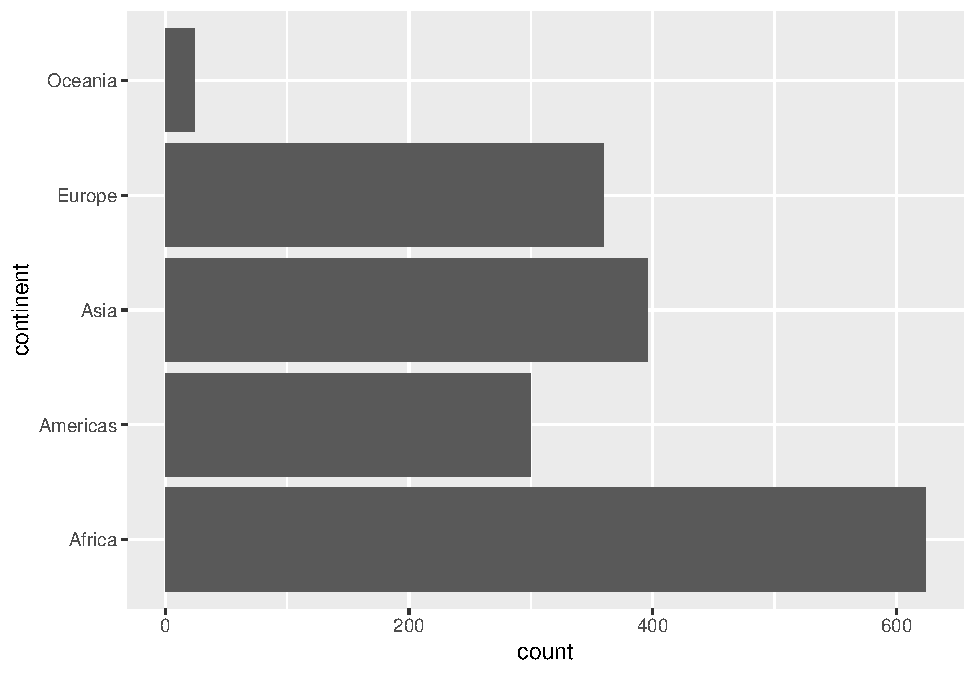
\includegraphics[width=0.49\linewidth]{10_factors_files/figure-latex/unnamed-chunk-9-1} 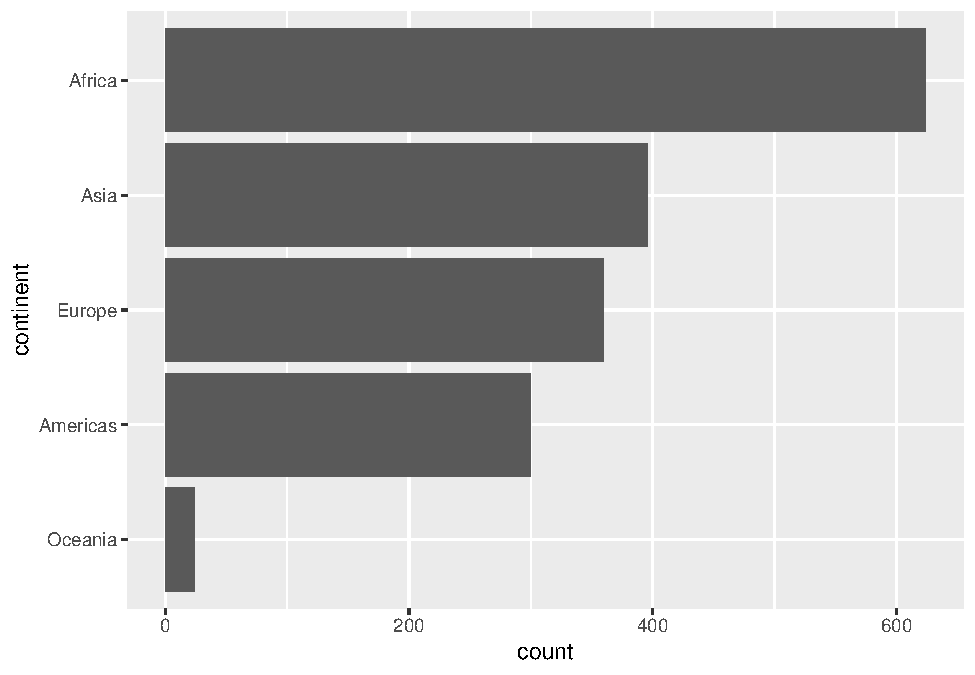
\includegraphics[width=0.49\linewidth]{10_factors_files/figure-latex/unnamed-chunk-9-2}

Now we order \texttt{country} by another variable, forwards and backwards. This other variable is usually quantitative and you will order the factor according to a grouped summary. The factor is the grouping variable and the default summarizing function is \texttt{median()} but you can specify something else.

\begin{Shaded}
\begin{Highlighting}[]
\CommentTok{## order countries by median life expectancy}
\KeywordTok{fct_reorder}\NormalTok{(gapminder}\OperatorTok{$}\NormalTok{country, gapminder}\OperatorTok{$}\NormalTok{lifeExp) }\OperatorTok\StringTok{ }
\StringTok{  }\KeywordTok{levels}\NormalTok{() }\OperatorTok\StringTok{ }\KeywordTok{head}\NormalTok{()}
\CommentTok{#> [1] "Sierra Leone"  "Guinea-Bissau" "Afghanistan"   "Angola"       }
\CommentTok{#> [5] "Somalia"       "Guinea"}

\CommentTok{## order accoring to minimum life exp instead of median}
\KeywordTok{fct_reorder}\NormalTok{(gapminder}\OperatorTok{$}\NormalTok{country, gapminder}\OperatorTok{$}\NormalTok{lifeExp, min) }\OperatorTok\StringTok{ }
\StringTok{  }\KeywordTok{levels}\NormalTok{() }\OperatorTok\StringTok{ }\KeywordTok{head}\NormalTok{()}
\CommentTok{#> [1] "Rwanda"       "Afghanistan"  "Gambia"       "Angola"      }
\CommentTok{#> [5] "Sierra Leone" "Cambodia"}

\CommentTok{## backwards!}
\KeywordTok{fct_reorder}\NormalTok{(gapminder}\OperatorTok{$}\NormalTok{country, gapminder}\OperatorTok{$}\NormalTok{lifeExp, }\DataTypeTok{.desc =} \OtherTok{TRUE}\NormalTok{) }\OperatorTok\StringTok{ }
\StringTok{  }\KeywordTok{levels}\NormalTok{() }\OperatorTok\StringTok{ }\KeywordTok{head}\NormalTok{()}
\CommentTok{#> [1] "Iceland"     "Japan"       "Sweden"      "Switzerland"}
\CommentTok{#> [5] "Netherlands" "Norway"}
\end{Highlighting}
\end{Shaded}

Example of why we reorder factor levels: often makes plots much better! When a factor is mapped to x or y, it should almost always be reordered by the quantitative variable you are mapping to the other one.

Compare the interpretability of these two plots of life expectancy in Asian countries in 2007. The \emph{only difference} is the order of the \texttt{country} factor. Which one do you find easier to learn from?

\begin{Shaded}
\begin{Highlighting}[]
\NormalTok{gap_asia_}\DecValTok{2007}\NormalTok{ <-}\StringTok{ }\NormalTok{gapminder }\OperatorTok\StringTok{ }\KeywordTok{filter}\NormalTok{(year }\OperatorTok{==}\StringTok{ }\DecValTok{2007}\NormalTok{, continent }\OperatorTok{==}\StringTok{ "Asia"}\NormalTok{)}
\KeywordTok{ggplot}\NormalTok{(gap_asia_}\DecValTok{2007}\NormalTok{, }\KeywordTok{aes}\NormalTok{(}\DataTypeTok{x =}\NormalTok{ lifeExp, }\DataTypeTok{y =}\NormalTok{ country)) }\OperatorTok{+}\StringTok{ }\KeywordTok{geom_point}\NormalTok{()}
\KeywordTok{ggplot}\NormalTok{(gap_asia_}\DecValTok{2007}\NormalTok{, }\KeywordTok{aes}\NormalTok{(}\DataTypeTok{x =}\NormalTok{ lifeExp, }\DataTypeTok{y =} \KeywordTok{fct_reorder}\NormalTok{(country, lifeExp))) }\OperatorTok{+}
\StringTok{  }\KeywordTok{geom_point}\NormalTok{()}
\end{Highlighting}
\end{Shaded}

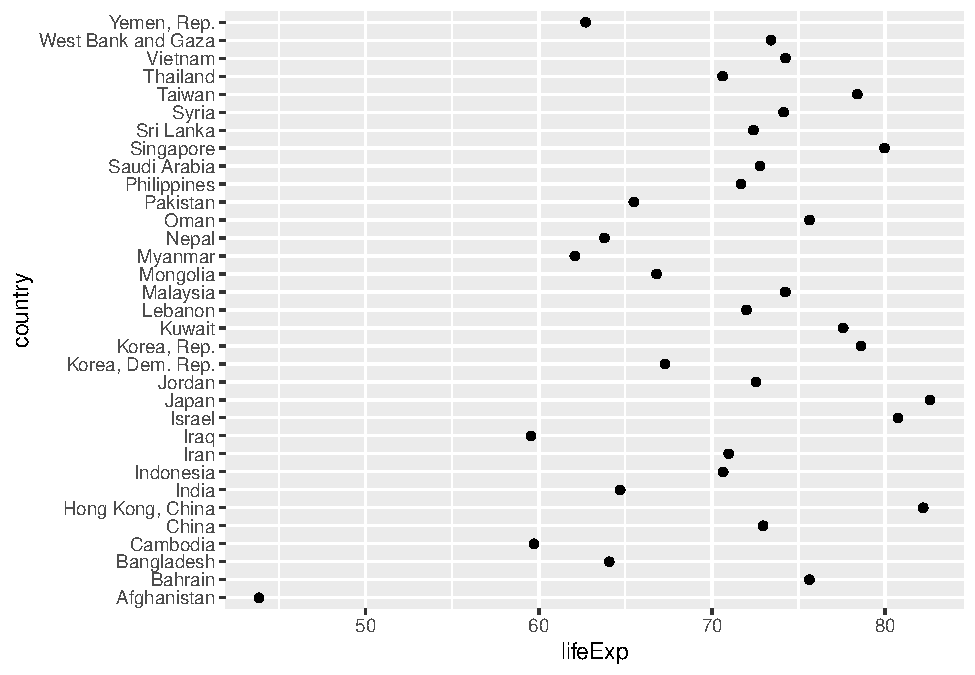
\includegraphics[width=0.49\linewidth]{10_factors_files/figure-latex/alpha-order-silly-1} 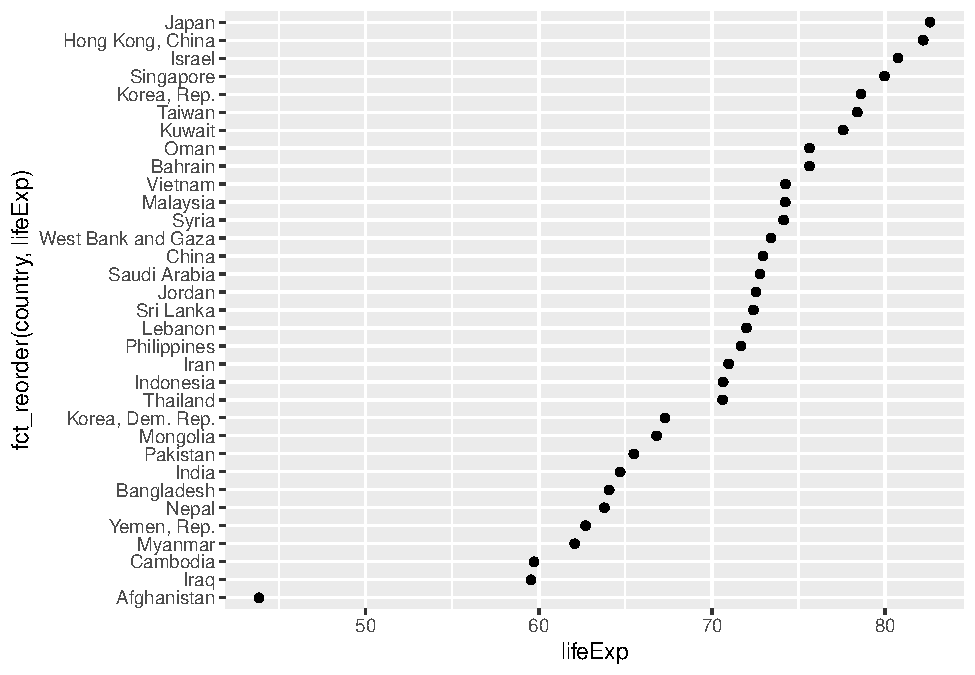
\includegraphics[width=0.49\linewidth]{10_factors_files/figure-latex/alpha-order-silly-2}

Use \texttt{fct\_reorder2()} when you have a line chart of a quantitative x against another quantitative y and your factor provides the color. This way the legend appears in some order as the data! Contrast the legend on the left with the one on the right.

\begin{Shaded}
\begin{Highlighting}[]
\NormalTok{h_countries <-}\StringTok{ }\KeywordTok{c}\NormalTok{(}\StringTok{"Egypt"}\NormalTok{, }\StringTok{"Haiti"}\NormalTok{, }\StringTok{"Romania"}\NormalTok{, }\StringTok{"Thailand"}\NormalTok{, }\StringTok{"Venezuela"}\NormalTok{)}
\NormalTok{h_gap <-}\StringTok{ }\NormalTok{gapminder }\OperatorTok
\StringTok{  }\KeywordTok{filter}\NormalTok{(country }\OperatorTok\StringTok{ }\NormalTok{h_countries) }\OperatorTok\StringTok{ }
\StringTok{  }\KeywordTok{droplevels}\NormalTok{()}
\KeywordTok{ggplot}\NormalTok{(h_gap, }\KeywordTok{aes}\NormalTok{(}\DataTypeTok{x =}\NormalTok{ year, }\DataTypeTok{y =}\NormalTok{ lifeExp, }\DataTypeTok{color =}\NormalTok{ country)) }\OperatorTok{+}
\StringTok{  }\KeywordTok{geom_line}\NormalTok{()}
\KeywordTok{ggplot}\NormalTok{(h_gap, }\KeywordTok{aes}\NormalTok{(}\DataTypeTok{x =}\NormalTok{ year, }\DataTypeTok{y =}\NormalTok{ lifeExp,}
                  \DataTypeTok{color =} \KeywordTok{fct_reorder2}\NormalTok{(country, year, lifeExp))) }\OperatorTok{+}
\StringTok{  }\KeywordTok{geom_line}\NormalTok{() }\OperatorTok{+}
\StringTok{  }\KeywordTok{labs}\NormalTok{(}\DataTypeTok{color =} \StringTok{"country"}\NormalTok{)}
\end{Highlighting}
\end{Shaded}

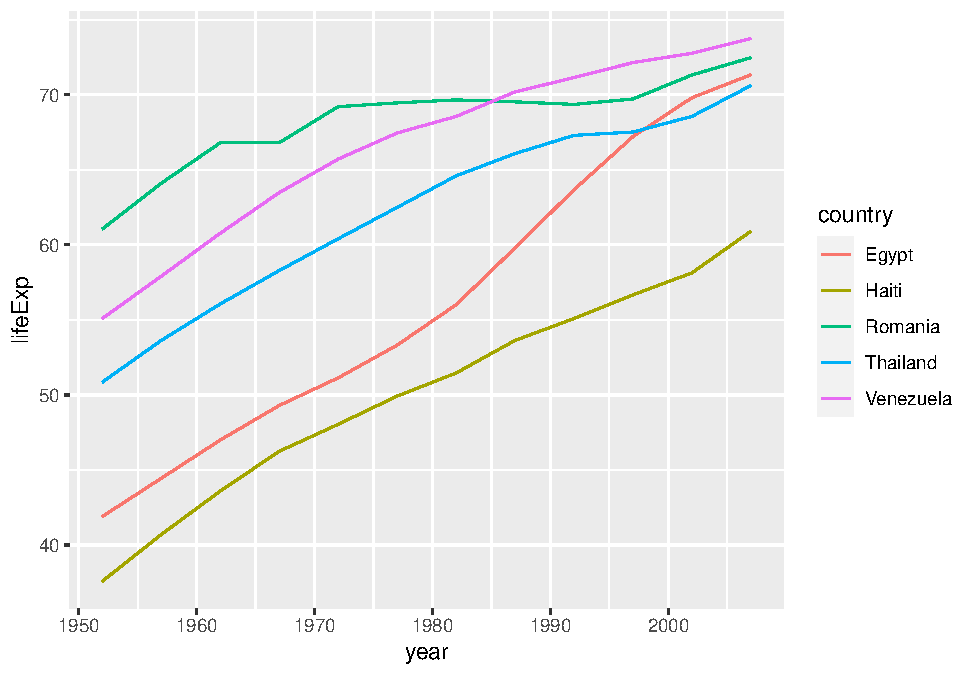
\includegraphics[width=0.49\linewidth]{10_factors_files/figure-latex/legends-made-for-humans-1} 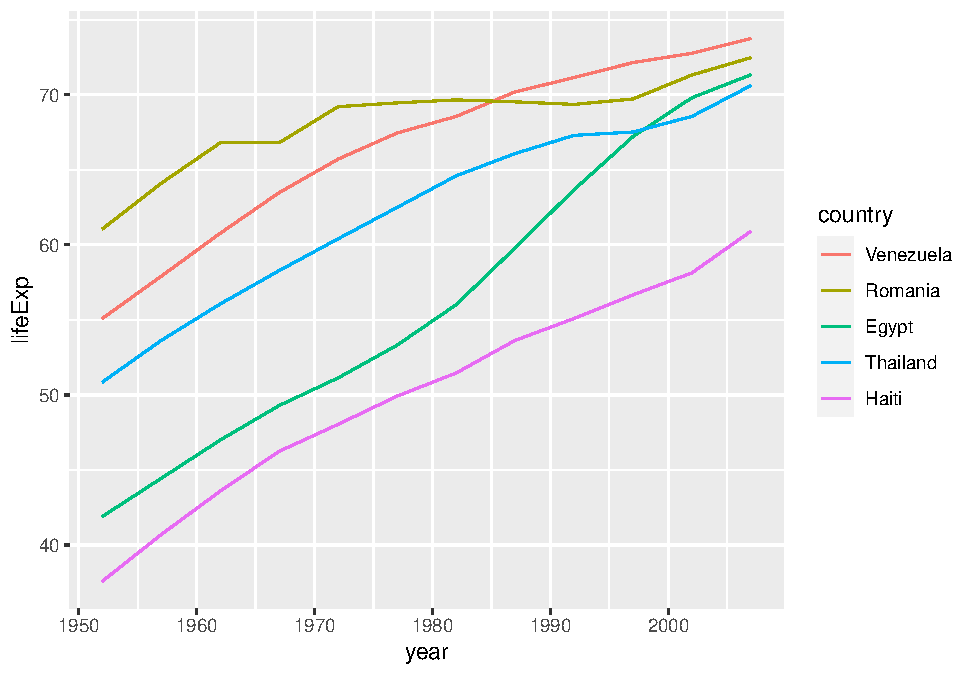
\includegraphics[width=0.49\linewidth]{10_factors_files/figure-latex/legends-made-for-humans-2}

\hypertarget{change-order-of-the-levels-because-i-said-so}{%
\section{Change order of the levels, ``because I said so''}\label{change-order-of-the-levels-because-i-said-so}}

Sometimes you just want to hoist one or more levels to the front. Why? Because I said so. This resembles what we do when we move variables to the front with \texttt{dplyr::select(special\_var,\ everything())}.

\begin{Shaded}
\begin{Highlighting}[]
\NormalTok{h_gap}\OperatorTok{$}\NormalTok{country }\OperatorTok\StringTok{ }\KeywordTok{levels}\NormalTok{()}
\CommentTok{#> [1] "Egypt"     "Haiti"     "Romania"   "Thailand"  "Venezuela"}
\NormalTok{h_gap}\OperatorTok{$}\NormalTok{country }\OperatorTok\StringTok{ }\KeywordTok{fct_relevel}\NormalTok{(}\StringTok{"Romania"}\NormalTok{, }\StringTok{"Haiti"}\NormalTok{) }\OperatorTok\StringTok{ }\KeywordTok{levels}\NormalTok{()}
\CommentTok{#> [1] "Romania"   "Haiti"     "Egypt"     "Thailand"  "Venezuela"}
\end{Highlighting}
\end{Shaded}

This might be useful if you are preparing a report for, say, the Romanian government. The reason for always putting Romania first has nothing to do with the \emph{data}, it is important for external reasons and you need a way to express this.

\hypertarget{recode-the-levels}{%
\section{Recode the levels}\label{recode-the-levels}}

Sometimes you have better ideas about what certain levels should be. This is called recoding.

\begin{Shaded}
\begin{Highlighting}[]
\NormalTok{i_gap <-}\StringTok{ }\NormalTok{gapminder }\OperatorTok\StringTok{ }
\StringTok{  }\KeywordTok{filter}\NormalTok{(country }\OperatorTok\StringTok{ }\KeywordTok{c}\NormalTok{(}\StringTok{"United States"}\NormalTok{, }\StringTok{"Sweden"}\NormalTok{, }\StringTok{"Australia"}\NormalTok{)) }\OperatorTok\StringTok{ }
\StringTok{  }\KeywordTok{droplevels}\NormalTok{()}
\NormalTok{i_gap}\OperatorTok{$}\NormalTok{country }\OperatorTok\StringTok{ }\KeywordTok{levels}\NormalTok{()}
\CommentTok{#> [1] "Australia"     "Sweden"        "United States"}
\NormalTok{i_gap}\OperatorTok{$}\NormalTok{country }\OperatorTok
\StringTok{  }\KeywordTok{fct_recode}\NormalTok{(}\StringTok{"USA"}\NormalTok{ =}\StringTok{ "United States"}\NormalTok{, }\StringTok{"Oz"}\NormalTok{ =}\StringTok{ "Australia"}\NormalTok{) }\OperatorTok\StringTok{ }\KeywordTok{levels}\NormalTok{()}
\CommentTok{#> [1] "Oz"     "Sweden" "USA"}
\end{Highlighting}
\end{Shaded}

\textbf{Exercise:} Isolate the data for \texttt{"Australia"}, \texttt{"Korea,\ Dem.\ Rep."}, and \texttt{"Korea,\ Rep."} in the 2000x. Revalue the country factor levels to \texttt{"Oz"}, \texttt{"North\ Korea"}, and \texttt{"South\ Korea"}.

\hypertarget{grow-a-factor}{%
\section{Grow a factor}\label{grow-a-factor}}

Let's create two data frames, each with data from two countries, dropping unused factor levels.

\begin{Shaded}
\begin{Highlighting}[]
\NormalTok{df1 <-}\StringTok{ }\NormalTok{gapminder }\OperatorTok
\StringTok{  }\KeywordTok{filter}\NormalTok{(country }\OperatorTok\StringTok{ }\KeywordTok{c}\NormalTok{(}\StringTok{"United States"}\NormalTok{, }\StringTok{"Mexico"}\NormalTok{), year }\OperatorTok{>}\StringTok{ }\DecValTok{2000}\NormalTok{) }\OperatorTok
\StringTok{  }\KeywordTok{droplevels}\NormalTok{()}
\NormalTok{df2 <-}\StringTok{ }\NormalTok{gapminder }\OperatorTok
\StringTok{  }\KeywordTok{filter}\NormalTok{(country }\OperatorTok\StringTok{ }\KeywordTok{c}\NormalTok{(}\StringTok{"France"}\NormalTok{, }\StringTok{"Germany"}\NormalTok{), year }\OperatorTok{>}\StringTok{ }\DecValTok{2000}\NormalTok{) }\OperatorTok
\StringTok{  }\KeywordTok{droplevels}\NormalTok{()}
\end{Highlighting}
\end{Shaded}

The \texttt{country} factors in \texttt{df1} and \texttt{df2} have different levels.

\begin{Shaded}
\begin{Highlighting}[]
\KeywordTok{levels}\NormalTok{(df1}\OperatorTok{$}\NormalTok{country)}
\CommentTok{#> [1] "Mexico"        "United States"}
\KeywordTok{levels}\NormalTok{(df2}\OperatorTok{$}\NormalTok{country)}
\CommentTok{#> [1] "France"  "Germany"}
\end{Highlighting}
\end{Shaded}

Can you just combine them?

\begin{Shaded}
\begin{Highlighting}[]
\KeywordTok{c}\NormalTok{(df1}\OperatorTok{$}\NormalTok{country, df2}\OperatorTok{$}\NormalTok{country)}
\CommentTok{#> [1] 1 1 2 2 1 1 2 2}
\end{Highlighting}
\end{Shaded}

Umm, no. That is wrong on many levels! Use \texttt{fct\_c()} to do this.

\begin{Shaded}
\begin{Highlighting}[]
\KeywordTok{fct_c}\NormalTok{(df1}\OperatorTok{$}\NormalTok{country, df2}\OperatorTok{$}\NormalTok{country)}
\CommentTok{#> [1] Mexico        Mexico        United States United States}
\CommentTok{#> [5] France        France        Germany       Germany      }
\CommentTok{#> Levels: Mexico United States France Germany}
\end{Highlighting}
\end{Shaded}

\textbf{Exercise:} Explore how different forms of row binding work behave here, in terms of the \texttt{country} variable in the result.

\begin{Shaded}
\begin{Highlighting}[]
\KeywordTok{bind_rows}\NormalTok{(df1, df2)}
\CommentTok{#> # A tibble: 8 x 6}
\CommentTok{#>   country       continent  year lifeExp       pop gdpPercap}
\CommentTok{#>   <fct>         <fct>     <int>   <dbl>     <int>     <dbl>}
\CommentTok{#> 1 Mexico        Americas   2002    74.9 102479927    10742.}
\CommentTok{#> 2 Mexico        Americas   2007    76.2 108700891    11978.}
\CommentTok{#> 3 United States Americas   2002    77.3 287675526    39097.}
\CommentTok{#> 4 United States Americas   2007    78.2 301139947    42952.}
\CommentTok{#> 5 France        Europe     2002    79.6  59925035    28926.}
\CommentTok{#> 6 France        Europe     2007    80.7  61083916    30470.}
\CommentTok{#> 7 Germany       Europe     2002    78.7  82350671    30036.}
\CommentTok{#> 8 Germany       Europe     2007    79.4  82400996    32170.}
\KeywordTok{rbind}\NormalTok{(df1, df2)}
\CommentTok{#> # A tibble: 8 x 6}
\CommentTok{#>   country       continent  year lifeExp       pop gdpPercap}
\CommentTok{#>   <fct>         <fct>     <int>   <dbl>     <int>     <dbl>}
\CommentTok{#> 1 Mexico        Americas   2002    74.9 102479927    10742.}
\CommentTok{#> 2 Mexico        Americas   2007    76.2 108700891    11978.}
\CommentTok{#> 3 United States Americas   2002    77.3 287675526    39097.}
\CommentTok{#> 4 United States Americas   2007    78.2 301139947    42952.}
\CommentTok{#> 5 France        Europe     2002    79.6  59925035    28926.}
\CommentTok{#> 6 France        Europe     2007    80.7  61083916    30470.}
\CommentTok{#> 7 Germany       Europe     2002    78.7  82350671    30036.}
\CommentTok{#> 8 Germany       Europe     2007    79.4  82400996    32170.}
\end{Highlighting}
\end{Shaded}

\hypertarget{character-vectors}{%
\chapter{Character vectors}\label{character-vectors}}

\hypertarget{character-vectors-where-they-fit-in}{%
\section{Character vectors: where they fit in}\label{character-vectors-where-they-fit-in}}

We've spent a lot of time working with big, beautiful data frames. That are clean and wholesome, like the Gapminder data.

But real life will be much nastier. You will bring data into R from the outside world and discover there are problems. You might think: how hard can it be to deal with character data? And the answer is: it can be very hard!

\begin{itemize}
\tightlist
\item
  \href{https://stackstatus.net/post/147710624694/outage-postmortem-july-20-2016}{Stack Exchange outage}
\item
  \href{https://emailregex.com}{Regexes to validate/match email addresses}
\item
  \href{https://davidvgalbraith.com/how-i-fixed-atom/}{Fixing an Atom bug}
\end{itemize}

Here we discuss common remedial tasks for cleaning and transforming character data, also known as ``strings''. A data frame or tibble will consist of one or more \emph{atomic vectors} of a certain class. This lesson deals with things you can do with vectors of class \texttt{character}.

\hypertarget{resources}{%
\section{Resources}\label{resources}}

I start with this because we cannot possibly do this topic justice in a short amount of time. Our goal is to make you aware of broad classes of problems and their respective solutions. Once you have a character problem in real life, these resources will be extremely helpful as you delve deeper.

\hypertarget{manipulating-character-vectors}{%
\subsection{Manipulating character vectors}\label{manipulating-character-vectors}}

\begin{itemize}
\tightlist
\item
  \href{https://stringr.tidyverse.org}{stringr} package.

  \begin{itemize}
  \tightlist
  \item
    A core package in the \href{https://tidyverse.tidyverse.org}{tidyverse}. It is installed via \texttt{install.packages("tidyverse")} and also loaded via \texttt{library(tidyverse)}. Of course, you can also install or load it individually.
  \item
    Main functions start with \texttt{str\_}. Auto-complete is your friend.
  \item
    Replacements for base functions re: string manipulation and regular expressions (see below).
  \item
    Main advantages over base functions: greater consistency about inputs and outputs. Outputs are more ready for your next analytical task.
  \end{itemize}
\item
  \href{https://tidyr.tidyverse.org}{tidyr} package.

  \begin{itemize}
  \tightlist
  \item
    Especially useful for functions that split one character vector into many and \emph{vice versa}: \texttt{separate()}, \texttt{unite()}, \texttt{extract()}.
  \end{itemize}
\item
  Base functions: \texttt{nchar()}, \texttt{strsplit()}, \texttt{substr()}, \texttt{paste()}, \texttt{paste0()}.
\item
  The \href{https://glue.tidyverse.org}{glue} package is fantastic for string interpolation. If \texttt{stringr::str\_interp()} doesn't get your job done, check out the glue package.
\end{itemize}

\hypertarget{regular-expressions-resources}{%
\subsection{Regular expressions resources}\label{regular-expressions-resources}}

A God-awful and powerful language for expressing patterns to match in text or for search-and-replace. Frequently described as ``write only'', because regular expressions are easier to write than to read/understand. And they are not particularly easy to write.

\begin{itemize}
\tightlist
\item
  We again prefer the \href{https://stringr.tidyverse.org}{stringr} package over base functions. Why?

  \begin{itemize}
  \tightlist
  \item
    Wraps \href{http://www.gagolewski.com/software/stringi/}{stringi}, which is a great place to look if stringr isn't powerful enough.
  \item
    Standardized on \href{http://userguide.icu-project.org/strings/regexp}{ICU regular expressions}, so you can stop toggling \texttt{perl\ =\ TRUE/FALSE} at random.
  \item
    Results come back in a form that is much friendlier for downstream work.
  \end{itemize}
\item
  The \href{https://r4ds.had.co.nz/strings.html}{Strings chapter} of \href{https://r4ds.had.co.nz}{R for Data Science} \citep{wickham2016} is a great resource.
\item
  Older STAT 545 lessons on regular expressions have some excellent content. This lesson draws on them, but makes more rigorous use of stringr and uses example data that is easier to support long-term.

  \begin{itemize}
  \tightlist
  \item
    \protect\hyperlink{oldies}{2014 Intro to regular expressions} by TA Gloria Li (Appendix \ref{oldies}).
  \item
    \protect\hyperlink{oldies}{2015 Regular expressions and character data in R} by TA Kieran Samuk (Appendix \ref{oldies}).
  \end{itemize}
\item
  \href{https://github.com/rstudio/cheatsheets/raw/master/regex.pdf}{Regular Expressions in R Cheat Sheet} by Ian Kopacka.
\item
  Regex testers:

  \begin{itemize}
  \tightlist
  \item
    \href{https://regex101.com}{regex101.com}
  \item
    \href{https://regexr.com}{regexr.com}
  \end{itemize}
\item
  \href{https://github.com/kevinushey/rex}{rex} R package: make regular expression from human readable expressions.
\item
  Base functions: \texttt{grep()} and friends.
\end{itemize}

\hypertarget{character-encoding-resources}{%
\subsection{Character encoding resources}\label{character-encoding-resources}}

\begin{itemize}
\tightlist
\item
  \href{https://r4ds.had.co.nz/data-import.html\#readr-strings}{Strings subsection of data import chapter} in \href{https://r4ds.had.co.nz}{R for Data Science} \citep{wickham2016}.
\item
  Screeds on the Minimum Everyone Needs to Know about encoding:

  \begin{itemize}
  \tightlist
  \item
    \href{https://www.joelonsoftware.com/2003/10/08/the-absolute-minimum-every-software-developer-absolutely-positively-must-know-about-unicode-and-character-sets-no-excuses/}{``The Absolute Minimum Every Software Developer Absolutely, Positively Must Know About Unicode and Character Sets (No Excuses!)''}
  \item
    \href{http://kunststube.net/encoding/}{``What Every Programmer Absolutely, Positively Needs To Know About Encodings And Character Sets To Work With Text''}
  \end{itemize}
\item
  Chapter \ref{character-encoding} - I've translated this blog post, \href{https://www.justinweiss.com/articles/3-steps-to-fix-encoding-problems-in-ruby/}{``3 Steps to Fix Encoding Problems in Ruby''}, into R as the first step to developing a lesson.
\end{itemize}

\hypertarget{character-vectors-that-live-in-a-data-frame}{%
\subsection{Character vectors that live in a data frame}\label{character-vectors-that-live-in-a-data-frame}}

\begin{itemize}
\tightlist
\item
  Certain operations are facilitated by tidyr. These are described below.
\item
  For a general discussion of how to work on variables that live in a data frame, see \protect\hyperlink{oldies}{Vectors versus tibbles} (Appendix \ref{oldies}).
\end{itemize}

\hypertarget{load-the-tidyverse-which-includes-stringr}{%
\section{Load the tidyverse, which includes stringr}\label{load-the-tidyverse-which-includes-stringr}}

\begin{Shaded}
\begin{Highlighting}[]
\KeywordTok{library}\NormalTok{(tidyverse)}
\CommentTok{#> ── Attaching packages ──────────────────────────── tidyverse 1.3.0 ──}
\CommentTok{#> ✓ ggplot2 3.3.2     ✓ purrr   0.3.4}
\CommentTok{#> ✓ tibble  3.0.3     ✓ dplyr   1.0.2}
\CommentTok{#> ✓ tidyr   1.1.2     ✓ stringr 1.4.0}
\CommentTok{#> ✓ readr   1.3.1     ✓ forcats 0.5.0}
\CommentTok{#> ── Conflicts ─────────────────────────────── tidyverse_conflicts() ──}
\CommentTok{#> x dplyr::filter() masks stats::filter()}
\CommentTok{#> x dplyr::lag()    masks stats::lag()}
\end{Highlighting}
\end{Shaded}

\hypertarget{regex-free-string-manipulation-with-stringr-and-tidyr}{%
\section{Regex-free string manipulation with stringr and tidyr}\label{regex-free-string-manipulation-with-stringr-and-tidyr}}

Basic string manipulation tasks:

\begin{itemize}
\tightlist
\item
  Study a single character vector

  \begin{itemize}
  \tightlist
  \item
    How long are the strings?
  \item
    Presence/absence of a literal string
  \end{itemize}
\item
  Operate on a single character vector

  \begin{itemize}
  \tightlist
  \item
    Keep/discard elements that contain a literal string
  \item
    Split into two or more character vectors using a fixed delimiter\\
  \item
    Snip out pieces of the strings based on character position
  \item
    Collapse into a single string
  \end{itemize}
\item
  Operate on two or more character vectors

  \begin{itemize}
  \tightlist
  \item
    Glue them together element-wise to get a new character vector.
  \end{itemize}
\end{itemize}

\emph{\texttt{fruit}, \texttt{words}, and \texttt{sentences} are character vectors that ship with stringr for practicing.}

\hypertarget{detect-or-filter-on-a-target-string}{%
\subsection{Detect or filter on a target string}\label{detect-or-filter-on-a-target-string}}

Determine presence/absence of a literal string with \texttt{str\_detect()}. Spoiler: later we see \texttt{str\_detect()} also detects regular expressions.

Which fruits actually use the word ``fruit''?

\begin{Shaded}
\begin{Highlighting}[]
\KeywordTok{str_detect}\NormalTok{(fruit, }\DataTypeTok{pattern =} \StringTok{"fruit"}\NormalTok{)}
\CommentTok{#>  [1] FALSE FALSE FALSE FALSE FALSE FALSE FALSE FALSE FALSE FALSE}
\CommentTok{#> [11] FALSE  TRUE FALSE FALSE FALSE FALSE FALSE FALSE FALSE FALSE}
\CommentTok{#> [21] FALSE FALSE FALSE FALSE FALSE  TRUE FALSE FALSE FALSE FALSE}
\CommentTok{#> [31] FALSE FALSE FALSE FALSE  TRUE FALSE FALSE FALSE  TRUE FALSE}
\CommentTok{#> [41] FALSE  TRUE FALSE FALSE FALSE FALSE FALSE FALSE FALSE FALSE}
\CommentTok{#> [51] FALSE FALSE FALSE FALSE FALSE FALSE  TRUE FALSE FALSE FALSE}
\CommentTok{#> [61] FALSE FALSE FALSE FALSE FALSE FALSE FALSE FALSE FALSE FALSE}
\CommentTok{#> [71] FALSE FALSE FALSE FALSE  TRUE FALSE FALSE FALSE  TRUE FALSE}
\end{Highlighting}
\end{Shaded}

What's the easiest way to get the actual fruits that match? Use \texttt{str\_subset()} to keep only the matching elements. Note we are storing this new vector \texttt{my\_fruit} to use in later examples!

\begin{Shaded}
\begin{Highlighting}[]
\NormalTok{(my_fruit <-}\StringTok{ }\KeywordTok{str_subset}\NormalTok{(fruit, }\DataTypeTok{pattern =} \StringTok{"fruit"}\NormalTok{))}
\CommentTok{#> [1] "breadfruit"   "dragonfruit"  "grapefruit"   "jackfruit"   }
\CommentTok{#> [5] "kiwi fruit"   "passionfruit" "star fruit"   "ugli fruit"}
\end{Highlighting}
\end{Shaded}

\hypertarget{string-splitting-by-delimiter}{%
\subsection{String splitting by delimiter}\label{string-splitting-by-delimiter}}

Use \texttt{stringr::str\_split()} to split strings on a delimiter. Some of our fruits are compound words, like ``grapefruit'', but some have two words, like ``ugli fruit''. Here we split on a single space \texttt{"\ "}, but show use of a regular expression later.

\begin{Shaded}
\begin{Highlighting}[]
\KeywordTok{str_split}\NormalTok{(my_fruit, }\DataTypeTok{pattern =} \StringTok{" "}\NormalTok{)}
\CommentTok{#> [[1]]}
\CommentTok{#> [1] "breadfruit"}
\CommentTok{#> }
\CommentTok{#> [[2]]}
\CommentTok{#> [1] "dragonfruit"}
\CommentTok{#> }
\CommentTok{#> [[3]]}
\CommentTok{#> [1] "grapefruit"}
\CommentTok{#> }
\CommentTok{#> [[4]]}
\CommentTok{#> [1] "jackfruit"}
\CommentTok{#> }
\CommentTok{#> [[5]]}
\CommentTok{#> [1] "kiwi"  "fruit"}
\CommentTok{#> }
\CommentTok{#> [[6]]}
\CommentTok{#> [1] "passionfruit"}
\CommentTok{#> }
\CommentTok{#> [[7]]}
\CommentTok{#> [1] "star"  "fruit"}
\CommentTok{#> }
\CommentTok{#> [[8]]}
\CommentTok{#> [1] "ugli"  "fruit"}
\end{Highlighting}
\end{Shaded}

It's bummer that we get a \emph{list} back. But it must be so! In full generality, split strings must return list, because who knows how many pieces there will be?

If you are willing to commit to the number of pieces, you can use \texttt{str\_split\_fixed()} and get a character matrix. You're welcome!

\begin{Shaded}
\begin{Highlighting}[]
\KeywordTok{str_split_fixed}\NormalTok{(my_fruit, }\DataTypeTok{pattern =} \StringTok{" "}\NormalTok{, }\DataTypeTok{n =} \DecValTok{2}\NormalTok{)}
\CommentTok{#>      [,1]           [,2]   }
\CommentTok{#> [1,] "breadfruit"   ""     }
\CommentTok{#> [2,] "dragonfruit"  ""     }
\CommentTok{#> [3,] "grapefruit"   ""     }
\CommentTok{#> [4,] "jackfruit"    ""     }
\CommentTok{#> [5,] "kiwi"         "fruit"}
\CommentTok{#> [6,] "passionfruit" ""     }
\CommentTok{#> [7,] "star"         "fruit"}
\CommentTok{#> [8,] "ugli"         "fruit"}
\end{Highlighting}
\end{Shaded}

If the to-be-split variable lives in a data frame, \texttt{tidyr::separate()} will split it into 2 or more variables.

\begin{Shaded}
\begin{Highlighting}[]
\NormalTok{my_fruit_df <-}\StringTok{ }\KeywordTok{tibble}\NormalTok{(my_fruit)}
\NormalTok{my_fruit_df }\OperatorTok\StringTok{ }
\StringTok{  }\KeywordTok{separate}\NormalTok{(my_fruit, }\DataTypeTok{into =} \KeywordTok{c}\NormalTok{(}\StringTok{"pre"}\NormalTok{, }\StringTok{"post"}\NormalTok{), }\DataTypeTok{sep =} \StringTok{" "}\NormalTok{)}
\CommentTok{#> Warning: Expected 2 pieces. Missing pieces filled with `NA` in 5 rows}
\CommentTok{#> [1, 2, 3, 4, 6].}
\CommentTok{#> # A tibble: 8 x 2}
\CommentTok{#>   pre          post }
\CommentTok{#>   <chr>        <chr>}
\CommentTok{#> 1 breadfruit   <NA> }
\CommentTok{#> 2 dragonfruit  <NA> }
\CommentTok{#> 3 grapefruit   <NA> }
\CommentTok{#> 4 jackfruit    <NA> }
\CommentTok{#> 5 kiwi         fruit}
\CommentTok{#> 6 passionfruit <NA> }
\CommentTok{#> 7 star         fruit}
\CommentTok{#> 8 ugli         fruit}
\end{Highlighting}
\end{Shaded}

\hypertarget{substring-extraction-and-replacement-by-position}{%
\subsection{Substring extraction (and replacement) by position}\label{substring-extraction-and-replacement-by-position}}

Count characters in your strings with \texttt{str\_length()}. Note this is different from the length of the character vector itself.

\begin{Shaded}
\begin{Highlighting}[]
\KeywordTok{length}\NormalTok{(my_fruit)}
\CommentTok{#> [1] 8}
\KeywordTok{str_length}\NormalTok{(my_fruit)}
\CommentTok{#> [1] 10 11 10  9 10 12 10 10}
\end{Highlighting}
\end{Shaded}

You can snip out substrings based on character position with \texttt{str\_sub()}.

\begin{Shaded}
\begin{Highlighting}[]
\KeywordTok{head}\NormalTok{(fruit) }\OperatorTok\StringTok{ }
\StringTok{  }\KeywordTok{str_sub}\NormalTok{(}\DecValTok{1}\NormalTok{, }\DecValTok{3}\NormalTok{)}
\CommentTok{#> [1] "app" "apr" "avo" "ban" "bel" "bil"}
\end{Highlighting}
\end{Shaded}

The \texttt{start} and \texttt{end} arguments are vectorised. Example: a sliding 3-character window.

\begin{Shaded}
\begin{Highlighting}[]
\KeywordTok{tibble}\NormalTok{(fruit) }\OperatorTok\StringTok{ }
\StringTok{  }\KeywordTok{head}\NormalTok{() }\OperatorTok\StringTok{ }
\StringTok{  }\KeywordTok{mutate}\NormalTok{(}\DataTypeTok{snip =} \KeywordTok{str_sub}\NormalTok{(fruit, }\DecValTok{1}\OperatorTok{:}\DecValTok{6}\NormalTok{, }\DecValTok{3}\OperatorTok{:}\DecValTok{8}\NormalTok{))}
\CommentTok{#> # A tibble: 6 x 2}
\CommentTok{#>   fruit       snip }
\CommentTok{#>   <chr>       <chr>}
\CommentTok{#> 1 apple       "app"}
\CommentTok{#> 2 apricot     "pri"}
\CommentTok{#> 3 avocado     "oca"}
\CommentTok{#> 4 banana      "ana"}
\CommentTok{#> 5 bell pepper " pe"}
\CommentTok{#> 6 bilberry    "rry"}
\end{Highlighting}
\end{Shaded}

Finally, \texttt{str\_sub()} also works for assignment, i.e.~on the left hand side of \texttt{\textless{}-}.

\begin{Shaded}
\begin{Highlighting}[]
\NormalTok{(x <-}\StringTok{ }\KeywordTok{head}\NormalTok{(fruit, }\DecValTok{3}\NormalTok{))}
\CommentTok{#> [1] "apple"   "apricot" "avocado"}
\KeywordTok{str_sub}\NormalTok{(x, }\DecValTok{1}\NormalTok{, }\DecValTok{3}\NormalTok{) <-}\StringTok{ "AAA"}
\NormalTok{x}
\CommentTok{#> [1] "AAAle"   "AAAicot" "AAAcado"}
\end{Highlighting}
\end{Shaded}

\hypertarget{collapse-a-vector}{%
\subsection{Collapse a vector}\label{collapse-a-vector}}

You can collapse a character vector of length \texttt{n\ \textgreater{}\ 1} to a single string with \texttt{str\_c()}, which also has other uses (see the \protect\hyperlink{catenate-vectors}{following section}).

\begin{Shaded}
\begin{Highlighting}[]
\KeywordTok{head}\NormalTok{(fruit) }\OperatorTok\StringTok{ }
\StringTok{  }\KeywordTok{str_c}\NormalTok{(}\DataTypeTok{collapse =} \StringTok{", "}\NormalTok{)}
\CommentTok{#> [1] "apple, apricot, avocado, banana, bell pepper, bilberry"}
\end{Highlighting}
\end{Shaded}

\hypertarget{catenate-vectors}{%
\subsection{Create a character vector by catenating multiple vectors}\label{catenate-vectors}}

If you have two or more character vectors of the same length, you can glue them together element-wise, to get a new vector of that length. Here are some \ldots{} awful smoothie flavors?

\begin{Shaded}
\begin{Highlighting}[]
\KeywordTok{str_c}\NormalTok{(fruit[}\DecValTok{1}\OperatorTok{:}\DecValTok{4}\NormalTok{], fruit[}\DecValTok{5}\OperatorTok{:}\DecValTok{8}\NormalTok{], }\DataTypeTok{sep =} \StringTok{" & "}\NormalTok{)}
\CommentTok{#> [1] "apple & bell pepper"   "apricot & bilberry"   }
\CommentTok{#> [3] "avocado & blackberry"  "banana & blackcurrant"}
\end{Highlighting}
\end{Shaded}

Element-wise catenation can be combined with collapsing.

\begin{Shaded}
\begin{Highlighting}[]
\KeywordTok{str_c}\NormalTok{(fruit[}\DecValTok{1}\OperatorTok{:}\DecValTok{4}\NormalTok{], fruit[}\DecValTok{5}\OperatorTok{:}\DecValTok{8}\NormalTok{], }\DataTypeTok{sep =} \StringTok{" & "}\NormalTok{, }\DataTypeTok{collapse =} \StringTok{", "}\NormalTok{)}
\CommentTok{#> [1] "apple & bell pepper, apricot & bilberry, avocado & blackberry, banana & blackcurrant"}
\end{Highlighting}
\end{Shaded}

If the to-be-combined vectors are variables in a data frame, you can use \texttt{tidyr::unite()} to make a single new variable from them.

\begin{Shaded}
\begin{Highlighting}[]
\NormalTok{fruit_df <-}\StringTok{ }\KeywordTok{tibble}\NormalTok{(}
  \DataTypeTok{fruit1 =}\NormalTok{ fruit[}\DecValTok{1}\OperatorTok{:}\DecValTok{4}\NormalTok{],}
  \DataTypeTok{fruit2 =}\NormalTok{ fruit[}\DecValTok{5}\OperatorTok{:}\DecValTok{8}\NormalTok{]}
\NormalTok{)}
\NormalTok{fruit_df }\OperatorTok\StringTok{ }
\StringTok{  }\KeywordTok{unite}\NormalTok{(}\StringTok{"flavor_combo"}\NormalTok{, fruit1, fruit2, }\DataTypeTok{sep =} \StringTok{" & "}\NormalTok{)}
\CommentTok{#> # A tibble: 4 x 1}
\CommentTok{#>   flavor_combo         }
\CommentTok{#>   <chr>                }
\CommentTok{#> 1 apple & bell pepper  }
\CommentTok{#> 2 apricot & bilberry   }
\CommentTok{#> 3 avocado & blackberry }
\CommentTok{#> 4 banana & blackcurrant}
\end{Highlighting}
\end{Shaded}

\hypertarget{substring-replacement}{%
\subsection{Substring replacement}\label{substring-replacement}}

You can replace a pattern with \texttt{str\_replace()}. Here we use an explicit string-to-replace, but later we revisit with a regular expression.

\begin{Shaded}
\begin{Highlighting}[]
\KeywordTok{str_replace}\NormalTok{(my_fruit, }\DataTypeTok{pattern =} \StringTok{"fruit"}\NormalTok{, }\DataTypeTok{replacement =} \StringTok{"THINGY"}\NormalTok{)}
\CommentTok{#> [1] "breadTHINGY"   "dragonTHINGY"  "grapeTHINGY"   "jackTHINGY"   }
\CommentTok{#> [5] "kiwi THINGY"   "passionTHINGY" "star THINGY"   "ugli THINGY"}
\end{Highlighting}
\end{Shaded}

A special case that comes up a lot is replacing \texttt{NA}, for which there is \texttt{str\_replace\_na()}.

\begin{Shaded}
\begin{Highlighting}[]
\NormalTok{melons <-}\StringTok{ }\KeywordTok{str_subset}\NormalTok{(fruit, }\DataTypeTok{pattern =} \StringTok{"melon"}\NormalTok{)}
\NormalTok{melons[}\DecValTok{2}\NormalTok{] <-}\StringTok{ }\OtherTok{NA}
\NormalTok{melons}
\CommentTok{#> [1] "canary melon" NA             "watermelon"}
\KeywordTok{str_replace_na}\NormalTok{(melons, }\StringTok{"UNKNOWN MELON"}\NormalTok{)}
\CommentTok{#> [1] "canary melon"  "UNKNOWN MELON" "watermelon"}
\end{Highlighting}
\end{Shaded}

If the \texttt{NA}-afflicted variable lives in a data frame, you can use \texttt{tidyr::replace\_na()}.

\begin{Shaded}
\begin{Highlighting}[]
\KeywordTok{tibble}\NormalTok{(melons) }\OperatorTok\StringTok{ }
\StringTok{  }\KeywordTok{replace_na}\NormalTok{(}\DataTypeTok{replace =} \KeywordTok{list}\NormalTok{(}\DataTypeTok{melons =} \StringTok{"UNKNOWN MELON"}\NormalTok{))}
\CommentTok{#> # A tibble: 3 x 1}
\CommentTok{#>   melons       }
\CommentTok{#>   <chr>        }
\CommentTok{#> 1 canary melon }
\CommentTok{#> 2 UNKNOWN MELON}
\CommentTok{#> 3 watermelon}
\end{Highlighting}
\end{Shaded}

And that concludes our treatment of regex-free manipulations of character data!

\hypertarget{regular-expressions-with-stringr}{%
\section{Regular expressions with stringr}\label{regular-expressions-with-stringr}}

\begin{figure}

\includegraphics[width=0.5\linewidth]{img/regexbytrialanderror-big-smaller} \caption{From [\@ThePracticalDev](https://twitter.com/ThePracticalDev/status/774309983467016193)}\label{fig:unnamed-chunk-18}
\end{figure}

\hypertarget{load-gapminder}{%
\subsection{Load gapminder}\label{load-gapminder}}

The country names in the \texttt{gapminder} data frame are convenient for examples. Load it now and store the 142 unique country names to the object \texttt{countries}.

\begin{Shaded}
\begin{Highlighting}[]
\KeywordTok{library}\NormalTok{(gapminder)}
\NormalTok{countries <-}\StringTok{ }\KeywordTok{levels}\NormalTok{(gapminder}\OperatorTok{$}\NormalTok{country)}
\end{Highlighting}
\end{Shaded}

\hypertarget{characters-with-special-meaning}{%
\subsection{Characters with special meaning}\label{characters-with-special-meaning}}

Frequently your string tasks cannot be expressed in terms of a fixed string, but can be described in terms of a \textbf{pattern}. Regular expressions, a.k.a ``regexes'', are the standard way to specify these patterns. In regexes, specific characters and constructs take on special meaning in order to match multiple strings.

The first metacharacter is the period \texttt{.}, which stands for any single character, except a newline (which by the way, is represented by \texttt{\textbackslash{}n}). The regex \texttt{a.b} will match all countries that have an \texttt{a}, followed by any single character, followed by \texttt{b}. Yes, regexes are case sensitive, i.e.~``Italy'' does not match.

\begin{Shaded}
\begin{Highlighting}[]
\KeywordTok{str_subset}\NormalTok{(countries, }\DataTypeTok{pattern =} \StringTok{"i.a"}\NormalTok{)}
\CommentTok{#>  [1] "Argentina"                "Bosnia and Herzegovina"  }
\CommentTok{#>  [3] "Burkina Faso"             "Central African Republic"}
\CommentTok{#>  [5] "China"                    "Costa Rica"              }
\CommentTok{#>  [7] "Dominican Republic"       "Hong Kong, China"        }
\CommentTok{#>  [9] "Jamaica"                  "Mauritania"              }
\CommentTok{#> [11] "Nicaragua"                "South Africa"            }
\CommentTok{#> [13] "Swaziland"                "Taiwan"                  }
\CommentTok{#> [15] "Thailand"                 "Trinidad and Tobago"}
\end{Highlighting}
\end{Shaded}

Notice that \texttt{i.a} matches ``ina'', ``ica'', ``ita'', and more.

\textbf{Anchors} can be included to express where the expression must occur within the string. The \texttt{\^{}} indicates the beginning of string and \texttt{\$} indicates the end.

Note how the regex \texttt{i.a\$} matches many fewer countries than \texttt{i.a} alone. Likewise, more elements of \texttt{my\_fruit} match \texttt{d} than \texttt{\^{}d}, which requires ``d'' at string start.

\begin{Shaded}
\begin{Highlighting}[]
\KeywordTok{str_subset}\NormalTok{(countries, }\DataTypeTok{pattern =} \StringTok{"i.a$"}\NormalTok{)}
\CommentTok{#> [1] "Argentina"              "Bosnia and Herzegovina"}
\CommentTok{#> [3] "China"                  "Costa Rica"            }
\CommentTok{#> [5] "Hong Kong, China"       "Jamaica"               }
\CommentTok{#> [7] "South Africa"}
\KeywordTok{str_subset}\NormalTok{(my_fruit, }\DataTypeTok{pattern =} \StringTok{"d"}\NormalTok{)}
\CommentTok{#> [1] "breadfruit"  "dragonfruit"}
\KeywordTok{str_subset}\NormalTok{(my_fruit, }\DataTypeTok{pattern =} \StringTok{"^d"}\NormalTok{)}
\CommentTok{#> [1] "dragonfruit"}
\end{Highlighting}
\end{Shaded}

The metacharacter \texttt{\textbackslash{}b} indicates a \textbf{word boundary} and \texttt{\textbackslash{}B} indicates NOT a word boundary. This is our first encounter with something called ``escaping'' and right now I just want you at accept that we need to prepend a second backslash to use these sequences in regexes in R. We'll come back to this tedious point later.

\begin{Shaded}
\begin{Highlighting}[]
\KeywordTok{str_subset}\NormalTok{(fruit, }\DataTypeTok{pattern =} \StringTok{"melon"}\NormalTok{)}
\CommentTok{#> [1] "canary melon" "rock melon"   "watermelon"}
\KeywordTok{str_subset}\NormalTok{(fruit, }\DataTypeTok{pattern =} \StringTok{"}\CharTok{\textbackslash{}\textbackslash{}}\StringTok{bmelon"}\NormalTok{)}
\CommentTok{#> [1] "canary melon" "rock melon"}
\KeywordTok{str_subset}\NormalTok{(fruit, }\DataTypeTok{pattern =} \StringTok{"}\CharTok{\textbackslash{}\textbackslash{}}\StringTok{Bmelon"}\NormalTok{)}
\CommentTok{#> [1] "watermelon"}
\end{Highlighting}
\end{Shaded}

\hypertarget{character-classes}{%
\subsection{Character classes}\label{character-classes}}

Characters can be specified via classes. You can make them explicitly ``by hand'' or use some pre-existing ones. The \protect\hyperlink{oldies}{2014 STAT 545 regex lesson} (Appendix \ref{oldies}) has a good list of character classes. Character classes are usually given inside square brackets, \texttt{{[}{]}} but a few come up so often that we have a metacharacter for them, such as \texttt{\textbackslash{}d} for a single digit.

Here we match \texttt{ia} at the end of the country name, preceded by one of the characters in the class. Or, in the negated class, preceded by anything but one of those characters.

\begin{Shaded}
\begin{Highlighting}[]
\CommentTok{## make a class "by hand"}
\KeywordTok{str_subset}\NormalTok{(countries, }\DataTypeTok{pattern =} \StringTok{"[nls]ia$"}\NormalTok{)}
\CommentTok{#>  [1] "Albania"    "Australia"  "Indonesia"  "Malaysia"   "Mauritania"}
\CommentTok{#>  [6] "Mongolia"   "Romania"    "Slovenia"   "Somalia"    "Tanzania"  }
\CommentTok{#> [11] "Tunisia"}
\CommentTok{## use ^ to negate the class}
\KeywordTok{str_subset}\NormalTok{(countries, }\DataTypeTok{pattern =} \StringTok{"[^nls]ia$"}\NormalTok{)}
\CommentTok{#>  [1] "Algeria"      "Austria"      "Bolivia"      "Bulgaria"    }
\CommentTok{#>  [5] "Cambodia"     "Colombia"     "Croatia"      "Ethiopia"    }
\CommentTok{#>  [9] "Gambia"       "India"        "Liberia"      "Namibia"     }
\CommentTok{#> [13] "Nigeria"      "Saudi Arabia" "Serbia"       "Syria"       }
\CommentTok{#> [17] "Zambia"}
\end{Highlighting}
\end{Shaded}

Here we revisit splitting \texttt{my\_fruit} with two more general ways to match whitespace: the \texttt{\textbackslash{}s} metacharacter and the POSIX class \texttt{{[}:space:{]}}. Notice that we must prepend an extra backslash \texttt{\textbackslash{}} to escape \texttt{\textbackslash{}s} and the POSIX class has to be surrounded by two sets of square brackets.

\begin{Shaded}
\begin{Highlighting}[]
\CommentTok{## remember this?}
\CommentTok{# str_split_fixed(fruit, pattern = " ", n = 2)}
\CommentTok{## alternatives}
\KeywordTok{str_split_fixed}\NormalTok{(my_fruit, }\DataTypeTok{pattern =} \StringTok{"}\CharTok{\textbackslash{}\textbackslash{}}\StringTok{s"}\NormalTok{, }\DataTypeTok{n =} \DecValTok{2}\NormalTok{)}
\CommentTok{#>      [,1]           [,2]   }
\CommentTok{#> [1,] "breadfruit"   ""     }
\CommentTok{#> [2,] "dragonfruit"  ""     }
\CommentTok{#> [3,] "grapefruit"   ""     }
\CommentTok{#> [4,] "jackfruit"    ""     }
\CommentTok{#> [5,] "kiwi"         "fruit"}
\CommentTok{#> [6,] "passionfruit" ""     }
\CommentTok{#> [7,] "star"         "fruit"}
\CommentTok{#> [8,] "ugli"         "fruit"}
\KeywordTok{str_split_fixed}\NormalTok{(my_fruit, }\DataTypeTok{pattern =} \StringTok{"[[:space:]]"}\NormalTok{, }\DataTypeTok{n =} \DecValTok{2}\NormalTok{)}
\CommentTok{#>      [,1]           [,2]   }
\CommentTok{#> [1,] "breadfruit"   ""     }
\CommentTok{#> [2,] "dragonfruit"  ""     }
\CommentTok{#> [3,] "grapefruit"   ""     }
\CommentTok{#> [4,] "jackfruit"    ""     }
\CommentTok{#> [5,] "kiwi"         "fruit"}
\CommentTok{#> [6,] "passionfruit" ""     }
\CommentTok{#> [7,] "star"         "fruit"}
\CommentTok{#> [8,] "ugli"         "fruit"}
\end{Highlighting}
\end{Shaded}

Let's see the country names that contain punctuation.

\begin{Shaded}
\begin{Highlighting}[]
\KeywordTok{str_subset}\NormalTok{(countries, }\StringTok{"[[:punct:]]"}\NormalTok{)}
\CommentTok{#> [1] "Congo, Dem. Rep." "Congo, Rep."      "Cote d'Ivoire"   }
\CommentTok{#> [4] "Guinea-Bissau"    "Hong Kong, China" "Korea, Dem. Rep."}
\CommentTok{#> [7] "Korea, Rep."      "Yemen, Rep."}
\end{Highlighting}
\end{Shaded}

\hypertarget{quantifiers}{%
\subsection{Quantifiers}\label{quantifiers}}

You can decorate characters (and other constructs, like metacharacters and classes) with information about how many characters they are allowed to match.

\begin{longtable}[]{@{}llll@{}}
\toprule
quantifier & meaning & quantifier & meaning\tabularnewline
\midrule
\endhead
* & 0 or more & \{n\} & exactly n\tabularnewline
+ & 1 or more & \{n,\} & at least n\tabularnewline
? & 0 or 1 & \{,m\} & at most m\tabularnewline
& & \{n,m\} & between n and m, inclusive\tabularnewline
\bottomrule
\end{longtable}

Explore these by inspecting matches for \texttt{l} followed by \texttt{e}, allowing for various numbers of characters in between.

\texttt{l.*e} will match strings with 0 or more characters in between, i.e.~any string with an \texttt{l} eventually followed by an \texttt{e}. This is the most inclusive regex for this example, so we store the result as \texttt{matches} to use as a baseline for comparison.

\begin{Shaded}
\begin{Highlighting}[]
\NormalTok{(matches <-}\StringTok{ }\KeywordTok{str_subset}\NormalTok{(fruit, }\DataTypeTok{pattern =} \StringTok{"l.*e"}\NormalTok{))}
\CommentTok{#>  [1] "apple"             "bell pepper"       "bilberry"         }
\CommentTok{#>  [4] "blackberry"        "blood orange"      "blueberry"        }
\CommentTok{#>  [7] "cantaloupe"        "chili pepper"      "clementine"       }
\CommentTok{#> [10] "cloudberry"        "elderberry"        "huckleberry"      }
\CommentTok{#> [13] "lemon"             "lime"              "lychee"           }
\CommentTok{#> [16] "mulberry"          "olive"             "pineapple"        }
\CommentTok{#> [19] "purple mangosteen" "salal berry"}
\end{Highlighting}
\end{Shaded}

Change the quantifier from \texttt{*} to \texttt{+} to require at least one intervening character. The strings that no longer match: all have a literal \texttt{le} with no preceding \texttt{l} and no following \texttt{e}.

\begin{Shaded}
\begin{Highlighting}[]
\KeywordTok{list}\NormalTok{(}\DataTypeTok{match =} \KeywordTok{intersect}\NormalTok{(matches, }\KeywordTok{str_subset}\NormalTok{(fruit, }\DataTypeTok{pattern =} \StringTok{"l.+e"}\NormalTok{)),}
     \DataTypeTok{no_match =} \KeywordTok{setdiff}\NormalTok{(matches, }\KeywordTok{str_subset}\NormalTok{(fruit, }\DataTypeTok{pattern =} \StringTok{"l.+e"}\NormalTok{)))}
\CommentTok{#> $match}
\CommentTok{#>  [1] "bell pepper"       "bilberry"          "blackberry"       }
\CommentTok{#>  [4] "blood orange"      "blueberry"         "cantaloupe"       }
\CommentTok{#>  [7] "chili pepper"      "clementine"        "cloudberry"       }
\CommentTok{#> [10] "elderberry"        "huckleberry"       "lime"             }
\CommentTok{#> [13] "lychee"            "mulberry"          "olive"            }
\CommentTok{#> [16] "purple mangosteen" "salal berry"      }
\CommentTok{#> }
\CommentTok{#> $no_match}
\CommentTok{#> [1] "apple"     "lemon"     "pineapple"}
\end{Highlighting}
\end{Shaded}

Change the quantifier from \texttt{*} to \texttt{?} to require at most one intervening character. In the strings that no longer match, the shortest gap between \texttt{l} and following \texttt{e} is at least two characters.

\begin{Shaded}
\begin{Highlighting}[]
\KeywordTok{list}\NormalTok{(}\DataTypeTok{match =} \KeywordTok{intersect}\NormalTok{(matches, }\KeywordTok{str_subset}\NormalTok{(fruit, }\DataTypeTok{pattern =} \StringTok{"l.?e"}\NormalTok{)),}
     \DataTypeTok{no_match =} \KeywordTok{setdiff}\NormalTok{(matches, }\KeywordTok{str_subset}\NormalTok{(fruit, }\DataTypeTok{pattern =} \StringTok{"l.?e"}\NormalTok{)))}
\CommentTok{#> $match}
\CommentTok{#>  [1] "apple"             "bilberry"          "blueberry"        }
\CommentTok{#>  [4] "clementine"        "elderberry"        "huckleberry"      }
\CommentTok{#>  [7] "lemon"             "mulberry"          "pineapple"        }
\CommentTok{#> [10] "purple mangosteen"}
\CommentTok{#> }
\CommentTok{#> $no_match}
\CommentTok{#>  [1] "bell pepper"  "blackberry"   "blood orange" "cantaloupe"  }
\CommentTok{#>  [5] "chili pepper" "cloudberry"   "lime"         "lychee"      }
\CommentTok{#>  [9] "olive"        "salal berry"}
\end{Highlighting}
\end{Shaded}

Finally, we remove the quantifier and allow for no intervening characters. The strings that no longer match lack a literal \texttt{le}.

\begin{Shaded}
\begin{Highlighting}[]
\KeywordTok{list}\NormalTok{(}\DataTypeTok{match =} \KeywordTok{intersect}\NormalTok{(matches, }\KeywordTok{str_subset}\NormalTok{(fruit, }\DataTypeTok{pattern =} \StringTok{"le"}\NormalTok{)),}
     \DataTypeTok{no_match =} \KeywordTok{setdiff}\NormalTok{(matches, }\KeywordTok{str_subset}\NormalTok{(fruit, }\DataTypeTok{pattern =} \StringTok{"le"}\NormalTok{)))}
\CommentTok{#> $match}
\CommentTok{#> [1] "apple"             "clementine"        "huckleberry"      }
\CommentTok{#> [4] "lemon"             "pineapple"         "purple mangosteen"}
\CommentTok{#> }
\CommentTok{#> $no_match}
\CommentTok{#>  [1] "bell pepper"  "bilberry"     "blackberry"   "blood orange"}
\CommentTok{#>  [5] "blueberry"    "cantaloupe"   "chili pepper" "cloudberry"  }
\CommentTok{#>  [9] "elderberry"   "lime"         "lychee"       "mulberry"    }
\CommentTok{#> [13] "olive"        "salal berry"}
\end{Highlighting}
\end{Shaded}

\hypertarget{escaping}{%
\subsection{Escaping}\label{escaping}}

You've probably caught on by now that there are certain characters with special meaning in regexes, including \texttt{\$\ *\ +\ .\ ?\ {[}\ {]}\ \^{}\ \{\ \}\ \textbar{}\ (\ )\ \textbackslash{}}.

What if you really need the plus sign to be a literal plus sign and not a regex quantifier? You will need to \emph{escape} it by prepending a backslash. But wait \ldots{} there's more! Before a regex is interpreted as a regular expression, it is also interpreted by R as a string. And backslash is used to escape there as well. So, in the end, you need to preprend two backslashes in order to match a literal plus sign in a regex.

This will be more clear with examples!

\hypertarget{escapes-in-plain-old-strings}{%
\subsubsection{Escapes in plain old strings}\label{escapes-in-plain-old-strings}}

Here is routine, non-regex use of backslash \texttt{\textbackslash{}} escapes in plain vanilla R strings. We intentionally use \texttt{cat()} instead of \texttt{print()} here.

\begin{itemize}
\item
  To escape quotes inside quotes:

\begin{Shaded}
\begin{Highlighting}[]
\KeywordTok{cat}\NormalTok{(}\StringTok{"Do you use }\CharTok{\textbackslash{}"}\StringTok{airquotes}\CharTok{\textbackslash{}"}\StringTok{ much?"}\NormalTok{)}
\CommentTok{#> Do you use "airquotes" much?}
\end{Highlighting}
\end{Shaded}

  Sidebar: eliminating the need for these escapes is exactly why people use double quotes inside single quotes and \emph{vice versa}.
\item
  To insert newline (\texttt{\textbackslash{}n}) or tab (\texttt{\textbackslash{}t}):

\begin{Shaded}
\begin{Highlighting}[]
\KeywordTok{cat}\NormalTok{(}\StringTok{"before the newline}\CharTok{\textbackslash{}n}\StringTok{after the newline"}\NormalTok{)}
\CommentTok{#> before the newline}
\CommentTok{#> after the newline}
\KeywordTok{cat}\NormalTok{(}\StringTok{"before the tab}\CharTok{\textbackslash{}t}\StringTok{after the tab"}\NormalTok{)}
\CommentTok{#> before the tab	after the tab}
\end{Highlighting}
\end{Shaded}
\end{itemize}

\hypertarget{escapes-in-regular-expressions}{%
\subsubsection{Escapes in regular expressions}\label{escapes-in-regular-expressions}}

Examples of using escapes in regexes to match characters that would otherwise have a special interpretation.

We know several \texttt{gapminder} country names contain a period. How do we isolate them? Although it's tempting, the command \texttt{str\_subset(countries,\ pattern\ =\ ".")} won't work!

\begin{Shaded}
\begin{Highlighting}[]
\CommentTok{## cheating using a POSIX class ;)}
\KeywordTok{str_subset}\NormalTok{(countries, }\DataTypeTok{pattern =} \StringTok{"[[:punct:]]"}\NormalTok{)}
\CommentTok{#> [1] "Congo, Dem. Rep." "Congo, Rep."      "Cote d'Ivoire"   }
\CommentTok{#> [4] "Guinea-Bissau"    "Hong Kong, China" "Korea, Dem. Rep."}
\CommentTok{#> [7] "Korea, Rep."      "Yemen, Rep."}
\CommentTok{## using two backslashes to escape the period}
\KeywordTok{str_subset}\NormalTok{(countries, }\DataTypeTok{pattern =} \StringTok{"}\CharTok{\textbackslash{}\textbackslash{}}\StringTok{."}\NormalTok{)}
\CommentTok{#> [1] "Congo, Dem. Rep." "Congo, Rep."      "Korea, Dem. Rep."}
\CommentTok{#> [4] "Korea, Rep."      "Yemen, Rep."}
\end{Highlighting}
\end{Shaded}

A last example that matches an actual square bracket.

\begin{Shaded}
\begin{Highlighting}[]
\NormalTok{(x <-}\StringTok{ }\KeywordTok{c}\NormalTok{(}\StringTok{"whatever"}\NormalTok{, }\StringTok{"X is distributed U[0,1]"}\NormalTok{))}
\CommentTok{#> [1] "whatever"                "X is distributed U[0,1]"}
\KeywordTok{str_subset}\NormalTok{(x, }\DataTypeTok{pattern =} \StringTok{"}\CharTok{\textbackslash{}\textbackslash{}}\StringTok{["}\NormalTok{)}
\CommentTok{#> [1] "X is distributed U[0,1]"}
\end{Highlighting}
\end{Shaded}

\hypertarget{groups-and-backreferences}{%
\subsection{Groups and backreferences}\label{groups-and-backreferences}}

Your first use of regex is likely to be simple matching: detecting or isolating strings that match a pattern.

But soon you will want to use regexes to transform the strings in character vectors. That means you need a way to address specific parts of the matching strings and to operate on them.

You can use parentheses inside regexes to define \emph{groups} and you can refer to those groups later with \emph{backreferences}.

For now, this lesson will refer you to other place to read up on this:

\begin{itemize}
\tightlist
\item
  STAT 545 \protect\hyperlink{oldies}{2014 Intro to regular expressions} by TA Gloria Li (Appendix \ref{oldies}).
\item
  The \href{https://r4ds.had.co.nz/strings.html}{Strings chapter} of \href{https://r4ds.had.co.nz}{R for Data Science} \citep{wickham2016}.
\end{itemize}

\hypertarget{character-encoding}{%
\chapter{Character encoding}\label{character-encoding}}

\hypertarget{resources}{%
\section{Resources}\label{resources}}

\begin{itemize}
\tightlist
\item
  \href{https://r4ds.had.co.nz/data-import.html\#readr-strings}{Strings subsection of data import chapter} in \href{https://r4ds.had.co.nz}{R for Data Science} \citep{wickham2016}.
\item
  Screeds on the Minimum Everyone Needs to Know about encoding:

  \begin{itemize}
  \tightlist
  \item
    \href{https://www.joelonsoftware.com/2003/10/08/the-absolute-minimum-every-software-developer-absolutely-positively-must-know-about-unicode-and-character-sets-no-excuses/}{``The Absolute Minimum Every Software Developer Absolutely, Positively Must Know About Unicode and Character Sets (No Excuses!)''}
  \item
    \href{http://kunststube.net/encoding/}{``What Every Programmer Absolutely, Positively Needs To Know About Encodings And Character Sets To Work With Text''}
  \end{itemize}
\item
  Debugging charts:

  \begin{itemize}
  \tightlist
  \item
    \href{http://www.i18nqa.com/debug/utf8-debug.html}{Windows-1252 Characters to UTF-8 Bytes to Latin-1 Characters}
  \end{itemize}
\item
  Character inspection:

  \begin{itemize}
  \tightlist
  \item
    \url{https://apps.timwhitlock.info/unicode/inspect}
  \end{itemize}
\end{itemize}

\hypertarget{translating-two-blog-posts-from-ruby-to-r}{%
\section{Translating two blog posts from Ruby to R}\label{translating-two-blog-posts-from-ruby-to-r}}

For now, this page walks through these two mini-tutorials (written for Ruby), but translated to R:

\begin{itemize}
\tightlist
\item
  \href{https://www.justinweiss.com/articles/3-steps-to-fix-encoding-problems-in-ruby/}{``3 Steps to Fix Encoding Problems in Ruby''}
\item
  \href{https://www.justinweiss.com/articles/how-to-get-from-theyre-to-theyre/}{``How to Get From They’re to They're''}
\end{itemize}

Don't expect much creativity from me here. My goal is faithful translation.

\hypertarget{what-is-an-encoding}{%
\section{What is an encoding?}\label{what-is-an-encoding}}

Look at the string \texttt{"hello!"} in bytes. \emph{Ruby}

\begin{Shaded}
\begin{Highlighting}[]
\NormalTok{irb(main):}\DecValTok{001}\NormalTok{:}\DecValTok{0}\NormalTok{> }\StringTok{"hello!"}\NormalTok{.bytes}
\NormalTok{=> [}\DecValTok{104}\NormalTok{, }\DecValTok{101}\NormalTok{, }\DecValTok{108}\NormalTok{, }\DecValTok{108}\NormalTok{, }\DecValTok{111}\NormalTok{, }\DecValTok{33}\NormalTok{]}
\end{Highlighting}
\end{Shaded}

The base function \texttt{charToRaw()} ``converts a length-one character string to raw bytes. It does so without taking into account any declared encoding''. It displays bytes in hexadecimal. Use \texttt{as.integer()} to convert to decimal, which is more intuitive and allows us to compare against the Ruby results.

\begin{Shaded}
\begin{Highlighting}[]
\KeywordTok{charToRaw}\NormalTok{(}\StringTok{"hello!"}\NormalTok{)}
\CommentTok{#> [1] 68 65 6c 6c 6f 21}
\KeywordTok{as.integer}\NormalTok{(}\KeywordTok{charToRaw}\NormalTok{(}\StringTok{"hello!"}\NormalTok{))}
\CommentTok{#> [1] 104 101 108 108 111  33}
\end{Highlighting}
\end{Shaded}

Use a character less common in English: \emph{Ruby}

\begin{verbatim}
irb(main):002:0> "hellṏ!".bytes
=> [104, 101, 108, 108, 225, 185, 143, 33]
\end{verbatim}

\begin{Shaded}
\begin{Highlighting}[]
\KeywordTok{charToRaw}\NormalTok{(}\StringTok{"hellṏ!"}\NormalTok{)}
\CommentTok{#> [1] 68 65 6c 6c e1 b9 8f 21}
\KeywordTok{as.integer}\NormalTok{(}\KeywordTok{charToRaw}\NormalTok{(}\StringTok{"hellṏ!"}\NormalTok{))}
\CommentTok{#> [1] 104 101 108 108 225 185 143  33}
\end{Highlighting}
\end{Shaded}

Now we see that it takes more than one byte to represent \texttt{"ṏ"}. Three in fact: {[}225, 185, 143{]}. The encoding of a string defines this relationship: encoding is a map between one or more bytes and a displayable character.

Take a look at what a single set of bytes looks like when you try different encodings.

Here's, a string encoded as ISO-8859-1 (also known as ``Latin1'') with a special character. \emph{Ruby}

\begin{verbatim}
irb(main):003:0> str = "hellÔ!".encode("ISO-8859-1"); str.encode("UTF-8")
=> "hellÔ!"

irb(main):004:0> str.bytes
=> [104, 101, 108, 108, 212, 33]
\end{verbatim}

\begin{Shaded}
\begin{Highlighting}[]
\NormalTok{string_latin <-}\StringTok{ }\KeywordTok{iconv}\NormalTok{(}\StringTok{"hellÔ!"}\NormalTok{, }\DataTypeTok{from =} \StringTok{"UTF-8"}\NormalTok{, }\DataTypeTok{to =} \StringTok{"Latin1"}\NormalTok{)}
\NormalTok{string_latin}
\CommentTok{#> [1] "hell\textbackslash{}xd4!"}
\KeywordTok{charToRaw}\NormalTok{(string_latin)}
\CommentTok{#> [1] 68 65 6c 6c d4 21}
\KeywordTok{as.integer}\NormalTok{(}\KeywordTok{charToRaw}\NormalTok{(string_latin))}
\CommentTok{#> [1] 104 101 108 108 212  33}
\end{Highlighting}
\end{Shaded}

We've confirmed that we have the correct bytes (meaning the same as the Ruby example). What would that string look like interpreted as ISO-8859-5 instead? \emph{Ruby}

\begin{verbatim}
irb(main):005:0> str.force_encoding("ISO-8859-5"); str.encode("UTF-8")
=> "hellд!"
\end{verbatim}

\begin{Shaded}
\begin{Highlighting}[]
\KeywordTok{iconv}\NormalTok{(string_latin, }\DataTypeTok{from =} \StringTok{"ISO-8859-5"}\NormalTok{, }\DataTypeTok{to =} \StringTok{"UTF-8"}\NormalTok{)}
\CommentTok{#> [1] "hellд!"}
\end{Highlighting}
\end{Shaded}

It's garbled, which is your first tip-off to an encoding problem.

Also not all strings can be represented in all encodings: \emph{Ruby}

\begin{verbatim}
irb(main):006:0> "hi∑".encode("Windows-1252")
Encoding::UndefinedConversionError: U+2211 to WINDOWS-1252 in conversion from UTF-8 to WINDOWS-1252
 from (irb):61:in `encode'
 from (irb):61
 from /usr/local/bin/irb:11:in `<main>'
\end{verbatim}

\begin{Shaded}
\begin{Highlighting}[]
\NormalTok{(string <-}\StringTok{ "hi∑"}\NormalTok{)}
\CommentTok{#> [1] "hi∑"}
\KeywordTok{Encoding}\NormalTok{(string)}
\CommentTok{#> [1] "UTF-8"}
\KeywordTok{as.integer}\NormalTok{(}\KeywordTok{charToRaw}\NormalTok{(string))}
\CommentTok{#> [1] 104 105 226 136 145}
\NormalTok{(string_windows <-}\StringTok{ }\KeywordTok{iconv}\NormalTok{(string, }\DataTypeTok{from =} \StringTok{"UTF-8"}\NormalTok{, }\DataTypeTok{to =} \StringTok{"Windows-1252"}\NormalTok{))}
\CommentTok{#> [1] NA}
\end{Highlighting}
\end{Shaded}

In Ruby, apparently that is an error. In R, we just get \texttt{NA}. Alternatively, and somewhat like Ruby, you can specify a substitution for non-convertible bytes.

\begin{Shaded}
\begin{Highlighting}[]
\NormalTok{(string_windows <-}\StringTok{ }\KeywordTok{iconv}\NormalTok{(string, }\DataTypeTok{from =} \StringTok{"UTF-8"}\NormalTok{, }\DataTypeTok{to =} \StringTok{"Windows-1252"}\NormalTok{, }\DataTypeTok{sub =} \StringTok{"?"}\NormalTok{))}
\CommentTok{#> [1] "hi???"}
\end{Highlighting}
\end{Shaded}

In the Ruby post, we've seen 3 string functions so far. Review and note which R function was used in the translation.

\begin{itemize}
\tightlist
\item
  \texttt{encode} translates a string to another encoding. We've used \texttt{iconv(x,\ from\ =\ "UTF-8",\ to\ =\ \textless{}DIFFERENT\_ENCODING\textgreater{})} here.
\item
  \texttt{bytes} shows the bytes that make up a string. We've used \texttt{charToRaw()}, which returns hexadecimal in R. For the sake of comparison to the Ruby post, I've converted to decimal with \texttt{as.integer()}.
\item
  \texttt{force\_encoding} shows what the input bytes would look like if interpreted by a different encoding. We've used \texttt{iconv(x,\ from\ =\ \textless{}DIFFERENT\_ENCODING\textgreater{},\ to\ =\ "UTF-8")}.
\end{itemize}

\hypertarget{a-three-step-process-for-fixing-encoding-bugs}{%
\section{A three-step process for fixing encoding bugs}\label{a-three-step-process-for-fixing-encoding-bugs}}

\hypertarget{discover-which-encoding-your-string-is-actually-in.}{%
\subsection{Discover which encoding your string is actually in.}\label{discover-which-encoding-your-string-is-actually-in.}}

Shhh. Secret: this is encoded as Windows-1252. \texttt{\textbackslash{}x99} should be the trademark symbol ™. Ruby can guess at the encoding. \emph{Ruby}

\begin{Shaded}
\begin{Highlighting}[]
\NormalTok{irb(main):}\BaseNTok{07}\NormalTok{8:}\DecValTok{0}\NormalTok{> }\StringTok{"hi\textbackslash{}x99!"}\NormalTok{.encoding}
\NormalTok{=> }\CommentTok{#<Encoding:UTF-8>}
\end{Highlighting}
\end{Shaded}

Ruby's guess is bad. This is not encoded as UTF-8. R admits it doesn't know and stringi's guess is not good.

\begin{Shaded}
\begin{Highlighting}[]
\NormalTok{string <-}\StringTok{ "hi}\CharTok{\textbackslash{}x99}\StringTok{!"}
\NormalTok{string}
\CommentTok{#> [1] "hi\textbackslash{}x99!"}
\KeywordTok{Encoding}\NormalTok{(string)}
\CommentTok{#> [1] "unknown"}
\NormalTok{stringi}\OperatorTok{::}\KeywordTok{stri_enc_detect}\NormalTok{(string)}
\CommentTok{#> [[1]]}
\CommentTok{#>   Encoding Language Confidence}
\CommentTok{#> 1 UTF-16BE                 0.1}
\CommentTok{#> 2 UTF-16LE                 0.1}
\CommentTok{#> 3   EUC-JP       ja        0.1}
\CommentTok{#> 4   EUC-KR       ko        0.1}
\end{Highlighting}
\end{Shaded}

Advice given in post is to sleuth it out based on where the data came from. With larger amounts of text, each language's guessing facilities presumably do better than they do here. In real life, all of this advice can prove to be \ldots{} overly optimistic?

I find it helpful to scrutinize debugging charts and look for the weird stuff showing up in my text. Here's \href{http://www.i18nqa.com/debug/utf8-debug.html}{one that shows what UTF-8 bytes look like} when erroneously interpreted under Windows-1252 encoding. This phenomenon is known as \href{https://en.wikipedia.org/wiki/Mojibake}{\emph{mojibake}}, which is a delightful word for a super-annoying phenomenon. If it helps, know that the most common encodings are UTF-8, ISO-8859-1 (or Latin1), and Windows-1252, so that really narrows things down.

\hypertarget{decide-which-encoding-you-want-the-string-to-be}{%
\subsection{Decide which encoding you want the string to be}\label{decide-which-encoding-you-want-the-string-to-be}}

That's easy. UTF-8. Done.

\hypertarget{re-encode-your-string}{%
\subsection{Re-encode your string}\label{re-encode-your-string}}

\begin{verbatim}
irb(main):088:0> "hi\x99!".encode("UTF-8", "Windows-1252")
=> "hi™!"
\end{verbatim}

\begin{Shaded}
\begin{Highlighting}[]
\NormalTok{string_windows <-}\StringTok{ "hi}\CharTok{\textbackslash{}x99}\StringTok{!"}
\NormalTok{string_utf8 <-}\StringTok{ }\KeywordTok{iconv}\NormalTok{(string_windows, }\DataTypeTok{from =} \StringTok{"Windows-1252"}\NormalTok{, }\DataTypeTok{to =} \StringTok{"UTF-8"}\NormalTok{)}
\KeywordTok{Encoding}\NormalTok{(string_utf8)}
\CommentTok{#> [1] "UTF-8"}
\NormalTok{string_utf8}
\CommentTok{#> [1] "hi™!"}
\end{Highlighting}
\end{Shaded}

\hypertarget{how-to-get-from-theyuxe2re-to-theyre}{%
\section{How to Get From They’re to They're}\label{how-to-get-from-theyuxe2re-to-theyre}}

Moving on to the second blog post now.

\hypertarget{multi-byte-characters}{%
\subsection{Multi-byte characters}\label{multi-byte-characters}}

Since we need to represent more than 256 characters, not all can be represented by a single byte. Let's look at the curly single quote. \emph{Ruby}

\begin{verbatim}
irb(main):001:0> "they’re".bytes
=> [116, 104, 101, 121, 226, 128, 153, 114, 101]
\end{verbatim}

\begin{Shaded}
\begin{Highlighting}[]
\NormalTok{string_curly <-}\StringTok{ "they’re"}
\KeywordTok{charToRaw}\NormalTok{(string_curly)}
\CommentTok{#> [1] 74 68 65 79 e2 80 99 72 65}
\KeywordTok{as.integer}\NormalTok{(}\KeywordTok{charToRaw}\NormalTok{(string_curly))}
\CommentTok{#> [1] 116 104 101 121 226 128 153 114 101}
\KeywordTok{length}\NormalTok{(}\KeywordTok{as.integer}\NormalTok{(}\KeywordTok{charToRaw}\NormalTok{(string_curly)))}
\CommentTok{#> [1] 9}
\KeywordTok{nchar}\NormalTok{(string_curly)}
\CommentTok{#> [1] 7}
\end{Highlighting}
\end{Shaded}

The string has 7 characters, but 9 bytes, because we're using 3 bytes to represent the curly single quote. Let's focus just on that. \emph{Ruby}

\begin{verbatim}
irb(main):002:0> "’".bytes
=> [226, 128, 153]
\end{verbatim}

\begin{Shaded}
\begin{Highlighting}[]
\KeywordTok{charToRaw}\NormalTok{(}\StringTok{"’"}\NormalTok{)}
\CommentTok{#> [1] e2 80 99}
\KeywordTok{as.integer}\NormalTok{(}\KeywordTok{charToRaw}\NormalTok{(}\StringTok{"’"}\NormalTok{))}
\CommentTok{#> [1] 226 128 153}
\KeywordTok{length}\NormalTok{(}\KeywordTok{as.integer}\NormalTok{(}\KeywordTok{charToRaw}\NormalTok{(}\StringTok{"’"}\NormalTok{)))}
\CommentTok{#> [1] 3}
\end{Highlighting}
\end{Shaded}

One of the most common encoding fiascos you'll see is this: they’re. Note that the curly single quote has been turned into a 3 character monstrosity. This is no coincidence. Remember those 3 bytes?

This is what happens when you interpret bytes that represent text in the UTF-8 encoding as if it's encoded as Windows-1252. Learn to recognize it. \emph{Ruby}

\begin{verbatim}
irb(main):003:0> "they’re".force_encoding("Windows-1252").encode("UTF-8")
=> "they’re"
\end{verbatim}

\begin{Shaded}
\begin{Highlighting}[]
\NormalTok{(string_mis_encoded <-}\StringTok{ }\KeywordTok{iconv}\NormalTok{(string_curly, }\DataTypeTok{to =} \StringTok{"UTF-8"}\NormalTok{, }\DataTypeTok{from =} \StringTok{"windows-1252"}\NormalTok{))}
\CommentTok{#> [1] "they’re"}
\end{Highlighting}
\end{Shaded}

Let's assume this little gem is buried in some large file and you don't immediately notice. So this string is interpreted with the wrong encoding, i.e.~stored as the wrong bytes, either in an R object or in a file on disk. Now what?

Let's review the original, correct bytes vs.~the current, incorrect bytes and print the associated strings.

\begin{Shaded}
\begin{Highlighting}[]
\KeywordTok{as.integer}\NormalTok{(}\KeywordTok{charToRaw}\NormalTok{(string_curly))}
\CommentTok{#> [1] 116 104 101 121 226 128 153 114 101}
\KeywordTok{as.integer}\NormalTok{(}\KeywordTok{charToRaw}\NormalTok{(string_mis_encoded))}
\CommentTok{#>  [1] 116 104 101 121 195 162 226 130 172 226 132 162 114 101}
\NormalTok{string_curly}
\CommentTok{#> [1] "they’re"}
\NormalTok{string_mis_encoded}
\CommentTok{#> [1] "they’re"}
\end{Highlighting}
\end{Shaded}

\hypertarget{encoding-repair}{%
\subsection{Encoding repair}\label{encoding-repair}}

How do you fix this? You have to reverse your steps. You have a UTF-8 encoded string. Convert it back to Windows-1252, to get the original bytes. Then re-encode that as UTF-8. \emph{Ruby}

\begin{verbatim}
irb(main):006:0> "they’re".encode("Windows-1252").force_encoding("UTF-8")
=> "they’re"
\end{verbatim}

\begin{Shaded}
\begin{Highlighting}[]
\NormalTok{string_mis_encoded}
\CommentTok{#> [1] "they’re"}
\NormalTok{backwards_one <-}\StringTok{ }\KeywordTok{iconv}\NormalTok{(string_mis_encoded, }\DataTypeTok{from =} \StringTok{"UTF-8"}\NormalTok{, }\DataTypeTok{to =} \StringTok{"Windows-1252"}\NormalTok{)}
\NormalTok{backwards_one}
\CommentTok{#> [1] "they’re"}
\KeywordTok{Encoding}\NormalTok{(backwards_one)}
\CommentTok{#> [1] "unknown"}
\KeywordTok{as.integer}\NormalTok{(}\KeywordTok{charToRaw}\NormalTok{(backwards_one))}
\CommentTok{#> [1] 116 104 101 121 226 128 153 114 101}
\KeywordTok{as.integer}\NormalTok{(}\KeywordTok{charToRaw}\NormalTok{(string_curly))}
\CommentTok{#> [1] 116 104 101 121 226 128 153 114 101}
\end{Highlighting}
\end{Shaded}

\hypertarget{date-time}{%
\chapter{Dates and times}\label{date-time}}

\hypertarget{date-time-vectors-where-they-fit-in}{%
\section{Date-time vectors: where they fit in}\label{date-time-vectors-where-they-fit-in}}

We've spent a lot of time working with big, beautiful data frames. That are clean and wholesome, like the Gapminder data. With crude temporal information like, ``THE YEAR IS 1952''.

But real life will be much nastier. This information will come to you with much greater precision, reported to the last second or worse, complicated by time zones and daylight savings time idiosyncrasies. Or in some weird format.

Here we discuss common remedial tasks for dealing with date-times.

\hypertarget{resources}{%
\section{Resources}\label{resources}}

I start with this because we cannot possibly do this topic justice in a short amount of time. Our goal is to make you aware of specific problems and solutions. Once you have a character problem in real life, these resources will be extremely helpful as you delve deeper.

\begin{itemize}
\tightlist
\item
  \href{https://r4ds.had.co.nz/dates-and-times.html}{Dates and times} chapter from \href{https://r4ds.had.co.nz}{R for Data Science} by Hadley Wickham and Garrett Grolemund \citeyearpar{wickham2016}.

  \begin{itemize}
  \tightlist
  \item
    See also the subsection on dates and times in the \href{http://r4ds.had.co.nz/data-import.html}{Data import chapter}.
  \end{itemize}
\item
  The \href{https://lubridate.tidyverse.org}{lubridate} package.

  \begin{itemize}
  \tightlist
  \item
    On \href{https://cloud.R-project.org/package=lubridate}{CRAN}.
  \item
    On \href{https://github.com/tidyverse/lubridate}{GitHub}.
  \item
    Main vignette: \href{https://lubridate.tidyverse.org/articles/lubridate.html}{Do more with dates and times in R}.
  \end{itemize}
\item
  Grolemund and Wickham's paper on lubridate in the Journal of Statistical Software: \href{https://www.jstatsoft.org/article/view/v040i03}{``Dates and Times Made Easy with lubridate''} \citeyearpar{grolemund2011}.
\item
  Exercises to push you to learn lubridate (\emph{posts include links to answers!})

  \begin{itemize}
  \tightlist
  \item
    \href{https://www.r-exercises.com/2016/08/15/dates-and-times-simple-and-easy-with-lubridate-part-1/}{Part 1}
  \item
    \href{https://www.r-exercises.com/2016/08/29/dates-and-times-simple-and-easy-with-lubridate-exercises-part-2/}{Part 2}
  \item
    \href{https://www.r-exercises.com/2016/10/04/dates-and-times-simple-and-easy-with-lubridate-exercises-part-3/}{Part 3}
  \end{itemize}
\end{itemize}

\hypertarget{load-the-tidyverse-and-lubridate}{%
\section{Load the tidyverse and lubridate}\label{load-the-tidyverse-and-lubridate}}

\begin{Shaded}
\begin{Highlighting}[]
\KeywordTok{library}\NormalTok{(tidyverse)}
\KeywordTok{library}\NormalTok{(lubridate)}
\end{Highlighting}
\end{Shaded}

\hypertarget{get-your-hands-on-some-dates-or-date-times}{%
\section{Get your hands on some dates or date-times}\label{get-your-hands-on-some-dates-or-date-times}}

Use base \texttt{Sys.Date()} or lubridate's \texttt{today()} to get today's date, without any time.

\begin{Shaded}
\begin{Highlighting}[]
\KeywordTok{Sys.Date}\NormalTok{()}
\CommentTok{#> [1] "2020-10-27"}
\KeywordTok{today}\NormalTok{()}
\CommentTok{#> [1] "2020-10-27"}
\end{Highlighting}
\end{Shaded}

They both give you something of class \texttt{Date}.

\begin{Shaded}
\begin{Highlighting}[]
\KeywordTok{str}\NormalTok{(}\KeywordTok{Sys.Date}\NormalTok{())}
\CommentTok{#>  Date[1:1], format: "2020-10-27"}
\KeywordTok{class}\NormalTok{(}\KeywordTok{Sys.Date}\NormalTok{())}
\CommentTok{#> [1] "Date"}
\KeywordTok{str}\NormalTok{(}\KeywordTok{today}\NormalTok{())}
\CommentTok{#>  Date[1:1], format: "2020-10-27"}
\KeywordTok{class}\NormalTok{(}\KeywordTok{today}\NormalTok{())}
\CommentTok{#> [1] "Date"}
\end{Highlighting}
\end{Shaded}

Use base \texttt{Sys.time()} or lubridate's \texttt{now()} to get RIGHT NOW, meaning the date and the time.

\begin{Shaded}
\begin{Highlighting}[]
\KeywordTok{Sys.time}\NormalTok{()}
\CommentTok{#> [1] "2020-10-27 17:42:38 CET"}
\KeywordTok{now}\NormalTok{()}
\CommentTok{#> [1] "2020-10-27 17:42:38 CET"}
\end{Highlighting}
\end{Shaded}

They both give you something of class \texttt{POSIXct} in R jargon.

\begin{Shaded}
\begin{Highlighting}[]
\KeywordTok{str}\NormalTok{(}\KeywordTok{Sys.time}\NormalTok{())}
\CommentTok{#>  POSIXct[1:1], format: "2020-10-27 17:42:38"}
\KeywordTok{class}\NormalTok{(}\KeywordTok{Sys.time}\NormalTok{())}
\CommentTok{#> [1] "POSIXct" "POSIXt"}
\KeywordTok{str}\NormalTok{(}\KeywordTok{now}\NormalTok{())}
\CommentTok{#>  POSIXct[1:1], format: "2020-10-27 17:42:38"}
\KeywordTok{class}\NormalTok{(}\KeywordTok{now}\NormalTok{())}
\CommentTok{#> [1] "POSIXct" "POSIXt"}
\end{Highlighting}
\end{Shaded}

\hypertarget{get-date-or-date-time-from-character}{%
\section{Get date or date-time from character}\label{get-date-or-date-time-from-character}}

One of the main ways dates and date-times come into your life:

\url{http://r4ds.had.co.nz/dates-and-times.html\#creating-datetimes\#from-strings}

\hypertarget{build-date-or-date-time-from-parts}{%
\section{Build date or date-time from parts}\label{build-date-or-date-time-from-parts}}

Second most common way dates and date-times come into your life:

\url{http://r4ds.had.co.nz/dates-and-times.html\#creating-datetimes\#from-individual-components}

Once you have dates, you might want to edit them in a non-annoying way:

\url{http://r4ds.had.co.nz/dates-and-times.html\#setting-components}

\hypertarget{get-parts-from-date-or-date-time}{%
\section{Get parts from date or date-time}\label{get-parts-from-date-or-date-time}}

\url{http://r4ds.had.co.nz/dates-and-times.html\#date-time-components\#getting-components}

\hypertarget{arithmetic-with-date-or-date-time}{%
\section{Arithmetic with date or date-time}\label{arithmetic-with-date-or-date-time}}

\url{http://r4ds.had.co.nz/dates-and-times.html\#time-spans}

\hypertarget{get-character-from-date-or-date-time}{%
\section{Get character from date or date-time}\label{get-character-from-date-or-date-time}}

Eventually you will need to print this stuff in, say, a report.

\emph{I always use \texttt{format()} but assumed lubridate had something else/better. Am I missing something here? Probably. For now, read the help: \texttt{?format.POSIXct}.}

\hypertarget{part-data-analysis-3}{%
\part{Data analysis 3}\label{part-data-analysis-3}}

\hypertarget{multiple-tibbles}{%
\chapter{When one tibble is not enough}\label{multiple-tibbles}}

We've covered many topics on how to manipulate and reshape a single data frame:

\begin{itemize}
\tightlist
\item
  Chapter \ref{basic-data-care} - Basic care and feeding of data in R

  \begin{itemize}
  \tightlist
  \item
    Data frames (and tibbles) are awesome.
  \end{itemize}
\item
  Chapter \ref{dplyr-intro} - Introduction to dplyr

  \begin{itemize}
  \tightlist
  \item
    Filter, select, the pipe.
  \end{itemize}
\item
  Chapter \ref{dplyr-single} - dplyr functions for a single dataset

  \begin{itemize}
  \tightlist
  \item
    Single table verbs.
  \end{itemize}
\item
  Chapter \ref{tidy-data} - Tidy data using Lord of the Rings

  \begin{itemize}
  \tightlist
  \item
    Tidy data, \href{https://tidyr.tidyverse.org}{tidyr}.
  \item
    \emph{This actually kicks off with a row bind operation, discussed below.}
  \end{itemize}
\end{itemize}

But what if your data arrives in many pieces? There are many good (and bad) reasons why this might happen. How do you get it into one big beautiful tibble? These tasks break down into 3 main classes:

\begin{itemize}
\tightlist
\item
  Bind
\item
  Join
\item
  Lookup
\end{itemize}

\hypertarget{typology-of-data-combination-tasks}{%
\section{Typology of data combination tasks}\label{typology-of-data-combination-tasks}}

\textbf{Bind} - This is basically smashing \sout{rocks} tibbles together. You can smash things together row-wise (``row binding'') or column-wise (``column binding''). Why do I characterize this as rock-smashing? They're often fairly crude operations, with lots of responsibility falling on the analyst for making sure that the whole enterprise even makes sense.

When row binding, you need to consider the variables in the two tibbles. Do the same variables exist in each? Are they of the same type? Different approaches for row binding have different combinations of flexibility vs.~rigidity around these matters.

When column binding, the onus is entirely on the analyst to make sure that the rows are aligned. I would avoid column binding whenever possible. If you can introduce new variables through any other, safer means, do so! By safer, I mean: use a mechanism where the row alignment is correct \textbf{by definition}. A proper join is the gold standard. In addition to joins, functions like \texttt{dplyr::mutate()} and \texttt{tidyr::separate()} can be very useful for forcing yourself to work inside the constraint of a tibble.

\textbf{Join} - Here you designate a variable (or a combination of variables) as a \textbf{key}. A row in one data frame gets matched with a row in another data frame because they have the same key. You can then bring information from variables in a secondary data frame into a primary data frame based on this key-based lookup. That description is incredibly oversimplified, but that's the basic idea.

A variety of row- and column-wise operations fit into this framework, which implies there are many different flavors of join. The concepts and vocabulary around joins come from the database world. The relevant functions in dplyr follow this convention and all mention \texttt{join}. The most relevant base R function is \texttt{merge()}.

\textbf{Lookup} - Lookups are really just a special case of join. But it's a special case worth making for two reasons:

\begin{itemize}
\tightlist
\item
  If you've ever used \texttt{LOOKUP()} and friends in Excel, you already have a mental model for this. Let's exploit that!
\item
  Joins are defined in terms of two tables or data frames. But sometimes this task has a ``vector'' vibe. You might be creating a vector or variable. Or maybe the secondary data source is a named vector. In any case, there's at least one vector in the mix. I call that a lookup.
\end{itemize}

Let's explore each type of operation with a few examples.

First, let's load the tidyverse (and expose version information).

\begin{Shaded}
\begin{Highlighting}[]
\KeywordTok{library}\NormalTok{(tidyverse)}
\CommentTok{#> ── Attaching packages ──────────────────────────── tidyverse 1.3.0 ──}
\CommentTok{#> ✓ ggplot2 3.3.2     ✓ purrr   0.3.4}
\CommentTok{#> ✓ tibble  3.0.3     ✓ dplyr   1.0.2}
\CommentTok{#> ✓ tidyr   1.1.2     ✓ stringr 1.4.0}
\CommentTok{#> ✓ readr   1.3.1     ✓ forcats 0.5.0}
\CommentTok{#> ── Conflicts ─────────────────────────────── tidyverse_conflicts() ──}
\CommentTok{#> x dplyr::filter() masks stats::filter()}
\CommentTok{#> x dplyr::lag()    masks stats::lag()}
\end{Highlighting}
\end{Shaded}

\hypertarget{bind}{%
\section{Bind}\label{bind}}

\hypertarget{row-binding}{%
\subsection{Row binding}\label{row-binding}}

We used word count data from the Lord of the Rings trilogy to explore the concept of tidy data in Chapter \ref{tidy-data}. That kicked off with a quiet, successful row bind. Let's revisit that.

Here's what a perfect row bind of three (untidy!) data frames looks like.

\begin{Shaded}
\begin{Highlighting}[]
\NormalTok{fship <-}\StringTok{ }\KeywordTok{tribble}\NormalTok{(}
                         \OperatorTok{~}\NormalTok{Film,    }\OperatorTok{~}\NormalTok{Race, }\OperatorTok{~}\NormalTok{Female, }\OperatorTok{~}\NormalTok{Male,}
  \StringTok{"The Fellowship Of The Ring"}\NormalTok{,    }\StringTok{"Elf"}\NormalTok{,    }\DecValTok{1229}\NormalTok{,   }\DecValTok{971}\NormalTok{,}
  \StringTok{"The Fellowship Of The Ring"}\NormalTok{, }\StringTok{"Hobbit"}\NormalTok{,      }\DecValTok{14}\NormalTok{,  }\DecValTok{3644}\NormalTok{,}
  \StringTok{"The Fellowship Of The Ring"}\NormalTok{,    }\StringTok{"Man"}\NormalTok{,       }\DecValTok{0}\NormalTok{,  }\DecValTok{1995}
\NormalTok{)}
\NormalTok{rking <-}\StringTok{ }\KeywordTok{tribble}\NormalTok{(}
                         \OperatorTok{~}\NormalTok{Film,    }\OperatorTok{~}\NormalTok{Race, }\OperatorTok{~}\NormalTok{Female, }\OperatorTok{~}\NormalTok{Male,}
      \StringTok{"The Return Of The King"}\NormalTok{,    }\StringTok{"Elf"}\NormalTok{,     }\DecValTok{183}\NormalTok{,   }\DecValTok{510}\NormalTok{,}
      \StringTok{"The Return Of The King"}\NormalTok{, }\StringTok{"Hobbit"}\NormalTok{,       }\DecValTok{2}\NormalTok{,  }\DecValTok{2673}\NormalTok{,}
      \StringTok{"The Return Of The King"}\NormalTok{,    }\StringTok{"Man"}\NormalTok{,     }\DecValTok{268}\NormalTok{,  }\DecValTok{2459}
\NormalTok{)}
\NormalTok{ttow <-}\StringTok{ }\KeywordTok{tribble}\NormalTok{(}
                         \OperatorTok{~}\NormalTok{Film,    }\OperatorTok{~}\NormalTok{Race, }\OperatorTok{~}\NormalTok{Female, }\OperatorTok{~}\NormalTok{Male,}
              \StringTok{"The Two Towers"}\NormalTok{,    }\StringTok{"Elf"}\NormalTok{,     }\DecValTok{331}\NormalTok{,   }\DecValTok{513}\NormalTok{,}
              \StringTok{"The Two Towers"}\NormalTok{, }\StringTok{"Hobbit"}\NormalTok{,       }\DecValTok{0}\NormalTok{,  }\DecValTok{2463}\NormalTok{,}
              \StringTok{"The Two Towers"}\NormalTok{,    }\StringTok{"Man"}\NormalTok{,     }\DecValTok{401}\NormalTok{,  }\DecValTok{3589}
\NormalTok{)}
\NormalTok{(lotr_untidy <-}\StringTok{ }\KeywordTok{bind_rows}\NormalTok{(fship, ttow, rking))}
\CommentTok{#> # A tibble: 9 x 4}
\CommentTok{#>   Film                       Race   Female  Male}
\CommentTok{#>   <chr>                      <chr>   <dbl> <dbl>}
\CommentTok{#> 1 The Fellowship Of The Ring Elf      1229   971}
\CommentTok{#> 2 The Fellowship Of The Ring Hobbit     14  3644}
\CommentTok{#> 3 The Fellowship Of The Ring Man         0  1995}
\CommentTok{#> 4 The Two Towers             Elf       331   513}
\CommentTok{#> 5 The Two Towers             Hobbit      0  2463}
\CommentTok{#> 6 The Two Towers             Man       401  3589}
\CommentTok{#> 7 The Return Of The King     Elf       183   510}
\CommentTok{#> 8 The Return Of The King     Hobbit      2  2673}
\CommentTok{#> 9 The Return Of The King     Man       268  2459}
\end{Highlighting}
\end{Shaded}

\texttt{dplyr::bind\_rows()} works like a charm with these very row-bindable data frames! So does base \texttt{rbind()} (try it!).

But what if one of the data frames is somehow missing a variable? Let's mangle one and find out.

\begin{Shaded}
\begin{Highlighting}[]
\NormalTok{ttow_no_Female <-}\StringTok{ }\NormalTok{ttow }\OperatorTok\StringTok{ }\KeywordTok{mutate}\NormalTok{(}\DataTypeTok{Female =} \OtherTok{NULL}\NormalTok{)}
\KeywordTok{bind_rows}\NormalTok{(fship, ttow_no_Female, rking)}
\CommentTok{#> # A tibble: 9 x 4}
\CommentTok{#>   Film                       Race   Female  Male}
\CommentTok{#>   <chr>                      <chr>   <dbl> <dbl>}
\CommentTok{#> 1 The Fellowship Of The Ring Elf      1229   971}
\CommentTok{#> 2 The Fellowship Of The Ring Hobbit     14  3644}
\CommentTok{#> 3 The Fellowship Of The Ring Man         0  1995}
\CommentTok{#> 4 The Two Towers             Elf        NA   513}
\CommentTok{#> 5 The Two Towers             Hobbit     NA  2463}
\CommentTok{#> 6 The Two Towers             Man        NA  3589}
\CommentTok{#> 7 The Return Of The King     Elf       183   510}
\CommentTok{#> 8 The Return Of The King     Hobbit      2  2673}
\CommentTok{#> 9 The Return Of The King     Man       268  2459}
\KeywordTok{rbind}\NormalTok{(fship, ttow_no_Female, rking)}
\CommentTok{#> Error in rbind(deparse.level, ...): numbers of columns of arguments do not match}
\end{Highlighting}
\end{Shaded}

We see that \texttt{dplyr::bind\_rows()} does the row bind and puts \texttt{NA} in for the missing values caused by the lack of \texttt{Female} data from The Two Towers. Base \texttt{rbind()} refuses to row bind in this situation.

I invite you to experiment with other realistic, challenging scenarios, e.g.:

\begin{itemize}
\tightlist
\item
  Change the order of variables. Does row binding match variables by name or position?
\item
  Row bind data frames where the variable \texttt{x} is of one type in one data frame and another type in the other. Try combinations that you think should work and some that should not. What actually happens?
\item
  Row bind data frames in which the factor \texttt{x} has different levels in one data frame and different levels in the other. What happens?
\end{itemize}

In conclusion, row binding usually works when it should (especially with \texttt{dplyr::bind\_rows()}) and usually doesn't when it shouldn't. The biggest risk is being aggravated.

\hypertarget{column-binding}{%
\subsection{Column binding}\label{column-binding}}

Column binding is much more dangerous because it often ``works'' when it should not. It's \textbf{your job} to the rows are aligned and it's all too easy to screw this up.

The data in \texttt{gapminder} was originally excavated from 3 messy Excel spreadsheets: one each for life expectancy, population, and GDP per capital. Let's relive some of the data wrangling joy and show a column bind gone wrong.

I create 3 separate data frames, do some evil row sorting, then column bind. There are no errors. The result \texttt{gapminder\_garbage} sort of looks OK. Univariate summary statistics and exploratory plots will look OK. But I've created complete nonsense!

\begin{Shaded}
\begin{Highlighting}[]
\KeywordTok{library}\NormalTok{(gapminder)}

\NormalTok{life_exp <-}\StringTok{ }\NormalTok{gapminder }\OperatorTok
\StringTok{  }\KeywordTok{select}\NormalTok{(country, year, lifeExp)}

\NormalTok{pop <-}\StringTok{ }\NormalTok{gapminder }\OperatorTok
\StringTok{  }\KeywordTok{arrange}\NormalTok{(year) }\OperatorTok\StringTok{ }
\StringTok{  }\KeywordTok{select}\NormalTok{(pop)}
  
\NormalTok{gdp_percap <-}\StringTok{ }\NormalTok{gapminder }\OperatorTok\StringTok{ }
\StringTok{  }\KeywordTok{arrange}\NormalTok{(pop) }\OperatorTok\StringTok{ }
\StringTok{  }\KeywordTok{select}\NormalTok{(gdpPercap)}

\NormalTok{(gapminder_garbage <-}\StringTok{ }\KeywordTok{bind_cols}\NormalTok{(life_exp, pop, gdp_percap))}
\CommentTok{#> # A tibble: 1,704 x 5}
\CommentTok{#>    country      year lifeExp      pop gdpPercap}
\CommentTok{#>    <fct>       <int>   <dbl>    <int>     <dbl>}
\CommentTok{#>  1 Afghanistan  1952    28.8  8425333      880.}
\CommentTok{#>  2 Afghanistan  1957    30.3  1282697      861.}
\CommentTok{#>  3 Afghanistan  1962    32.0  9279525     2670.}
\CommentTok{#>  4 Afghanistan  1967    34.0  4232095     1072.}
\CommentTok{#>  5 Afghanistan  1972    36.1 17876956     1385.}
\CommentTok{#>  6 Afghanistan  1977    38.4  8691212     2865.}
\CommentTok{#>  7 Afghanistan  1982    39.9  6927772     1533.}
\CommentTok{#>  8 Afghanistan  1987    40.8   120447     1738.}
\CommentTok{#>  9 Afghanistan  1992    41.7 46886859     3021.}
\CommentTok{#> 10 Afghanistan  1997    41.8  8730405     1890.}
\CommentTok{#> # … with 1,694 more rows}

\KeywordTok{summary}\NormalTok{(gapminder}\OperatorTok{$}\NormalTok{lifeExp)}
\CommentTok{#>    Min. 1st Qu.  Median    Mean 3rd Qu.    Max. }
\CommentTok{#>    23.6    48.2    60.7    59.5    70.8    82.6}
\KeywordTok{summary}\NormalTok{(gapminder_garbage}\OperatorTok{$}\NormalTok{lifeExp)}
\CommentTok{#>    Min. 1st Qu.  Median    Mean 3rd Qu.    Max. }
\CommentTok{#>    23.6    48.2    60.7    59.5    70.8    82.6}
\KeywordTok{range}\NormalTok{(gapminder}\OperatorTok{$}\NormalTok{gdpPercap)}
\CommentTok{#> [1]    241 113523}
\KeywordTok{range}\NormalTok{(gapminder_garbage}\OperatorTok{$}\NormalTok{gdpPercap)}
\CommentTok{#> [1]    241 113523}
\end{Highlighting}
\end{Shaded}

One last cautionary tale about column binding. This one requires the use of \texttt{cbind()} and it's why the tidyverse is generally unwilling to recycle when combining things of different length.

I create a tibble with most of the \texttt{gapminder} columns. I create another with the remainder, but filtered down to just one country. I am able to \texttt{cbind()} these objects! Why? Because the 12 rows for Canada divide evenly into the 1704 rows of \texttt{gapminder}. Note that \texttt{dplyr::bind\_cols()} refuses to column bind here.

\begin{Shaded}
\begin{Highlighting}[]
\NormalTok{gapminder_mostly <-}\StringTok{ }\NormalTok{gapminder }\OperatorTok\StringTok{ }\KeywordTok{select}\NormalTok{(}\OperatorTok{-}\NormalTok{pop, }\OperatorTok{-}\NormalTok{gdpPercap)}
\NormalTok{gapminder_leftovers_filtered <-}\StringTok{ }\NormalTok{gapminder }\OperatorTok\StringTok{ }
\StringTok{  }\KeywordTok{filter}\NormalTok{(country }\OperatorTok{==}\StringTok{ "Canada"}\NormalTok{) }\OperatorTok\StringTok{ }
\StringTok{  }\KeywordTok{select}\NormalTok{(pop, gdpPercap)}

\NormalTok{gapminder_nonsense <-}\StringTok{ }\KeywordTok{cbind}\NormalTok{(gapminder_mostly, gapminder_leftovers_filtered)}
\KeywordTok{head}\NormalTok{(gapminder_nonsense, }\DecValTok{14}\NormalTok{)}
\CommentTok{#>        country continent year lifeExp      pop gdpPercap}
\CommentTok{#> 1  Afghanistan      Asia 1952    28.8 14785584     11367}
\CommentTok{#> 2  Afghanistan      Asia 1957    30.3 17010154     12490}
\CommentTok{#> 3  Afghanistan      Asia 1962    32.0 18985849     13462}
\CommentTok{#> 4  Afghanistan      Asia 1967    34.0 20819767     16077}
\CommentTok{#> 5  Afghanistan      Asia 1972    36.1 22284500     18971}
\CommentTok{#> 6  Afghanistan      Asia 1977    38.4 23796400     22091}
\CommentTok{#> 7  Afghanistan      Asia 1982    39.9 25201900     22899}
\CommentTok{#> 8  Afghanistan      Asia 1987    40.8 26549700     26627}
\CommentTok{#> 9  Afghanistan      Asia 1992    41.7 28523502     26343}
\CommentTok{#> 10 Afghanistan      Asia 1997    41.8 30305843     28955}
\CommentTok{#> 11 Afghanistan      Asia 2002    42.1 31902268     33329}
\CommentTok{#> 12 Afghanistan      Asia 2007    43.8 33390141     36319}
\CommentTok{#> 13     Albania    Europe 1952    55.2 14785584     11367}
\CommentTok{#> 14     Albania    Europe 1957    59.3 17010154     12490}
\end{Highlighting}
\end{Shaded}

This data frame isn't obviously wrong, but it is wrong. See how the Canada's population and GDP per capita repeat for each country?

Bottom line: Row bind when you need to, but inspect the results re: coercion. Column bind only if you must and be extremely paranoid.

\hypertarget{joins-in-dplyr}{%
\section{Joins in dplyr}\label{joins-in-dplyr}}

Visit Chapter \ref{join-cheatsheet} to see concrete examples of all the joins implemented in dplyr, based on comic characters and publishers.

The most recent release of gapminder includes a new data frame, \texttt{country\_codes}, with country names and ISO codes. Therefore you can also use it to practice joins.

\begin{Shaded}
\begin{Highlighting}[]
\NormalTok{gapminder }\OperatorTok\StringTok{ }
\StringTok{  }\KeywordTok{select}\NormalTok{(country, continent) }\OperatorTok\StringTok{ }
\StringTok{  }\KeywordTok{group_by}\NormalTok{(country) }\OperatorTok\StringTok{ }
\StringTok{  }\KeywordTok{slice}\NormalTok{(}\DecValTok{1}\NormalTok{) }\OperatorTok\StringTok{ }
\StringTok{  }\KeywordTok{left_join}\NormalTok{(country_codes)}
\CommentTok{#> Joining, by = "country"}
\CommentTok{#> # A tibble: 142 x 4}
\CommentTok{#> # Groups:   country [142]}
\CommentTok{#>    country     continent iso_alpha iso_num}
\CommentTok{#>    <chr>       <fct>     <chr>       <int>}
\CommentTok{#>  1 Afghanistan Asia      AFG             4}
\CommentTok{#>  2 Albania     Europe    ALB             8}
\CommentTok{#>  3 Algeria     Africa    DZA            12}
\CommentTok{#>  4 Angola      Africa    AGO            24}
\CommentTok{#>  5 Argentina   Americas  ARG            32}
\CommentTok{#>  6 Australia   Oceania   AUS            36}
\CommentTok{#>  7 Austria     Europe    AUT            40}
\CommentTok{#>  8 Bahrain     Asia      BHR            48}
\CommentTok{#>  9 Bangladesh  Asia      BGD            50}
\CommentTok{#> 10 Belgium     Europe    BEL            56}
\CommentTok{#> # … with 132 more rows}
\end{Highlighting}
\end{Shaded}

\hypertarget{table-lookup}{%
\section{Table Lookup}\label{table-lookup}}

See Chapter \ref{lookup} for examples.

\hypertarget{join-cheatsheet}{%
\chapter{Join two tables}\label{join-cheatsheet}}

Join (a.k.a. merge) two tables: \href{https://dplyr.tidyverse.org}{dplyr} join cheatsheet with comic characters and publishers.

\hypertarget{why-the-cheatsheet}{%
\section{Why the cheatsheet}\label{why-the-cheatsheet}}

Examples for those of us who don't speak SQL so good. There are lots of \href{https://www.google.com/search?q=sql+join\&tbm=isch}{Venn diagrams re: SQL joins on the internet}, but I wanted R examples. Those diagrams also utterly fail to show what's really going on vis-a-vis rows AND columns.

Other great places to read about joins:

\begin{itemize}
\tightlist
\item
  The dplyr vignette on \href{https://dplyr.tidyverse.org/articles/two-table.html}{Two-table verbs}.
\item
  The \href{https://r4ds.had.co.nz/relational-data.html}{Relational data chapter} in \href{https://r4ds.had.co.nz}{R for Data Science} \citep{wickham2016}. Excellent diagrams.
\end{itemize}

\hypertarget{the-data}{%
\section{The data}\label{the-data}}

Working with two small data frames: \texttt{superheroes} and \texttt{publishers}.

\begin{Shaded}
\begin{Highlighting}[]
\KeywordTok{library}\NormalTok{(tidyverse) }\CommentTok{## dplyr provides the join functions}

\NormalTok{superheroes <-}\StringTok{ }\NormalTok{tibble}\OperatorTok{::}\KeywordTok{tribble}\NormalTok{(}
       \OperatorTok{~}\NormalTok{name, }\OperatorTok{~}\NormalTok{alignment,  }\OperatorTok{~}\NormalTok{gender,          }\OperatorTok{~}\NormalTok{publisher,}
   \StringTok{"Magneto"}\NormalTok{,      }\StringTok{"bad"}\NormalTok{,   }\StringTok{"male"}\NormalTok{,            }\StringTok{"Marvel"}\NormalTok{,}
     \StringTok{"Storm"}\NormalTok{,     }\StringTok{"good"}\NormalTok{, }\StringTok{"female"}\NormalTok{,            }\StringTok{"Marvel"}\NormalTok{,}
  \StringTok{"Mystique"}\NormalTok{,      }\StringTok{"bad"}\NormalTok{, }\StringTok{"female"}\NormalTok{,            }\StringTok{"Marvel"}\NormalTok{,}
    \StringTok{"Batman"}\NormalTok{,     }\StringTok{"good"}\NormalTok{,   }\StringTok{"male"}\NormalTok{,                }\StringTok{"DC"}\NormalTok{,}
     \StringTok{"Joker"}\NormalTok{,      }\StringTok{"bad"}\NormalTok{,   }\StringTok{"male"}\NormalTok{,                }\StringTok{"DC"}\NormalTok{,}
  \StringTok{"Catwoman"}\NormalTok{,      }\StringTok{"bad"}\NormalTok{, }\StringTok{"female"}\NormalTok{,                }\StringTok{"DC"}\NormalTok{,}
   \StringTok{"Hellboy"}\NormalTok{,     }\StringTok{"good"}\NormalTok{,   }\StringTok{"male"}\NormalTok{, }\StringTok{"Dark Horse Comics"}
\NormalTok{  )}

\NormalTok{publishers <-}\StringTok{ }\NormalTok{tibble}\OperatorTok{::}\KeywordTok{tribble}\NormalTok{(}
  \OperatorTok{~}\NormalTok{publisher, }\OperatorTok{~}\NormalTok{yr_founded,}
        \StringTok{"DC"}\NormalTok{,       1934L,}
    \StringTok{"Marvel"}\NormalTok{,       1939L,}
     \StringTok{"Image"}\NormalTok{,       1992L}
\NormalTok{  )}
\end{Highlighting}
\end{Shaded}

Sorry, cheat sheet does not illustrate ``multiple match'' situations terribly well.

Sub-plot: watch the row and variable order of the join results for a healthy reminder of why it's dangerous to rely on any of that in an analysis.

\hypertarget{inner_joinsuperheroes-publishers}{%
\section{\texorpdfstring{\texttt{inner\_join(superheroes,\ publishers)}}{inner\_join(superheroes, publishers)}}\label{inner_joinsuperheroes-publishers}}

\begin{quote}
\texttt{inner\_join(x,\ y)}: Return all rows from \texttt{x} where there are matching values in \texttt{y}, and all columns from \texttt{x} and \texttt{y}. If there are multiple matches between \texttt{x} and \texttt{y}, all combination of the matches are returned. This is a mutating join.
\end{quote}

\begin{Shaded}
\begin{Highlighting}[]
\NormalTok{(ijsp <-}\StringTok{ }\KeywordTok{inner_join}\NormalTok{(superheroes, publishers))}
\CommentTok{#> Joining, by = "publisher"}
\CommentTok{#> # A tibble: 6 x 5}
\CommentTok{#>   name     alignment gender publisher yr_founded}
\CommentTok{#>   <chr>    <chr>     <chr>  <chr>          <int>}
\CommentTok{#> 1 Magneto  bad       male   Marvel          1939}
\CommentTok{#> 2 Storm    good      female Marvel          1939}
\CommentTok{#> 3 Mystique bad       female Marvel          1939}
\CommentTok{#> 4 Batman   good      male   DC              1934}
\CommentTok{#> 5 Joker    bad       male   DC              1934}
\CommentTok{#> 6 Catwoman bad       female DC              1934}
\end{Highlighting}
\end{Shaded}

We lose Hellboy in the join because, although he appears in \texttt{x\ =\ superheroes}, his publisher Dark Horse Comics does not appear in \texttt{y\ =\ publishers}. The join result has all variables from \texttt{x\ =\ superheroes} plus \texttt{yr\_founded}, from \texttt{y}.

superheroes

name

alignment

gender

publisher

Magneto

bad

male

Marvel

Storm

good

female

Marvel

Mystique

bad

female

Marvel

Batman

good

male

DC

Joker

bad

male

DC

Catwoman

bad

female

DC

Hellboy

good

male

Dark Horse Comics

publishers

publisher

yr\_founded

DC

1934

Marvel

1939

Image

1992

inner\_join(x = superheroes, y = publishers)

name

alignment

gender

publisher

yr\_founded

Magneto

bad

male

Marvel

1939

Storm

good

female

Marvel

1939

Mystique

bad

female

Marvel

1939

Batman

good

male

DC

1934

Joker

bad

male

DC

1934

Catwoman

bad

female

DC

1934

\hypertarget{semi_joinsuperheroes-publishers}{%
\section{\texorpdfstring{\texttt{semi\_join(superheroes,\ publishers)}}{semi\_join(superheroes, publishers)}}\label{semi_joinsuperheroes-publishers}}

\begin{quote}
\texttt{semi\_join(x,\ y)}: Return all rows from \texttt{x} where there are matching values in \texttt{y}, keeping just columns from \texttt{x}. A semi join differs from an inner join because an inner join will return one row of \texttt{x} for each matching row of \texttt{y}, where a semi join will never duplicate rows of \texttt{x}. This is a filtering join.
\end{quote}

\begin{Shaded}
\begin{Highlighting}[]
\NormalTok{(sjsp <-}\StringTok{ }\KeywordTok{semi_join}\NormalTok{(superheroes, publishers))}
\CommentTok{#> Joining, by = "publisher"}
\CommentTok{#> # A tibble: 6 x 4}
\CommentTok{#>   name     alignment gender publisher}
\CommentTok{#>   <chr>    <chr>     <chr>  <chr>    }
\CommentTok{#> 1 Magneto  bad       male   Marvel   }
\CommentTok{#> 2 Storm    good      female Marvel   }
\CommentTok{#> 3 Mystique bad       female Marvel   }
\CommentTok{#> 4 Batman   good      male   DC       }
\CommentTok{#> 5 Joker    bad       male   DC       }
\CommentTok{#> 6 Catwoman bad       female DC}
\end{Highlighting}
\end{Shaded}

We get a similar result as with \texttt{inner\_join()} but the join result contains only the variables originally found in \texttt{x\ =\ superheroes}.

superheroes

name

alignment

gender

publisher

Magneto

bad

male

Marvel

Storm

good

female

Marvel

Mystique

bad

female

Marvel

Batman

good

male

DC

Joker

bad

male

DC

Catwoman

bad

female

DC

Hellboy

good

male

Dark Horse Comics

publishers

publisher

yr\_founded

DC

1934

Marvel

1939

Image

1992

semi\_join(x = superheroes, y = publishers)

name

alignment

gender

publisher

Magneto

bad

male

Marvel

Storm

good

female

Marvel

Mystique

bad

female

Marvel

Batman

good

male

DC

Joker

bad

male

DC

Catwoman

bad

female

DC

\hypertarget{left_joinsuperheroes-publishers}{%
\section{\texorpdfstring{\texttt{left\_join(superheroes,\ publishers)}}{left\_join(superheroes, publishers)}}\label{left_joinsuperheroes-publishers}}

\begin{quote}
\texttt{left\_join(x,\ y)}: Return all rows from \texttt{x}, and all columns from \texttt{x} and \texttt{y}. If there are multiple matches between \texttt{x} and \texttt{y}, all combination of the matches are returned. This is a mutating join.
\end{quote}

\begin{Shaded}
\begin{Highlighting}[]
\NormalTok{(ljsp <-}\StringTok{ }\KeywordTok{left_join}\NormalTok{(superheroes, publishers))}
\CommentTok{#> Joining, by = "publisher"}
\CommentTok{#> # A tibble: 7 x 5}
\CommentTok{#>   name     alignment gender publisher         yr_founded}
\CommentTok{#>   <chr>    <chr>     <chr>  <chr>                  <int>}
\CommentTok{#> 1 Magneto  bad       male   Marvel                  1939}
\CommentTok{#> 2 Storm    good      female Marvel                  1939}
\CommentTok{#> 3 Mystique bad       female Marvel                  1939}
\CommentTok{#> 4 Batman   good      male   DC                      1934}
\CommentTok{#> 5 Joker    bad       male   DC                      1934}
\CommentTok{#> 6 Catwoman bad       female DC                      1934}
\CommentTok{#> 7 Hellboy  good      male   Dark Horse Comics         NA}
\end{Highlighting}
\end{Shaded}

We basically get \texttt{x\ =\ superheroes} back, but with the addition of variable \texttt{yr\_founded}, which is unique to \texttt{y\ =\ publishers}. Hellboy, whose publisher does not appear in \texttt{y\ =\ publishers}, has an \texttt{NA} for \texttt{yr\_founded}.

superheroes

name

alignment

gender

publisher

Magneto

bad

male

Marvel

Storm

good

female

Marvel

Mystique

bad

female

Marvel

Batman

good

male

DC

Joker

bad

male

DC

Catwoman

bad

female

DC

Hellboy

good

male

Dark Horse Comics

publishers

publisher

yr\_founded

DC

1934

Marvel

1939

Image

1992

left\_join(x = superheroes, y = publishers)

name

alignment

gender

publisher

yr\_founded

Magneto

bad

male

Marvel

1939

Storm

good

female

Marvel

1939

Mystique

bad

female

Marvel

1939

Batman

good

male

DC

1934

Joker

bad

male

DC

1934

Catwoman

bad

female

DC

1934

Hellboy

good

male

Dark Horse Comics

NA

\hypertarget{anti_joinsuperheroes-publishers}{%
\section{\texorpdfstring{\texttt{anti\_join(superheroes,\ publishers)}}{anti\_join(superheroes, publishers)}}\label{anti_joinsuperheroes-publishers}}

\begin{quote}
\texttt{anti\_join(x,\ y)}: Return all rows from \texttt{x} where there are not matching values in \texttt{y}, keeping just columns from \texttt{x}. This is a filtering join.
\end{quote}

\begin{Shaded}
\begin{Highlighting}[]
\NormalTok{(ajsp <-}\StringTok{ }\KeywordTok{anti_join}\NormalTok{(superheroes, publishers))}
\CommentTok{#> Joining, by = "publisher"}
\CommentTok{#> # A tibble: 1 x 4}
\CommentTok{#>   name    alignment gender publisher        }
\CommentTok{#>   <chr>   <chr>     <chr>  <chr>            }
\CommentTok{#> 1 Hellboy good      male   Dark Horse Comics}
\end{Highlighting}
\end{Shaded}

We keep \textbf{only} Hellboy now (and do not get \texttt{yr\_founded}).

superheroes

name

alignment

gender

publisher

Magneto

bad

male

Marvel

Storm

good

female

Marvel

Mystique

bad

female

Marvel

Batman

good

male

DC

Joker

bad

male

DC

Catwoman

bad

female

DC

Hellboy

good

male

Dark Horse Comics

publishers

publisher

yr\_founded

DC

1934

Marvel

1939

Image

1992

anti\_join(x = superheroes, y = publishers)

name

alignment

gender

publisher

Hellboy

good

male

Dark Horse Comics

\hypertarget{inner_joinpublishers-superheroes}{%
\section{\texorpdfstring{\texttt{inner\_join(publishers,\ superheroes)}}{inner\_join(publishers, superheroes)}}\label{inner_joinpublishers-superheroes}}

\begin{quote}
\texttt{inner\_join(x,\ y)}: Return all rows from \texttt{x} where there are matching values in \texttt{y}, and all columns from \texttt{x} and \texttt{y}. If there are multiple matches between \texttt{x} and \texttt{y}, all combination of the matches are returned. This is a mutating join.
\end{quote}

\begin{Shaded}
\begin{Highlighting}[]
\NormalTok{(ijps <-}\StringTok{ }\KeywordTok{inner_join}\NormalTok{(publishers, superheroes))}
\CommentTok{#> Joining, by = "publisher"}
\CommentTok{#> # A tibble: 6 x 5}
\CommentTok{#>   publisher yr_founded name     alignment gender}
\CommentTok{#>   <chr>          <int> <chr>    <chr>     <chr> }
\CommentTok{#> 1 DC              1934 Batman   good      male  }
\CommentTok{#> 2 DC              1934 Joker    bad       male  }
\CommentTok{#> 3 DC              1934 Catwoman bad       female}
\CommentTok{#> 4 Marvel          1939 Magneto  bad       male  }
\CommentTok{#> 5 Marvel          1939 Storm    good      female}
\CommentTok{#> 6 Marvel          1939 Mystique bad       female}
\end{Highlighting}
\end{Shaded}

In a way, this does illustrate multiple matches, if you think about it from the \texttt{x\ =\ publishers} direction. Every publisher that has a match in \texttt{y\ =\ superheroes} appears multiple times in the result, once for each match. In fact, we're getting the same result as with \texttt{inner\_join(superheroes,\ publishers)}, up to variable order (which you should also never rely on in an analysis).

publishers

publisher

yr\_founded

DC

1934

Marvel

1939

Image

1992

superheroes

name

alignment

gender

publisher

Magneto

bad

male

Marvel

Storm

good

female

Marvel

Mystique

bad

female

Marvel

Batman

good

male

DC

Joker

bad

male

DC

Catwoman

bad

female

DC

Hellboy

good

male

Dark Horse Comics

inner\_join(x = publishers, y = superheroes)

publisher

yr\_founded

name

alignment

gender

DC

1934

Batman

good

male

DC

1934

Joker

bad

male

DC

1934

Catwoman

bad

female

Marvel

1939

Magneto

bad

male

Marvel

1939

Storm

good

female

Marvel

1939

Mystique

bad

female

\hypertarget{semi_joinpublishers-superheroes}{%
\section{\texorpdfstring{\texttt{semi\_join(publishers,\ superheroes)}}{semi\_join(publishers, superheroes)}}\label{semi_joinpublishers-superheroes}}

\begin{quote}
\texttt{semi\_join(x,\ y)}: Return all rows from \texttt{x} where there are matching values in \texttt{y}, keeping just columns from \texttt{x}. A semi join differs from an inner join because an inner join will return one row of \texttt{x} for each matching row of \texttt{y}, where a semi join will never duplicate rows of \texttt{x}. This is a filtering join.
\end{quote}

\begin{Shaded}
\begin{Highlighting}[]
\NormalTok{(sjps <-}\StringTok{ }\KeywordTok{semi_join}\NormalTok{(}\DataTypeTok{x =}\NormalTok{ publishers, }\DataTypeTok{y =}\NormalTok{ superheroes))}
\CommentTok{#> Joining, by = "publisher"}
\CommentTok{#> # A tibble: 2 x 2}
\CommentTok{#>   publisher yr_founded}
\CommentTok{#>   <chr>          <int>}
\CommentTok{#> 1 DC              1934}
\CommentTok{#> 2 Marvel          1939}
\end{Highlighting}
\end{Shaded}

Now the effects of switching the \texttt{x} and \texttt{y} roles is more clear. The result resembles \texttt{x\ =\ publishers}, but the publisher Image is lost, because there are no observations where \texttt{publisher\ ==\ "Image"} in \texttt{y\ =\ superheroes}.

publishers

publisher

yr\_founded

DC

1934

Marvel

1939

Image

1992

superheroes

name

alignment

gender

publisher

Magneto

bad

male

Marvel

Storm

good

female

Marvel

Mystique

bad

female

Marvel

Batman

good

male

DC

Joker

bad

male

DC

Catwoman

bad

female

DC

Hellboy

good

male

Dark Horse Comics

semi\_join(x = publishers, y = superheroes)

publisher

yr\_founded

DC

1934

Marvel

1939

\hypertarget{left_joinpublishers-superheroes}{%
\section{\texorpdfstring{\texttt{left\_join(publishers,\ superheroes)}}{left\_join(publishers, superheroes)}}\label{left_joinpublishers-superheroes}}

\begin{quote}
\texttt{left\_join(x,\ y)}: Return all rows from \texttt{x}, and all columns from \texttt{x} and \texttt{y}. If there are multiple matches between \texttt{x} and \texttt{y}, all combination of the matches are returned. This is a mutating join.
\end{quote}

\begin{Shaded}
\begin{Highlighting}[]
\NormalTok{(ljps <-}\StringTok{ }\KeywordTok{left_join}\NormalTok{(publishers, superheroes))}
\CommentTok{#> Joining, by = "publisher"}
\CommentTok{#> # A tibble: 7 x 5}
\CommentTok{#>   publisher yr_founded name     alignment gender}
\CommentTok{#>   <chr>          <int> <chr>    <chr>     <chr> }
\CommentTok{#> 1 DC              1934 Batman   good      male  }
\CommentTok{#> 2 DC              1934 Joker    bad       male  }
\CommentTok{#> 3 DC              1934 Catwoman bad       female}
\CommentTok{#> 4 Marvel          1939 Magneto  bad       male  }
\CommentTok{#> 5 Marvel          1939 Storm    good      female}
\CommentTok{#> 6 Marvel          1939 Mystique bad       female}
\CommentTok{#> 7 Image           1992 <NA>     <NA>      <NA>}
\end{Highlighting}
\end{Shaded}

We get a similar result as with \texttt{inner\_join()} but the publisher Image survives in the join, even though no superheroes from Image appear in \texttt{y\ =\ superheroes}. As a result, Image has \texttt{NA}s for \texttt{name}, \texttt{alignment}, and \texttt{gender}.

publishers

publisher

yr\_founded

DC

1934

Marvel

1939

Image

1992

superheroes

name

alignment

gender

publisher

Magneto

bad

male

Marvel

Storm

good

female

Marvel

Mystique

bad

female

Marvel

Batman

good

male

DC

Joker

bad

male

DC

Catwoman

bad

female

DC

Hellboy

good

male

Dark Horse Comics

left\_join(x = publishers, y = superheroes)

publisher

yr\_founded

name

alignment

gender

DC

1934

Batman

good

male

DC

1934

Joker

bad

male

DC

1934

Catwoman

bad

female

Marvel

1939

Magneto

bad

male

Marvel

1939

Storm

good

female

Marvel

1939

Mystique

bad

female

Image

1992

NA

NA

NA

\hypertarget{anti_joinpublishers-superheroes}{%
\section{\texorpdfstring{\texttt{anti\_join(publishers,\ superheroes)}}{anti\_join(publishers, superheroes)}}\label{anti_joinpublishers-superheroes}}

\begin{quote}
\texttt{anti\_join(x,\ y)}: Return all rows from \texttt{x} where there are not matching values in \texttt{y}, keeping just columns from \texttt{x}. This is a filtering join.
\end{quote}

\begin{Shaded}
\begin{Highlighting}[]
\NormalTok{(ajps <-}\StringTok{ }\KeywordTok{anti_join}\NormalTok{(publishers, superheroes))}
\CommentTok{#> Joining, by = "publisher"}
\CommentTok{#> # A tibble: 1 x 2}
\CommentTok{#>   publisher yr_founded}
\CommentTok{#>   <chr>          <int>}
\CommentTok{#> 1 Image           1992}
\end{Highlighting}
\end{Shaded}

We keep \textbf{only} publisher Image now (and the variables found in \texttt{x\ =\ publishers}).

publishers

publisher

yr\_founded

DC

1934

Marvel

1939

Image

1992

superheroes

name

alignment

gender

publisher

Magneto

bad

male

Marvel

Storm

good

female

Marvel

Mystique

bad

female

Marvel

Batman

good

male

DC

Joker

bad

male

DC

Catwoman

bad

female

DC

Hellboy

good

male

Dark Horse Comics

anti\_join(x = publishers, y = superheroes)

publisher

yr\_founded

Image

1992

\hypertarget{full_joinsuperheroes-publishers}{%
\section{\texorpdfstring{\texttt{full\_join(superheroes,\ publishers)}}{full\_join(superheroes, publishers)}}\label{full_joinsuperheroes-publishers}}

\begin{quote}
\texttt{full\_join(x,\ y)}: Return all rows and all columns from both \texttt{x} and \texttt{y}. Where there are not matching values, returns \texttt{NA} for the one missing. This is a mutating join.
\end{quote}

\begin{Shaded}
\begin{Highlighting}[]
\NormalTok{(fjsp <-}\StringTok{ }\KeywordTok{full_join}\NormalTok{(superheroes, publishers))}
\CommentTok{#> Joining, by = "publisher"}
\CommentTok{#> # A tibble: 8 x 5}
\CommentTok{#>   name     alignment gender publisher         yr_founded}
\CommentTok{#>   <chr>    <chr>     <chr>  <chr>                  <int>}
\CommentTok{#> 1 Magneto  bad       male   Marvel                  1939}
\CommentTok{#> 2 Storm    good      female Marvel                  1939}
\CommentTok{#> 3 Mystique bad       female Marvel                  1939}
\CommentTok{#> 4 Batman   good      male   DC                      1934}
\CommentTok{#> 5 Joker    bad       male   DC                      1934}
\CommentTok{#> 6 Catwoman bad       female DC                      1934}
\CommentTok{#> 7 Hellboy  good      male   Dark Horse Comics         NA}
\CommentTok{#> 8 <NA>     <NA>      <NA>   Image                   1992}
\end{Highlighting}
\end{Shaded}

We get all rows of \texttt{x\ =\ superheroes} plus a new row from \texttt{y\ =\ publishers}, containing the publisher Image. We get all variables from \texttt{x\ =\ superheroes} AND all variables from \texttt{y\ =\ publishers}. Any row that derives solely from one table or the other carries \texttt{NA}s in the variables found only in the other table.

superheroes

name

alignment

gender

publisher

Magneto

bad

male

Marvel

Storm

good

female

Marvel

Mystique

bad

female

Marvel

Batman

good

male

DC

Joker

bad

male

DC

Catwoman

bad

female

DC

Hellboy

good

male

Dark Horse Comics

publishers

publisher

yr\_founded

DC

1934

Marvel

1939

Image

1992

full\_join(x = superheroes, y = publishers)

name

alignment

gender

publisher

yr\_founded

Magneto

bad

male

Marvel

1939

Storm

good

female

Marvel

1939

Mystique

bad

female

Marvel

1939

Batman

good

male

DC

1934

Joker

bad

male

DC

1934

Catwoman

bad

female

DC

1934

Hellboy

good

male

Dark Horse Comics

NA

NA

NA

NA

Image

1992

\hypertarget{lookup}{%
\chapter{Table lookup}\label{lookup}}

I try to use \protect\hyperlink{join-cheatsheet}{dplyr joins} for most tasks that combine data from two tibbles. But sometimes you just need good old ``table lookup''. Party like it's Microsoft Excel \texttt{LOOKUP()} time!

\hypertarget{load-gapminder-and-the-tidyverse}{%
\section{Load gapminder and the tidyverse}\label{load-gapminder-and-the-tidyverse}}

\begin{Shaded}
\begin{Highlighting}[]
\KeywordTok{library}\NormalTok{(gapminder)}
\KeywordTok{library}\NormalTok{(tidyverse)}
\end{Highlighting}
\end{Shaded}

\hypertarget{create-mini-gapminder}{%
\section{Create mini Gapminder}\label{create-mini-gapminder}}

Work with a tiny subset of Gapminder, \texttt{mini\_gap}.

\begin{Shaded}
\begin{Highlighting}[]
\NormalTok{mini_gap <-}\StringTok{ }\NormalTok{gapminder }\OperatorTok\StringTok{ }
\StringTok{  }\KeywordTok{filter}\NormalTok{(country }\OperatorTok\StringTok{ }\KeywordTok{c}\NormalTok{(}\StringTok{"Belgium"}\NormalTok{, }\StringTok{"Canada"}\NormalTok{, }\StringTok{"United States"}\NormalTok{, }\StringTok{"Mexico"}\NormalTok{),}
\NormalTok{         year }\OperatorTok{>}\StringTok{ }\DecValTok{2000}\NormalTok{) }\OperatorTok\StringTok{ }
\StringTok{  }\KeywordTok{select}\NormalTok{(}\OperatorTok{-}\NormalTok{pop, }\OperatorTok{-}\NormalTok{gdpPercap) }\OperatorTok\StringTok{ }
\StringTok{  }\KeywordTok{droplevels}\NormalTok{()}
\NormalTok{mini_gap}
\CommentTok{#> # A tibble: 8 x 4}
\CommentTok{#>   country       continent  year lifeExp}
\CommentTok{#>   <fct>         <fct>     <int>   <dbl>}
\CommentTok{#> 1 Belgium       Europe     2002    78.3}
\CommentTok{#> 2 Belgium       Europe     2007    79.4}
\CommentTok{#> 3 Canada        Americas   2002    79.8}
\CommentTok{#> 4 Canada        Americas   2007    80.7}
\CommentTok{#> 5 Mexico        Americas   2002    74.9}
\CommentTok{#> 6 Mexico        Americas   2007    76.2}
\CommentTok{#> 7 United States Americas   2002    77.3}
\CommentTok{#> 8 United States Americas   2007    78.2}
\end{Highlighting}
\end{Shaded}

\hypertarget{dorky-national-food-example.}{%
\section{Dorky national food example.}\label{dorky-national-food-example.}}

Make a lookup table of national foods. Or at least the stereotype. Yes, I have intentionally kept Mexico in mini-Gapminder and neglected to put Mexico here.

\begin{Shaded}
\begin{Highlighting}[]
\NormalTok{food <-}\StringTok{ }\KeywordTok{tribble}\NormalTok{(}
        \OperatorTok{~}\StringTok{ }\NormalTok{country,    }\OperatorTok{~}\StringTok{ }\NormalTok{food,}
        \StringTok{"Belgium"}\NormalTok{,  }\StringTok{"waffle"}\NormalTok{,}
         \StringTok{"Canada"}\NormalTok{, }\StringTok{"poutine"}\NormalTok{,}
  \StringTok{"United States"}\NormalTok{, }\StringTok{"Twinkie"}
\NormalTok{)}
\NormalTok{food}
\CommentTok{#> # A tibble: 3 x 2}
\CommentTok{#>   country       food   }
\CommentTok{#>   <chr>         <chr>  }
\CommentTok{#> 1 Belgium       waffle }
\CommentTok{#> 2 Canada        poutine}
\CommentTok{#> 3 United States Twinkie}
\end{Highlighting}
\end{Shaded}

\hypertarget{lookup-national-food}{%
\section{Lookup national food}\label{lookup-national-food}}

\texttt{match(x,\ table)} reports where the values in the key \texttt{x} appear in the lookup variable \texttt{table}. It returns positive integers for use as indices. It assumes \texttt{x} and \texttt{table} are free-range vectors, i.e.~there's no implicit data frame on the radar here.

Gapminder's \texttt{country} plays the role of the key \texttt{x}. It is replicated, i.e.~non-unique, in \texttt{mini\_gap}, but not in \texttt{food}, i.e.~no country appears more than once \texttt{food\$country}. FYI \texttt{match()} actually allows for multiple matches by only consulting the first.

\begin{Shaded}
\begin{Highlighting}[]
\KeywordTok{match}\NormalTok{(}\DataTypeTok{x =}\NormalTok{ mini_gap}\OperatorTok{$}\NormalTok{country, }\DataTypeTok{table =}\NormalTok{ food}\OperatorTok{$}\NormalTok{country)}
\CommentTok{#> [1]  1  1  2  2 NA NA  3  3}
\end{Highlighting}
\end{Shaded}

In table lookup, there is always a value variable \texttt{y} that you plan to index with the \texttt{match(x,\ table)} result. It often lives together with \texttt{table} in a data frame; they should certainly be the same length and synced up with respect to row order.

But first\ldots{}

I get \texttt{x} and \texttt{table} backwards some non-negligible percentage of the time. So I store the match indices and index the data frame where \texttt{table} lives with it. Add \texttt{x} as a column and eyeball-o-metrically assess that all is well.

\begin{Shaded}
\begin{Highlighting}[]
\NormalTok{(indices <-}\StringTok{ }\KeywordTok{match}\NormalTok{(}\DataTypeTok{x =}\NormalTok{ mini_gap}\OperatorTok{$}\NormalTok{country, }\DataTypeTok{table =}\NormalTok{ food}\OperatorTok{$}\NormalTok{country))}
\CommentTok{#> [1]  1  1  2  2 NA NA  3  3}
\KeywordTok{add_column}\NormalTok{(food[indices, ], }\DataTypeTok{x =}\NormalTok{ mini_gap}\OperatorTok{$}\NormalTok{country)}
\CommentTok{#> # A tibble: 8 x 3}
\CommentTok{#>   country       food    x            }
\CommentTok{#>   <chr>         <chr>   <fct>        }
\CommentTok{#> 1 Belgium       waffle  Belgium      }
\CommentTok{#> 2 Belgium       waffle  Belgium      }
\CommentTok{#> 3 Canada        poutine Canada       }
\CommentTok{#> 4 Canada        poutine Canada       }
\CommentTok{#> 5 <NA>          <NA>    Mexico       }
\CommentTok{#> 6 <NA>          <NA>    Mexico       }
\CommentTok{#> 7 United States Twinkie United States}
\CommentTok{#> 8 United States Twinkie United States}
\end{Highlighting}
\end{Shaded}

Once all looks good, do the actual table lookup and, possibly, add the new info to your main table.

\begin{Shaded}
\begin{Highlighting}[]
\NormalTok{mini_gap }\OperatorTok\StringTok{ }
\StringTok{  }\KeywordTok{mutate}\NormalTok{(}\DataTypeTok{food =}\NormalTok{ food}\OperatorTok{$}\NormalTok{food[indices])}
\CommentTok{#> # A tibble: 8 x 5}
\CommentTok{#>   country       continent  year lifeExp food   }
\CommentTok{#>   <fct>         <fct>     <int>   <dbl> <chr>  }
\CommentTok{#> 1 Belgium       Europe     2002    78.3 waffle }
\CommentTok{#> 2 Belgium       Europe     2007    79.4 waffle }
\CommentTok{#> 3 Canada        Americas   2002    79.8 poutine}
\CommentTok{#> 4 Canada        Americas   2007    80.7 poutine}
\CommentTok{#> 5 Mexico        Americas   2002    74.9 <NA>   }
\CommentTok{#> 6 Mexico        Americas   2007    76.2 <NA>   }
\CommentTok{#> 7 United States Americas   2002    77.3 Twinkie}
\CommentTok{#> 8 United States Americas   2007    78.2 Twinkie}
\end{Highlighting}
\end{Shaded}

Of course, if this was really our exact task, we could have used a join!

\begin{Shaded}
\begin{Highlighting}[]
\NormalTok{mini_gap }\OperatorTok\StringTok{ }
\StringTok{  }\KeywordTok{left_join}\NormalTok{(food)}
\CommentTok{#> Joining, by = "country"}
\CommentTok{#> # A tibble: 8 x 5}
\CommentTok{#>   country       continent  year lifeExp food   }
\CommentTok{#>   <chr>         <fct>     <int>   <dbl> <chr>  }
\CommentTok{#> 1 Belgium       Europe     2002    78.3 waffle }
\CommentTok{#> 2 Belgium       Europe     2007    79.4 waffle }
\CommentTok{#> 3 Canada        Americas   2002    79.8 poutine}
\CommentTok{#> 4 Canada        Americas   2007    80.7 poutine}
\CommentTok{#> 5 Mexico        Americas   2002    74.9 <NA>   }
\CommentTok{#> 6 Mexico        Americas   2007    76.2 <NA>   }
\CommentTok{#> 7 United States Americas   2002    77.3 Twinkie}
\CommentTok{#> 8 United States Americas   2007    78.2 Twinkie}
\end{Highlighting}
\end{Shaded}

But sometimes you have a substantive reason (or psychological hangup) that makes you prefer the table look up interface.

\hypertarget{worlds-laziest-table-lookup}{%
\section{World's laziest table lookup}\label{worlds-laziest-table-lookup}}

While I'm here, let's demo another standard R trick that's based on indexing by name.

Imagine the table you want to consult isn't even a tibble but is, instead, a named character vector.

\begin{Shaded}
\begin{Highlighting}[]
\NormalTok{(food_vec <-}\StringTok{ }\KeywordTok{setNames}\NormalTok{(food}\OperatorTok{$}\NormalTok{food, food}\OperatorTok{$}\NormalTok{country))}
\CommentTok{#>       Belgium        Canada United States }
\CommentTok{#>      "waffle"     "poutine"     "Twinkie"}
\end{Highlighting}
\end{Shaded}

Another way to get the national foods for mini-Gapminder is to simply index \texttt{food\_vec} with \texttt{mini\_gap\$country}.

\begin{Shaded}
\begin{Highlighting}[]
\NormalTok{mini_gap }\OperatorTok\StringTok{ }
\StringTok{  }\KeywordTok{mutate}\NormalTok{(}\DataTypeTok{food =}\NormalTok{ food_vec[country])}
\CommentTok{#> # A tibble: 8 x 5}
\CommentTok{#>   country       continent  year lifeExp food   }
\CommentTok{#>   <fct>         <fct>     <int>   <dbl> <chr>  }
\CommentTok{#> 1 Belgium       Europe     2002    78.3 waffle }
\CommentTok{#> 2 Belgium       Europe     2007    79.4 waffle }
\CommentTok{#> 3 Canada        Americas   2002    79.8 poutine}
\CommentTok{#> 4 Canada        Americas   2007    80.7 poutine}
\CommentTok{#> 5 Mexico        Americas   2002    74.9 Twinkie}
\CommentTok{#> 6 Mexico        Americas   2007    76.2 Twinkie}
\CommentTok{#> 7 United States Americas   2002    77.3 <NA>   }
\CommentTok{#> 8 United States Americas   2007    78.2 <NA>}
\end{Highlighting}
\end{Shaded}

HOLD ON. STOP. Twinkies aren't the national food of Mexico!?! What went wrong?

Remember \texttt{mini\_gap\$country} is a factor. So when we use it in an indexing context, it's integer nature is expressed. It is pure luck that we get the right foods for Belgium and Canada. Luckily the Mexico - United States situation tipped us off. Here's what we are really indexing \texttt{food\_vec} by above:

\begin{Shaded}
\begin{Highlighting}[]
\KeywordTok{unclass}\NormalTok{(mini_gap}\OperatorTok{$}\NormalTok{country)}
\CommentTok{#> [1] 1 1 2 2 3 3 4 4}
\CommentTok{#> attr(,"levels")}
\CommentTok{#> [1] "Belgium"       "Canada"        "Mexico"        "United States"}
\end{Highlighting}
\end{Shaded}

To get our desired result, we need to explicitly coerce \texttt{mini\_gap\$country} to character.

\begin{Shaded}
\begin{Highlighting}[]
\NormalTok{mini_gap }\OperatorTok\StringTok{ }
\StringTok{  }\KeywordTok{mutate}\NormalTok{(}\DataTypeTok{food =}\NormalTok{ food_vec[}\KeywordTok{as.character}\NormalTok{(country)])}
\CommentTok{#> # A tibble: 8 x 5}
\CommentTok{#>   country       continent  year lifeExp food   }
\CommentTok{#>   <fct>         <fct>     <int>   <dbl> <chr>  }
\CommentTok{#> 1 Belgium       Europe     2002    78.3 waffle }
\CommentTok{#> 2 Belgium       Europe     2007    79.4 waffle }
\CommentTok{#> 3 Canada        Americas   2002    79.8 poutine}
\CommentTok{#> 4 Canada        Americas   2007    80.7 poutine}
\CommentTok{#> 5 Mexico        Americas   2002    74.9 <NA>   }
\CommentTok{#> 6 Mexico        Americas   2007    76.2 <NA>   }
\CommentTok{#> 7 United States Americas   2002    77.3 Twinkie}
\CommentTok{#> 8 United States Americas   2007    78.2 Twinkie}
\end{Highlighting}
\end{Shaded}

When your key variable is character (and not a factor), you can skip this step.

\hypertarget{part-r-as-a-programming-language}{%
\part{R as a programming language}\label{part-r-as-a-programming-language}}

\hypertarget{r-objects}{%
\chapter{R objects and indexing}\label{r-objects}}

R objects (beyond data.frames) and indexing.

\begin{quote}
``Rigor and clarity are not synonymous'' -- Larry Wasserman
\end{quote}

\begin{quote}
``Never hesitate to sacrifice truth for clarity.'' -- Greg Wilson's dad
\end{quote}

\hypertarget{vectors-are-everywhere}{%
\section{Vectors are everywhere}\label{vectors-are-everywhere}}

Your garden variety R object is a vector. A single piece of info that you regard as a scalar is just a vector of length 1 and R will cheerfully let you add stuff to it. Square brackets are used for isolating elements of a vector for inspection, modification, etc. This is often called \textbf{indexing}. Go through the following code carefully, as it's really rather surprising. BTW, indexing begins at 1 in R, unlike many other languages that index from 0.

\begin{Shaded}
\begin{Highlighting}[]
\NormalTok{x <-}\StringTok{ }\DecValTok{3} \OperatorTok{*}\StringTok{ }\DecValTok{4}
\NormalTok{x}
\CommentTok{#> [1] 12}
\KeywordTok{is.vector}\NormalTok{(x)}
\CommentTok{#> [1] TRUE}
\KeywordTok{length}\NormalTok{(x)}
\CommentTok{#> [1] 1}
\NormalTok{x[}\DecValTok{2}\NormalTok{] <-}\StringTok{ }\DecValTok{100}
\NormalTok{x}
\CommentTok{#> [1]  12 100}
\NormalTok{x[}\DecValTok{5}\NormalTok{] <-}\StringTok{ }\DecValTok{3}
\NormalTok{x}
\CommentTok{#> [1]  12 100  NA  NA   3}
\NormalTok{x[}\DecValTok{11}\NormalTok{]}
\CommentTok{#> [1] NA}
\NormalTok{x[}\DecValTok{0}\NormalTok{]}
\CommentTok{#> numeric(0)}
\end{Highlighting}
\end{Shaded}

R is built to work with vectors. Many operations are \emph{vectorized}, i.e.~by default they will happen component-wise when given a vector as input. Novices often don't internalize or exploit this and they write lots of unnecessary \texttt{for} loops.

\begin{Shaded}
\begin{Highlighting}[]
\NormalTok{x <-}\StringTok{ }\DecValTok{1}\OperatorTok{:}\DecValTok{4}
\CommentTok{## which would you rather write and read?}
\CommentTok{## the vectorized version ...}
\NormalTok{(y <-}\StringTok{ }\NormalTok{x}\OperatorTok{^}\DecValTok{2}\NormalTok{) }
\CommentTok{#> [1]  1  4  9 16}
\CommentTok{## or the for loop version?}
\NormalTok{z <-}\StringTok{ }\KeywordTok{vector}\NormalTok{(}\DataTypeTok{mode =} \KeywordTok{mode}\NormalTok{(x), }\DataTypeTok{length =} \KeywordTok{length}\NormalTok{(x))}
\ControlFlowTok{for}\NormalTok{(i }\ControlFlowTok{in} \KeywordTok{seq_along}\NormalTok{(x)) \{}
\NormalTok{  z[i] <-}\StringTok{ }\NormalTok{x[i]}\OperatorTok{^}\DecValTok{2}
\NormalTok{\}}
\KeywordTok{identical}\NormalTok{(y, z)}
\CommentTok{#> [1] TRUE}
\end{Highlighting}
\end{Shaded}

When reading function documentation, keep your eyes peeled for arguments that can be vectors. You'll be surprised how common they are. For example, the mean and standard deviation of random normal variates can be provided as vectors.

\begin{Shaded}
\begin{Highlighting}[]
\KeywordTok{set.seed}\NormalTok{(}\DecValTok{1999}\NormalTok{)}
\KeywordTok{rnorm}\NormalTok{(}\DecValTok{5}\NormalTok{, }\DataTypeTok{mean =} \DecValTok{10}\OperatorTok{^}\NormalTok{(}\DecValTok{1}\OperatorTok{:}\DecValTok{5}\NormalTok{))}
\CommentTok{#> [1]     10.7    100.0   1001.2  10001.5 100000.1}
\KeywordTok{round}\NormalTok{(}\KeywordTok{rnorm}\NormalTok{(}\DecValTok{5}\NormalTok{, }\DataTypeTok{sd =} \DecValTok{10}\OperatorTok{^}\NormalTok{(}\DecValTok{0}\OperatorTok{:}\DecValTok{4}\NormalTok{)), }\DecValTok{2}\NormalTok{)}
\CommentTok{#> [1]     0.52    -5.49  -118.56 -1147.28 11607.42}
\end{Highlighting}
\end{Shaded}

This could be awesome in some settings, but dangerous in others, i.e.~if you exploit this by mistake and get no warning. This is one of the reasons it's so important to keep close tabs on your R objects: are they what you expect in terms of their flavor and length or dimensions? Check early and check often.

Notice that R also recycles vectors, if they are not the necessary length. You will get a warning if R suspects recycling is unintended, i.e.~when one length is not an integer multiple of another, but recycling is silent if it seems like you know what you're doing. Can be a beautiful thing when you're doing this deliberately, but devastating when you don't.

\begin{quote}
Question: is there a way to turn recycling off? Not that I know of.
\end{quote}

\begin{Shaded}
\begin{Highlighting}[]
\NormalTok{(y <-}\StringTok{ }\DecValTok{1}\OperatorTok{:}\DecValTok{3}\NormalTok{)}
\CommentTok{#> [1] 1 2 3}
\NormalTok{(z <-}\StringTok{ }\DecValTok{3}\OperatorTok{:}\DecValTok{7}\NormalTok{)}
\CommentTok{#> [1] 3 4 5 6 7}
\NormalTok{y }\OperatorTok{+}\StringTok{ }\NormalTok{z}
\CommentTok{#> Warning in y + z: longer object length is not a multiple of shorter}
\CommentTok{#> object length}
\CommentTok{#> [1] 4 6 8 7 9}
\NormalTok{(y <-}\StringTok{ }\DecValTok{1}\OperatorTok{:}\DecValTok{10}\NormalTok{)}
\CommentTok{#>  [1]  1  2  3  4  5  6  7  8  9 10}
\NormalTok{(z <-}\StringTok{ }\DecValTok{3}\OperatorTok{:}\DecValTok{7}\NormalTok{)}
\CommentTok{#> [1] 3 4 5 6 7}
\NormalTok{y }\OperatorTok{+}\StringTok{ }\NormalTok{z}
\CommentTok{#>  [1]  4  6  8 10 12  9 11 13 15 17}
\end{Highlighting}
\end{Shaded}

The combine function \texttt{c()} is your go-to function for making vectors.

\begin{Shaded}
\begin{Highlighting}[]
\KeywordTok{str}\NormalTok{(}\KeywordTok{c}\NormalTok{(}\StringTok{"hello"}\NormalTok{, }\StringTok{"world"}\NormalTok{))}
\CommentTok{#>  chr [1:2] "hello" "world"}
\KeywordTok{str}\NormalTok{(}\KeywordTok{c}\NormalTok{(}\DecValTok{1}\OperatorTok{:}\DecValTok{3}\NormalTok{, }\DecValTok{100}\NormalTok{, }\DecValTok{150}\NormalTok{))}
\CommentTok{#>  num [1:5] 1 2 3 100 150}
\end{Highlighting}
\end{Shaded}

Plain vanilla R objects are called ``atomic vectors'' and an absolute requirement is that all the bits of info they hold are of the same flavor, i.e.~all numeric or logical or character. If that's not already true upon creation, the elements will be coerced to the same flavor, using a ``lowest common denominator'' approach (usually character). This is another stellar opportunity for you to create an object of one flavor without meaning to do so and to remain ignorant of that for a long time. Check early, check often.

\begin{Shaded}
\begin{Highlighting}[]
\NormalTok{(x <-}\StringTok{ }\KeywordTok{c}\NormalTok{(}\StringTok{"cabbage"}\NormalTok{, pi, }\OtherTok{TRUE}\NormalTok{, }\FloatTok{4.3}\NormalTok{))}
\CommentTok{#> [1] "cabbage"          "3.14159265358979" "TRUE"            }
\CommentTok{#> [4] "4.3"}
\KeywordTok{str}\NormalTok{(x)}
\CommentTok{#>  chr [1:4] "cabbage" "3.14159265358979" "TRUE" "4.3"}
\KeywordTok{length}\NormalTok{(x)}
\CommentTok{#> [1] 4}
\KeywordTok{mode}\NormalTok{(x)}
\CommentTok{#> [1] "character"}
\KeywordTok{class}\NormalTok{(x)}
\CommentTok{#> [1] "character"}
\end{Highlighting}
\end{Shaded}

The most important atomic vector types are:

\begin{itemize}
\tightlist
\item
  \textbf{logical}: TRUE's AND FALSE's, easily coerced into 1's and 0's
\item
  \textbf{numeric}: numbers and, yes, integers and double-precision floating point numbers are different but you can live happily for a long time without worrying about this
\item
  \textbf{character}
\end{itemize}

Let's create some simple vectors for more demos below.

\begin{Shaded}
\begin{Highlighting}[]
\NormalTok{n <-}\StringTok{ }\DecValTok{8}
\KeywordTok{set.seed}\NormalTok{(}\DecValTok{1}\NormalTok{)}
\NormalTok{(w <-}\StringTok{ }\KeywordTok{round}\NormalTok{(}\KeywordTok{rnorm}\NormalTok{(n), }\DecValTok{2}\NormalTok{)) }\CommentTok{# numeric floating point}
\CommentTok{#> [1] -0.63  0.18 -0.84  1.60  0.33 -0.82  0.49  0.74}
\NormalTok{(x <-}\StringTok{ }\DecValTok{1}\OperatorTok{:}\NormalTok{n) }\CommentTok{# numeric integer}
\CommentTok{#> [1] 1 2 3 4 5 6 7 8}
\CommentTok{## another way to accomplish by hand is x <- c(1, 2, 3, 4, 5, 6, 7, 8)}
\NormalTok{(y <-}\StringTok{ }\NormalTok{LETTERS[}\DecValTok{1}\OperatorTok{:}\NormalTok{n]) }\CommentTok{# character}
\CommentTok{#> [1] "A" "B" "C" "D" "E" "F" "G" "H"}
\NormalTok{(z <-}\StringTok{ }\KeywordTok{runif}\NormalTok{(n) }\OperatorTok{>}\StringTok{ }\FloatTok{0.3}\NormalTok{) }\CommentTok{# logical}
\CommentTok{#> [1]  TRUE  TRUE  TRUE  TRUE  TRUE FALSE  TRUE FALSE}
\end{Highlighting}
\end{Shaded}

Use \texttt{str()} and any other functions you wish to inspect these objects, such as \texttt{length()}, \texttt{mode()}, \texttt{class()}, \texttt{is.numeric()}, \texttt{is.logical()}, etc. Like the \texttt{is.xxx()} family of functions, there are also \texttt{as.xxx()} functions you can experiment with.

\begin{Shaded}
\begin{Highlighting}[]
\KeywordTok{str}\NormalTok{(w)}
\CommentTok{#>  num [1:8] -0.63 0.18 -0.84 1.6 0.33 -0.82 0.49 0.74}
\KeywordTok{length}\NormalTok{(x)}
\CommentTok{#> [1] 8}
\KeywordTok{is.logical}\NormalTok{(y)}
\CommentTok{#> [1] FALSE}
\KeywordTok{as.numeric}\NormalTok{(z)}
\CommentTok{#> [1] 1 1 1 1 1 0 1 0}
\end{Highlighting}
\end{Shaded}

\hypertarget{indexing-a-vector}{%
\section{Indexing a vector}\label{indexing-a-vector}}

We've said, and even seen, that square brackets are used to index a vector. There is great flexibility in what one can put inside the square brackets and it's worth understanding the many options. They are all useful, just in different contexts.

Most common, useful ways to index a vector:

\begin{itemize}
\tightlist
\item
  \textbf{Logical vector}: keep elements associated with TRUE's, ditch the FALSE's
\item
  \textbf{Vector of positive integers}: specifying the keepers
\item
  \textbf{Vector of negative integers}: specifying the losers
\item
  \textbf{Character vector}: naming the keepers
\end{itemize}

\begin{Shaded}
\begin{Highlighting}[]
\NormalTok{w}
\CommentTok{#> [1] -0.63  0.18 -0.84  1.60  0.33 -0.82  0.49  0.74}
\KeywordTok{names}\NormalTok{(w) <-}\StringTok{ }\NormalTok{letters[}\KeywordTok{seq_along}\NormalTok{(w)]}
\NormalTok{w}
\CommentTok{#>     a     b     c     d     e     f     g     h }
\CommentTok{#> -0.63  0.18 -0.84  1.60  0.33 -0.82  0.49  0.74}
\NormalTok{w }\OperatorTok{<}\StringTok{ }\DecValTok{0}
\CommentTok{#>     a     b     c     d     e     f     g     h }
\CommentTok{#>  TRUE FALSE  TRUE FALSE FALSE  TRUE FALSE FALSE}
\KeywordTok{which}\NormalTok{(w }\OperatorTok{<}\StringTok{ }\DecValTok{0}\NormalTok{)}
\CommentTok{#> a c f }
\CommentTok{#> 1 3 6}
\NormalTok{w[w }\OperatorTok{<}\StringTok{ }\DecValTok{0}\NormalTok{]}
\CommentTok{#>     a     c     f }
\CommentTok{#> -0.63 -0.84 -0.82}
\KeywordTok{seq}\NormalTok{(}\DataTypeTok{from =} \DecValTok{1}\NormalTok{, }\DataTypeTok{to =} \KeywordTok{length}\NormalTok{(w), }\DataTypeTok{by =} \DecValTok{2}\NormalTok{)}
\CommentTok{#> [1] 1 3 5 7}
\NormalTok{w[}\KeywordTok{seq}\NormalTok{(}\DataTypeTok{from =} \DecValTok{1}\NormalTok{, }\DataTypeTok{to =} \KeywordTok{length}\NormalTok{(w), }\DataTypeTok{by =} \DecValTok{2}\NormalTok{)]}
\CommentTok{#>     a     c     e     g }
\CommentTok{#> -0.63 -0.84  0.33  0.49}
\NormalTok{w[}\OperatorTok{-}\KeywordTok{c}\NormalTok{(}\DecValTok{2}\NormalTok{, }\DecValTok{5}\NormalTok{)]}
\CommentTok{#>     a     c     d     f     g     h }
\CommentTok{#> -0.63 -0.84  1.60 -0.82  0.49  0.74}
\NormalTok{w[}\KeywordTok{c}\NormalTok{(}\StringTok{'c'}\NormalTok{, }\StringTok{'a'}\NormalTok{, }\StringTok{'f'}\NormalTok{)]}
\CommentTok{#>     c     a     f }
\CommentTok{#> -0.84 -0.63 -0.82}
\end{Highlighting}
\end{Shaded}

\hypertarget{lists-hold-just-about-anything}{%
\section{Lists hold just about anything}\label{lists-hold-just-about-anything}}

Lists are basically über-vectors in R. It's like a vector, but with no requirement that the elements be of the same flavor. In data analysis, you won't make lists very often, at least not consciously, but you should still know about them. Why?

\begin{itemize}
\tightlist
\item
  data.frames are lists! They are a special case where each element is an atomic vector, all having the same length.
\item
  Many functions will return lists to you and you will want to extract goodies from them, such as the p-value for a hypothesis test or the estimated error variance in a regression model
\end{itemize}

Here we repeat an assignment from above, using \texttt{list()} instead of \texttt{c()} to combine things and you'll notice that the different flavors of the constituent parts are retained this time.

\begin{Shaded}
\begin{Highlighting}[]
\CommentTok{## earlier: a <- c("cabbage", pi, TRUE, 4.3)}
\NormalTok{(a <-}\StringTok{ }\KeywordTok{list}\NormalTok{(}\StringTok{"cabbage"}\NormalTok{, pi, }\OtherTok{TRUE}\NormalTok{, }\FloatTok{4.3}\NormalTok{))}
\CommentTok{#> [[1]]}
\CommentTok{#> [1] "cabbage"}
\CommentTok{#> }
\CommentTok{#> [[2]]}
\CommentTok{#> [1] 3.14}
\CommentTok{#> }
\CommentTok{#> [[3]]}
\CommentTok{#> [1] TRUE}
\CommentTok{#> }
\CommentTok{#> [[4]]}
\CommentTok{#> [1] 4.3}
\KeywordTok{str}\NormalTok{(a)}
\CommentTok{#> List of 4}
\CommentTok{#>  $ : chr "cabbage"}
\CommentTok{#>  $ : num 3.14}
\CommentTok{#>  $ : logi TRUE}
\CommentTok{#>  $ : num 4.3}
\KeywordTok{length}\NormalTok{(a)}
\CommentTok{#> [1] 4}
\KeywordTok{mode}\NormalTok{(a)}
\CommentTok{#> [1] "list"}
\KeywordTok{class}\NormalTok{(a)}
\CommentTok{#> [1] "list"}
\end{Highlighting}
\end{Shaded}

List components can also have names. You can create or change names after a list already exists or this can be integrated into the initial assignment.

\begin{Shaded}
\begin{Highlighting}[]
\KeywordTok{names}\NormalTok{(a)}
\CommentTok{#> NULL}
\KeywordTok{names}\NormalTok{(a) <-}\StringTok{ }\KeywordTok{c}\NormalTok{(}\StringTok{"veg"}\NormalTok{, }\StringTok{"dessert"}\NormalTok{, }\StringTok{"myAim"}\NormalTok{, }\StringTok{"number"}\NormalTok{)}
\NormalTok{a}
\CommentTok{#> $veg}
\CommentTok{#> [1] "cabbage"}
\CommentTok{#> }
\CommentTok{#> $dessert}
\CommentTok{#> [1] 3.14}
\CommentTok{#> }
\CommentTok{#> $myAim}
\CommentTok{#> [1] TRUE}
\CommentTok{#> }
\CommentTok{#> $number}
\CommentTok{#> [1] 4.3}
\NormalTok{a <-}\StringTok{ }\KeywordTok{list}\NormalTok{(}\DataTypeTok{veg =} \StringTok{"cabbage"}\NormalTok{, }\DataTypeTok{dessert =}\NormalTok{ pi, }\DataTypeTok{myAim =} \OtherTok{TRUE}\NormalTok{, }\DataTypeTok{number =} \FloatTok{4.3}\NormalTok{)}
\KeywordTok{names}\NormalTok{(a)}
\CommentTok{#> [1] "veg"     "dessert" "myAim"   "number"}
\end{Highlighting}
\end{Shaded}

Indexing a list is similar to indexing a vector but it is necessarily more complex. The fundamental issue is this: if you request a single element from the list, do you want a list of length 1 containing only that element or do you want the element itself? For the former (desired return value is a list), we use single square brackets, \texttt{{[}} and \texttt{{]}}, just like indexing a vector. For the latter (desired return value is a single element), we use a dollar sign \texttt{\$}, which you've already used to get one variable from a data.frame, or double square brackets, \texttt{{[}{[}} and \texttt{{]}{]}}.

The \href{https://r4ds.had.co.nz/vectors.html\#lists-of-condiments}{``pepper shaker photos''} in \href{https://r4ds.had.co.nz}{R for Data Science} \citep{wickham2016} are a splendid visual explanation of the different ways to get stuff out of a list. Highly recommended.

\begin{quote}
Warning: the rest of this section might make your eyes glaze over. Skip to the next section if you need to; come back later when some list is ruining your day.
\end{quote}

A slightly more complicated list will make our demos more educational. Now we really see that the elements can differ in flavor and length.

\begin{Shaded}
\begin{Highlighting}[]
\NormalTok{(a <-}\StringTok{ }\KeywordTok{list}\NormalTok{(}\DataTypeTok{veg =} \KeywordTok{c}\NormalTok{(}\StringTok{"cabbage"}\NormalTok{, }\StringTok{"eggplant"}\NormalTok{),}
           \DataTypeTok{tNum =} \KeywordTok{c}\NormalTok{(pi, }\KeywordTok{exp}\NormalTok{(}\DecValTok{1}\NormalTok{), }\KeywordTok{sqrt}\NormalTok{(}\DecValTok{2}\NormalTok{)),}
           \DataTypeTok{myAim =} \OtherTok{TRUE}\NormalTok{,}
           \DataTypeTok{joeNum =} \DecValTok{2}\OperatorTok{:}\DecValTok{6}\NormalTok{))}
\CommentTok{#> $veg}
\CommentTok{#> [1] "cabbage"  "eggplant"}
\CommentTok{#> }
\CommentTok{#> $tNum}
\CommentTok{#> [1] 3.14 2.72 1.41}
\CommentTok{#> }
\CommentTok{#> $myAim}
\CommentTok{#> [1] TRUE}
\CommentTok{#> }
\CommentTok{#> $joeNum}
\CommentTok{#> [1] 2 3 4 5 6}
\KeywordTok{str}\NormalTok{(a)}
\CommentTok{#> List of 4}
\CommentTok{#>  $ veg   : chr [1:2] "cabbage" "eggplant"}
\CommentTok{#>  $ tNum  : num [1:3] 3.14 2.72 1.41}
\CommentTok{#>  $ myAim : logi TRUE}
\CommentTok{#>  $ joeNum: int [1:5] 2 3 4 5 6}
\KeywordTok{length}\NormalTok{(a)}
\CommentTok{#> [1] 4}
\KeywordTok{class}\NormalTok{(a)}
\CommentTok{#> [1] "list"}
\KeywordTok{mode}\NormalTok{(a)}
\CommentTok{#> [1] "list"}
\end{Highlighting}
\end{Shaded}

Here's are ways to get a single list element:

\begin{Shaded}
\begin{Highlighting}[]
\NormalTok{a[[}\DecValTok{2}\NormalTok{]] }\CommentTok{# index with a positive integer}
\CommentTok{#> [1] 3.14 2.72 1.41}
\NormalTok{a}\OperatorTok{$}\NormalTok{myAim }\CommentTok{# use dollar sign and element name}
\CommentTok{#> [1] TRUE}
\KeywordTok{str}\NormalTok{(a}\OperatorTok{$}\NormalTok{myAim) }\CommentTok{# we get myAim itself, a length 1 logical vector}
\CommentTok{#>  logi TRUE}
\NormalTok{a[[}\StringTok{"tNum"}\NormalTok{]] }\CommentTok{# index with length 1 character vector }
\CommentTok{#> [1] 3.14 2.72 1.41}
\KeywordTok{str}\NormalTok{(a[[}\StringTok{"tNum"}\NormalTok{]]) }\CommentTok{# we get tNum itself, a length 3 numeric vector}
\CommentTok{#>  num [1:3] 3.14 2.72 1.41}
\NormalTok{iWantThis <-}\StringTok{ "joeNum"} \CommentTok{# indexing with length 1 character object}
\NormalTok{a[[iWantThis]] }\CommentTok{# we get joeNum itself, a length 5 integer vector}
\CommentTok{#> [1] 2 3 4 5 6}
\NormalTok{a[[}\KeywordTok{c}\NormalTok{(}\StringTok{"joeNum"}\NormalTok{, }\StringTok{"veg"}\NormalTok{)]] }\CommentTok{# does not work! can't get > 1 elements! see below}
\CommentTok{#> Error in a[[c("joeNum", "veg")]]: subscript out of bounds}
\end{Highlighting}
\end{Shaded}

A case when one must use the double bracket approach, as opposed to the dollar sign, is when the indexing object itself is an R object; we show that above.

What if you want more than one element? You must index vector-style with single square brackets. Note that the return value will always be a list, unlike the return value from double square brackets, even if you only request 1 element.

\begin{Shaded}
\begin{Highlighting}[]
\KeywordTok{names}\NormalTok{(a)}
\CommentTok{#> [1] "veg"    "tNum"   "myAim"  "joeNum"}
\NormalTok{a[}\KeywordTok{c}\NormalTok{(}\StringTok{"tNum"}\NormalTok{, }\StringTok{"veg"}\NormalTok{)] }\CommentTok{# indexing by length 2 character vector}
\CommentTok{#> $tNum}
\CommentTok{#> [1] 3.14 2.72 1.41}
\CommentTok{#> }
\CommentTok{#> $veg}
\CommentTok{#> [1] "cabbage"  "eggplant"}
\KeywordTok{str}\NormalTok{(a[}\KeywordTok{c}\NormalTok{(}\StringTok{"tNum"}\NormalTok{, }\StringTok{"veg"}\NormalTok{)]) }\CommentTok{# returns list of length 2}
\CommentTok{#> List of 2}
\CommentTok{#>  $ tNum: num [1:3] 3.14 2.72 1.41}
\CommentTok{#>  $ veg : chr [1:2] "cabbage" "eggplant"}
\NormalTok{a[}\StringTok{"veg"}\NormalTok{] }\CommentTok{# indexing by length 1 character vector}
\CommentTok{#> $veg}
\CommentTok{#> [1] "cabbage"  "eggplant"}
\KeywordTok{str}\NormalTok{(a[}\StringTok{"veg"}\NormalTok{])}\CommentTok{# returns list of length 1}
\CommentTok{#> List of 1}
\CommentTok{#>  $ veg: chr [1:2] "cabbage" "eggplant"}
\KeywordTok{length}\NormalTok{(a[}\StringTok{"veg"}\NormalTok{]) }\CommentTok{# really, it does!}
\CommentTok{#> [1] 1}
\KeywordTok{length}\NormalTok{(a[}\StringTok{"veg"}\NormalTok{][[}\DecValTok{1}\NormalTok{]]) }\CommentTok{# contrast with length of the veg vector itself}
\CommentTok{#> [1] 2}
\end{Highlighting}
\end{Shaded}

\hypertarget{creating-a-data.frame-explicitly}{%
\section{Creating a data.frame explicitly}\label{creating-a-data.frame-explicitly}}

In data analysis, we often import data into data.frame via \texttt{read.table()}. But one can also construct a data.frame directly using \texttt{data.frame()}.

\begin{Shaded}
\begin{Highlighting}[]
\NormalTok{n <-}\StringTok{ }\DecValTok{8}
\KeywordTok{set.seed}\NormalTok{(}\DecValTok{1}\NormalTok{)}
\NormalTok{(jDat <-}\StringTok{ }\KeywordTok{data.frame}\NormalTok{(}\DataTypeTok{w =} \KeywordTok{round}\NormalTok{(}\KeywordTok{rnorm}\NormalTok{(n), }\DecValTok{2}\NormalTok{),}
                    \DataTypeTok{x =} \DecValTok{1}\OperatorTok{:}\NormalTok{n,}
                    \DataTypeTok{y =} \KeywordTok{I}\NormalTok{(LETTERS[}\DecValTok{1}\OperatorTok{:}\NormalTok{n]),}
                    \DataTypeTok{z =} \KeywordTok{runif}\NormalTok{(n) }\OperatorTok{>}\StringTok{ }\FloatTok{0.3}\NormalTok{,}
                    \DataTypeTok{v =} \KeywordTok{rep}\NormalTok{(LETTERS[}\DecValTok{9}\OperatorTok{:}\DecValTok{12}\NormalTok{], }\DataTypeTok{each =} \DecValTok{2}\NormalTok{)))}
\CommentTok{#>       w x y     z v}
\CommentTok{#> 1 -0.63 1 A  TRUE I}
\CommentTok{#> 2  0.18 2 B  TRUE I}
\CommentTok{#> 3 -0.84 3 C  TRUE J}
\CommentTok{#> 4  1.60 4 D  TRUE J}
\CommentTok{#> 5  0.33 5 E  TRUE K}
\CommentTok{#> 6 -0.82 6 F FALSE K}
\CommentTok{#> 7  0.49 7 G  TRUE L}
\CommentTok{#> 8  0.74 8 H FALSE L}
\KeywordTok{str}\NormalTok{(jDat)}
\CommentTok{#> 'data.frame':	8 obs. of  5 variables:}
\CommentTok{#>  $ w: num  -0.63 0.18 -0.84 1.6 0.33 -0.82 0.49 0.74}
\CommentTok{#>  $ x: int  1 2 3 4 5 6 7 8}
\CommentTok{#>  $ y: 'AsIs' chr  "A" "B" "C" "D" ...}
\CommentTok{#>  $ z: logi  TRUE TRUE TRUE TRUE TRUE FALSE ...}
\CommentTok{#>  $ v: chr  "I" "I" "J" "J" ...}
\KeywordTok{mode}\NormalTok{(jDat)}
\CommentTok{#> [1] "list"}
\KeywordTok{class}\NormalTok{(jDat)}
\CommentTok{#> [1] "data.frame"}
\end{Highlighting}
\end{Shaded}

\begin{quote}
Sidebar: What is \texttt{I()}, used when creating the variable \texttt{y} in the above data.frame? Short version: it tells R to do something \emph{quite literally}. Here we are protecting the letters from being coerced to factor. We are ensuring we get a character vector. Note we let character-to-factor conversion happen in creating the \texttt{v} variable above. More about (foiling) R's determination to convert character data to factor can be found \protect\hyperlink{factors-boss}{here}.
\end{quote}

data.frames really are lists! Double square brackets can be used to get individual variables. Single square brackets can be used to get one or more variables, returned as a data.frame (though \texttt{subset(...,\ select\ =\ ...))} is how I would more likely do in a data analysis).

\begin{Shaded}
\begin{Highlighting}[]
\KeywordTok{is.list}\NormalTok{(jDat) }\CommentTok{# data.frames are lists}
\CommentTok{#> [1] TRUE}
\NormalTok{jDat[[}\DecValTok{5}\NormalTok{]] }\CommentTok{# this works but I prefer ...}
\CommentTok{#> [1] "I" "I" "J" "J" "K" "K" "L" "L"}
\NormalTok{jDat}\OperatorTok{$}\NormalTok{v }\CommentTok{# using dollar sign and name, when possible}
\CommentTok{#> [1] "I" "I" "J" "J" "K" "K" "L" "L"}
\NormalTok{jDat[}\KeywordTok{c}\NormalTok{(}\StringTok{"x"}\NormalTok{, }\StringTok{"z"}\NormalTok{)] }\CommentTok{# get multiple variables}
\CommentTok{#>   x     z}
\CommentTok{#> 1 1  TRUE}
\CommentTok{#> 2 2  TRUE}
\CommentTok{#> 3 3  TRUE}
\CommentTok{#> 4 4  TRUE}
\CommentTok{#> 5 5  TRUE}
\CommentTok{#> 6 6 FALSE}
\CommentTok{#> 7 7  TRUE}
\CommentTok{#> 8 8 FALSE}
\KeywordTok{str}\NormalTok{(jDat[}\KeywordTok{c}\NormalTok{(}\StringTok{"x"}\NormalTok{, }\StringTok{"z"}\NormalTok{)]) }\CommentTok{# returns a data.frame}
\CommentTok{#> 'data.frame':	8 obs. of  2 variables:}
\CommentTok{#>  $ x: int  1 2 3 4 5 6 7 8}
\CommentTok{#>  $ z: logi  TRUE TRUE TRUE TRUE TRUE FALSE ...}
\KeywordTok{identical}\NormalTok{(}\KeywordTok{subset}\NormalTok{(jDat, }\DataTypeTok{select =} \KeywordTok{c}\NormalTok{(x, z)), jDat[}\KeywordTok{c}\NormalTok{(}\StringTok{"x"}\NormalTok{, }\StringTok{"z"}\NormalTok{)])}
\CommentTok{#> [1] TRUE}
\end{Highlighting}
\end{Shaded}

\begin{quote}
Question: How do I make a data.frame from a list? It is an absolute requirement that the constituent vectors have the same length, although they can be of different flavors. Assuming you meet that requirement, use \texttt{as.data.frame()} to convert.
\end{quote}

\begin{Shaded}
\begin{Highlighting}[]
\CommentTok{## note difference in the printing of a list vs. a data.frame}
\NormalTok{(qDat <-}\StringTok{ }\KeywordTok{list}\NormalTok{(}\DataTypeTok{w =} \KeywordTok{round}\NormalTok{(}\KeywordTok{rnorm}\NormalTok{(n), }\DecValTok{2}\NormalTok{),}
              \DataTypeTok{x =} \DecValTok{1}\OperatorTok{:}\NormalTok{(n}\DecValTok{-1}\NormalTok{), }\CommentTok{## <-- LOOK HERE! I MADE THIS VECTOR SHORTER!}
              \DataTypeTok{y =} \KeywordTok{I}\NormalTok{(LETTERS[}\DecValTok{1}\OperatorTok{:}\NormalTok{n])))}
\CommentTok{#> $w}
\CommentTok{#> [1] -0.62 -2.21  1.12 -0.04 -0.02  0.94  0.82  0.59}
\CommentTok{#> }
\CommentTok{#> $x}
\CommentTok{#> [1] 1 2 3 4 5 6 7}
\CommentTok{#> }
\CommentTok{#> $y}
\CommentTok{#> [1] "A" "B" "C" "D" "E" "F" "G" "H"}
\KeywordTok{as.data.frame}\NormalTok{(qDat) }\CommentTok{## does not work! elements don't have same length!}
\CommentTok{#> Error in (function (..., row.names = NULL, check.rows = FALSE, check.names = TRUE, : arguments imply differing number of rows: 8, 7}
\NormalTok{qDat}\OperatorTok{$}\NormalTok{x <-}\StringTok{ }\DecValTok{1}\OperatorTok{:}\NormalTok{n }\CommentTok{## fix the short variable x}
\NormalTok{(qDat <-}\StringTok{ }\KeywordTok{as.data.frame}\NormalTok{(qDat)) }\CommentTok{## we're back in business}
\CommentTok{#>       w x y}
\CommentTok{#> 1 -0.62 1 A}
\CommentTok{#> 2 -2.21 2 B}
\CommentTok{#> 3  1.12 3 C}
\CommentTok{#> 4 -0.04 4 D}
\CommentTok{#> 5 -0.02 5 E}
\CommentTok{#> 6  0.94 6 F}
\CommentTok{#> 7  0.82 7 G}
\CommentTok{#> 8  0.59 8 H}
\end{Highlighting}
\end{Shaded}

You will encounter weirder situations in which you want to make a data.frame out of a list and there are many tricks. Ask me and we'll beef up this section.

\hypertarget{indexing-arrays-e.g.-matrices}{%
\section{Indexing arrays, e.g.~matrices}\label{indexing-arrays-e.g.-matrices}}

Though data.frames are recommended as the default receptacle for rectangular data, there are times when one will store rectangular data as a matrix instead. A matrix is a generalization of an atomic vector and the requirement that all the elements be of the same flavor still holds. General arrays are available in R, where a matrix is an important special case having dimension 2.

Let's make a simple matrix and give it decent row and column names, which we know is a good practice. You'll see familiar or self-explanatory functions below for getting to know a matrix.

\begin{Shaded}
\begin{Highlighting}[]
\CommentTok{## don't worry if the construction of this matrix confuses you; just focus on}
\CommentTok{## the product}
\NormalTok{jMat <-}\StringTok{ }\KeywordTok{outer}\NormalTok{(}\KeywordTok{as.character}\NormalTok{(}\DecValTok{1}\OperatorTok{:}\DecValTok{4}\NormalTok{), }\KeywordTok{as.character}\NormalTok{(}\DecValTok{1}\OperatorTok{:}\DecValTok{4}\NormalTok{),}
              \ControlFlowTok{function}\NormalTok{(x, y) \{}
                \KeywordTok{paste0}\NormalTok{(}\StringTok{'x'}\NormalTok{, x, y)}
\NormalTok{                \})}
\NormalTok{jMat}
\CommentTok{#>      [,1]  [,2]  [,3]  [,4] }
\CommentTok{#> [1,] "x11" "x12" "x13" "x14"}
\CommentTok{#> [2,] "x21" "x22" "x23" "x24"}
\CommentTok{#> [3,] "x31" "x32" "x33" "x34"}
\CommentTok{#> [4,] "x41" "x42" "x43" "x44"}
\KeywordTok{str}\NormalTok{(jMat)}
\CommentTok{#>  chr [1:4, 1:4] "x11" "x21" "x31" "x41" ...}
\KeywordTok{class}\NormalTok{(jMat)}
\CommentTok{#> [1] "matrix" "array"}
\KeywordTok{mode}\NormalTok{(jMat)}
\CommentTok{#> [1] "character"}
\KeywordTok{dim}\NormalTok{(jMat)}
\CommentTok{#> [1] 4 4}
\KeywordTok{nrow}\NormalTok{(jMat)}
\CommentTok{#> [1] 4}
\KeywordTok{ncol}\NormalTok{(jMat)}
\CommentTok{#> [1] 4}
\KeywordTok{rownames}\NormalTok{(jMat)}
\CommentTok{#> NULL}
\KeywordTok{rownames}\NormalTok{(jMat) <-}\StringTok{ }\KeywordTok{paste0}\NormalTok{(}\StringTok{"row"}\NormalTok{, }\KeywordTok{seq_len}\NormalTok{(}\KeywordTok{nrow}\NormalTok{(jMat)))}
\KeywordTok{colnames}\NormalTok{(jMat) <-}\StringTok{ }\KeywordTok{paste0}\NormalTok{(}\StringTok{"col"}\NormalTok{, }\KeywordTok{seq_len}\NormalTok{(}\KeywordTok{ncol}\NormalTok{(jMat)))}
\KeywordTok{dimnames}\NormalTok{(jMat) }\CommentTok{# also useful for assignment}
\CommentTok{#> [[1]]}
\CommentTok{#> [1] "row1" "row2" "row3" "row4"}
\CommentTok{#> }
\CommentTok{#> [[2]]}
\CommentTok{#> [1] "col1" "col2" "col3" "col4"}
\NormalTok{jMat}
\CommentTok{#>      col1  col2  col3  col4 }
\CommentTok{#> row1 "x11" "x12" "x13" "x14"}
\CommentTok{#> row2 "x21" "x22" "x23" "x24"}
\CommentTok{#> row3 "x31" "x32" "x33" "x34"}
\CommentTok{#> row4 "x41" "x42" "x43" "x44"}
\end{Highlighting}
\end{Shaded}

Indexing a matrix is very similar to indexing a vector or a list: use square brackets and index with logical, integer numeric (positive or negative), or character vectors. Combine those approaches if you like! The main new wrinkle is the use of a comma \texttt{,} to distinguish rows and columns. The \(i,j\)-th element is the element at the intersection of row \(i\) and column \(j\) and is obtained with \texttt{jMat{[}i,\ j{]}}. Request an entire row or an entire column by simply leaving the associated index empty. The \texttt{drop\ =} argument controls whether the return value should be an atomic vector (\texttt{drop\ =\ TRUE}) or a matrix with a single row or column (\texttt{drop\ =\ FALSE}). Notice how row and column names persist and can help you stay oriented.

\begin{Shaded}
\begin{Highlighting}[]
\NormalTok{jMat[}\DecValTok{2}\NormalTok{, }\DecValTok{3}\NormalTok{]}
\CommentTok{#> [1] "x23"}
\NormalTok{jMat[}\DecValTok{2}\NormalTok{, ] }\CommentTok{# getting row 2}
\CommentTok{#>  col1  col2  col3  col4 }
\CommentTok{#> "x21" "x22" "x23" "x24"}
\KeywordTok{is.vector}\NormalTok{(jMat[}\DecValTok{2}\NormalTok{, ]) }\CommentTok{# we get row 2 as an atomic vector}
\CommentTok{#> [1] TRUE}
\NormalTok{jMat[ , }\DecValTok{3}\NormalTok{, drop =}\StringTok{ }\OtherTok{FALSE}\NormalTok{] }\CommentTok{# getting column 3}
\CommentTok{#>      col3 }
\CommentTok{#> row1 "x13"}
\CommentTok{#> row2 "x23"}
\CommentTok{#> row3 "x33"}
\CommentTok{#> row4 "x43"}
\KeywordTok{dim}\NormalTok{(jMat[ , }\DecValTok{3}\NormalTok{, }\DataTypeTok{drop =} \OtherTok{FALSE}\NormalTok{]) }\CommentTok{# we get column 3 as a 4 x 1 matrix}
\CommentTok{#> [1] 4 1}
\NormalTok{jMat[}\KeywordTok{c}\NormalTok{(}\StringTok{"row1"}\NormalTok{, }\StringTok{"row4"}\NormalTok{), }\KeywordTok{c}\NormalTok{(}\StringTok{"col2"}\NormalTok{, }\StringTok{"col3"}\NormalTok{)]}
\CommentTok{#>      col2  col3 }
\CommentTok{#> row1 "x12" "x13"}
\CommentTok{#> row4 "x42" "x43"}
\NormalTok{jMat[}\OperatorTok{-}\KeywordTok{c}\NormalTok{(}\DecValTok{2}\NormalTok{, }\DecValTok{3}\NormalTok{), }\KeywordTok{c}\NormalTok{(}\OtherTok{TRUE}\NormalTok{, }\OtherTok{TRUE}\NormalTok{, }\OtherTok{FALSE}\NormalTok{, }\OtherTok{FALSE}\NormalTok{)] }\CommentTok{# wacky but possible}
\CommentTok{#>      col1  col2 }
\CommentTok{#> row1 "x11" "x12"}
\CommentTok{#> row4 "x41" "x42"}
\end{Highlighting}
\end{Shaded}

Under the hood, of course, matrices are just vectors with some extra facilities for indexing. R is a \href{https://en.wikipedia.org/wiki/Row-_and_column-major_order}{column-major order} language, in contrast to C and Python which use row-major order. What this means is that in the underlying vector storage of a matrix, the columns are stacked up one after the other. Matrices can be indexed \emph{exactly} like a vector, i.e.~with no comma \(i,j\) business, like so:

\begin{Shaded}
\begin{Highlighting}[]
\NormalTok{jMat[}\DecValTok{7}\NormalTok{]}
\CommentTok{#> [1] "x32"}
\NormalTok{jMat}
\CommentTok{#>      col1  col2  col3  col4 }
\CommentTok{#> row1 "x11" "x12" "x13" "x14"}
\CommentTok{#> row2 "x21" "x22" "x23" "x24"}
\CommentTok{#> row3 "x31" "x32" "x33" "x34"}
\CommentTok{#> row4 "x41" "x42" "x43" "x44"}
\end{Highlighting}
\end{Shaded}

How to understand this: start counting in the upper left corner, move down the column, continue from the top of column 2 and you'll land on the element ``x32'' when you get to 7.

If you have meaningful, systematic row or column names, there are many possibilities for indexing via regular expressions. Maybe we will talk about \texttt{grep} later\ldots.

\begin{Shaded}
\begin{Highlighting}[]
\NormalTok{jMat[}\DecValTok{1}\NormalTok{, }\KeywordTok{grepl}\NormalTok{(}\StringTok{"[24]"}\NormalTok{, }\KeywordTok{colnames}\NormalTok{(jMat))]}
\CommentTok{#>  col2  col4 }
\CommentTok{#> "x12" "x14"}
\end{Highlighting}
\end{Shaded}

Note also that one can put an indexed matrix on the receiving end of an assignment operation and, as long as your replacement values have valid shape or extent, you can change the matrix.

\begin{Shaded}
\begin{Highlighting}[]
\NormalTok{jMat[}\StringTok{"row1"}\NormalTok{, }\DecValTok{2}\OperatorTok{:}\DecValTok{3}\NormalTok{] <-}\StringTok{ }\KeywordTok{c}\NormalTok{(}\StringTok{"HEY!"}\NormalTok{, }\StringTok{"THIS IS NUTS!"}\NormalTok{)}
\NormalTok{jMat}
\CommentTok{#>      col1  col2   col3            col4 }
\CommentTok{#> row1 "x11" "HEY!" "THIS IS NUTS!" "x14"}
\CommentTok{#> row2 "x21" "x22"  "x23"           "x24"}
\CommentTok{#> row3 "x31" "x32"  "x33"           "x34"}
\CommentTok{#> row4 "x41" "x42"  "x43"           "x44"}
\end{Highlighting}
\end{Shaded}

Note that R can also work with vectors and matrices in the proper mathematical sense, i.e.~perform matrix algebra. That is a separate topic. To get you started, read the help on \texttt{\%*\%} for matrix multiplication\ldots.

\hypertarget{creating-arrays-e.g.-matrices}{%
\section{Creating arrays, e.g.~matrices}\label{creating-arrays-e.g.-matrices}}

There are three main ways to create a matrix. It goes without saying that the inputs must comply with the requirement that all matrix elements are the same flavor. If that's not true, you risk an error or, worse, silent conversion to character.

\begin{itemize}
\tightlist
\item
  Filling a matrix with a vector
\item
  Glueing vectors together as rows or columns
\item
  Conversion of a data.frame
\end{itemize}

Let's demonstrate. Here we fill a matrix with a vector, explore filling by rows and giving row and columns at creation. Notice that recycling happens here too, so if the input vector is not large enough, R will recycle it.

\begin{Shaded}
\begin{Highlighting}[]
\KeywordTok{matrix}\NormalTok{(}\DecValTok{1}\OperatorTok{:}\DecValTok{15}\NormalTok{, }\DataTypeTok{nrow =} \DecValTok{5}\NormalTok{)}
\CommentTok{#>      [,1] [,2] [,3]}
\CommentTok{#> [1,]    1    6   11}
\CommentTok{#> [2,]    2    7   12}
\CommentTok{#> [3,]    3    8   13}
\CommentTok{#> [4,]    4    9   14}
\CommentTok{#> [5,]    5   10   15}
\KeywordTok{matrix}\NormalTok{(}\StringTok{"yo!"}\NormalTok{, }\DataTypeTok{nrow =} \DecValTok{3}\NormalTok{, }\DataTypeTok{ncol =} \DecValTok{6}\NormalTok{)}
\CommentTok{#>      [,1]  [,2]  [,3]  [,4]  [,5]  [,6] }
\CommentTok{#> [1,] "yo!" "yo!" "yo!" "yo!" "yo!" "yo!"}
\CommentTok{#> [2,] "yo!" "yo!" "yo!" "yo!" "yo!" "yo!"}
\CommentTok{#> [3,] "yo!" "yo!" "yo!" "yo!" "yo!" "yo!"}
\KeywordTok{matrix}\NormalTok{(}\KeywordTok{c}\NormalTok{(}\StringTok{"yo!"}\NormalTok{, }\StringTok{"foo?"}\NormalTok{), }\DataTypeTok{nrow =} \DecValTok{3}\NormalTok{, }\DataTypeTok{ncol =} \DecValTok{6}\NormalTok{)}
\CommentTok{#>      [,1]   [,2]   [,3]   [,4]   [,5]   [,6]  }
\CommentTok{#> [1,] "yo!"  "foo?" "yo!"  "foo?" "yo!"  "foo?"}
\CommentTok{#> [2,] "foo?" "yo!"  "foo?" "yo!"  "foo?" "yo!" }
\CommentTok{#> [3,] "yo!"  "foo?" "yo!"  "foo?" "yo!"  "foo?"}
\KeywordTok{matrix}\NormalTok{(}\DecValTok{1}\OperatorTok{:}\DecValTok{15}\NormalTok{, }\DataTypeTok{nrow =} \DecValTok{5}\NormalTok{, }\DataTypeTok{byrow =} \OtherTok{TRUE}\NormalTok{)}
\CommentTok{#>      [,1] [,2] [,3]}
\CommentTok{#> [1,]    1    2    3}
\CommentTok{#> [2,]    4    5    6}
\CommentTok{#> [3,]    7    8    9}
\CommentTok{#> [4,]   10   11   12}
\CommentTok{#> [5,]   13   14   15}
\KeywordTok{matrix}\NormalTok{(}\DecValTok{1}\OperatorTok{:}\DecValTok{15}\NormalTok{, }\DataTypeTok{nrow =} \DecValTok{5}\NormalTok{,}
       \DataTypeTok{dimnames =} \KeywordTok{list}\NormalTok{(}\KeywordTok{paste0}\NormalTok{(}\StringTok{"row"}\NormalTok{, }\DecValTok{1}\OperatorTok{:}\DecValTok{5}\NormalTok{),}
                       \KeywordTok{paste0}\NormalTok{(}\StringTok{"col"}\NormalTok{, }\DecValTok{1}\OperatorTok{:}\DecValTok{3}\NormalTok{)))}
\CommentTok{#>      col1 col2 col3}
\CommentTok{#> row1    1    6   11}
\CommentTok{#> row2    2    7   12}
\CommentTok{#> row3    3    8   13}
\CommentTok{#> row4    4    9   14}
\CommentTok{#> row5    5   10   15}
\end{Highlighting}
\end{Shaded}

Here we create a matrix by glueing vectors together. Watch the vector names propagate as row or column names.

\begin{Shaded}
\begin{Highlighting}[]
\NormalTok{vec1 <-}\StringTok{ }\DecValTok{5}\OperatorTok{:}\DecValTok{1}
\NormalTok{vec2 <-}\StringTok{ }\DecValTok{2}\OperatorTok{^}\NormalTok{(}\DecValTok{1}\OperatorTok{:}\DecValTok{5}\NormalTok{)}
\KeywordTok{cbind}\NormalTok{(vec1, vec2)}
\CommentTok{#>      vec1 vec2}
\CommentTok{#> [1,]    5    2}
\CommentTok{#> [2,]    4    4}
\CommentTok{#> [3,]    3    8}
\CommentTok{#> [4,]    2   16}
\CommentTok{#> [5,]    1   32}
\KeywordTok{rbind}\NormalTok{(vec1, vec2)}
\CommentTok{#>      [,1] [,2] [,3] [,4] [,5]}
\CommentTok{#> vec1    5    4    3    2    1}
\CommentTok{#> vec2    2    4    8   16   32}
\end{Highlighting}
\end{Shaded}

Here we create a matrix from a data.frame.

\begin{Shaded}
\begin{Highlighting}[]
\NormalTok{vecDat <-}\StringTok{ }\KeywordTok{data.frame}\NormalTok{(}\DataTypeTok{vec1 =} \DecValTok{5}\OperatorTok{:}\DecValTok{1}\NormalTok{,}
                     \DataTypeTok{vec2 =} \DecValTok{2}\OperatorTok{^}\NormalTok{(}\DecValTok{1}\OperatorTok{:}\DecValTok{5}\NormalTok{))}
\KeywordTok{str}\NormalTok{(vecDat)}
\CommentTok{#> 'data.frame':	5 obs. of  2 variables:}
\CommentTok{#>  $ vec1: int  5 4 3 2 1}
\CommentTok{#>  $ vec2: num  2 4 8 16 32}
\NormalTok{vecMat <-}\StringTok{ }\KeywordTok{as.matrix}\NormalTok{(vecDat)}
\KeywordTok{str}\NormalTok{(vecMat)}
\CommentTok{#>  num [1:5, 1:2] 5 4 3 2 1 2 4 8 16 32}
\CommentTok{#>  - attr(*, "dimnames")=List of 2}
\CommentTok{#>   ..$ : NULL}
\CommentTok{#>   ..$ : chr [1:2] "vec1" "vec2"}
\end{Highlighting}
\end{Shaded}

Here we create a matrix from a data.frame, but experience the ``silently convert everything to character'' fail. As an added bonus, I'm also allowing the ``convert character to factor'' thing to happen when we create the data.frame initially. Let this be a reminder to take control of your objects!

\begin{Shaded}
\begin{Highlighting}[]
\NormalTok{multiDat <-}\StringTok{ }\KeywordTok{data.frame}\NormalTok{(}\DataTypeTok{vec1 =} \DecValTok{5}\OperatorTok{:}\DecValTok{1}\NormalTok{,}
                       \DataTypeTok{vec2 =} \KeywordTok{paste0}\NormalTok{(}\StringTok{"hi"}\NormalTok{, }\DecValTok{1}\OperatorTok{:}\DecValTok{5}\NormalTok{))}
\KeywordTok{str}\NormalTok{(multiDat)}
\CommentTok{#> 'data.frame':	5 obs. of  2 variables:}
\CommentTok{#>  $ vec1: int  5 4 3 2 1}
\CommentTok{#>  $ vec2: chr  "hi1" "hi2" "hi3" "hi4" ...}
\NormalTok{(multiMat <-}\StringTok{ }\KeywordTok{as.matrix}\NormalTok{(multiDat))}
\CommentTok{#>      vec1 vec2 }
\CommentTok{#> [1,] "5"  "hi1"}
\CommentTok{#> [2,] "4"  "hi2"}
\CommentTok{#> [3,] "3"  "hi3"}
\CommentTok{#> [4,] "2"  "hi4"}
\CommentTok{#> [5,] "1"  "hi5"}
\KeywordTok{str}\NormalTok{(multiMat)}
\CommentTok{#>  chr [1:5, 1:2] "5" "4" "3" "2" ...}
\CommentTok{#>  - attr(*, "dimnames")=List of 2}
\CommentTok{#>   ..$ : NULL}
\CommentTok{#>   ..$ : chr [1:2] "vec1" "vec2"}
\end{Highlighting}
\end{Shaded}

\hypertarget{putting-it-all-togetherimplications-for-data.frames}{%
\section{Putting it all together\ldots implications for data.frames}\label{putting-it-all-togetherimplications-for-data.frames}}

This behind the scenes tour is still aimed at making you a better data analyst. Hopefully the slog through vectors, matrices, and lists will be redeemed by greater prowess at manipulating data.frames. Why should this be true?

\begin{itemize}
\tightlist
\item
  A data.frame is a \emph{list}
\item
  The list elements are the variables and they are \emph{atomic vectors}
\item
  data.frames are rectangular, like their matrix friends, so your intuition -- and even some syntax -- can be borrowed from the matrix world
\end{itemize}

A data.frame is a list that quacks like a matrix.

Reviewing list-style indexing of a data.frame:

\begin{Shaded}
\begin{Highlighting}[]
\NormalTok{jDat}
\CommentTok{#>       w x y     z v}
\CommentTok{#> 1 -0.63 1 A  TRUE I}
\CommentTok{#> 2  0.18 2 B  TRUE I}
\CommentTok{#> 3 -0.84 3 C  TRUE J}
\CommentTok{#> 4  1.60 4 D  TRUE J}
\CommentTok{#> 5  0.33 5 E  TRUE K}
\CommentTok{#> 6 -0.82 6 F FALSE K}
\CommentTok{#> 7  0.49 7 G  TRUE L}
\CommentTok{#> 8  0.74 8 H FALSE L}
\NormalTok{jDat}\OperatorTok{$}\NormalTok{z}
\CommentTok{#> [1]  TRUE  TRUE  TRUE  TRUE  TRUE FALSE  TRUE FALSE}
\NormalTok{iWantThis <-}\StringTok{ "z"}
\NormalTok{jDat[[iWantThis]]}
\CommentTok{#> [1]  TRUE  TRUE  TRUE  TRUE  TRUE FALSE  TRUE FALSE}
\KeywordTok{str}\NormalTok{(jDat[[iWantThis]]) }\CommentTok{# we get an atomic vector}
\CommentTok{#>  logi [1:8] TRUE TRUE TRUE TRUE TRUE FALSE ...}
\end{Highlighting}
\end{Shaded}

Reviewing vector-style indexing of a data.frame:

\begin{Shaded}
\begin{Highlighting}[]
\NormalTok{jDat[}\StringTok{"y"}\NormalTok{]}
\CommentTok{#>   y}
\CommentTok{#> 1 A}
\CommentTok{#> 2 B}
\CommentTok{#> 3 C}
\CommentTok{#> 4 D}
\CommentTok{#> 5 E}
\CommentTok{#> 6 F}
\CommentTok{#> 7 G}
\CommentTok{#> 8 H}
\KeywordTok{str}\NormalTok{(jDat[}\StringTok{"y"}\NormalTok{]) }\CommentTok{# we get a data.frame with one variable, y}
\CommentTok{#> 'data.frame':	8 obs. of  1 variable:}
\CommentTok{#>  $ y: 'AsIs' chr  "A" "B" "C" "D" ...}
\NormalTok{iWantThis <-}\StringTok{ }\KeywordTok{c}\NormalTok{(}\StringTok{"w"}\NormalTok{, }\StringTok{"v"}\NormalTok{)}
\NormalTok{jDat[iWantThis] }\CommentTok{# index with a vector of variable names}
\CommentTok{#>       w v}
\CommentTok{#> 1 -0.63 I}
\CommentTok{#> 2  0.18 I}
\CommentTok{#> 3 -0.84 J}
\CommentTok{#> 4  1.60 J}
\CommentTok{#> 5  0.33 K}
\CommentTok{#> 6 -0.82 K}
\CommentTok{#> 7  0.49 L}
\CommentTok{#> 8  0.74 L}
\KeywordTok{str}\NormalTok{(jDat[}\KeywordTok{c}\NormalTok{(}\StringTok{"w"}\NormalTok{, }\StringTok{"v"}\NormalTok{)])}
\CommentTok{#> 'data.frame':	8 obs. of  2 variables:}
\CommentTok{#>  $ w: num  -0.63 0.18 -0.84 1.6 0.33 -0.82 0.49 0.74}
\CommentTok{#>  $ v: chr  "I" "I" "J" "J" ...}
\KeywordTok{str}\NormalTok{(}\KeywordTok{subset}\NormalTok{(jDat, }\DataTypeTok{select =} \KeywordTok{c}\NormalTok{(w, v))) }\CommentTok{# using subset() function}
\CommentTok{#> 'data.frame':	8 obs. of  2 variables:}
\CommentTok{#>  $ w: num  -0.63 0.18 -0.84 1.6 0.33 -0.82 0.49 0.74}
\CommentTok{#>  $ v: chr  "I" "I" "J" "J" ...}
\end{Highlighting}
\end{Shaded}

Demonstrating matrix-style indexing of a data.frame:

\begin{Shaded}
\begin{Highlighting}[]
\NormalTok{jDat[ , }\StringTok{"v"}\NormalTok{]}
\CommentTok{#> [1] "I" "I" "J" "J" "K" "K" "L" "L"}
\KeywordTok{str}\NormalTok{(jDat[ , }\StringTok{"v"}\NormalTok{])}
\CommentTok{#>  chr [1:8] "I" "I" "J" "J" ...}
\NormalTok{jDat[ , }\StringTok{"v"}\NormalTok{, drop =}\StringTok{ }\OtherTok{FALSE}\NormalTok{]}
\CommentTok{#>   v}
\CommentTok{#> 1 I}
\CommentTok{#> 2 I}
\CommentTok{#> 3 J}
\CommentTok{#> 4 J}
\CommentTok{#> 5 K}
\CommentTok{#> 6 K}
\CommentTok{#> 7 L}
\CommentTok{#> 8 L}
\KeywordTok{str}\NormalTok{(jDat[ , }\StringTok{"v"}\NormalTok{, }\DataTypeTok{drop =} \OtherTok{FALSE}\NormalTok{])}
\CommentTok{#> 'data.frame':	8 obs. of  1 variable:}
\CommentTok{#>  $ v: chr  "I" "I" "J" "J" ...}
\NormalTok{jDat[}\KeywordTok{c}\NormalTok{(}\DecValTok{2}\NormalTok{, }\DecValTok{4}\NormalTok{, }\DecValTok{7}\NormalTok{), }\KeywordTok{c}\NormalTok{(}\DecValTok{1}\NormalTok{, }\DecValTok{4}\NormalTok{)] }\CommentTok{# awful and arbitrary but syntax works}
\CommentTok{#>      w    z}
\CommentTok{#> 2 0.18 TRUE}
\CommentTok{#> 4 1.60 TRUE}
\CommentTok{#> 7 0.49 TRUE}
\NormalTok{jDat[jDat}\OperatorTok{$}\NormalTok{z, ]}
\CommentTok{#>       w x y    z v}
\CommentTok{#> 1 -0.63 1 A TRUE I}
\CommentTok{#> 2  0.18 2 B TRUE I}
\CommentTok{#> 3 -0.84 3 C TRUE J}
\CommentTok{#> 4  1.60 4 D TRUE J}
\CommentTok{#> 5  0.33 5 E TRUE K}
\CommentTok{#> 7  0.49 7 G TRUE L}
\KeywordTok{subset}\NormalTok{(jDat, }\DataTypeTok{subset =}\NormalTok{ z)}
\CommentTok{#>       w x y    z v}
\CommentTok{#> 1 -0.63 1 A TRUE I}
\CommentTok{#> 2  0.18 2 B TRUE I}
\CommentTok{#> 3 -0.84 3 C TRUE J}
\CommentTok{#> 4  1.60 4 D TRUE J}
\CommentTok{#> 5  0.33 5 E TRUE K}
\CommentTok{#> 7  0.49 7 G TRUE L}
\end{Highlighting}
\end{Shaded}

\hypertarget{table-of-atomic-r-object-flavors}{%
\section{Table of atomic R object flavors}\label{table-of-atomic-r-object-flavors}}

\begin{quote}
This table will be hideous unless Pandoc is used to compile.
\end{quote}

\begin{longtable}[]{@{}llll@{}}
\toprule
\begin{minipage}[b]{0.15\columnwidth}\raggedright
``flavor''\strut
\end{minipage} & \begin{minipage}[b]{0.20\columnwidth}\raggedright
type reported
by typeof()\strut
\end{minipage} & \begin{minipage}[b]{0.15\columnwidth}\raggedright
mode()\strut
\end{minipage} & \begin{minipage}[b]{0.15\columnwidth}\raggedright
class()\strut
\end{minipage}\tabularnewline
\midrule
\endhead
\begin{minipage}[t]{0.15\columnwidth}\raggedright
character\strut
\end{minipage} & \begin{minipage}[t]{0.20\columnwidth}\raggedright
character\strut
\end{minipage} & \begin{minipage}[t]{0.15\columnwidth}\raggedright
character\strut
\end{minipage} & \begin{minipage}[t]{0.15\columnwidth}\raggedright
character\strut
\end{minipage}\tabularnewline
\begin{minipage}[t]{0.15\columnwidth}\raggedright
logical\strut
\end{minipage} & \begin{minipage}[t]{0.20\columnwidth}\raggedright
logical\strut
\end{minipage} & \begin{minipage}[t]{0.15\columnwidth}\raggedright
logical\strut
\end{minipage} & \begin{minipage}[t]{0.15\columnwidth}\raggedright
logical\strut
\end{minipage}\tabularnewline
\begin{minipage}[t]{0.15\columnwidth}\raggedright
numeric\strut
\end{minipage} & \begin{minipage}[t]{0.20\columnwidth}\raggedright
integer
or double\strut
\end{minipage} & \begin{minipage}[t]{0.15\columnwidth}\raggedright
numeric\strut
\end{minipage} & \begin{minipage}[t]{0.15\columnwidth}\raggedright
integer
or double\strut
\end{minipage}\tabularnewline
\begin{minipage}[t]{0.15\columnwidth}\raggedright
factor\strut
\end{minipage} & \begin{minipage}[t]{0.20\columnwidth}\raggedright
integer\strut
\end{minipage} & \begin{minipage}[t]{0.15\columnwidth}\raggedright
numeric\strut
\end{minipage} & \begin{minipage}[t]{0.15\columnwidth}\raggedright
factor\strut
\end{minipage}\tabularnewline
\bottomrule
\end{longtable}

\begin{quote}
This should be legible no matter what.
\end{quote}

\begin{verbatim}
+-----------+---------------+-----------+-----------+
| "flavor"  | type reported | mode()    | class()   |
|           | by typeof()   |           |           |
+===========+===============+===========+===========+
| character | character     | character | character |
+-----------+---------------+-----------+-----------+
| logical   | logical       | logical   | logical   |
+-----------+---------------+-----------+-----------+
| numeric   | integer       | numeric   | integer   |
|           | or double     |           | or double |
+-----------+---------------+-----------+-----------+
| factor    | integer       | numeric   | factor    |
+-----------+---------------+-----------+-----------+
\end{verbatim}

Thinking about objects according to the flavors above will work fairly well for most purposes most of the time, at least when you're first getting started. Notice that most rows in the table are quite homogeneous, i.e.~a logical vector is a logical vector is a logical vector. But the row pertaining to factors is an exception, which highlights the special nature of factors. (For more, go \protect\hyperlink{factors-boss}{here}).

\hypertarget{functions-part1}{%
\chapter{Write your own R functions, part 1}\label{functions-part1}}

\hypertarget{what-and-why}{%
\section{What and why?}\label{what-and-why}}

My goal here is to reveal the \textbf{process} a long-time useR employs for writing functions. I also want to illustrate why the process is the way it is. Merely looking at the finished product, e.g.~source code for R packages, can be extremely deceiving. Reality is generally much uglier \ldots{} but more interesting!

Why are we covering this now, smack in the middle of data aggregation? Powerful machines like \href{https://dplyr.tidyverse.org}{dplyr}, \href{https://purrr.tidyverse.org}{purrr}, and the built-in ``apply'' family of functions, are ready and waiting to apply your purpose-built functions to various bits of your data. If you can express your analytical wishes in a function, these tools will give you great power.

\hypertarget{load-the-gapminder-data}{%
\section{Load the Gapminder data}\label{load-the-gapminder-data}}

As usual, load \href{https://github.com/jennybc/gapminder}{gapminder}.

\begin{Shaded}
\begin{Highlighting}[]
\KeywordTok{library}\NormalTok{(gapminder)}
\KeywordTok{str}\NormalTok{(gapminder)}
\CommentTok{#> tibble [1,704 × 6] (S3: tbl_df/tbl/data.frame)}
\CommentTok{#>  $ country  : Factor w/ 142 levels "Afghanistan",..: 1 1 1 1 1 1 1 ..}
\CommentTok{#>  $ continent: Factor w/ 5 levels "Africa","Americas",..: 3 3 3 3 3 ..}
\CommentTok{#>  $ year     : int [1:1704] 1952 1957 1962 1967 1972 1977 1982 1987 ..}
\CommentTok{#>  $ lifeExp  : num [1:1704] 28.8 30.3 32 34 36.1 ...}
\CommentTok{#>  $ pop      : int [1:1704] 8425333 9240934 10267083 11537966 130794..}
\CommentTok{#>  $ gdpPercap: num [1:1704] 779 821 853 836 740 ...}
\end{Highlighting}
\end{Shaded}

\hypertarget{max---min}{%
\section{Max - min}\label{max---min}}

Say you've got a numeric vector, and you want to compute the difference between its max and min. \texttt{lifeExp} or \texttt{pop} or \texttt{gdpPercap} are great examples of a typical input. You can imagine wanting to get this statistic after we slice up the Gapminder data by year, country, continent, or combinations thereof.

\hypertarget{get-something-that-works}{%
\section{Get something that works}\label{get-something-that-works}}

First, develop some working code for interactive use, using a representative input. I'll use Gapminder's life expectancy variable.

R functions that will be useful: \texttt{min()}, \texttt{max()}, \texttt{range()}. (\textbf{Read their documentation:} \href{https://rdrr.io/r/base/Extremes.html}{here} and \href{https://rdrr.io/r/base/range.html}{here})

\begin{Shaded}
\begin{Highlighting}[]
\CommentTok{## get to know the functions mentioned above}
\KeywordTok{min}\NormalTok{(gapminder}\OperatorTok{$}\NormalTok{lifeExp)}
\CommentTok{#> [1] 23.6}
\KeywordTok{max}\NormalTok{(gapminder}\OperatorTok{$}\NormalTok{lifeExp)}
\CommentTok{#> [1] 82.6}
\KeywordTok{range}\NormalTok{(gapminder}\OperatorTok{$}\NormalTok{lifeExp)}
\CommentTok{#> [1] 23.6 82.6}

\CommentTok{## some natural solutions}
\KeywordTok{max}\NormalTok{(gapminder}\OperatorTok{$}\NormalTok{lifeExp) }\OperatorTok{-}\StringTok{ }\KeywordTok{min}\NormalTok{(gapminder}\OperatorTok{$}\NormalTok{lifeExp)}
\CommentTok{#> [1] 59}
\KeywordTok{with}\NormalTok{(gapminder, }\KeywordTok{max}\NormalTok{(lifeExp) }\OperatorTok{-}\StringTok{ }\KeywordTok{min}\NormalTok{(lifeExp))}
\CommentTok{#> [1] 59}
\KeywordTok{range}\NormalTok{(gapminder}\OperatorTok{$}\NormalTok{lifeExp)[}\DecValTok{2}\NormalTok{] }\OperatorTok{-}\StringTok{ }\KeywordTok{range}\NormalTok{(gapminder}\OperatorTok{$}\NormalTok{lifeExp)[}\DecValTok{1}\NormalTok{]}
\CommentTok{#> [1] 59}
\KeywordTok{with}\NormalTok{(gapminder, }\KeywordTok{range}\NormalTok{(lifeExp)[}\DecValTok{2}\NormalTok{] }\OperatorTok{-}\StringTok{ }\KeywordTok{range}\NormalTok{(lifeExp)[}\DecValTok{1}\NormalTok{])}
\CommentTok{#> [1] 59}
\KeywordTok{diff}\NormalTok{(}\KeywordTok{range}\NormalTok{(gapminder}\OperatorTok{$}\NormalTok{lifeExp))}
\CommentTok{#> [1] 59}
\end{Highlighting}
\end{Shaded}

Internalize this ``answer'' because our informal testing relies on you noticing departures from this.

\hypertarget{skateboard-perfectly-formed-rear-view-mirror}{%
\subsection{Skateboard \textgreater\textgreater{} perfectly formed rear-view mirror}\label{skateboard-perfectly-formed-rear-view-mirror}}

This image \href{https://blog.fastmonkeys.com/?utm_content=bufferc2d6e\&utm_medium=social\&utm_source=twitter.com\&utm_campaign=buffer}{widely attributed to the Spotify development team} conveys an important point.

\begin{figure}
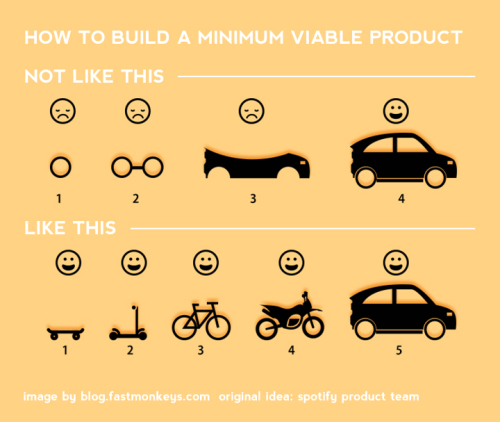
\includegraphics[width=0.6\linewidth]{img/spotify-howtobuildmvp} \caption{From ["Your ultimate guide to Minimum Viable Product (+great examples)"](https://blog.fastmonkeys.com/2014/06/18/minimum-viable-product-your-ultimate-guide-to-mvp-great-examples/)}\label{fig:spotify-howtobuildmvp}
\end{figure}

Build that skateboard before you build the car or some fancy car part. A limited-but-functioning thing is very useful. It also keeps the spirits high.

This is related to the valuable \href{http://c2.com/cgi/wiki?TelescopeRule}{Telescope Rule}:

\begin{quote}
It is faster to make a four-inch mirror then a six-inch mirror than to make a six-inch mirror.
\end{quote}

\hypertarget{turn-the-working-interactive-code-into-a-function}{%
\section{Turn the working interactive code into a function}\label{turn-the-working-interactive-code-into-a-function}}

Add NO new functionality! Just write your very first R function.

\begin{Shaded}
\begin{Highlighting}[]
\NormalTok{max_minus_min <-}\StringTok{ }\ControlFlowTok{function}\NormalTok{(x) }\KeywordTok{max}\NormalTok{(x) }\OperatorTok{-}\StringTok{ }\KeywordTok{min}\NormalTok{(x)}
\KeywordTok{max_minus_min}\NormalTok{(gapminder}\OperatorTok{$}\NormalTok{lifeExp)}
\CommentTok{#> [1] 59}
\end{Highlighting}
\end{Shaded}

Check that you're getting the same answer as you did with your interactive code. Test it eyeball-o-metrically at this point.

\hypertarget{test-your-function}{%
\section{Test your function}\label{test-your-function}}

\hypertarget{test-on-new-inputs}{%
\subsection{Test on new inputs}\label{test-on-new-inputs}}

Pick some new artificial inputs where you know (at least approximately) what your function should return.

\begin{Shaded}
\begin{Highlighting}[]
\KeywordTok{max_minus_min}\NormalTok{(}\DecValTok{1}\OperatorTok{:}\DecValTok{10}\NormalTok{)}
\CommentTok{#> [1] 9}
\KeywordTok{max_minus_min}\NormalTok{(}\KeywordTok{runif}\NormalTok{(}\DecValTok{1000}\NormalTok{))}
\CommentTok{#> [1] 0.997}
\end{Highlighting}
\end{Shaded}

I know that 10 minus 1 is 9. I know that random uniform {[}0, 1{]} variates will be between 0 and 1. Therefore max - min should be less than 1. If I take LOTS of them, max - min should be pretty close to 1.

It is intentional that I tested on integer input as well as floating point. Likewise, I like to use valid-but-random data for this sort of check.

\hypertarget{test-on-real-data-but-different-real-data}{%
\subsection{\texorpdfstring{Test on real data but \emph{different} real data}{Test on real data but different real data}}\label{test-on-real-data-but-different-real-data}}

Back to the real world now. Two other quantitative variables are lying around: \texttt{gdpPercap} and \texttt{pop}. Let's have a go.

\begin{Shaded}
\begin{Highlighting}[]
\KeywordTok{max_minus_min}\NormalTok{(gapminder}\OperatorTok{$}\NormalTok{gdpPercap)}
\CommentTok{#> [1] 113282}
\KeywordTok{max_minus_min}\NormalTok{(gapminder}\OperatorTok{$}\NormalTok{pop)}
\CommentTok{#> [1] 1318623085}
\end{Highlighting}
\end{Shaded}

Either check these results ``by hand'' or apply the ``does that even make sense?'' test.

\hypertarget{test-on-weird-stuff}{%
\subsection{Test on weird stuff}\label{test-on-weird-stuff}}

Now we try to break our function. Don't get truly diabolical (yet). Just make the kind of mistakes you can imagine making at 2 a.m. when, 3 years from now, you rediscover this useful function you wrote. Give your function inputs it's not expecting.

\begin{Shaded}
\begin{Highlighting}[]
\KeywordTok{max_minus_min}\NormalTok{(gapminder) }\CommentTok{## hey sometimes things "just work" on data.frames!}
\CommentTok{#> Error in FUN(X[[i]], ...): only defined on a data frame with all numeric variables}
\KeywordTok{max_minus_min}\NormalTok{(gapminder}\OperatorTok{$}\NormalTok{country) }\CommentTok{## factors are kind of like integer vectors, no?}
\CommentTok{#> Error in Summary.factor(structure(c(1L, 1L, 1L, 1L, 1L, 1L, 1L, 1L, 1L, : 'max' not meaningful for factors}
\KeywordTok{max_minus_min}\NormalTok{(}\StringTok{"eggplants are purple"}\NormalTok{) }\CommentTok{## i have no excuse for this one}
\CommentTok{#> Error in max(x) - min(x): non-numeric argument to binary operator}
\end{Highlighting}
\end{Shaded}

How happy are you with those error messages? You must imagine that some entire \textbf{script} has failed and that you were hoping to just \texttt{source()} it without re-reading it. If a colleague or future you encountered these errors, do you run screaming from the room? How hard is it to pinpoint the usage problem?

\hypertarget{i-will-scare-you-now}{%
\subsection{I will scare you now}\label{i-will-scare-you-now}}

Here are some great examples STAT 545 students devised during class where the function \textbf{should break but it does not.}

\begin{Shaded}
\begin{Highlighting}[]
\KeywordTok{max_minus_min}\NormalTok{(gapminder[}\KeywordTok{c}\NormalTok{(}\StringTok{'lifeExp'}\NormalTok{, }\StringTok{'gdpPercap'}\NormalTok{, }\StringTok{'pop'}\NormalTok{)])}
\CommentTok{#> [1] 1.32e+09}
\KeywordTok{max_minus_min}\NormalTok{(}\KeywordTok{c}\NormalTok{(}\OtherTok{TRUE}\NormalTok{, }\OtherTok{TRUE}\NormalTok{, }\OtherTok{FALSE}\NormalTok{, }\OtherTok{TRUE}\NormalTok{, }\OtherTok{TRUE}\NormalTok{))}
\CommentTok{#> [1] 1}
\end{Highlighting}
\end{Shaded}

In both cases, R's eagerness to make sense of our requests is unfortunately successful. In the first case, a data.frame containing just the quantitative variables is eventually coerced into numeric vector. We can compute max minus min, even though it makes absolutely no sense at all. In the second case, a logical vector is converted to zeroes and ones, which might merit an error or at least a warning.

\hypertarget{check-the-validity-of-arguments}{%
\section{Check the validity of arguments}\label{check-the-validity-of-arguments}}

For functions that will be used again -- which is not all of them! -- it is good to check the validity of arguments. This implements a rule from \href{http://www.faqs.org/docs/artu/ch01s06.html}{the Unix philosophy}:

\begin{quote}
Rule of Repair: When you must fail, fail noisily and as soon as possible.
\end{quote}

\hypertarget{stop-if-not}{%
\subsection{stop if not}\label{stop-if-not}}

\texttt{stopifnot()} is the entry level solution. I use it here to make sure the input \texttt{x} is a numeric vector.

\begin{Shaded}
\begin{Highlighting}[]
\NormalTok{mmm <-}\StringTok{ }\ControlFlowTok{function}\NormalTok{(x) \{}
  \KeywordTok{stopifnot}\NormalTok{(}\KeywordTok{is.numeric}\NormalTok{(x))}
  \KeywordTok{max}\NormalTok{(x) }\OperatorTok{-}\StringTok{ }\KeywordTok{min}\NormalTok{(x)}
\NormalTok{\}}
\KeywordTok{mmm}\NormalTok{(gapminder)}
\CommentTok{#> Error in mmm(gapminder): is.numeric(x) is not TRUE}
\KeywordTok{mmm}\NormalTok{(gapminder}\OperatorTok{$}\NormalTok{country)}
\CommentTok{#> Error in mmm(gapminder$country): is.numeric(x) is not TRUE}
\KeywordTok{mmm}\NormalTok{(}\StringTok{"eggplants are purple"}\NormalTok{)}
\CommentTok{#> Error in mmm("eggplants are purple"): is.numeric(x) is not TRUE}
\KeywordTok{mmm}\NormalTok{(gapminder[}\KeywordTok{c}\NormalTok{(}\StringTok{'lifeExp'}\NormalTok{, }\StringTok{'gdpPercap'}\NormalTok{, }\StringTok{'pop'}\NormalTok{)])}
\CommentTok{#> Error in mmm(gapminder[c("lifeExp", "gdpPercap", "pop")]): is.numeric(x) is not TRUE}
\KeywordTok{mmm}\NormalTok{(}\KeywordTok{c}\NormalTok{(}\OtherTok{TRUE}\NormalTok{, }\OtherTok{TRUE}\NormalTok{, }\OtherTok{FALSE}\NormalTok{, }\OtherTok{TRUE}\NormalTok{, }\OtherTok{TRUE}\NormalTok{))}
\CommentTok{#> Error in mmm(c(TRUE, TRUE, FALSE, TRUE, TRUE)): is.numeric(x) is not TRUE}
\end{Highlighting}
\end{Shaded}

And we see that it catches all of the self-inflicted damage we would like to avoid.

\hypertarget{if-then-stop}{%
\subsection{if then stop}\label{if-then-stop}}

\texttt{stopifnot()} doesn't provide a very good error message. The next approach is very widely used. Put your validity check inside an \texttt{if()} statement and call \texttt{stop()} yourself, with a custom error message, in the body.

\begin{Shaded}
\begin{Highlighting}[]
\NormalTok{mmm2 <-}\StringTok{ }\ControlFlowTok{function}\NormalTok{(x) \{}
  \ControlFlowTok{if}\NormalTok{(}\OperatorTok{!}\KeywordTok{is.numeric}\NormalTok{(x)) \{}
    \KeywordTok{stop}\NormalTok{(}\StringTok{'I am so sorry, but this function only works for numeric input!}\CharTok{\textbackslash{}n}\StringTok{'}\NormalTok{,}
         \StringTok{'You have provided an object of class: '}\NormalTok{, }\KeywordTok{class}\NormalTok{(x)[}\DecValTok{1}\NormalTok{])}
\NormalTok{  \}}
  \KeywordTok{max}\NormalTok{(x) }\OperatorTok{-}\StringTok{ }\KeywordTok{min}\NormalTok{(x)}
\NormalTok{\}}
\KeywordTok{mmm2}\NormalTok{(gapminder)}
\CommentTok{#> Error in mmm2(gapminder): I am so sorry, but this function only works for numeric input!}
\CommentTok{#> You have provided an object of class: tbl_df}
\end{Highlighting}
\end{Shaded}

In addition to a gratuitous apology, the error raised also contains two more pieces of helpful info:

\begin{itemize}
\tightlist
\item
  \emph{Which} function threw the error.
\item
  Hints on how to fix things: expected class of input vs.~actual class.
\end{itemize}

If it is easy to do so, I highly recommend this template: ``you gave me THIS, but I need THAT''.

\href{https://style.tidyverse.org}{The tidyverse style guide} has a very useful \href{https://style.tidyverse.org/error-messages.html}{chapter on how to construct error messages}.

\hypertarget{sidebar-non-programming-uses-for-assertions}{%
\subsection{Sidebar: non-programming uses for assertions}\label{sidebar-non-programming-uses-for-assertions}}

Another good use of this pattern is to leave checks behind in data analytical scripts. Consider our repetitive use of Gapminder in this course. Every time we load it, we inspect it, hoping to see the usual stuff. If we were loading from file (vs.~a stable data package), we might want to formalize our expectations about the number of rows and columns, the names and flavors of the variables, etc. This would alert us if the data suddenly changed, which can be a useful wake-up call in scripts that you re-run \emph{ad nauseam} on auto-pilot or non-interactively.

\hypertarget{wrap-up-and-whats-next}{%
\section{Wrap-up and what's next?}\label{wrap-up-and-whats-next}}

Here's the function we've written so far:

\begin{Shaded}
\begin{Highlighting}[]
\NormalTok{mmm2}
\CommentTok{#> function(x) \{}
\CommentTok{#>   if(!is.numeric(x)) \{}
\CommentTok{#>     stop('I am so sorry, but this function only works for numeric input!\textbackslash{}n',}
\CommentTok{#>          'You have provided an object of class: ', class(x)[1])}
\CommentTok{#>   \}}
\CommentTok{#>   max(x) - min(x)}
\CommentTok{#> \}}
\end{Highlighting}
\end{Shaded}

What we've accomplished:

\begin{itemize}
\tightlist
\item
  We've written our first function.
\item
  We are checking the validity of its input, argument \texttt{x}.
\item
  We've done a good amount of informal testing.
\end{itemize}

Where to next? In \protect\hyperlink{functions-part2}{part 2} we generalize this function to take differences in other quantiles and learn how to set default values for arguments.

\hypertarget{resources}{%
\section{Resources}\label{resources}}

\begin{itemize}
\tightlist
\item
  Packages for runtime assertions:

  \begin{itemize}
  \tightlist
  \item
    assertthat on \href{https://cloud.R-project.org/package=assertthat}{CRAN} and \href{https://github.com/hadley/assertthat}{GitHub} - \emph{the Hadleyverse option}
  \item
    ensurer on \href{https://cloud.R-project.org/package=ensurer}{CRAN} and \href{https://github.com/smbache/ensurer}{GitHub} - \emph{general purpose, pipe-friendly}
  \item
    assertr on \href{https://cloud.R-project.org/package=assertr}{CRAN} and \href{https://github.com/ropensci/assertr}{GitHub} - \emph{explicitly data pipeline oriented}
  \item
    assertive on \href{https://cloud.R-project.org/package=assertive}{CRAN} and \href{https://bitbucket.org/richierocks/assertive/src/master/}{Bitbucket} - \emph{rich set of built-in functions}
  \end{itemize}
\item
  Hadley Wickham's book, \href{http://adv-r.had.co.nz}{Advanced R} \citeyearpar{wickham2015a}:

  \begin{itemize}
  \tightlist
  \item
    Section on \href{http://adv-r.had.co.nz/Exceptions-Debugging.html\#defensive-programming}{defensive programming}
  \end{itemize}
\end{itemize}

\hypertarget{functions-part2}{%
\chapter{Write your own R functions, part 2}\label{functions-part2}}

\hypertarget{where-were-we-where-are-we-going}{%
\section{Where were we? Where are we going?}\label{where-were-we-where-are-we-going}}

In \protect\hyperlink{functions-part1}{part 1} we wrote our first R function to compute the difference between the max and min of a numeric vector. We checked the validity of the function's only argument and, informally, we verified that it worked pretty well.

In this part, we generalize this function, learn more technical details about R functions, and set default values for some arguments.

\hypertarget{load-the-gapminder-data}{%
\section{Load the Gapminder data}\label{load-the-gapminder-data}}

As usual, load \href{https://github.com/jennybc/gapminder}{gapminder}.

\begin{Shaded}
\begin{Highlighting}[]
\KeywordTok{library}\NormalTok{(gapminder)}
\end{Highlighting}
\end{Shaded}

\hypertarget{restore-our-max-minus-min-function}{%
\section{Restore our max minus min function}\label{restore-our-max-minus-min-function}}

Let's keep our previous function around as a baseline.

\begin{Shaded}
\begin{Highlighting}[]
\NormalTok{mmm <-}\StringTok{ }\ControlFlowTok{function}\NormalTok{(x) \{}
  \KeywordTok{stopifnot}\NormalTok{(}\KeywordTok{is.numeric}\NormalTok{(x))}
  \KeywordTok{max}\NormalTok{(x) }\OperatorTok{-}\StringTok{ }\KeywordTok{min}\NormalTok{(x)}
\NormalTok{\}}
\end{Highlighting}
\end{Shaded}

\hypertarget{generalize-our-function-to-other-quantiles}{%
\section{Generalize our function to other quantiles}\label{generalize-our-function-to-other-quantiles}}

The max and the min are special cases of a \textbf{quantile}. Here are other special cases you may have heard of:

\begin{itemize}
\tightlist
\item
  Median = 0.5 quantile
\item
  1st quartile = 0.25 quantile
\item
  3rd quartile = 0.75 quantile
\end{itemize}

If you're familiar with \href{https://en.wikipedia.org/wiki/Box_plot}{box plots}, the rectangle typically runs from the 1st quartile to the 3rd quartile, with a line at the median.

If \(q\) is the \(p\)-th quantile of a set of \(n\) observations, what does that mean? Approximately \(pn\) of the observations are less than \(q\) and \((1 - p)n\) are greater than \(q\). Yeah, you need to worry about rounding to an integer and less/greater than or equal to, but these details aren't critical here.

Let's generalize our function to take the difference between any two quantiles. We can still consider the max and min, if we like, but we're not limited to that.

\hypertarget{get-something-that-works-again}{%
\section{Get something that works, again}\label{get-something-that-works-again}}

The eventual inputs to our new function will be the data \texttt{x} and two probabilities.

First, play around with the \texttt{quantile()} function. Convince yourself you know how to use it, for example, by cross-checking your results with other built-in functions.

\begin{Shaded}
\begin{Highlighting}[]
\KeywordTok{quantile}\NormalTok{(gapminder}\OperatorTok{$}\NormalTok{lifeExp)}
\CommentTok{#>   0%  25%  50%  75% 100% }
\CommentTok{#> 23.6 48.2 60.7 70.8 82.6}
\KeywordTok{quantile}\NormalTok{(gapminder}\OperatorTok{$}\NormalTok{lifeExp, }\DataTypeTok{probs =} \FloatTok{0.5}\NormalTok{)}
\CommentTok{#>  50% }
\CommentTok{#> 60.7}
\KeywordTok{median}\NormalTok{(gapminder}\OperatorTok{$}\NormalTok{lifeExp)}
\CommentTok{#> [1] 60.7}
\KeywordTok{quantile}\NormalTok{(gapminder}\OperatorTok{$}\NormalTok{lifeExp, }\DataTypeTok{probs =} \KeywordTok{c}\NormalTok{(}\FloatTok{0.25}\NormalTok{, }\FloatTok{0.75}\NormalTok{))}
\CommentTok{#>  25%  75% }
\CommentTok{#> 48.2 70.8}
\KeywordTok{boxplot}\NormalTok{(gapminder}\OperatorTok{$}\NormalTok{lifeExp, }\DataTypeTok{plot =} \OtherTok{FALSE}\NormalTok{)}\OperatorTok{$}\NormalTok{stats}
\CommentTok{#>      [,1]}
\CommentTok{#> [1,] 23.6}
\CommentTok{#> [2,] 48.2}
\CommentTok{#> [3,] 60.7}
\CommentTok{#> [4,] 70.8}
\CommentTok{#> [5,] 82.6}
\end{Highlighting}
\end{Shaded}

Now write a code snippet that takes the difference between two quantiles.

\begin{Shaded}
\begin{Highlighting}[]
\NormalTok{the_probs <-}\StringTok{ }\KeywordTok{c}\NormalTok{(}\FloatTok{0.25}\NormalTok{, }\FloatTok{0.75}\NormalTok{)}
\NormalTok{the_quantiles <-}\StringTok{ }\KeywordTok{quantile}\NormalTok{(gapminder}\OperatorTok{$}\NormalTok{lifeExp, }\DataTypeTok{probs =}\NormalTok{ the_probs)}
\KeywordTok{max}\NormalTok{(the_quantiles) }\OperatorTok{-}\StringTok{ }\KeywordTok{min}\NormalTok{(the_quantiles)}
\CommentTok{#> [1] 22.6}
\end{Highlighting}
\end{Shaded}

\hypertarget{turn-the-working-interactive-code-into-a-function-again}{%
\section{Turn the working interactive code into a function, again}\label{turn-the-working-interactive-code-into-a-function-again}}

I'll use \texttt{qdiff} as the base of our function's name. I copy the overall structure from our previous ``max minus min'' work but replace the guts of the function with the more general code we just developed.

\begin{Shaded}
\begin{Highlighting}[]
\NormalTok{qdiff1 <-}\StringTok{ }\ControlFlowTok{function}\NormalTok{(x, probs) \{}
  \KeywordTok{stopifnot}\NormalTok{(}\KeywordTok{is.numeric}\NormalTok{(x))}
\NormalTok{  the_quantiles <-}\StringTok{ }\KeywordTok{quantile}\NormalTok{(}\DataTypeTok{x =}\NormalTok{ x, }\DataTypeTok{probs =}\NormalTok{ probs)}
  \KeywordTok{max}\NormalTok{(the_quantiles) }\OperatorTok{-}\StringTok{ }\KeywordTok{min}\NormalTok{(the_quantiles)}
\NormalTok{\}}
\KeywordTok{qdiff1}\NormalTok{(gapminder}\OperatorTok{$}\NormalTok{lifeExp, }\DataTypeTok{probs =} \KeywordTok{c}\NormalTok{(}\FloatTok{0.25}\NormalTok{, }\FloatTok{0.75}\NormalTok{))}
\CommentTok{#> [1] 22.6}
\KeywordTok{IQR}\NormalTok{(gapminder}\OperatorTok{$}\NormalTok{lifeExp) }\CommentTok{# hey, we've reinvented IQR}
\CommentTok{#> [1] 22.6}
\KeywordTok{qdiff1}\NormalTok{(gapminder}\OperatorTok{$}\NormalTok{lifeExp, }\DataTypeTok{probs =} \KeywordTok{c}\NormalTok{(}\DecValTok{0}\NormalTok{, }\DecValTok{1}\NormalTok{))}
\CommentTok{#> [1] 59}
\KeywordTok{mmm}\NormalTok{(gapminder}\OperatorTok{$}\NormalTok{lifeExp)}
\CommentTok{#> [1] 59}
\end{Highlighting}
\end{Shaded}

Again we do some informal tests against familiar results and external implementations.

\hypertarget{argument-names-freedom-and-conventions}{%
\section{Argument names: freedom and conventions}\label{argument-names-freedom-and-conventions}}

I want you to understand the importance of argument names.

I can name my arguments almost anything I like. Proof:

\begin{Shaded}
\begin{Highlighting}[]
\NormalTok{qdiff2 <-}\StringTok{ }\ControlFlowTok{function}\NormalTok{(zeus, hera) \{}
  \KeywordTok{stopifnot}\NormalTok{(}\KeywordTok{is.numeric}\NormalTok{(zeus))}
\NormalTok{  the_quantiles <-}\StringTok{ }\KeywordTok{quantile}\NormalTok{(}\DataTypeTok{x =}\NormalTok{ zeus, }\DataTypeTok{probs =}\NormalTok{ hera)}
  \KeywordTok{max}\NormalTok{(the_quantiles) }\OperatorTok{-}\StringTok{ }\KeywordTok{min}\NormalTok{(the_quantiles)}
\NormalTok{\}}
\KeywordTok{qdiff2}\NormalTok{(}\DataTypeTok{zeus =}\NormalTok{ gapminder}\OperatorTok{$}\NormalTok{lifeExp, }\DataTypeTok{hera =} \DecValTok{0}\OperatorTok{:}\DecValTok{1}\NormalTok{)}
\CommentTok{#> [1] 59}
\end{Highlighting}
\end{Shaded}

While I can name my arguments after Greek gods, it's usually a bad idea. Take all opportunities to make things more self-explanatory via meaningful names.

If you are going to pass the arguments of your function as arguments of a built-in function, consider copying the argument names. Unless you have a good reason to do your own thing (some argument names are bad!), be consistent with the existing function. Again, the reason is to reduce your cognitive load. This is what I've been doing all along and now you know why:

\begin{Shaded}
\begin{Highlighting}[]
\NormalTok{qdiff1}
\CommentTok{#> function(x, probs) \{}
\CommentTok{#>   stopifnot(is.numeric(x))}
\CommentTok{#>   the_quantiles <- quantile(x = x, probs = probs)}
\CommentTok{#>   max(the_quantiles) - min(the_quantiles)}
\CommentTok{#> \}}
\CommentTok{#> <bytecode: 0x7f931961d0a0>}
\end{Highlighting}
\end{Shaded}

We took this detour so you could see there is no \emph{structural} relationship between my arguments (\texttt{x} and \texttt{probs}) and those of \texttt{quantile()} (also \texttt{x} and \texttt{probs}). The similarity or equivalence of the names \textbf{accomplishes nothing} as far as R is concerned; it is solely for the benefit of humans reading, writing, and using the code. Which is very important!

\hypertarget{what-a-function-returns}{%
\section{What a function returns}\label{what-a-function-returns}}

By this point, I expect someone will have asked about the last line in my function's body. Look above for a reminder of the function's definition.

By default, a function returns the result of the last line of the body. I am just letting that happen with the line \texttt{max(the\_quantiles)\ -\ min(the\_quantiles)}. However, there is an explicit function for this: \texttt{return()}. I could just as easily make this the last line of my function's body:

\begin{Shaded}
\begin{Highlighting}[]
\KeywordTok{return}\NormalTok{(}\KeywordTok{max}\NormalTok{(the_quantiles) }\OperatorTok{-}\StringTok{ }\KeywordTok{min}\NormalTok{(the_quantiles))}
\end{Highlighting}
\end{Shaded}

You absolutely must use \texttt{return()} if you want to return early based on some condition, i.e.~before execution gets to the last line of the body. Otherwise, you can decide your own conventions about when you use \texttt{return()} and when you don't.

\hypertarget{default-values-freedom-to-not-specify-the-arguments}{%
\section{Default values: freedom to NOT specify the arguments}\label{default-values-freedom-to-not-specify-the-arguments}}

What happens if we call our function but neglect to specify the probabilities?

\begin{Shaded}
\begin{Highlighting}[]
\KeywordTok{qdiff1}\NormalTok{(gapminder}\OperatorTok{$}\NormalTok{lifeExp)}
\CommentTok{#> Error in quantile(x = x, probs = probs): argument "probs" is missing, with no default}
\end{Highlighting}
\end{Shaded}

Oops! At the moment, this causes a fatal error. It can be nice to provide some reasonable default values for certain arguments. In our case, it would be crazy to specify a default value for the primary input \texttt{x}, but very kind to specify a default for \texttt{probs}.

We started by focusing on the max and the min, so I think those make reasonable defaults. Here's how to specify that in a function definition.

\begin{Shaded}
\begin{Highlighting}[]
\NormalTok{qdiff3 <-}\StringTok{ }\ControlFlowTok{function}\NormalTok{(x, }\DataTypeTok{probs =} \KeywordTok{c}\NormalTok{(}\DecValTok{0}\NormalTok{, }\DecValTok{1}\NormalTok{)) \{}
  \KeywordTok{stopifnot}\NormalTok{(}\KeywordTok{is.numeric}\NormalTok{(x))}
\NormalTok{  the_quantiles <-}\StringTok{ }\KeywordTok{quantile}\NormalTok{(x, probs)}
  \KeywordTok{max}\NormalTok{(the_quantiles) }\OperatorTok{-}\StringTok{ }\KeywordTok{min}\NormalTok{(the_quantiles)}
\NormalTok{\}}
\end{Highlighting}
\end{Shaded}

Again we check how the function works, in old examples and new, specifying the \texttt{probs} argument and not.

\begin{Shaded}
\begin{Highlighting}[]
\KeywordTok{qdiff3}\NormalTok{(gapminder}\OperatorTok{$}\NormalTok{lifeExp)}
\CommentTok{#> [1] 59}
\KeywordTok{mmm}\NormalTok{(gapminder}\OperatorTok{$}\NormalTok{lifeExp)}
\CommentTok{#> [1] 59}
\KeywordTok{qdiff3}\NormalTok{(gapminder}\OperatorTok{$}\NormalTok{lifeExp, }\KeywordTok{c}\NormalTok{(}\FloatTok{0.1}\NormalTok{, }\FloatTok{0.9}\NormalTok{))}
\CommentTok{#> [1] 33.6}
\end{Highlighting}
\end{Shaded}

\hypertarget{check-the-validity-of-arguments-again}{%
\section{Check the validity of arguments, again}\label{check-the-validity-of-arguments-again}}

\textbf{Exercise:} upgrade our argument validity checks in light of the new argument \texttt{probs}.

\begin{Shaded}
\begin{Highlighting}[]
\CommentTok{## problems identified during class}
\CommentTok{## we're not checking that probs is numeric}
\CommentTok{## we're not checking that probs is length 2}
\CommentTok{## we're not checking that probs are in [0,1]}
\end{Highlighting}
\end{Shaded}

\hypertarget{wrap-up-and-whats-next}{%
\section{Wrap-up and what's next?}\label{wrap-up-and-whats-next}}

Here's the function we've written so far:

\begin{Shaded}
\begin{Highlighting}[]
\NormalTok{qdiff3}
\CommentTok{#> function(x, probs = c(0, 1)) \{}
\CommentTok{#>   stopifnot(is.numeric(x))}
\CommentTok{#>   the_quantiles <- quantile(x, probs)}
\CommentTok{#>   max(the_quantiles) - min(the_quantiles)}
\CommentTok{#> \}}
\CommentTok{#> <bytecode: 0x7f931a5e57b0>}
\end{Highlighting}
\end{Shaded}

What we've accomplished:

\begin{itemize}
\tightlist
\item
  We've generalized our first function to take a difference between arbitrary quantiles.
\item
  We've specified default values for the probabilities that set the quantiles.
\end{itemize}

Where to next? In \protect\hyperlink{functions-part3}{part 3} we tackle \texttt{NA}s, the special \texttt{...} argument, and formal unit testing.

\hypertarget{resources}{%
\section{Resources}\label{resources}}

\begin{itemize}
\tightlist
\item
  Hadley Wickham's book, \href{http://adv-r.had.co.nz}{Advanced R} \citeyearpar{wickham2015a}:

  \begin{itemize}
  \tightlist
  \item
    Section on \href{http://adv-r.had.co.nz/Functions.html\#function-arguments}{function arguments}
  \item
    Section on \href{http://adv-r.had.co.nz/Functions.html\#return-values}{return values}
  \end{itemize}
\end{itemize}

  \bibliography{book.bib,packages.bib}

\end{document}
